% LaTeX Template
% This template is made for project reports
% 	You may adjust it to your own needs/purposesF

% Copyright: http://www.howtotex.com/
% Date: March 2011

%\RequirePackage[log]{snapshot}

%%% Preamble
\PassOptionsToPackage{table}{xcolor}
\documentclass[12pt, a4paper, oneside, slovene]{article}
%\documentclass[paper=a4, fontsize=12pt]{scrartcl}	% Article class of KOMA-script with 11pt font and a4 format
\usepackage[a4paper, left=2.5cm, right=2.5cm, top=2.5cm, bottom=2.5cm, bindingoffset=0.5cm]{geometry}

%\setlength{\oddsidemargin}{5mm}
%\setlength{\evensidemargin}{5mm}

\usepackage[T1]{fontenc}
\usepackage{fourier}

\usepackage[utf8x]{inputenc}
\usepackage[slovene]{babel}															% English language/hyphenation
\usepackage[protrusion=true,expansion=true]{microtype}				% Better typography
\usepackage{amsmath,amsfonts,amsthm}										% Math packages
%\usepackage[pdftex]{graphicx}
\usepackage{graphicx}
\usepackage{grffile}
%\graphicspath{{./svg}}
%\graphicspath{{./poglavja/}}

% Enable pdflatex
%\usepackage{pdfpages}

%\usepackage{import}

\usepackage{url}
\usepackage[unicode]{hyperref}

\usepackage{lscape}

%%% Custom sectioning (sectsty package)
\usepackage{sectsty}
% Custom sectioning (see below)
%\allsectionsfont{\normalfont\scshape}	% Change font of al section
                                % commands
\allsectionsfont{\normalfont}	% Change font of al section commands

\usepackage[shortlabels]{enumitem}
\setlist{nosep} %%Zmanjša razdaljo med okolji za seznami in besedilom!cg

\usepackage{setspace}

%%% Custom headers/footers (fancyhdr package)
%%Fancy boxes

\usepackage{fancyhdr}

\setlength{\headheight}{13.6pt}
%\setlength{\footheight}{13.6pt}

\fancypagestyle{mainstyle}{
  \fancyhf{}
  \lfoot[\thepage]{}
  \rfoot[]{\thepage}

  \renewcommand{\headrulewidth}{0pt}			% Remove header underlines
  \renewcommand{\footrulewidth}{0pt}				% Remove footer underlines
}

\fancypagestyle{beginstyle}{
  \fancyhf{}
  \rfoot[\thepage]{\thepage}
  \renewcommand{\headrulewidth}{0pt}			% Remove header underlines
  \renewcommand{\footrulewidth}{0pt}				% Remove footer underlines
}




\usepackage[pdftex,dvipsnames,table,x11names,rgb,html]{xcolor}

\usepackage{wrapfig}
\usepackage{subcaption}
%%%Nastavitve barv
\definecolor{airforceblue}{rgb}{0.36, 0.54, 0.66}

%% \usepackage{solarized-light} to so nastavitve, ki določajo barvno
%% shemo za solarized prenesene so zaradi overleaf.com

%Nastavitve barv za Solarized

\definecolor{sbase03}{HTML}{002B36}
\definecolor{sbase02}{HTML}{073642}
\definecolor{sbase01}{HTML}{586E75}
\definecolor{sbase00}{HTML}{657B83}
\definecolor{sbase0}{HTML}{839496}
\definecolor{sbase1}{HTML}{93A1A1}
\definecolor{sbase2}{HTML}{EEE8D5}
\definecolor{sbase3}{HTML}{FDF6E3}
\definecolor{syellow}{HTML}{B58900}
\definecolor{sorange}{HTML}{CB4B16}
\definecolor{sred}{HTML}{DC322F}
\definecolor{smagenta}{HTML}{D33682}
\definecolor{sviolet}{HTML}{6C71C4}
\definecolor{sblue}{HTML}{268BD2}
\definecolor{scyan}{HTML}{2AA198}
\definecolor{sgreen}{HTML}{859900}

%Nastavitve za prikaz barvanja kode!
\usepackage{listings}
\lstset{
    % How/what to match
    sensitive=true,
    % Border (above and below)
    frame=none,
    % Extra margin on line (align with paragraph)
    xleftmargin=\parindent,
    % Put extra space under caption
    belowcaptionskip=1\baselineskip,
    % Colors
    rulecolor=\color{sbase1},
    backgroundcolor=\color{sbase3},
    basicstyle=\color{sbase00}\ttfamily\footnotesize,
    keywordstyle=\color{scyan},
    commentstyle=\color{sbase1},
    stringstyle=\color{sblue},
    numberstyle=\color{sbase1},
    identifierstyle=\color{sbase00},
    % Break long lines into multiple lines?
    breaklines=true,
    % Show a character for spaces?
    showstringspaces=false,
    tabsize=2,
    numbers=left,                    % where to put the line-numbers; possible values are (none, left, right)
    numbersep=5pt,                   % how far the line-numbers are from the code
    numberstyle=\footnotesize,        %\color{mygray}, % the style
                                %that
   % inputencoding=utf8,
    extendedchars=true,
    literate=
    {š}{{\v{s}}}1
    {č}{{\v{c}}}1
    {ž}{{\v{z}}}1
}

\usepackage{fancyvrb}

%%Barvne škatle
\usepackage{tcolorbox}
%ustvarjanje lastnoe barvne škatle!
\newtcolorbox[auto counter]{examplebox}[2][]{%
colframe=sbase02!100,
colback=sbase3!100,
coltitle=sbase1!100!black,
colupper=sbase01!100!black,
collower=sbase01!100!black,
fonttitle=\bfseries,
title=Primer ~\thetcbcounter: #2,#1
}


%ustvarjanje lastnoe barvne škatle za osebno posameznega portala!
\newtcolorbox[auto counter]{osebnabox}[2][]{%
colframe=sbase02!100,
colback=sbase3!100,
coltitle=sbase1!100!black,
colupper=sbase01!100!black,
collower=sbase01!100!black,
fonttitle=\bfseries,
title= #2,#1
}


\usepackage{xargs}  %Uporabei več kot en argument v novem ukazu
%Paket za dodajanje todo oblačkov!
\usepackage[colorinlistoftodos,prependcaption,textsize=tiny]{todonotes}
%\newcommandx{\unsure}[2][1=]{\todo[linecolor=red,backgroundcolor=red!25,bordercolor=red,#1]{#2}}
\newcommandx{\TODO}[2][1=]{\todo[linecolor=blue,backgroundcolor=blue!25,bordercolor=blue,#1]{#2}}
\newcommand{\inlcomment}{\info[inline]{1=}}
%%% Equation and float numbering
%\numberwithin{equation}{section}		% Equationnumbering: section.eq#
%\numberwithin{figure}{section}			% Figurenumbering: section.fig#
%\numberwithin{table}{section}		        % Tablenumbering: section.tab#

%Nastavitve odstavkov
\setlength{\parindent}{0cm}
\setlength{\parskip}{10px}

%Prostor med vrsticami
%\singlespacing
\onehalfspacing

%%Diferent enumeration
%\usepackage{enumerate}

%%Pandoc workaroun \tightlisr
\providecommand{\tightlist}{%
  \setlength{\itemsep}{0pt}\setlength{\parskip}{0pt}}


%\usepackage[table]{xcolor}
%%Ne preverja če napis gre v eno vrstico in ga zato ne premakne na sredino.
\usepackage[singlelinecheck=false]{caption}


%%% Maketitle metadata
\newcommand{\horrule}[1]{\rule{\linewidth}{#1}} 	% Horizontal rule
%%% Begin document

%%%


%Spremenljivke

%Ustanova
\newcommand{\univerza}{Univerza v Mariboru}
\newcommand{\UNIVERZA}{UNIVERZA V MARIBORU}
\newcommand{\fakulteta}{Fakulteta za naravoslovje in matematiko}
\newcommand{\FAKULTETA}{FAKULTETA ZA NARAVOSLOVJE IN MATEMATIKO}
\newcommand{\naslovfak}{Koroška cesta 160, 2000 Maribor}
\newcommand{\oddelek}{Oddelek za matematiko in računalništvo}

%Naslov
\newcommand{\naslov}{DIPLOMSKO DELO}
\newcommand{\podnaslov}{Spletni
  portali za učenje programiranja: klasifikacija in možnosti uporabe v
  izobraževanju}

% Mentor/profesor
\newcommand{\mentor}{doc. dr. Igor Pesek}

% Študent
\newcommand{\kandidat}{Gregor Nemec}
\newcommand{\program}{Fizika in računalništvo}
\newcommand{\letnik}{4.letnik}
\newcommand{\smer}{Fizika in računalništvo}
\newcommand{\email}{gregorneme@gmail.com}

% Naslov, datum

\newcommand{\datum}{Maribor, 2016}

%Začetek dokumenta

\begin{document}

\thispagestyle{empty}
%%% Document title variables

%%%%%%%%%%%%%%%%%%%%%%%%%%%%%%%%%%%%%%%%%%%%%%%%%%%%%%%%%%%%%% 
% NASLOVNICA
%%%%%%%%%%%%%%%%%%%%%%%%%%%%%%%%%%%%%%%%%%%%%%%%%%%%%%%%%%%%%% 
\pagestyle{empty}
% ---------======== Naslovnica =======----------
\begin{center}
  \large
  \UNIVERZA

  \FAKULTETA

  \oddelek

\end{center}

\vspace{4cm}


\begin{center}
  \vspace{1cm}
  {\Huge \bfseries \naslov}\\
  \vspace{2cm}
  {\Large \kandidat}
\end{center}
\vspace*{\fill}
\vspace*{\fill}

% \begin{flushleft}
%   % \vspace{1cm}
%   \Large \mentor
% \end{flushleft}

\begin{center}


  \vspace{2cm}


  {\large \datum}
\end{center}


% ---------======== Naslovnica =======----------

%%% Local Variables:
%%% mode: latex
%%% TeX-master: "diploma"
%%% End:

\newpage
\thispagestyle{empty}
 % ---------======== Podnaslovnica =======----------

  \begin{center}
    \large
    \univerza

    \fakulteta

    \oddelek
  \end{center}

  \vspace{3cm}


  \begin{center}
    {\Large Diplomsko delo}

    \vspace{1cm}
    {\Huge \bfseries \podnaslov
      \vspace{1cm} DIPLOMSKEGA DELA
      %\vspace{1cm} (*ustrezno spremeniti*)}


    \vspace{5cm}

    \begin{flushleft}
      Mentor: \hspace{\stretch{2.8}} Kandidat:


      \mentor  \hspace{\stretch{2.3}} \kandidat
    \end{flushleft}


    \vspace{3cm}
    {\large \datum}
  \end{center}

 % ---------======== podnaslovnica =======----------


%%% Local Variables:
%%% mode: latex
%%% TeX-master: "diploma"
%%% End:

\newpage
\thispagestyle{empty}
% --------------------------------------------
  % ---------======== Zahvala =======-----------
  % --------------------------------------------

  \begin{center}
    \Large
    ZAHVALA
  \end{center}

  \vspace{1cm}

  % \begin{flushright}
  \textit{Citat\\
    verz (mo\v zna opcija)(*ustrezno spremeniti*)}
  % \end{flushright}

  \vspace{2cm}

  \begin{sloppypar}
    \textit{Zahvala...(*ustrezno spremeniti*)}
  \end{sloppypar}

  \begin{sloppypar}
    \textit{Posebna hvala  \v se...(*ustrezno spremeniti*)}
  \end{sloppypar}



  \vspace{1cm}
  \begin{sloppypar}

    \textit{Vsem iskreno hvala.(*ustrezno spremeniti*)}
  \end{sloppypar}

  \vfill


%%% Local Variables:
%%% mode: latex
%%% TeX-master: "diploma"
%%% End:
\newpage
\pagestyle{beginstyle}
\pagenumbering{Roman}
\setcounter{page}{4}
% --------------------------------------------
  % ---------======== Izjava =======------------
  % --------------------------------------------
  \newpage

  \begin{center}
    \large
    UNIVERZA V MARIBORU

    FAKULTETA ZA NARAVOSLOVJE IN MATEMATIKO

  \end{center}

  \vspace{3cm}

  \begin{center}
    \large
    IZJAVA
  \end{center}

  \vspace{2cm}
  Podpisani/a Ime Priimek, rojen/a xx. meseca 19xx(*ustrezno spremeniti*), \v student/ka Fakultete za
  naravoslovje in matematiko Univerze v Mariboru,
  \v studijskega programa matematika/ vpisati drug ustrezen program, izjavljam,
  da je diplomsko delo z naslovom


  \begin{center}
    NASLOV DIPLOMSKEGA DELA(*ustrezno spremeniti*)
  \end{center}


  pri mentorju prof. dr. Ime Priimek(*ustrezno spremeniti*)
  avtorsko delo. V diplomskem delu so uporabljeni viri in
pppp  literatura korektno navedeni; teksti niso uporabljeni
  brez navedbe avtorjev.
  \vspace{4cm}

  Maribor, xx. mesec 2015
  (*podpi\v se kandidat*)

  \vspace{1cm}
  \begin{flushright}
    Ime Priimek\\
  \end{flushright}



%%% Local Variables:
%%% mode: latex
%%% TeX-master: "diploma"
%%% End:
\newpage
\begin{center}
\section*{\podnaslov}
\textbf{Program diplomskega dela}
\end{center}

S trendom popularizacije programiranja, so se v zadnjem času pojavili spletni
portali, kot je, ki omogočajo spletno učenje programiranja in kodiranja. V
diplomskega dela določite kriterije in z njimi ovrednotite posamezne portale.
Raziščite možne načine uporabe spletnih portalov in podajte ideje kako bi jih
lahko umestili v pouk računalništva v OŠ in SŠ.

\textbf{Viri:}
\begin{itemize}
\item S.C. Ng, S.O Choy, R. Kwan, S.F. Chan, ''A Web-Based Environment to
  Improve Teaching and Learning of Computer Programming in Distance Education'',
  \emph{ICWL'05 Proceedings of the 4th international conference on Advances in
    Web-Based Learning}, 2005.
\item L. Ma, J. D. Ferguson, M. Roper, I.Ross, M. Wood, ''A web-based learning
  model for improving programming students' mental models'', v \emph{Proceedings
    of the 9th annual conference of the subject centre for information and
    computer sciences}, HE Academy, 2008 pp. 88-94.
\item  O. Hazzan, T. Lapidot, N. Ragonis, \emph{Guide to Teaching Computer
    Science}, Springer, 2011.
\end{itemize}

\vspace{2cm}
\begin{flushright}
\mentor
\end{flushright}


%%% Local Variables:
%%% mode: latex
%%% TeX-master: "diploma"
%%% End:

\newpage
\textbf{Nemec, G.: \podnaslov. Diplomsko delo, \univerza, \fakulteta,
Oddelek za matematiko in računalništvo, 2016.}

\section*{Povzetek}
\label{sec:povzetek}

V zadnjem času so se pojavili številni spletni portali, ki ponujajo učenje
programiranja. V diplomskem delu nas zanima, kateri so ti spletni portali in
kako jih lahko umestimo v pouk v osnovnih in srednjih šolah. V ta namen smo
pregledali spletne portale, ki so nastali v akademskem okolju ter določili
kriterije, ki so bili glavno vodilo pri klasifikaciji in vrednotenju spletnih
portalov. Novonastalih portalov je precej, zato smo izbiro omejili s kriteriji,
kot je brezplačen dostop do gradiv in zmožnost napredno kombiniranih vsebin.
Pregled portalov je pokazal, da vsak izmed njih prinaša številne zmožnosti pri
uporabi, izpostavili smo tudi nekatere slabosti. S konkretnima primeroma smo
pokazali, kako bi lahko uporabili spletni portal pri pouku.


\textbf{Ključne besede:} Učenje programiranja, spletni portali, programski
jeziki. 

%%% Local Variables:
%%% mode: latex
%%% TeX-master: "diploma"
%%% End:

\newpage
\textbf{Nemec, G.: angleški naslov. Graduation Thesis, University of
  Maribor, Faculty of Natural Sciences and Mathematics, Department of
  Computer Science, 2016.}

\section*{Abstract}
\label{sec:abstract}


Key words: 


%%% Local Variables:
%%% mode: latex
%%% TeX-master: "diploma"
%%% End:

\newpage
\let\tempmargin\oddsidemargin
\let\oddsidemargin\evensidemargin
\let\evensidemargin\tempmargin
\reversemarginpar
\newgeometry{a4paper, left=2.5cm, right=2.5cm, top=2.5cm, bottom=2.5cm,
  bindingoffset=0.5cm, twoside}
\pagestyle{mainstyle}
\pagenumbering{arabic}
\setcounter{page}{1}
\tableofcontents
\newpage
\listoftables
\newpage
\listoffigures
\newpage
%%Seznam kratic, ki se uporablja čez diplomsko delo.

\section*{Pregled uporabljenih simbolov in označb}
\label{sec:pregled_uporabljenih_simbolov_in_označb}

\begin{enumerate}[leftmargin=*]
\item \textbf{IKT} - informacijsko komunikacijska tehnologija;
\item \textbf{SPUP} - spletni portal za učenje programiranja;
\item \textbf{SPZP} - spletna aplikacija za programiranje;
\item \textbf{AVP} - aplikacijski programski vmesnik
  (\emph{ang. application programming interface \textbf{API}});
\end{enumerate}




%%% Local Variables:
%%% mode: latex
%%% TeX-master: "diploma"
%%% End:

\newpage
\section{Uvod}
\label{sec:Uvod}

% Originalna dispozicija: S trendom popularizacije programiranja, so
% se v zadnjem času pojavili spletni portali, kot je Codeacademy, ki
% omogočajo spletno učenje programiranja in kodiranja. V diplomskega
% dela določite kriterije in z njimi ovrednotite posamezne portale.
% Raziščite možne načine uporabe spletnih portalov in podajte ideje
% kako bi jih lahko umestili v pouk računalništva v OŠ in SŠ.

V svetovnem merilu se pojavlja trend po popularizaciji programiranja
in kodiranja. V zadnjem obdobju so se na spletu pojavili številni
portali, kot je na primer
\emph{\href{https://www.codecademy.com/}{Codeacademy}}
\cite{web:codeacademy}, ki ponujajo učenje programiranja. Zanima nas
kateri so ti portali, katere vsebine ponujajo, na kakšen način so
vsebine predstavljene in ali so uporabni za uporabo pri pouku ter na
kakšen način bi jih lahko uporabili.

Najprej bomo raziskali kako je definirana računalniška pismenost in
uporaba računalnika pri pouku. Ogledali si bomo kje se uči
programiranja na osnovni (\textbf{OŠ})in srednji šoli
(\textbf{SŠ}). Pri katerih izbirnih vsebinah, predmetih in kakšna je
vsebina, ki jo predvideva učni načrt. Podrobneje bomo preučili vse
tiste pojme, ki se pojavljajo v računalniški znanosti in
programiranju, ki nam bodo pomagali bolje razumeti spletne portale in
vsebino, ki jo predstavljajo.  Preučili bodo tudi sodobne pristope in
strategije, ki se uporabljajo pri učenju programiranja, saj bomo tako
lažje ocenili ali jih spletni portali tudi znajo upoštevati.

Zanimali nas bodo \textbf{novinci} in njihove težave pri začetnih
korakih učenja programiranja. Ko govorimo o novincih imamo v mislih
vse tiste učence, dijake in študente, ki se šele srečujejo s
programiranjem, ne glede na spol. Prav tako nas bodo zanimali
\textbf{mentorji} s katerim imamo v mislih učitelje in profesorje.

V ta namen bomo pregledali nastanek spletnih portalov za namen učenja
programiranja, ki so se pojavila v akademskem okolju na posameznih
univerzah. Zanimal nas bo razlog za nastanek takšnih spletni portalov
na univerzah, zato bomo pregledali literaturo in poskusimo ugotoviti,
zakaj in kako se na višje šolskem področju uporabljajo spletne
tehnologije za poučevanje programiranja in kako so skušale premostiti
nekatere težave, ki jih imajo novinci pri učenju programiranja.

Izluščili bomo predlagane rešitve za uporabo spletnih tehnologij pri
učenje programiranja. Na podlagi pregledanega bomo lahko določili
kriterije s katerimi bomo lahko klasificirali spletne portale in jih
tudi ovrednotili ter uspešno umestili v pouk.

%Vpelji novinec, učenec, dijak isto za mentorja. 

%%% Local Variables:
%%% mode: latex
%%% TeX-master: "../diploma"
%%% End:


\newpage
\section{Uporaba računalnika v izobraževanju}
\label{sec:uporaba-raunalnika-v}

Model uporabe računalnika v izobraževanju je Gerlič \cite{gerlic_2000}
razdelil na tri področja. V \textbf{primarno področje} lahko uvrstimo
učenje računalništva in programiranja, saj sem prištevamo aktivnosti s
katerimi želimo uporabnike seznaniti z delovanjem in uporabo
računalnika oz. sodobno informacijsko komunikacijsko tehnologijo
(\textbf{IKT}). Računalnik je tista učna vsebina, ki jo
obravnavamo. \textbf{Sekundarno področje} predstavlja vse tiste
aktivnosti, katere so vezane neposredno na izobraževalni proces
katerega koli predmetnega področja. Računalnik in IKT nastopata kot
učno sredstvo ali pripomoček v oblikah tradicionalnih računalniško
podprtih učnih sistemov ali inteligentnih ekspertnih sistemov. V
\textbf{terciarno področje}, spadajo vse aktivnosti, ki spremljajo
izobraževanje. Sem se štejejo aktivnosti izobraževanja, vodenja in
upravljanja izobraževalnega sistema.

V tem diplomskem delu nas bo zanimalo le \textbf{primarno področje}
uporabe računalnika v izobraževanju, ki je razdeljeno v dveh pomembnih
področjih \cite{gerlic_2000}:

\begin{itemize}
\tightlist
\item kot element \textbf{splošne izobrazbe},
\item kot element \textbf{ožje strokovne} - poklicne izobrazbe
  oz. usposabljanja.
\end{itemize}

\subsection{Splošnoizobraževalno področje}
\label{sec:spološnoiz_področje}

V današnjem času se računalnik kot element splošne izobrazbe kaže kot
velika potreba oz. se zdi znanje njegove uporabe samoumevno. Že pri
najmlajših otrocih računalnik vzbuja zanimanje in interes.  Računalnik
je postal intelektualno orodje in pripomoček v vsaki sferi človekove
dejavnosti in je prodrl že dolgo nazaj tudi v šolo. Tako imenovana
\textbf{računalniška pismenost} postaja nuja in zajema vse to kar bi
človek moral znati o računalniku in to, kako je potrebno z njim
delati, da bo uspešno živel v družbi, ki je osnovana na informacijah
oz. informacijski družbi. V zvezi z definicijo in pojmovanjem
\textbf{računalniške pismenosti} se kažeta dve usmeritvi, Gerlič
\cite{gerlic_2000} navaja številne avtorje obeh usmeritev in povzema:

Prva poudarja \textbf{sposobnost računalniškega programiranja} in
opredeljuje s pojmom pismenosti sposobnost branja in pisanja
podobno kot je to značilno za jezikovno pismenost. Tako zagovorniki,
te smeri poudarjajo, da je cilj računalniške pismenosti, učenje in
veščina programiranja z novim načinom mišljenja in strategijami
ugotavljanja in popravljanja računalniških programov.

Druga smer poudarja \textbf{splošno usposobljenost} za delo z
računalnikom in to, da ni smiselno, da vsak kdo postane programer,
zaradi tega, ker se bo računalnik uporabljal v najširšem smislu v
praksi. Pomembno za učenca je da razume, delovanje računalnika in se
zaveda njegovega vpliva na razvoj družbe. Učencu moramo pomagati, da
dejanske probleme identificira in jih lahko reši že z narejeno
komercialno programsko opremo.

V zgodnjih letih sta bili značilni obe usmeritvi. Pozneje je prišlo do
preobrata leta 1987 po mednarodnem simpoziju na Univerzi v
Stanfordu. Eden od sklepov simpozija je bil ta, da se v
splošnoizobraževalne programe, več ne uči programiranja, še posebej ne
v strukturiranih verzij programskega jezika, kot je na primer
\textbf{BASIC}, temveč naj se uči uslužnostne programske opreme, kot
je urejevalnik besedil, orodja za delo z podatkovnimi bazam, grafična
orodja itd \dots . Ta dejstva je Gerlič \cite{gerlic_2000} povzel leta
2000 in je predlagal isto usmeritev z naslednjim navedkom:

\emph{``Učencem vseh stopenj želimo ob
  čim večjem številu ur praktičnega dela z računalnikom, ob določenem
  problemu in ob uporabi ustreznih komercialnih programov seznaniti z
  osnovami računalništva in informatike.''}

%Mogoče sem predrzen
Zanima nas koliko je računalniške znanosti in programiranja v
splošnoizobraževalnem področju v učnih načrtih za \textbf{OŠ} in
\textbf{SŠ}. Novi trendi in potrebe industrije kažejo na potrebo
povečanja po znanjih programiranja. Ali zaradi razširjenosti
računalniške tehnologije, ki je na vsakem koraku bi morda bilo
potrebno definicijo računalniške znanosti, ki jo je povzel Gerlič
posodobiti in ji dodati nazaj osnove znanje računalništva in
programiranja ter uporabe odprto kodne programske opreme. Predvsem pri
mlajših generacij obstaja potreba in trend, da se programiranje ponudi
v širšem kontekstu tudi na splošnem izobraževalnem nivoju.

Ne glede na to, kako bo v prihodnje definirana računalniška pismenost,
v diplomskem delu želimo pokazati, da spletni portali za učenje
programiranja zaradi tehnološkega napredka omogočajo lažjo pot k
učenju programiranja. Zanimalo nas bo tudi kje je umeščeno
programiranje v učnem načrtu za \textbf{OŠ} in \textbf{SŠ}.

\subsection{Strokovno izobraževalno področje}
\label{sec:strokovno_izo_podrocje}

%% Gerlič 2000 -> ima večji del tega poglavja namenjenega znanje
%% računalništva za pedagoške delavce.

Sem prištevamo vse tiste aktivnosti, s katerimi želimo udeležence
izobraževanja usposobiti na različnih ravneh tako, da se bodo ti z
računalnikom in informacijskimi sistemi ukvarjali na poklicni ravni
Lahko povemo, da sem spadajo vse ozko usmerjene računalniške in
informacijske smeri srednjih šol, visokih, višjih ter univerzitetnih
študijev. Zanima nas področje programiranja, kar je sicer predmet
strokovnega izobraževanja, vendar nas bo zanimalo programiranje na
splošnem izobraževalnem področju. Spletne portale za učenje
programiranja bomo predstavili predvsem kot vstopno točko za začetnike
in novince, katere seveda najdemo prav tako na vseh stopnjah. 

\subsection{Programiranje v OŠ}
\label{sec:Programiranje_v_OŠ}

Pouk računalništva v OŠ poteka kot \textbf{izbirni predmet} ali kot
\textbf{neobvezni izbirni predmet}. Za začetek bomo navedli kako je
definirano Računalništvo v učnem načrtu za izbirne predmete v osnovni
šoli \cite{ucni_nacrt-izbirni-os}: \emph{``Računalništvo je
  naravoslovno-tehnični izbirni predmet, pri katerem se spoznavanje in
  razumevanje osnovnih zakonitosti računalništva prepleta z metodami
  neposrednega dela z računalniki, kar odpira učencem in učenkam
  možnost, da pridobijo tista temeljna znanja računalniške pismenosti,
  ki so potrebna pri nadaljnjem izobraževanju in vsakdanjem življenju.
  ''}.

\subsubsection{Izbirni predmet računalništva}
\label{sec:izbirni_predmet_rac}

Izbirni predmeti računalništva so sestavljenih z treh predmetov in jih
učenke in učenci lahko izberejo v tretjem trilerju, v 7., 8. in/ali
9. razredu. Prvi od teh predmetov je \textbf{Računalništvo - urejanje
  besedil}, kjer si učenci pridobijo osnovna znanja, ki so potrebna za
razumevanje in temeljno uporabo računalnika. Naslednja dva predmeta
sta \textbf{Računalniška omrežja} in \textbf{Multimedija}, kjer se ta
znanja spiralno nadgradijo.

Zanima nas kje se pri teh predmetih računalništva pojavlja
programiranje. Vsak izmed teh predmetov ima operativne učne cilje tako
razdeljeno, da programiranje najdemo v tretji enoti, ki spada med
dodatne vsebine. Posamezne operativne cilje, dejavnosti in vsebino
prikazuje tabela \ref{tab:cilji_izb_prog}.

\begin{table}[!htb]
  \caption{Operativni cilji, dejavnosti in vsebine izbirnega predmeta
    računalništvo za III. dodatno enoto. \cite{ucni_nacrt-izbirni-os}}.
\label{tab:cilji_izb_prog}
\begin{tabular}{
  | p{0.33\linewidth-2\tabcolsep} |
  p{0.33\linewidth-2\tabcolsep} |
  p{0.33\linewidth-2\tabcolsep} | }
  \hline
  \rowcolor{gray!50}
  \textbf{OPERATIVNI CILJI} & \textbf{DEJAVNOSTI} & \textbf{VSEBINE} \\
  \hline

  \begin{itemize}[leftmargin=*]
    \tightlist
  \item napisati algoritem z odločitvijo, ki reši preprost vsakdanji
    problem;
  \item izdelati in spremeniti računalniški program z odločitvijo.
  \end{itemize}
  &
  \begin{itemize}[leftmargin=*]
  \item analizirati preprost problem;
  \item uporabljati osnovne korake programiranja.
  \end{itemize}
 &
  \begin{itemize}[leftmargin=*]
  \item risanje diagrama poteka za problem z odločitvijo;
  \item izdelava računalniškega programa.
  \end{itemize}
 \\
 \hline
\end{tabular}
\end{table}

Programiranje se pojavlja le kot dodatna vsebine, kar se kaže v
uresničitvi smeri računalništva, ki zagovarja \textbf{splošno
  usposobljenost}, kot smo jo opredelili v poglavju
\ref{sec:spološnoiz_področje}. Vendar se tu učiteljem računalništva
ponuja izjemna priložnost, da z učenci in učenkami naredijo korak v
osnove računalništva in programiranja pri veh treh predmetih.

\subsubsection{Neobvezno izbirni predmet računalništva}
\label{sec:neobvezno_izbirni_predmet_rac}

Opredelitev predmeta v učnem načrtu
\cite{ucni_nacrt-neobvezni-izbirni-os}, pravi, da neobvezni izbirni
predmet računalništva učence seznanja z različnimi področji
računalništva, računalniškimi koncepti ter procesi in jih ne učijo
dela z posameznimi programi. Učenci se seznanjajo tehniko in metodami
reševanja problemov, razvijajo algoritmičen način
razmišljanja. Opredelitev zadostuje prvi smeri računalniške
pismenosti, ki zagovarja \textbf{sposobnost računalniškega
  programiranja.}. Ker se v tej diplomski nalogi še posebej posvečamo
programiranju nam učni načrt tega predmeta dosti bolj ustreza in si ga
bomo podrobneje pogledali, saj nam bo pregled operativnih ciljev
služil kot vodilo pri nadaljnjem delu.  Najprej preglejmo splošne
cilje, katere povzemamo po učenem načrtu za neobvezni izbirni predmet
Računalništvo \cite{ucni_nacrt-neobvezni-izbirni-os} in jih morajo
doseči učenci:
\begin{itemize}
\tightlist
\item spoznavajo temeljne koncepte računalništva,
\item razvijajo algoritmični način razmišljanja in spoznavajo
  strategije reševanja problemov,
\item razvijajo sposobnost in odgovornost za sodelovanje v skupini ter
  si krepijo pozitivno samopodobo,
\item pridobivajo sposobnost izbiranja najustreznejše poti za rešitev
  problema,
\item  spoznavajo omejitve človeških sposobnosti in umetne
  inteligence,
\item se zavedajo omejitev računalniških tehnologij,
\item pridobivajo zmožnost razdelitve problema na manjše probleme,
\item se seznanjajo z abstrakcijo oz. poenostavljanjem,
\item spoznavajo in razvijajo zmožnost modeliranja, strokovno
  terminologijo.
\item  razvijajo ustvarjalnost, natančnost in logično razmišljanje,
\item razvijajo in bogatijo svoj jezikovni zaklad ter skrbijo za
  pravilno slovensko izražanje in strokovno terminologijo.
\end{itemize}

Neobvezni izbirni predmet je namenjen učencem 4., 5. in 6. razreda. V
učnem načrtu so operativni cilji predstavljeni tako, da so temeljni
označeni \textbf{krepko} in izbirni \emph{poševno}. Navedli bomo
tiste, ki so navezujejo na programiranje in strategije reševanja
problemov. Operativni cilji so razdeljeni na vsebinske sklope.

\textbf{Vsebina/sklop: Algoritmi}
\begin{itemize}
\tightlist
\item \textbf{razumejo pojem algoritem},
\item \textbf{znajo vsakdanji problem opisati kot zaporedje korakov},
\item \textbf{znajo z algoritmom predstaviti preprosto opravilo},
\item \textbf{algoritem predstavijo simbolno (z diagramom poteka) ali s
  pomočjo navodil v preprostem jeziku},
\item \textbf{sledijo algoritmu, ki ga pripravi nekdo drug},
\item \textbf{znajo v algoritem vključiti vejitev (če) in ponavljanje (zanke)},
\item \emph{znajo algoritem razgraditi na gradnike (podprograme)},
\item \textbf{znajo povezati več algoritmov v celoto, ki reši neki problem},
\item \emph{razumejo vlogo testiranja algoritma in vedo, da je testiranje
  orodje za iskanje napak in ne za potrjevanje pravilnosti},
\item \emph{primerjajo več algoritmov za rešitev problema in znajo poiskati
  najustreznejšega glede na dana merila},
\item \emph{znajo uporabiti nekatere ključne algoritme za sortiranje in
  iskanje},
\item \emph{poznajo osnovne algoritme za iskanje podatkov}.
\end{itemize}

\textbf{Vsebina/sklop: Programi}
\begin{itemize}
\tightlist
\item \textbf{znajo slediti izvajanju tujega programa},
\item \textbf{znajo algoritem zapisati s programom},
\item \textbf{znajo v program vključiti konstante in spremenljivke},
\item \textbf{ razumejo različne podatkovne tipe in jih znajo uporabiti v
  programu},
\item \textbf{znajo spremenljivkam spremeniti vrednost s prireditvenim
  stavkom},
\item \textbf{znajo v programu prebrati vhodne podatke in jih vključiti v
  program},
\item \textbf{znajo izpisovati vrednosti spremenljivk med izvajanjem programa
  in izpisati končni rezultat},
\item \textbf{v program vključijo logične operatorje},
\item \textbf{znajo uporabiti pogojni stavek in izvesti vejitev},
\item \textbf{razumejo pojem zanke in ga znajo uporabiti za rešitev problema},
\item \emph{razumejo kompleksnejše tipe podatkov (nizi, seznami/tabele) in
  jih znajo uporabiti v programu},
\item \textbf{prepoznajo in znajo odpraviti napake v svojem programu},
\item \emph{znajo popraviti napako v tujem programu},
\item \emph{znajo spremeniti program, da dosežejo nov način delovanja
  programa},
\item \emph{znajo rezultate naloge zapisati v datoteko},
\item \textbf{se seznanijo z dogodkovnim programiranjem},
\item \textbf{so zmožni grafične predstavitve scene (velikost objektov, ozadje, pozicioniranje)},
\item \textbf{so zmožni sinhronizacije dialogov/zvokov},
\item \textbf{so zmožni razumeti in realizirati interakcije med liki in objekt}i,
\item \textbf{ so zmožni ustvarjanja animacij}.
\end{itemize}

\textbf{Vsebina/sklop: Podatki}
\begin{itemize}
\tightlist
\item \textbf{razlikujejo podatek in informacijo},
\item \textbf{razumejo dvojiški sistem zapisovanja različnih podatkov},
\item \textbf{razumejo kodiranje podatkov},
\item \textbf{razumejo, da obstajajo podatki v različnih pojavnih oblikah
  (besedilo, zvok, slike, video)},
\item \emph{poznajo načine predstavitev določenih podatkov in odnose med
  njimi (dvojiška drevesa in grafi)},
\item \emph{vedo za stiskanje podatkov in vedo, da je stiskanje lahko brez
  izgub ali z izgubami},
\item \textbf{pojasnijo razliko med konstantami in spremenljivkami v programu},
%\item \textbf{znajo strukturirane podatke zapisati v tabele z vrsticami in
  %stolpci},
%\item \textbf{opišejo potrebo po urejanju podatkov},
\item \emph{poznajo osnovne algoritme za iskanje podatkov},
%\item \textbf{se zavedajo pomembnosti varovanja osebnih podatkov}.
\end{itemize}

\textbf{Vsebina/sklop: Reševanje problemov}
\begin{itemize}
\tightlist
\item \emph{znajo uporabiti različne strategije za reševanje problema},
\item \textbf{znajo našteti faze procesa reševanja problema},
\item \emph{znajo postavljati vprašanja in ugotoviti, kateri podatki so
  znani},
\item \emph{znajo za podano nalogo izluščiti bistvo problema},
\item \textbf{znajo najti ustrezno orodje, s katerim rešijo problem},
\item \textbf{znajo problem razdeliti na več manjših problemov},
\item \textbf{znajo načrtovati in realizirati rešitev},
\item \emph{za podano rešitev znajo oceniti posledice in vpliv na ``okolje''},
\item \emph{znajo uporabiti znano strategijo v novih okoliščinah},
\item \emph{znajo ustvariti nov algoritem za bolj kompleksne probleme},
\item \textbf{znajo učinkovito sodelovati v skupini in rešiti problem
    z uporabo informacijsko-komunikacijske tehnologije znajo ceniti
    neuspešne poskuse reševanja problema kot del poti do rešitve},
\item \emph{znajo kritično ovrednotiti rešitev in ugotoviti ali rešitev
  uspešno reši dani problem},
\item \emph{znajo kritično ovrednotiti strategijo reševanja problema},
\item \emph{zavedajo se omejitev informacijsko-komunikacijske tehnologije
  pri reševanju problemov}.
\end{itemize}

\textbf{Vsebina/sklop: Komunikacija in storitve}
\begin{itemize}
\tightlist
%\item \textbf{poznajo temeljne ideje o delovanju računalniških omrežij},
%\item \textbf{poznajo glavne storitve računalniških omrežij (e-pošta, splet
  %idr.)},
\item \textbf{znajo uporabiti ustrezna orodja in metode za iskanje po spletu},
\item \textbf{znajo uporabiti različne iskalne strategije v iskalnikih},
\item \textbf{poznajo omejitve pri rabi na spletu najdenih informacij
  (zavedajo se pojma intelektualna lastnina)},
%\item \textbf{znajo prikazati podatke na ustrezen način},
%\item \textbf{poznajo glavna varnostna priporočila v omrežjih in omrežni
  %bonton (netetika)}.
\end{itemize}

Kot smo že povedali smo nekatere cilje izvzeli, čeprav je znanje
računalniških omrežij pomembno, ga z vidika programiranja lahko
izpustimo. Lahko povemo, da nam je večina operativnih ciljev ostala,
saj smo jih lahko izključili le malo. Pridemo do spoznanja, da se v
računalniški znanosti pretežen del znanja vrti okoli programiranja in
reševanja problemov, kar je zajeto v tem učnem načrtu. Z samih ciljev
lahko spoznamo tudi samo zahtevnost snovi. Lahko si upamo napovedati,
da jih bomo s pravimi orodji kot so spletni portali za učenje
programiranj tudi lažje dosegli.

\subsection{Programiranje v SŠ}
\label{sec:Programiranje_v_SŠ}

% Dobor bi bilo, da za programiranje SŠ povzamemo splošni program
% gimnazije. OŠ ima zelo zahtevne cilje, lahko bi jih povzeli in
% dodali noto težavnosti.

%Določiti moramo, kateri srednješolski program bomo povzeli.
%Predlagam, splošno gimnazijo z 4. letnim programom rac in informatika

Pregledali bomo predmet \textbf{informatike}, splošnega Gimnazijskega
programa in \textbf{Računalništvo} Tehniške Gimnazije.

\subsubsection{Informatika - Splošni gimnazijski program}
\label{sec:informatika_splošni_gim_program}

%Koliko je ur informatike?
Predmet \textbf{informatike} se poučuje v prvem letniku splošne,
klasične in strokovne Gimnazije. če povzamemo opredelitev z učnega
načrta \cite{ucni_nacrt-informatika-gim}, ta pravi
naslednje. \emph{``Informatika je splošnoizobraževalni predmet, pri
  katerem se teorija poznavanja in razumevanja osnovnih zakonitosti
  informatike prepleta z metodami neposrednega iskanja, zbiranja,
  hranjenja, vrednotenja, obdelave in uporabe podatkov z digitalno
  tehnologijo z namenom oblikovanja rele- vantnih informacij za
  dograjevanje lastnega znanja in za njegovo predstavitev oziroma
  posredovanje drugim.''}

Poučevanje Informatike obsega \emph{70ur} v 1.letniku, izbirni predmet
obsega \emph{210ur} in maturitetni predmet ima \emph{70 + 210ur}, pri
čemer je \emph{70ur} namenjenih projektnemu delu.

Cilji vsebine predmeta so razporejeni na dve ravni:

\begin{itemize}
\item \textbf{splošna znanja}, v katerih dijaki razvijajo temeljnje
  digitalne kompetence, ki so potrebne za učinkovito uporabo digitalne
  tehnologije pri razvijanju lastnega znanja in za njegovo
  predstavitev oziroma posredovanje drugim;
\item \textbf{posebna znanja}, s katerimi dijaki znanje, veščine,
  osebnostne in vedenjske značilnosti,prepričanja, motive in druge
  zmožnosti splošnega znanja spiralno nadgradijo.
\end{itemize}

Za nas pomembne enote najdemo na drugi ravni, \textbf{posebnih znanj}
v tematskem sklopu \textbf{obdelava podatkov}. Zbrali bomo cilje,
kateri izpostavljajo programiranje. Dijaki:

\begin{itemize}
\tightlist
\item \textbf{Računalniška obdelava podatkov}
  \begin{itemize}
    \tightlist
  \item poznajo vlogo računalniškega programa in razložijo pomen programiranja;
  \end{itemize}
\item \textbf{Algoritmi}
  \begin{itemize}
    \tightlist
  \item  opredelijo algoritem in poznajo temeljne zahteve za algoritem,
  \item poznajo temeljne gradnike algoritma, razvijejo algoritem za
    problem z vejiščem in zanko (do 15 gradnikov),
  \item uporabijo diagram poteka in uporabljeno rešitev utemeljijo,
  \item analizirajo algoritem, ki reši zahtevnejši problem, in ga
    ovrednotijo;
  \end{itemize}
\item \textbf{Programski jezik}
  \begin{itemize}
    \tightlist
  \item opredelijo programski jezik in razložijo njegovo funkcijo,
  \item poznajo temeljne gradnike izbranega programskega jezika,
  \item razložijo njihovo funkcijo in razlago ponazorijo s primeri,
  \item opredelijo strukturirano, objektno in dogodkovno
    programiranje,
    \item ločijo med prevajalnikom in tolmačem in razliko razložijo;
  \end{itemize}
\item \textbf{Programiranje}
  \begin{itemize}
    \tightlist
  \item za dani algoritem izdelajo računalniški program,
  \item opredelijo dokumentiranje programa in razložijo njegov pomen,
  \item analizirajo program in ovrednotijo rezultate, dobljene s
     programsko rešitvijo;
  \end{itemize}
\end{itemize}

%Ali naj še dodam tehniško gimnazijo.
\subsubsection{Računalništvo - Tehniška gimnazija}

Cilje učenja programiranja pri tem maturitetnem predmetu najdemo pod
poglavjem \textbf{Programski jeziki in programiranje}. Cilji so
naslednji, dijaki \cite{ucni_nacrt-teh-gim}:

\begin{itemize}
\item poznajo pomen načrtovanja in sistematične gradnje programa,
\item poznajo pojem algoritma in opredelijo njegove lastnosti
  (razumljivost, končnost, enoumnost, razčlenjenost),
\item opišejo načine zapisa algoritma in jih prikažejo na primeru,
  izdelajo algoritem za lažji problem,
\item opredelijo pojem programskega jezika in razložijo njegovo
  funkcijo,
\item poznajo različne vrste programskih jezikov in jih
  razvrstijo po namenu in uporabi,
\item poznajo temeljne gradnike postopkovnega programskega jezika, razložijo njihove funkcije in
razlago ponazorijo s primeri (zaporedje, vejitev, iteracija),
\item opredelijo strukturirano in objektno programiranje,
\item ločijo med prevajanjem in tolmačenjem in razliko razložijo,
\item poznajo osnovno razvojno okolje,
\item poznajo pojme deklaracija, inicializacija, postopek, konstanta,
  spremenljivka, rezervirana beseda, operator, prioriteta,...
\item ločijo med pojmi izvorna koda, izvršljiva koda in vmesna (byte)
  koda,
\item pridobljeno znanje o tipih in algoritmih prenesejo v programski
  jezik in samostojno rešujejo probleme s pomočjo višjega programskega
  jezika Java,
\item poznajo in uporabijo osnovne in sestavljene tipe podatkov,
\item uporabijo pogojna stavka (if, switch),
\item iteracijo realizirajo z zankami (do, for, while),
\item uporabijo tokove podatkov,
\item pripravijo testne podatke, testirajo delovanje programa in beležijo rezultate testiranj,
\item uporabijo razhroščevalnik,
\item napišejo sled programa,
\item izdelajo dokumentacijo programa,
\item uporabijo metode za delo z objekti razredov Math, String, StringBuffer, Integer, Double ...
\item napišejo definicijo razreda(lastnosti, metode ...),
\item deklarirajo in uporabijo objekte,
\item poznajo vlogo in način izvajanja konstruktorja,
\item uporabijo enkapsulacijo, dedovanje in polimorfizem,
\item poznajo načine za prestrezanje in obravnavo izjem,
\item napišejo programe za enostavne probleme iz okolja,
\item analizirajo program in ovrednotijo rezultate, dobljene s programsko rešitvijo (različni
\item algoritmi urejanja podatkov, različni načini zapisovanja podatkov v datoteke ...),
\item predstavijo delovanje programa,
\item analizirajo in kritično vrednotijo rešitve,
\item \emph{poznajo zahtevnejše tehnike programiranja,}
\item \emph{napišejo program z uporabo zahtevnejših tehnik programiranja.}
\end{itemize}

Cilji določajo zelo podrobno obravnavo snovi programskih jezikov in
programiranja, ki na prvi pogled presega uporabo spletnih portalov za
učenja programiranja.

%Ali so spletni portali koristni pri uporabi z strokovnimi predmeti.

%%% Local Variables:
%%% mode: latex
%%% TeX-master: "../diploma"
%%% End:

\newpage
\section{Računalniška znanost in programiranje}
\label{sec:računalniška_znanost_in_programiranje}

Računalniška znanost ima številne različice definicij, v grobem jo
lahko definicijo strnemo v naslednjih trditvah \cite{guideTCS}.

\begin{itemize}
\tightlist
\item Ukvarja z značilnostmi tisktega kar je izračunljivo.
\item Je znanost, ki izhaja iz več področij in ime korenine v matematiki,
znanosti in inženirstvu.
\item Ima mnoga podpodročja in je interdisiplinarna z biologijo,
ekonomijo, medicino, zabavo.
\item Ime računalništvo ali računalniška znanost nas lahko tudi zavede in
jo zamenjamo z področjem uporabe računalnika.
\end{itemize}

%Še je potrebno dodati kakšno definicijo z druge literature.

\subsection{Zgodovina programskih jezikov}
\label{sec:zgodovina_programskih_jezikov}


%Splošna zgodovina uporabe računalništva v izobraževanju
%Razdeljeno imam zgodovino rac. v izobrazevanju in programiranje v
%izo, ali je naj vse skupaj. Na kratko dodaj računalniška obdobja, kot
%jih je predstavil Gerlič

Uporaba računalništva v izobraževanju je bila deležna številnih
sprememb. Sama uporaba računalnika v izobraževanju je tesno povezana z
razvojem računalnikov.  Začetno obdobje, 1960 letih prejšnjega
stoletja so računalniki bili zelo dragi in veliki glavni računalniki (
\emph{ang. mainframe} ), na njih se je učilo programiranja, a so se
uporabljali tudi za druga področja.  V tem obdobju se je za učenje
programiranja uporabljal \textbf{FORTRAN} ali
\textbf{asembler}. Programi so bili majhi in enostavi, zaradi fizičnih
omejiteh takratnega delovnega pomnilnika. Temu začetnemu obdobju pravimo
\textbf{terminalsko obdobje} \cite{gerlic_2000}.

V 1970 so na trg prišli manjši računalniki, ki so bili tudi cenejši in
zmogljivejši. V tem času pride v ospredje strukturirano programiranje.
Najpopularnejši programski jezik je bil \textbf{PASCAL}. Predstavnimi
obdobja \textbf{mikroračunalnikov} so bili \emph{Commodore 64,
  Sinclare ZX-81, Apple II}.

V 1980 so se prvič pojavili \textbf{samostojni osebni računalniki}. Programski
jeziki v tem obdobju so bili strukturirani in močnega tipa (
\emph{ang.  strong type.} ). Med te spada \textbf{Ada, Modul 2, ML in
  naj omenimo še Prolog}.

V naslednjem desetletji, 1990 so v ospredje prišli objektno
orjentirani programski jeziki, kot sta \textbf{C++} in \textbf{JAVA}
\cite{thesisAWebP}.

% //Umestitev računalnik v izobraževanju na primarnem področju.
% -\textgreater{} Gerlič Uporaba računalika v namene učenje računalništva
% in programiranja.

% //Doodaj generacije programskih jezikov. //Dodaj vrste programskih
% jezikov.

Metode poučevanja računalništva so se prav tako spreminjale. 1960 so
računalnike uporabljali samo za poučevanje programiranja. Povdarek pri
predmetih programiranja je bil predvsem na detaljlih zmožnosti
programskega jezika. Programiranje je bilo omejeno le na reševanje
enostavnih primerov in poudarka na splošnem reševanju problemov ni
bilo.

V 1970 je reševanje problemov in abstrakcija podatkov postala glavni
in najpomembnejši del vseh programerskih predmetov, kar velja še
danes. Programi so postali večji, bolj interaktivni in spremenil se
je vnos podatkov z tekstovnega v grafičnega. Vsebina predmetov
računalništva se je hitro razširjala, kakor so se množili številni
programski jeziki \cite{thesisAWebP}.

Posebno mesto v izobraževanju ima programski jezik
\textbf{LOGO}. Z ekipo ga je Seymour Papert. Značilnost programskega
jezika je ta, da z programsko kodo rišemo grafiko, ki jo lahko
predstavimo na zaslonu ali z \emph{``z želvo''}, ki se premika po tleh
z ukazi in riše sliko na podlago. Programski jezik je bil prvič
zasnovan v namene učenja programiranja.

%Dodaj slike logo + želva!

% \begin{figure}[h!]
%   \centering
%     \includegraphics [width=1\linewidth, keepaspectratio =
%    1] {./images/?}
%    \caption{Niem našel primerne slike!}
%    \label{fig:logo}
%  \end{figure}

 
\subsection{Osnovni pojmi}
\label{sec:kaj_je_programiranje}

%% Splošne definicije programiranja.
%% Ni le pisanje kode temveč tudi uspešno reševanje nalog in
%% problemov?

Preden nadaljujemo moramo razjasniti nekaj osnovnih pojmov, ki se
pojavljajo računalniški znanosti.

\subsubsection{Program}
\label{sec:program}

Računalniški program je zbirka navodil, ki opravlja točno določeno
nalogo in jo izvajamo na računalniku. \textbf{Centralno procesna
  enota} je tista, ki izvajanje programa omogoča. Računalniški program
navadno napiše \textbf{programer} v nekem \textbf{programskem jeziku},
postopku pisanja programa pravimo \textbf{programiranje}. Programski
jezik omogoča, da je program zapisan v takšni obliki, da je berljiv za
ljudi in je zapisan v \textbf{izvorni kodi}. Da računalnik razume
napisan program, ga prevede \textbf{prevajalnik
  (\emph{ang. compiler})} v \textbf{strojno kodo} ali ga
\textbf{tolmači} tolmač.  
\cite{wiki:computer_program}.

\subsubsection{Algoritem}
\label{sec:algoritem}

Z besedo algoritem ponazarjamo postopek, ki je zgrajen iz posameznih
operacije, ki se izvajajo po posameznih korakih. Algoritem daje rešitev
za izračune, procesiranje podatkov, avtomatizacijo postopkov.
Ime besed \emph{``algoritem''} prihaja z imena \textbf{Al-Khwārizmī},
Perzijskega matematika, astronoma, geografa in učenjaka \cite{wiki:algorithem}.

Pri pregedu učnih načrtov v poglavju
\ref{sec:neobvezno_izbirni_predmet_rac} smo lahko zasledili cilje kot
so:

\begin{itemize}
\tightlist
\item \textbf{znajo vsakdanji problem opisati kot zaporedje korakov},
\item \textbf{znajo z algoritmom predstaviti preprosto opravilo},
\item \textbf{algoritem predstavijo simbolno (z diagramom poteka) ali s
  pomočjo navodil v preprostem jeziku}.
\end{itemize}

% Poglejmo nekaj primerov, kako lahko s pomočjo spletnih portalov za
% učenje programiranja zadostimo tem ciljem in kaktere informacije
% najdemo. Na strani \href{https://code.org}{code.org}. Podroben opis
% strani je v poglavju x.x. Algoritmov se učijo že najmlajši udeleženci
% zato si pri lažjem raumevanju pojma algoritem lahko pomagamo, z
% pristopom \textbf{računalništva brez računalnika}. Spodaj prikazujemo
% dva primera.

Prikazali bomo več različnih predstavitev algoritma, najprej bomo
rešitev zapisali v besedilni obliki, zatem bomo rešitev podali z
diagramom poteka, na koncu bomo rešitev podali še z programskim
jezikom Scratch in Python.  Za primer bomo prikazali primer algoritma,
ki reši naslednjo nalogo.

%Možnost programskih primerov v takem slogu.

%Dodaj diagram poteka!

\begin{examplebox}[label={prog:al01}]{Algoritem - Najdi največje število}
Algoritem med podanimi števili poišče največje število.

Postopek zapisan v \textbf{besedilu}:
\begin{enumerate}
\tightlist
\item Zapišemo si začetno število, naj bo $0$.
\item Števila v seznamu preglejujemo po vrsti.
\item Vsakič, ko najdemo večje število, ko je naše začasno število,
\item To začasno število prečrtamo in napišemo tisto z seznamoa, ki je
  večje.
\item Postopek ponavljamo, dokler ne pridemo na konec seznama.
\end{enumerate}


% Tu bi bilo dobro, da bi lahko prikazal tekst in sliko v eni vrsti.
Podprogram v \textbf{Scratchu}:

%\begin{figure}
    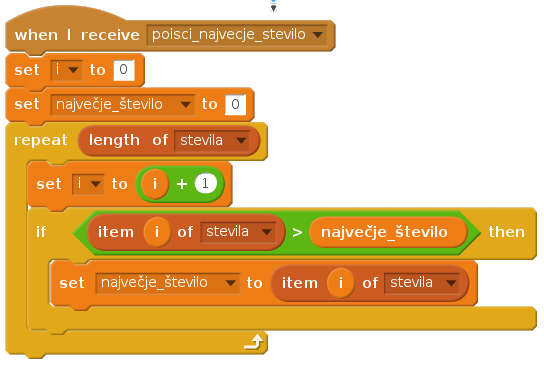
\includegraphics [width=0.6\linewidth, keepaspectratio =
    1] {./images/scratchImg/01-Scr_Alg-NajvecjeSt-img_trs.png}
    % \caption{Test}
    % \label{fig:scr:01-Alg_najdiNajvecje}
%\end {figure}

Podprogram v \textbf{Pythonu}:

\begin{lstlisting}[language=Python]
def najdiNajvecjeStevilo(seznam):
    """Funkcija poisce najvecje stevilo v seznamu."""
    i = 0
    najvecje_stevilo = 0
    for i in range(len(seznam)):
        if seznam[i] > najvecje_stevilo:
            najvecje_stevilo = seznam[i]
    return najvecje_stevilo
\end{lstlisting}
\end{examplebox}

\subsubsection{Programiranje in kodiranje}
\label{sec:programiranje_kodiranje}

Izraz programiranja smo že spoznali. Veliko krat slišimo tudi izraz,
\textbf{``kodiranje'' (\emph{ang. coding})}. Povedali bi lahko da
izraz pomeni, pisanje programske kode, konček izdelek, tisto kar na
koncu damo \textbf{prevajalniku}, kar je \textbf{izvorna koda}, da
prevede v \textbf{strojno kodo}, katero lahko potem zaganjamo.

Za vsakim programiranjem stoji seveda nek programer, lahko bi rekli,
da je za vsakim kodiranjem nekdo, ki mu pravimo
\textbf{koder}. Programer in koder stav veliko krat, dana v isti koš,
vendar si to čisto ne zaslužita, saj je programer, nekdo ki načrtuje
rešitve, na različne načine in z razčličnimi orodji preden sploh
zapiše kaj programske kode. Koder po drugi strani je tista oseba, ki
se dobro spozna na programske jezike vendar, dela veliko krat po
načrtu programera, je tisti ki na kocu zapiše rešitve in je pri tem
zelo unčikovita. Čeprav se ta dva poklica zelo povezana in so meje med
njima tudi veliko krat zabrisane sploh, če je programer in koder ena
in ista oseba \cite{web:coder}.

Pri samem poučevanju računalništva, lahko menimo, da je v prvi vrsti
pomembno to, da se učimo strategije reševanja problemov, mora
obstajati težnja kako poučevati, da bo čim več učencev postalo dobrih
programerjev in samo koderjev.

\subsubsection{Urejevalnik besedil}
\label{sec:urejevalnik_besedil}

Dober urejevalnik besedi lahko programerju lajša delo s številnimi
zmožnostmi. Opisali smo nekatere, saj nam bodo te pomagale lažje
prepoznati dober urejevalnik besedil.

%Podrobneje opiši zmožnosti urejevalnika besedil.

\begin{itemize}
\item \textbf{Barvanje rezerviranih besed prog. kode.} je značilno za
  skoraj vsak novo dobni urejevalnik besedil. Z različnimi barvami je
  olajšano branje programske kode.
\item \textbf{Samodejno zamikanje vrstic programske
    kode}. Urejevalnik, ki ima to zmožnost zna prepoznati, ko sledi
  nov del programske kode, ki je zamaknjen npr. za stavkom
  \texttt{if/else}.
\item \textbf{Ponujanje predlog za samo dokončevanje rezerviranih
    besed in funkcij prog. jezika}. Ob pisanju programske kode
  urejevalnik ponuja dokončevanje programske kode.
\item \textbf{Izpis opisa funkcij z atributi}. 
\item \textbf{Samodejno zaključevanje oklepajev}. Odprti oklepaj se
  samodejno zaključi z zaprtim in smernik za pisanje se postavi v
  sredino med oba oklepaja. 
\end{itemize}

\subsubsection{Integrirano razvojno okolje}
\label{sec:integrirano-raz-okolje}

Del \textbf{integriranega razvojnega okolja} (\textbf{IRO})
(\emph{ang. Integrated development environment \textbf{IDE}}) je dober
urejevalnik besedil, kot smo ga opisali v prejšnjem poglavju. Za IRO
je značilno, da omogoča \textbf{pisanje, testiranje, razhroščevanje}
in \textbf{prevajanje končnega programa}. Omogočajo povezavo med
datotekami projekta in knjižnicami. Svoje zmožnosti nadgrajujejo s
številnimi zunanjimi orodji, ki jih navadno vklopimo preko
vtičnikov. Slabost IRO je ta da so veliki programski paketi, ki včasih
znajo biti okorni in počasni. Pri nekaterih obsežnih IRO je tudi čas,
ki ga potrebujemo, da se ga naučimo uporabljati dolgotrajen.

\subsection{Programske paradigme}
\label{sec:programske_paradigme}

Paradigma je način kako obravnavamo in gledamo na stvari, je okvir v
katerem leži naša interpretacija realnosti sveta. Paradigma
najpogosteje pomeni vzorec delovanja v znanstvenem ali drugem
raziskovanju.  Izraz programske paradigme je več pomenka, ki povzema
mentalne procese, strategije reševanja problemov, povezave med
različnimi paradigmami, programske jezike, stil programiranja in še
več \cite{wiki:paradigme} \cite{guideTCS}.

%//Glavna definicija.
Programske paradigme so hevristike, ki se uporabljajo za reševanje
problemov. Programska paradigma analizira problem, čez specifičen
pogled in na ta način formulira rešitev za dani problem, ki ga razdeli
na manjše dele med katerimi definira razmerja.

Programske paradigme so na primer proceduralno, objektno orientirano,
funkcijsko, logično in istočasno programiranje. V nadaljevanju
spoznamo značilnosti programske paradigme objektnega programiranja,
saj je ta v zadnjih dve desetletjih najbolj razširjena. 

\subsubsection{Objektno orientirano programiranje}
\label{sec:objektno_orijentirano_programiranje}

%V objektno orientiranem \textbf{OO} pristopu programer raz

V objetno orientirano \textbf{OO} programiranje je način kako
programerji razmišljajo o svojem delu. Princip OO model realnosti
sveta predstavlja v \textbf{razredih \emph{ang. class}}. Z takim
načino zapisa programske kode je ramišljanje o programu dosti bolj
naravno \cite{shaums}.

Objekt je predstavnik različnih stvari, ki jih želimo predstavljati v
programskem razredu. Te stvari so lahko kar koli, od realnih objektov
in vse do konceptov. Podajmo primer objekta mačke. Mačka ima številne
karakteristike, kot so barva, ime, teža \dots, tem lastnostim pravimo
da so lastnosti objekta. Mačka je živo bitje, zato njenemu početju,
kot je mjavkanje, spanje, igranje \dots, pravimo, da so metode
objekta. Pri objetih lahko uporabimo analogijo in objekte poimenujemo
z samostalniki, metode so glagoli in vrednosti lastnosti objekta so
pridevniki. V nadaljevanju si bomo ogledali nekatere značilnosti, ki
definirajo programski jezi kot OO \cite{OO-JS}.

\begin{description}
\item[Razred (\emph{ang. Class}):] V resničnem življenju lahko objekte
  združujemo po nekih določenih kriterijih. Orel in sinička sta oba
  ptiča, zato jih lahko damo skupaj v razred katerega poimenujemo
  Ptiči. Razredi so načrti ali recepti za objekte, tako lahko
  ustvarimo več objektov iz istega razreda, saj je razred le shema.
\item [Enkapsulacij (\emph{ang. Encapsulation)}:] je koncept ,ki
  predstavlja, da so podatki, torej \emph{lastnosti} objektov in
  opravila, ki jih lahko opravljajo ali \emph{metode} objektov,
  združeni.
\item [Združevanje (\emph{ang. Aggregation}):] pomeni, da lahko več
  objektov združimo v en objet. To predstavlja močno orodje pri
  razčlenjevanju problemov na manjše pod probleme.
\item [Dedovanje (\emph{ang. Inheritance}):] je eleganten način kako
  porabimo eno kodo več krat. Podajmo primer, imamo splošen razred
  Oseba, ta ima lastnosti kot je ime, datum rojstva in ima napisane
  metode, ki prestavljajo funkcionalnost kot je, da Oseba lahko
  govori, hodi, je, spi. Zatem bi želeli bolj specifičen razred ko je
  Programer. Lahko bi vso kodo ponovno napisali in ji dodali
  specifično za programerja. Dedovanje omogoča, da povemo da Programer
  deduje od razreda Osebe in si tako prihranimo velik del dela.
\item [Polimorfizem (\emph{ang. polymorphisem}):] je način kako lahko
  isto ime metode uporablja več različnih razredov in posledično
  objektov ne glede nato, da je najverjetneje koda v njem
  različna.
\end{description}

Programsko paradigmo OO programiranja smo povzeli na kratko, da bi
lažje razumeli zakaj je ta programska paradigna tako popularna. V
nadaljevanju bomo spoznali, da je večina programskih jezikov, ki se
uporabljajo dan danes OO ali vsaj vsebijejo nekaj lasnosti OO
programskih jezikov.

\subsection{Programski jeziki}
\label{sec:programski_jeziki}

V tem poglavju bomo povzeli osnovne značilnosti posameznih programskih
jezikov.  Če na spletu v spletnem iskalniku podamo zahtevo
po najpopularnejšuh programskih jezik, dobimo podobne rezultate
večih spletnih strani\footnote{Pridobljeno 27.04.2016 iz,
  \url{http://www.tiobe.com/tiobe_index}.}  \footnote{Pridobljeno
  27.04.2016 iz, \url{http://githut.info/}.}\footnote{Pridobljeno
  27.04.2016 iz, \url{http://pypl.github.io/PYPL.html}.}  in sicer: \textbf{JAVA,
  C, C++, Python, C\#} v top 10 za nas pomembne najdemo še
\textbf{Java Script}. % in \textbf{Ruby}.

Programski jeziki v izobraževanju so se skozi zgodovino menjavali,
tako kot se je rezvijala računalniška znanost, kar smo že povzeli v
poglavju \ref{sec:zgodovina_programskih_jezikov}. Zanima nas, kateri so
prograsmki jeziki, ki so najbolj primerni za uporabo učenja
programiranja in se uporabljajo danes.

Vsak programski jezik bomo z kratim primerom tudi predstavili z
primerom programske, kode tako bomo dobili lažjo predstavo kakšna je
osnovna razlika v sintaksi.

Večina od zgoraj naštetih programskih jezikov je \textbf{OO} razen
izjeme \textbf{C}-ja, ki je predhodnik \textbf{C++}.  Za nas bodo z
izobraževalnega vidika zanimivi predvsme tisti, ki se uporabljajo pri
splošnem izobraževanju pri nas.

%Podajmo še razliko med programsimi jeziki, ki so za večnamesko uporabo
%in tistimi, ki jim pravimo, da imajo ožjo uporabnost.

%Razlika med prevajanimi in tolmačenimi prog. jeziki
%Uredi ker je zmazek

%% Napiši še kaj o generacijah programskih jezikov.

\subsubsection{Java}
\label{sec:pj:JAVA}

Java je več namenski programski jezik, njegova osnov so \emph{razredi}
in je OO. Njegova glavna prednost je, da napisano kodo lahko zaganjamo
ne glede na platformo na kateri teče, torej so napisani programi
neodvisni od operacijskega sistema, ki ga poganja računalnik. Zato je
za vsako platformo prilagojen \textbf{virtualni stroj za Javo}
  \emph{(ang. Java Virtual Machin \textbf{(JVM)}}, ki prevedeno kodo
poganja. Sintaksa programskega jezika je zelo podobna
\textbf{C++}. Popularnost programskega jezika je še izboljšal zaradi
operacijskega sistem za tablice in telefone \textbf{Android}, ki prav
tako teče na različici (JVM) oz so programi napisani v Javi
\cite{wiki:java}.

V izobraževanju je Java postala zelo priljubljena, prav zaradi
zmožnosti, poganjanja programov na različnih platformah. Uporablja se
na primarnem področju izobraževanja, predvsem na srednjem in visokem
šolskem področju. V sekundarnem področju izobraževanj se je uporabila
predvsem za pisanje programske opreme, ki dopolnjuje izobraževanje,
kot so fizikalne simulacije (\emph{fizleti}) in podobno. Eden od
razlogov, da se je Java na tem področju dobro uveljavila je tudi ta,
da omogoča zagon aplikacije s spletnega brskalnika, vendar je za to
potrebna instalacija posebnega vtičnika, ki to omogoča. Primer
\ref{prog:java01} prikazuje sintakso \emph{"Dobrodošel svet"}
napisanega v Javi.
%Ali moram podati referenco za te Hello world programe.
%http://www.programmingsimplified.com/java-source-codes
\begin{examplebox}[label={prog:java01}]{Program napisan v javi}
\begin{lstlisting}[language=Java]
class First {
   public static void main(String[] arguments) {
     System.out.println("Dobrodosel svet!");
  }
}
\end{lstlisting}
\end{examplebox}

\subsubsection{C++}
\label{sec:pj_c++}

C++ je vse namenski programski jezik, ki je OO in je bil zasnovan kot
sistemski programski jezik. Večina operacijskih sistemov je danes
napisana v kodi C++ in predhodniku C. Kodo programskega mora prevesti
prevajalnik preden jo lahko zaganjamo, za vsako platformo moramo
prevajati posebej.  C++ velja za najhitrejši programski jezik, z njim
lahko opravljamo tako naloge, kot je neposreden nadzor nad
polnilnikom, kot tudi vse višje funkcije, ki jih omogoča. Zato velja
za enega težje učljivih programskih jezikov. Programiranje v C++ se
uči predvsem na višjem in univerzitetnem izobraževalnem nivoju \cite{wiki:cpp}.

%https://en.wikibooks.org/wiki/C%2B%2B_Programming/Examples/Hello_world
\begin{examplebox}[label={prog:cpp01}]{Program napisan v C++}
\begin{lstlisting}[language=C++]
// 'Hello World!' program
#include <iostream>

int main()
{
  std::cout << "Hello World!" << std::endl;
  return 0;
}
\end{lstlisting}
\end{examplebox}

\subsubsection{Java Script}
\label{sec:pj_JS}

\textbf{Java Script (JS)} se je razvil z potrebe po bogatejših in dinamičnih
spletnih straneh. Začetek spleta so predstavljali statični dokumenti,
ki so bile povezane z hiper povezavami. Skirptni jezik z imenom Java
script se je prvič pojavil z spletnim brskalnikom \emph{Netscape
  2.0}. Takrat je bilo možno vstavljanje kratkih odsekov kode, ki so
spletne strani naredile dinamične. Težnja po standardizaciji
skriptnega jezika se je pojavila ko se je na trgu pojavil
\emph{Internet explorer 3.0}, saj je ta imel svojo različico sriptnega
jezika \emph{JScript}. Sedaj se standardni jezik imenuje \textbf{ECMA
  Script} oz. točneje \textbf{ECMA-262}, ki opisuje glavne dele
programskega jezika JavaScript brez specifikacij, spletnega
brskalnika \cite{OO-JS}.

Če smo v prejšnjih poglavjih govorili, da sta bila \textbf{Java} in
\textbf{C++} večnamenska jezika, je JS bil eden tistih, ki so tekli
znotraj vgrajenega gostiteljskega okolja, kot je spletni
brskalnik. Danes imamo tudi okolja, ki omogočajo, da JS teče na
strežnih, na namizju in mobilnih napravah. Torej, kljub zgoraj
omenjeni omejitvi, postaja prav tako večnamenski skriptni programski
jezik. V spodnjem primeru \ref{prog:js01} imamo primer programa
\emph{``Dobrodošel svet!''}, z \textbf{HTML} ogrodjem. Tako programska
kodo odpremo v spletnem brskalniku. Del skriptnega jezika se začne z
značko \texttt{<script type="text/javascript"> JS koda
  </script>}. Povejmo še to, da se koda programskega jezika ne
prevaja, temveč jo poganja \textbf{tolmač}.


%https://en.wikibooks.org/wiki/JavaScript/First_Program
\begin{examplebox}[label={prog:js01}]{Program napisan v JavaScriptu +
    HTML ogrodje}
\begin{lstlisting}[language=Html]
<!DOCTYPE html>
<html lang="en">
  <head>
    <title>Some Page</title>
    <script type="text/javascript">
      alert("Hello World!");
    </script>
  </head>
  <body>
    <p>The content of the web page.</p>
  </body>
</html>
\end{lstlisting}
\end{examplebox}

\subsubsection{Python}
\label{sec:pj_python}

\textbf{Python} je zelo pogosto uporabljen večnamenski programski
jezik. Njegovo kodo podobno kot JS poganja tolmač. Zasnovan je tako,
da je koda čim bolj berljiva in njegova sintaksa omogoča, da
programske koncepte zapišemo v čim manj vrsticah, kakor bi jih lahko v
Javi ali C++. Če so posamezni odseki ali bloki programske kode pri
Javi in C++ označeni z zavitimi oklepaji (``{}''), jih v Pythonu
označimo z tabulatorskim zamikom. V Pythonu lahko uresničimo več
programskih paradigem, kot je OO ali proceduralno
programiranje. Omogočen je dinamičen tip spremenljivk, ima urejeno
avtomatsko upravljanje z pomnilnikom in ima veliko standardno
knjižnico \cite{wiki:python}.

%Kje to piše, da je priporočljiv jezik v SŠ
Pyon se veliko uporablja tudi v izobraževalne namen. Pri nas se
priporoča za začetke učenja programskega jezika na srednjem šolskem
izobraževalnem nivoju. Zaredi tega, ga bomo v diplomskem delu
uporabljali, ko glavni demonstracijski programski jezik.

%https://en.wikibooks.org/wiki/JavaScript/First_Program
\begin{examplebox}[label={prog:py01}]{Program napisan v Pythonu
    HTML ogrodje}
\begin{lstlisting}[language=Python]
print (``Hello world!''')
\end{lstlisting}
\end{examplebox}

\subsection{Osnovni koncepti programiranja}
\label{sec:Osnvni koncepti_programiranja}

% Predstavljeni koncepti na primerih eden OŠ Scratch drugi Python.
V naslednjem odstavku se bomo vprašali kako lahko formuliramo sintakso
programskega jezika? In kaj je npr. definicija \emph{kopice}.V ta
namen definiramo mehko idejo po avtorju Hazzan \cite{guideTCS}, ki je
naslednja. Mehka ideja je koncept, ki mu ne moremo pripisati toge,
niti formalne definicije. Mehke ideje ni niti možno opisati z točno
določeno aplikacijo. Na tem mestu se postavlja vprašanje kako lahko
defineramo nekaj kar se odvija po korakih.

Da odgovorimo na zgornji dve vprašanji, lahko povemo, da so pravila
sintakse togi orisi pri pisanju programske kode in da so semantična
pravila mehke ideje. Opozorimo še na to, da koncepti v računalniški
znanosti niso le toga pravila ali samo mehke ideje, temeč skupek
obojega. V spodnji tabeli \ref{tab:koncept_spremenljivka} prikazuje
primer spremenljivke.

\begin{table}[!h]

\caption{Prikaz dvojnih, togih in mehkih orisov idej na primeru
  spremenljivke \cite{guideTCS}. }
\label{tab:koncept_spremenljivka}
\begin{tabular}{
  | p{0.30\linewidth-2\tabcolsep} |
  p{0.30\linewidth-2\tabcolsep} |
  p{0.40\linewidth-2\tabcolsep} | }
  \hline
  \rowcolor{sbase01!100}
  & \textbf{togi orisi} & \textbf{mehki orisi}\\
  \hline
  ime spremenljivke & Pravilo sintakse. & Potreba po imenu
                                          spremenljivke. Katero ime
                                          spremenljivke je pomembno in
                                          zakaj ga je potrebno
                                          določiti.\\
  \hline
  vrednost spremenljivke & Pravila tipa spremenljivke. Rezervacija
                           pomnilnika. & Spremenljivka ima eno
                                         vrednost, ki se lahko
                                         spreminja s časom.\\
  \hline
  dodelitev začetne vrednosti & Pravila sintakse. & Pomen dodelitve
                                                  začetne vrednosti\\
  \hline

\end{tabular}
\end{table}

V nadaljevanju bomo pregledali in skušali razložiti osnovne koncepte
pri programiranju. Z primerom bomo pokazali enega izmed načinov, kako
jih prestavimo. Za vodilo bomo uporabili učni načrt za OŠ, ki smo ga
pregledali v poglavju \ref{sec:neobvezno_izbirni_predmet_rac} in SŠ,
ki je v poglavju \ref{sec:Programiranje_v_SŠ}. Primeri programov, ki
jih bomo uporabljali in prilagodilo so povzeti s knjige in spletne
strani \emph{``Learning python the hard way''} \cite{web:PTHardWay}.


%%Lahko podamo primere programov z problemskim navodilom in rešitvijo
%%v Pythonu in Scratchu, kjer je to možno.
\subsubsection{Izpis in računske operacije}
\label{sec:izpis_rac_operacije}

Osnovno interakcijo z računalnikom lahko opišemo na naslednji
način. Računalniku damo neke vhodne podatke, ta podatke po navodilu
programa obdela in nam poda rezultate na neko izhodno naprava. Ta
izhodna naprava je na primer zaslon in na njem se izpisujejo obdelani
podatki. Izpišimo nekaj stavkov, pri tem uporabljamo ukaz
\texttt{print}.

\begin{examplebox}[label={prog:izpis}]{Izpis besedila na zaslon |
    \texttt{01\_izpis\_na\_zaslon.py} \cite{web:PTHardWay}}
  \textbf{Navodilo naloge:} Sledi navodilu, ki je zapisano v programski
  kodi.
\rule{\textwidth}{.4pt}
\begin{lstlisting}[language=Python]
#Del programa, ki nocemo, da ga uposteva tolmac,
#oznacimo z # in ga imenujemo komentar.
print "Pozdravljeni, to je nas prvi izpis na zaslonu."
print "Izpisemo lahko tudi pravzno vrstico. \n"
#Za izpis prazne vrstive uporabimo "\n"
print "Pred to vrstico je prazna! in za njo.\n"
\end{lstlisting}
\tcblower
\begin{Verbatim}[fontsize=\footnotesize]
$ python 01_izpis_na_zaslon.py
Pozdravljeni, to je nas prvi izpis na zaslonu.
Izpisemo lahko tudi pravzno vrstico.

Pred to vrstico je prazna! in za njo.
\end{Verbatim}
\end{examplebox}

Ena izmed glavnih nalog računalnikov so računske operacije, zato si
poglejmo dva primera izračunov v programskem jeziku Python.

\begin{examplebox}[label={prog:racunske_operacije}]{Računske operacije |
    \texttt{02\_racunske\_operacije.py} \cite{web:PTHardWay}}
  \textbf{Navodilo naloge:} Sledi navodilu, ki je zapisano v programski
  kodi.
\rule{\textwidth}{.4pt}
\begin{lstlisting}[language=Python]
#Izračunajmo nasednje izrazein izpišimo njiho rezultat.
#Preden poženemo program izračunajmo vrednost sami.
print 100 - 5%2 + 3*4 - 22/3
print 4+7 > 13
\end{lstlisting}
\tcblower
\begin{Verbatim}[fontsize=\footnotesize]
$ python 02_racunske_operacije.py
104
False
\end{Verbatim}
\end{examplebox}

\subsubsection{Spremenljivke}
\label{sec:spremenljivke}

V tem poglavju bomo uresničili naslednje cilje vendar smo jim nekoliko
spremenili vrstni red:
\begin{itemize}
\tightlist
\item \textbf{znajo izpisovati vrednosti spremenljivk med izvajanjem programa
  in izpisati končni rezultat},
\item \textbf{znajo spremenljivkam spremeniti vrednost s prireditvenim
  stavkom},
\item \textbf{znajo v program vključiti konstante in spremenljivke},
\item \textbf{ razumejo različne podatkovne tipe in jih znajo uporabiti v
  programu},
\item \textbf{znajo v programu prebrati vhodne podatke in jih vključiti v
  program},
\end{itemize}

Spremenljivke so način kako shranjujemo podatke v računalniku.  Ime
spremenljivke ima podobno vlogo kot imena ljudi ali stvari v
vsakdanjem življenju. Ljudje in stvari imajo imena zato, da si jih
lažje zapomnimo in se z njimi in o njih lažje pogovarjamo. Podobno je
to v programiranju, izbrati si moramo dobra imena spremenljivk, saj
bomo tako lažje brali napisano kodo. Poglejmo primer
\ref{prog:spremenljivke}.

\begin{examplebox}[label={prog:spremenljivke}]{Izpis besedila na
    zaslon | \texttt{03\_uporaba\_spremenljivk.py} \cite{web:PTHardWay}}
\textbf{Navodilo naloge:}

Na parkirišču je 100 avtomobilov, vsak izmed avtomovilov ima 5
sedežev. Z temi avtomobili želimo pripeljati 90 potnikov od tega jih
ima 30 vozniško dovoljenje. Izračunaj in izpiši naslednje podatke.
\begin{itemize}
\item Koliko avtomobilov je navoljo.  Koliko šoferjev je navoljo?
\item Koliko avtomobilov bo ostalo na parkirišču, če bodo vozili vsi
  šoferji?
\item Koliko ljudi lahko prepeljemo z vsemi avtomobili?
%\item Koliko avtomobilov bomo uporabili, da pripeljemo vse potnike?
\item Kakšno je povprečno število potnikov, če vozijo vsi vozniki?
\end{itemize}
\rule{\textwidth}{.4pt}
\begin{lstlisting}[language=Python]
#1. Določimo spremenljivke:
avtomobili = 100
prostor_v_avto = 5.0
potniki = 90
soferji = 30
#2. Izračunajmo vrednosti in jih shranimo v spremenljivke:
avtomob_na_park = avtomobili - soferji
kapac_avtomob = avtomobili * prostor_v_avto
avtomob_na_potnikov = potniki/prostor_v_avto
povpr_st_potnikov = potniki/soferji
#3. Izpišimo vse zahtevane podatke.
print ("Na voljo je", avtomobili, "avtomobilov.")
print ("Na voljo je", soferji, "šoferjev.")
print ("Na parkiriscu bo ostalo",avtomob_na_park, "avtomobilov.")
print ("Z vsemi avtomobili prepeljemo", kapac_avtomob, "potnikov.")
print ("Povpr. st. potnikov je",povpr_st_potnikov, ",ce vozijo vsi soferji.")
\end{lstlisting}
\tcblower
\begin{Verbatim}[fontsize=\footnotesize]
$ python 03_uporaba_spremanljivk.py
Na voljo je  100 avtomobilov.
Na voljo je  30 šoferjev.
Na parkiriscu bo ostalo  70 avtomobilov.
Z vsemi avtomobili lahko prepeljemo  500.0 potnikov.
Povprecno stevilo potnikov je  3, ce vozijo vsi soferji.
\end{Verbatim}
\end{examplebox}

\subsubsection{Pogojni stavki in vejitve}
\label{sec:pogojni_stavki_vejitve}

V tem poglavju bomo uresničili naslednje cilje: \textbf{znajo
  uporabiti pogojni stavek in izvesti vejitev}.

\begin{examplebox}[label={prog:pogojni}]{Program odločitve |
    \texttt{05\_pogojni\_stavki.py} \cite{web:PTHardWay}}
\textbf{Navodilo naloge:}
Kodo programa spremeni tako, da boo potniki potovali z avtomobili. 
\rule{\textwidth}{.4pt}
\begin{lstlisting}[language=Python]
potniki = 40
avtomobili = 40
if avtomobili > potniki:
    print ("Pojdite z avtomobili.")
elif avtomobili < potniki:
    print ("Ne morete z avtomobili.")
else:
     print ("Ne morem se odločiti.")
\end{lstlisting}
\tcblower
\begin{Verbatim}[fontsize=\footnotesize]
$ python 05_pogojni_stavki.py
Ne morem se odločiti.
\end{Verbatim}
\end{examplebox}

\subsubsection{Zanke}
\label{sec:zanke}

V tem poglavju bomo uresničili naslednje cilje: \textbf{razumejo pojem zanke
in ga znajo uporabiti za rešitev problema}.

\begin{examplebox}[label={prog:zanka}]{Zanka |
    \texttt{06\_zanka.py} \cite{web:PTHardWay}}
  \textbf{Navodilo naloge:}
  Napišite zanko, ki pregleda seznam in prešteje in izpiše vsa liha
  števila.
\rule{\textwidth}{.4pt}
\begin{lstlisting}[language=Python]
#Podan seznam celih stevil.
cela_st = [11, 41, 2, 32, 12]
vsota_lihih = 0
for st in cela_st:
    if st%2 == 1:
        print (st)
        vsota_lihih += 1
print ("Vseh lihih stevil:", vsota_lihih)
\end{lstlisting}
\tcblower
\begin{Verbatim}[fontsize=\footnotesize]
$ python 06_zanka.py
11
41
Vseh lihih stevil: 2
\end{Verbatim}
\end{examplebox}

%\subsubsection{Kompletksi tipi podatkov}
%\label{sec:kompleksni_tipi_podatkov}
%
%V tem poglavju bomo uresničili naslednje cilje:
%\begin{itemize}
%\item \emph{razumejo kompleksnejše tipe podatkov (nizi,
%    seznami/tabele) in jih znajo uporabiti v programu},
%\end{itemize}

%Preostali cilji z OŠ so še naslednji!
% \item \emph{razumejo kompleksnejše tipe podatkov (nizi, seznami/tabele) in
%   jih znajo uporabiti v programu},
% \item \textbf{prepoznajo in znajo odpraviti napake v svojem programu},
% \item \emph{znajo popraviti napako v tujem programu},
% \item \emph{znajo spremeniti program, da dosežejo nov način delovanja
%   programa},
% \item \emph{znajo rezultate naloge zapisati v datoteko},
% \item \textbf{se seznanijo z dogodkovnim programiranjem},



%%% Local Variables:
%%% mode: latex
%%% TeX-master: "../diploma"
%%% End:

\newpage
\section{Pristopi in strategije poučevanja}
\label{sec:aktivno_resevanje_prob}

V naslednjem poglavju raziščemo, kaj so sodobni pristopi in značilne
strategije pri poučevanju računalniške znanosti in
programiranja. Izpostavili bomo \textbf{model aktivnega učenja} in
\textbf{strategijo reševanja problemov}. Z razumevanjem tega bomo v
nadaljevanju lažje ocenili ali uporaba spletnih portalov vzpodbuja oba
pristopa.

\subsection{Model aktivnega učenja}
\label{sec:model-aktivn-uenja}

Vsak pouk računalništva naj bi imeti modelno zgradbo in bi upošteval
naslednja načela:
\begin{itemize}
\tightlist
\item naj vzpodbuja študente s pozitivno naravnanim poukom in jim naj
  omogoča okolje kjer najdejo pomoč.
\item Pouk računalništva je naj grajen na konstruktivnih metodah
  poučevanja in aktivnem učenju.
\end{itemize}

\textbf{Konstruktivizem} je kognitivna teorija, ki preučuje naravo
procesov učenja. Po tem principu naj bi učenci konstruirali novo
znanje na osnovi preurejanja in izpopolnjevanja že obstoječega
znanja. Znanje se gradi na obstoječih mentalnih strukturah in na
odzivu, ki ga dobi učenec iz učnega okolja. Mentalne strukture so
grajene korak za korakom, ena za drugo, seveda s to metodo lahko pride
tudi do sestopanja ali slepih koncev. Proces je povezan z Piagetovim
mehanizmom asimilacije \cite{guideTCS}.

Pri \textbf{aktivnem učenju} je najpomembnejše to, da učenci z lastno
aktivnostjo ugotovijo, sami za sebe kako nekaj deluje. Sami si morajo
izmisliti primere, preiskusiti lastne veščine in reševati neloge, ki
so jih že ali jih še podo spoznali. Učenje je aktivno usvajanje, je
gradnja idej in znanja. Za učenje mora biti posameznik aktivno
vključen v gradnjo svojih lastnih mentalnih modelov.  Model aktivnega
učenja je sestavljen s štirih korakov \cite{guideTCS}.

\begin{itemize}
\tightlist
\item \textbf{Sprožilec} Je je naloga, ki predstavlja iziv za uvod v novo
tematiko.
\item \textbf{aktivnost} Študenti izvajajo aktivnost, ki jim je bila
predstavljena v sprožilcu. Ta kora je lahko kratek ali lahko
zavzame večju del učne ure. To je odviso od vrste sprožilca in
izobraževalnih ciljev.
\item \textbf{diskusija} sledi po koncu aktivnosti, kjer se zbere zeloten
razred, neglede na obliko dela. V temo koraku študenti izpopolnijo
koncepte in ideje, kod del konstruktivnega učnega procesa.
\item \textbf{povzetek} je lahko izračen v različnih oblikah, kot so
zaokrožene definicije, lahko so miselni vzorci ali povezav med
temami, ki so jih obravnavali študenti in med drugimi temami, ki se
navezujejo nanje.
\end{itemize}

Ko se ta model izkaže za primernega, ga lahko uporabimo v številnih
učnih urah v različnih variacijah. Zanima nas ali znajo pristop
aktivnega učenja spletni portali upoštevati?

\subsection{Strategije reševanja problemov}
\label{sec:strategije_reševanja_problemov}
%Preveriti moram knjigo Norbert Jaoušovec
Programiranje je preces pri katerem rešujemo probleme, zato je
reševanje problemov v središču poučevanja računalniške
znanosti. Reševanje problemov je zahteven mentalni proces. Če na
spletu pobrskamo za strategije reševanja problemov lahko hitro
ugotovimo na obstajajo različne strategije. Med njimi lahko najdemo
različne kot je \textbf{abstrakcija, analogija, brainstorming, deli in
  vladaj} in mnoge druge \cite{book:jausovec}. Proces in tehnike
reševanje problemov se uporablja v mnogih tehničnih in znanstvenih
disciplinah \cite{guideTCS}.

V nekaterih primerih učenci sami razvijejo strategijo s katero rešijo
nek problem. Otroci si na primer sami izmislijo enostvno seštevanje in
odštevanje, dolgo pred tem kadar se to učijo pri pouku
matematike. Toda brez formalne podpore za učin2Akovito strategijo
reševanja problemov, spodleti še tako inovativnemu učencu tudi pri
enostavnih strategijah kot je \textbf{preizkus in napaka}. Zato je
pomembno, da se uči strategij za reševanje problemov.

%\subsection{Proces reševanja problemov}
%\label{sec:proces_reševanja_problemov}

Vsak osnoven proces, ki se ukvarja z reševanjem problemov, ne glede na
znanstveno disciplino, se začne z opisom problema. Vsak problem se
navadno zaključi z neko rešitvijo, ki je v nekaterih primerih izražena
z \textbf{zaporedjem korakov} ali \textbf{algoritmom}. V računalnik
algoritem zapišemo z kodo nekega programskega jezika. Zapisan
algoritem testiramo tako, da kodo prevedemo v strojni jezik in jo
izvedemo. Za pravilno delovanje programa primerjamo vhodne in željene
izhodne podatke. Preden pridemo od opisa problema do podane rešitve
moramo prehoditi kar nekaj težkih korakov. Na te vmesne korake lahko
gledamo kot na procese odkrivanja, zato lahko na reševanje problemov
gledamo tudi kot na kreativen, umetniški proces. Splošno priznani
koraki reševanja procesov so naslednji \cite{guideTCS}:

\begin{enumerate}
\tightlist
\item \emph{Analiza problema}. Najprej je pomembno da razuemo kaj je
  problem in ga znamo identificirati. Če tega ne znamo, ne moremo
  priti do nobene rešitve.
\item \emph{Alternativnie rešitve}. Razmišljamo o alternativnih
  rešitvah kako bi lahko rešili nek problem.
\item \emph{Izbira pristopa}. Izberemo primeren pristop, kako rešiti problem.
\item \emph{Razgradnja problema}. Problem razgradimo na manjše podprobleme.
\item \emph{Razvoj algoritma}. Algoritem razvijamo po korakih, ki smo
  jih določili v podproblemih.
\item \emph{Pravilnost algoritma}. Preverjanje pravilnosti algoritma.
\item \emph{Učinkovitost algoritma}. Izračunamo učinkovitost algoritma.
\item \emph{Refleksija}. Naredimo refleksijo in analizo na pot, ki smo
  jo naredili pri reševanju problema in naredimo zaključek z tem kar
  lahko izboljšamo za naslednji problem, ki ga bomo reševali.
\end{enumerate}

Točen recept kako se lotiti reševanja ne obstaja. Učencem lahko le
pokažemo nekatere metode in strategije, ki jim lahko pomagajo pri
reševanju problemov. Da bi bolje znali oceniti, kako izrazito spletni
portali upoštevajo korake strategije reševanja problemov, poglejmo še
nekatere pomembne korake podrobneje in koko se z njimi spopadajo
novinci.

%Od tu naprej je mogoče prepodrobno in ni potrebno vsega spodnjega.

\subsubsection{Razumevaje problema}
\label{sec:razumevanje problema}

Razumevanje problemov je prva stopnja v procesu reševanja
problemov. Pri reševanju algoritemskih nalog najprej moramo
prepoznati, kaj so vhodni podatki in kateri podatki naj bi bili
izhodni. Če znamo povedati kaj bodo vhodni podatki, razumemo tudi
bistvo samega problema.

\subsubsection{Načrtovanje rešitve}
\label{sec:načrtovanje_rešitve}

Novinci se spopadajo z največjimi težavami na začetni stopnji
načrtovanja rešitve za nek problem. V nadaljevanju so predstavljene
tri strategije, ki jih lahko uporabimo na tem koraku reševanja
problema.

\begin{description}
\item [Definicija spremenljivk problema:] Pri rešitvi problema
  si pomagamo tako, da ugotovimo kaj morajo biti vhodni in kateri bojo
  izhodni podatki. S tem razjasnimo problem. V naslednjem koraku
  definiramo \textbf{spremenljivke}, ki so potrebne za rešitev
  problema.
\item [Postopno izboljševanje (\emph{ang. Stepwise
      Refinement)}:]Po tej metodi nas najprej zanima celoten pregled
  strukture problema in odnosi med posameznimi deli. Zatem se šele
  poglobimo specifični in kompleksni implementaciji posameznih pod
  problemov. Postopno izboljševanje je metodologija, ki poteka od
  \textbf{zgoraj-navzdol}, torej od splošnega k specifičnemu. Drugačen
  pristop je od \textbf{spodaj-navzgor}. Za oba pristopa velja da eden
  drugega dopolnjujeta. V obeh primerih je problem razdeljen na manjše
  pod probleme ali naloge. Glavna razlika med obema je mentalni
  proces, ki je potreben za en ali drugi pristop.  V nadaljevanju se
  posvetimo samo pristopu od \textbf{zgoraj-navzdol}. Rešitev, ki jo
  poda \textbf{postopno izboljševanje} ima modularno obliko, ki jo:
  \begin{enumerate}
    \tightlist
  \item jo lažje razvijamo in preverjamo,
  \item jo lažje beremo in
  \item nam omogoča, da uporabljamo posamezne pod rešitve tudi za
    reševanje drugih problemov.
  \end{enumerate}
\item [Algoritemski vzorci:] Algoritemski vzorci združujejo
  matematični pogled in elemente načrtovanja. Vzorec podaja načrt na
  rešitev, s katero se srečamo mnogokrat. Algoritemski vzorci so
  primeri elegantnih in učinkovitih rešitev problemov in predstavljajo
  abstraktni model algoritemskega procesa, katerega lahko prilagodimo
  in ga integriramo v rešitve drugim problemom.

  Pri tem procesu lahko nastopi težava prepoznave vzorca algoritma pri
  novincih, saj ti niso sposobni prepoznati podobnosti med posameznimi
  algoritmi ali ne znajo prepoznati bistvo problema, njihove posamezne
  komponente in razmerja med njimi, da bi lahko rešili nove
  probleme. V takih primerih novinci radi ponovno izumijo že njim
  poznane rešitve, ki bi jih lahko uporabili. Te težave navadno
  nastanejo zaradi slabe organizacije sistematike znanja o algoritmih.

  Proces reševanja problemov z algoritemskim vzorcem se navadno začne
  z prepoznavanjem komponent, ki vodijo k rešitvi in iskanjem podobnih
  problemov, na katere še imamo znane rešitve. Zatem prilagodimo
  vzorec prilagodimo za rešitev problema in ga vstavimo v celotno
  rešitev. V večini primerov je potrebno vstaviti več različnih
  vzorcev, da dobimo neko novo rešitev.
\end{description}

\subsubsection{Preverjanje rešitve}
\label{sec:preverjanje_rešitve}
Ko imamo pripravljeno rešitev moramo preveriti ali je ta
pravilna. Pogled na preverjanje pravilnosti rešitve je lahko
teoretične in praktične narave. Razhroščevanje (\emph{ang. debugging})
spada me vrsto aktivnosti, ki nam pomaga pri ugotavljanju pravilnosti
rešitve. Splošno velja da proces razhroščevanja, z programom, ki nam
pomaga razhroščevati (ang. debugger) ali brez njega, poglablja
razumevanje računalniške znanosti. Z tem ko učenci razmišljajo, kako
bodo preverjali ali njihov program deluje pravilno, hkrati v njih
poteka miselni proces refleksije o tem kako so implementirali določen
program in kako ga bojo morebiti morali spremeniti.

Na nivoju do srednje šole uporabljamo praktične metode ugotavljanja
pravilnosti programa, kot je razgroščevanje. Ko želimo znanje
pravilnosti delovanja poglobiti se lahko lotimo tudi teoretične
analize.

\subsubsection{Refleksija}
\label{sec:refleksije}

Refleksija je mentalni proces ali obnašanje, ki nam omogoča da neko
delovanje analiziramo in o njem tudi premislimo. Refleksija je
pomembno orodje v splošnem učnem procesu, prav tako spadam med
kognitivne procese višjega reda. Z refleksijo učenec dobi priložnost,
da stopi korak nižje in premisli o svojem razmišljanju in tako
izboljša veščino reševanja problemov. Refleksivno razmišljanje je
proces, ki zahteva veliko časa in vaje. Med procesom reševanja
problemov, lahko refleksijo uporabimo na različnih stopnjah.

\begin{itemize}
\tightlist
\item \emph{Pred} reševanjem problemom. Ko problem preberemo, in že
  načrtujemo rešitev, se splača uporabiti refleksijo in razmisliti o
  tem ali smo morda že reševali podoben problem in temu primeren
  vzorec algoritma.
\item \emph{Med} reševanjem problema. Ko rešujemo problem refleksija
  služi, kot pregled, kontrola in nadzor. Na primer, ko nastopijo
  težave pri načrtovanju rešitve ali morda zaznamo težavo ali
  napako. Temo procesu lahko pravimo \textbf{refleksija v akciji}.
\item \emph{Po} reševanju problema. Ko že najdemo rešitev, ki deluje,
  nam refleksija služi kot orodje z katerim pregledamo učinkovitost
  delovanja. Pregledamo strateške odločitve, ki so bile sprejete med
  samim načrtovanjem rešitve.
\end{itemize}

Refleksija je kreativni proces in je pomemben za učenca tako kot za
učitelj.


%%% Local Variables:
%%% mode: latex
%%% TeX-master: "../diploma"
%%% End:

\newpage
\section{Spletni portali za učenje programiranja}
\label{sec:SPUP}

Spletne portale za učenje programiranja (\textbf{SPUP}) bomo
predstavili in spoznali tako, da bomo najprej pregledali, kaj so bili
glavni razlogi, da so se pojavili. Spletni portali za učenje
programiranja, v nadaljevanju \textbf{SPUP}, so nastali takoj po
razmahu interneta v začetku novega tisočletja. Najprej so nastali na
univerzah. Zanima pa nas, kaj so glavni razlogi za nastanek SPUP.  Poleg
tehnoloških zmožnosti IKT za nastanek spletnega portala nas zanimajo
predvsem težave, ki so jih skušali premostiti z uporabo SPUP.

Spletni portali so nastali na različnih univerzah, ogledali si bomo
spletni portal, ki je nastal na \emph{Odprti univerzi v Hong
  Kongu} (\textbf{OUHK}), na \emph{Univerzi Strathclyde v Veliki
  Britaniji} (\textbf{USVB}) in \emph{Queensland University of
  Technology, Australia} (\textbf {QUTA}).

Zanimali nas bodo predmeti, ki veljajo za začetne pri poučevanju
računalniške znanosti in programiranja. \textbf{Novinci}, kot jih bomo
imenovali, so študenti, ki se šele začnejo učiti programiranja. V
diplomskem delu nas zanimajo le učenci osnovnih šol in dijaki
srednjih, vendar se oni prav tako šele srečujejo s programiranjem,
podobno kot študentje, in jih bomo zato vse poimenovali kot
\textbf{novince}.

%%OPOMBA: To trdim brez citata.
Kot je razvidno iz literature, bomo lahko sklepali na nekatere skupne
značilnosti vseh novincev, ne glede na težavnostno stopnjo, na kateri
se nahajajo, saj je programiranje veščina, ki ni dana naravno in se je
mora vsak priučiti.

%Kaj je spletni portal?

%Spletni sistem omogoča študentom in mentorjem spletno okolje za učenje
%programiran.

%Kako opredelimo kaj je to (ang. Course) ali je to en predmet, ali
%skupek predmetov.

\subsection{Razlogi za nastanek spletnih portalov}
\label{sec:razlogi_za_nastanek_SPUP}

Na Odprti univerzi v Hong Kongu (\textbf{OUHK}) ponujajo tri
računalniške sklope različnih težavnosti za dodiplomske
programe. Imajo zelo veliko populacijo študentov, ki se učijo
programiranja. Avtorji članka \cite{ITaLCP_DistanceEdu}
ugotavljajo, da je proces učenja programiranja kompleksen in zahteva
veliko vaje. Izkaže se, da praktični
del igra poglavitno vlogo v učnem procesu.

Glavna težava, s katero se srečujejo na \textbf{OUHK}, je ta, da se
število študentov, ki se vpišejo v smeri računalništva,
povečuje. Povečanje študentov pomeni manj časa za mentorstvo za
posameznega študenta.

Da bi študentje lahko normalno sledili pouku na daljavo, si morajo
doma urediti delovno okolje, kjer lahko programirajo. Študenti,
dobijo vso potrebno učno literaturo in tudi programsko opremo, ki
predstavlja \textbf{prevajalnik} in \textbf{razvojno okolje}. Izkaže se,
da imajo številni težavo nastaviti in se spoznati z integriranim
razvojnim okoljem (\emph{ang. Integrated Development Environment
  (\textbf{IDE})}) \cite{ITaLCP_DistanceEdu}.

Težave pri izobraževanju na daljavo se pojavijo tudi v
komunikaciji. Študent, ki se izobražuje od doma in naleti na neko
težavo, ki je ne zna sam rešiti, nima dostopa do svojih kolegov ali
mentorjev. Do mentorjev lahko dostopa le preko telefonskih klicev ali
elektronske pošte. Če pogledamo še s strani mentorjev, imajo ti težavo
s spremljanjem napredka velikega števila študentov.

%%Tu pride uvod z naslednjega članka!

Naslednji članek, ki so ga sestavili avtorji z \emph{Univerze
  Strathclyde iz Velike Britanije} (\textbf{USVB}), se ukvarja z
raziskovanjem vpliva nove strategije kognitivnega pristopa k
poučevanju programiranja, ki spreminja mentalni model študentom tako,
da v njih ustvari konflikt. V ta namen je bilo razvito tudi spletno
okolje, ki implementira uporabo nove kognitivne strategije
\cite{mentalModels}.

%kaj točno je mentalni model in ali je to pravi prevod

Kot pravijo avtorji v članku, s hitrim razvojem IKT narašča tudi
potreba po sposobnih programerjih in učenje programiranja postaja
globalna skrb. V prvem letu pri predmetih programiranja študenti
obvladajo naloge programiranja dosti slabše, kot bi to
pričakovali. Slaba uspešnost se pozna predvsem pri tem, da se mnogi
izpišejo s smeri računalništva, takih je kar od 30 do 50 \%. Kot
avtorji poudarjajo in povzemajo po drugih študijah, so za to v glavnem
krive težave pri reševanju problemskih nalog, ki nastopajo v
programiranju. Nekatere druge študija vidijo krivca za neuspeh tudi v
napačnem razumevanju ključnih konceptov pri programiranju, ki so lahko
posledično krivi za težave pri reševanju problemov. Tradicionalni učni
pristop je za učenje programiranja manj zanesljiv, da bi zagotovil
pravilnost v razvoju mentalnih modelov o konceptih
programiranja. Študije kažejo, da študenti po enem letu predmeta
programiranja še vedno nimajo pravih mentalnih modelov o osnovnih
programskih konceptih.

Na univerzi QUTA se pri začetnih predmetih programiranja srečujejo s
podobnimi težavami kot na OUHK in USVB.

\begin{enumerate}
\tightlist
\item Namestitev in nastavitve okolja za programiranje.
\item Uporaba urejevalnika besedil.
\item Razumevanje programskih vprašanj in uporabe sintakse jezika pri
  pisanju programske kode.
\item Razumevanje napak prevajalnika.
\item Razhroščevanje.
\end{enumerate}

Ugotavljajo, da je pri danih vajah programiranja pomembno, da ob
težavah novinci dobijo čimprajšni odziv mentorja. V velikih razredih
se to izkaže za zelo zahtevno. Tudi začetniki, ki uspešno premagajo
začetne ovire in se lotijo takojšnjega programiranja, imajo zelo slabo
napisano in konstruirano programsko kodo. Pomagati študentom pisati
kakovostno programsko kodo je prav tako časovno zelo zahtevno. Težave
programiranja se stopnjujejo, ko se za učenje progremiranja uporabljajo
OO programski jeziki, saj ti zahtevajo visoko stopnjo
abstraktnega razumevanja programskih konceptov. Za izdelavo spletnega
portala za učenje programiranja so na QUTA bili pomembni naslednji
cilji \cite{thesisAWebP}.

\begin{itemize}
\item Omogočiti lažji začetek pri učenju programiranja s pogostim
  odzivom mentorjev na težave novincev. S pomočjo ob pravem času
  spremenimo odnos novincev do programiranja.
\item Izboljšati uspeh začetnih predmetov programiranja.
\item Pomoč mentorjem pri učenju in administraciji predmetov
  programiranja.
\end{itemize}

\subsection{Primeri implementacije in sistemska arhitektura}
\label{sec:sistemska_arhitektura_All}

Zanimalo nas je tudi, kakšna je morebitna sistemska arhitektura takega
spletnega portala, zato si pomagamo s primerom arhitekture, ki so ga
izdelali na \textbf{OUHK}.  V nadaljevanju govorimo o
\emph{aktivnostih}, ki jih mora študent opraviti, to so naloge,
programske rešitve na zastavljene probleme. Študenti na \textbf{OUHK}
se učijo programiranja v programskem jeziku \textbf{Java}.

Kot prikazuje slika \ref{fig:OUHK_cmsArch}, je sistem urejanja vsebine
(\emph{ang. Contetnt Managment System (\textbf{CMS})}), teče na
spletnem strežniku \emph{\href{http://www.apache.org/}{Apache}} z
\emph{\href{https://www.mysql.com/}{MySQL}} podatkovno bazo. Sistem je
narejen iz štirih podmodulov, ki so napisani v skriptnem jeziku
\emph{\href{http://php.net/}{PHP}}.

\begin{figure}[htb!] \centering
  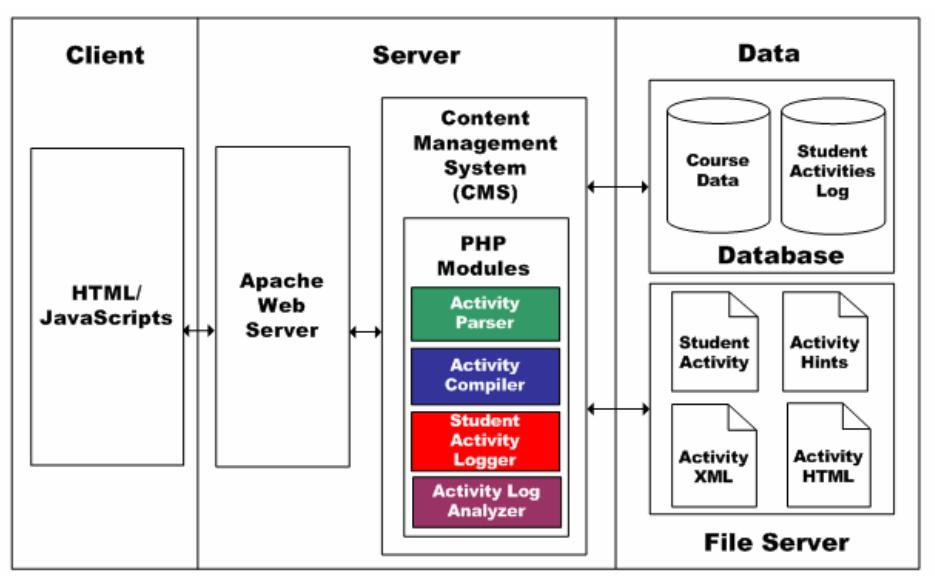
\includegraphics[width=0.9\linewidth, keepaspectratio =
1]{./images/SystemArch01_OUHK_DistanceEdu.jpg}
  \caption{Sistemska arhitektura spletnega portala za učenje
    programiranja, kot so jo naredili na OUHK \cite{ITaLCP_DistanceEdu}.}
  \label{fig:OUHK_cmsArch}
\end{figure}

Ti moduli so naslednji: zajem aktivnosti, prevajalnik aktivnosti,
dnevnik študentove aktivnosti in analizator dnevnikov aktivnosti. Samo
delovanje je naslednje: ko odjemalec pošlje zahtevo za neko aktivnost,
se ta naslovi strežniku, ki poišče programsko aktivnost. Z modulom
\emph{zajema aktivnosti} strežnik zajame aktivnost, ki je zapisana v
obliki \textbf{XML}, in naloži vse potrebne datoteke. Zajem aktivnosti
prav tako naloži študentovo predhodno delo, ki je shranjeno v datoteki
aktivnosti. Ko se vse zajame in naloži, se vsebina pošlje v obliki
\textbf{HTML} nazaj h klientu.

Strežnik omogoča tudi prevajanje aktivnosti. Ko strežnik dobi prošnjo
za prevajanje programske kode, se ta prevede, če v njej ni
sintaktičnih napak, in se ustvari datoteka \textbf{JAR}, ki jo študent
lahko prenese s strežnika. Če so v programu napake, se ustvari dnevnik
napake v trenutni aktivnosti, prav tako se napaka izpiše na zaslonu
študenta. Vsako aktivnost zajame dnevnik študentove aktivnosti in jo shrani v
podatkovno bazo. Z analizatorjem dnevnika študentove aktivnosti
mentorji dobijo vpogled v delo študenta in njegovega napredka.

\subsection{Pregled delovanja in interakcija s SPUP}
\label{sec:pregled_delovanja_in_interakcija}

Opišimo, kako so si zamislili interakcijo med študentom in mentorjev s
spletnim sistemom na \textbf{OUHK}. Diagram prikazuje slika
\ref{fig:OUHK_workFlow}. Spletni sistem omogoča študentom in mentorjem
spletno okolje za učenje programiranja. Mentorji na spletni portal
naložijo snov preko spletnega brskalnika. Mentor lahko naloži datoteke z
opisom aktivnosti. Ta datoteka vsebuje osnovne opise in informacije o
aktivnostih. Posebej naloži še datoteko, v kateri je predloga za
aktivnost. V to predlogo študent rešuje zadano nalogo. V posebno
datoteko je naložen tudi namig, ta je študentu v pomoč in ponuja
primer izpisa programa.
%Potreben prevod slike!
\begin{figure}[htb!] \centering
  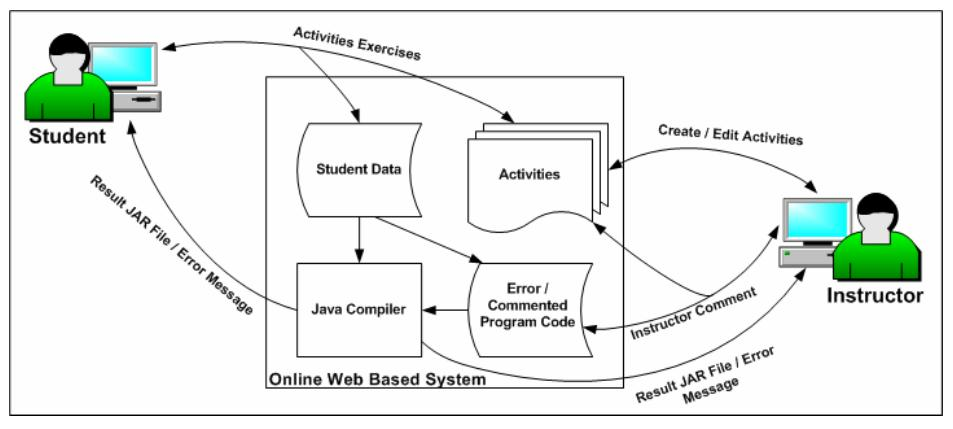
\includegraphics[width=0.9\linewidth, keepaspectratio =
1]{./images/SystemArch02_OUHK_DistanceEdu.jpg}
\caption{Prikaz interakcije med študentom in mentorjem s spletnim
  portalom \cite{ITaLCP_DistanceEdu}.}
  \label{fig:OUHK_workFlow}
\end{figure}

Študent lahko pregleduje vse aktivnosti in si naloži katero koli izmed
njih. Omogočeno ima, da program prevede na strežniku, ko prevajalnik
naleti na napake, strežnik vrne napako na spletno stran. Če študent
naleti na težavo, ki je povezana z reševanjem aktivnosti, lahko pošlje
prošnjo za pomoč svojemu mentorju. Ko se mentor prijavi v sistem, ima
vpogled v napako in na začasno delovno datoteko študenta, mentor lahko
zaganja prevajalnik na tem začasnem projektu študenta. Ko mentor
popravi programsko napako, odgovori študentu in poda komentar na
programsko kodo študenta. Študent ima vpogled v komentarje in
predloge, ki jih je posredoval mentor \cite{ITaLCP_DistanceEdu}.

%%NJihova diskusija, zaključek in nadaljnjo delo.

Na univerzi v US \cite{mentalModels} je okrog strategije kognitivnega
konflikta nastalo spletno okolje, ki naj bi izboljšalo mentalne modele
ključnih programskih konceptov. Učni model je sestavljen iz štirih
korakov:

\begin{itemize}
\item \textbf{Predhodni korak:} mentor razišče, kakšni so predhodni
 mentalni modeli študentov, in identificira neprimerne.
\item \textbf{Korak kognitivnega konflikta:} v študentovi predstavi
  mora sprožiti tak dogodek, ki v študentu izzove neskladje z njegovo
  predhodno predstavo in s tem se študenta potisne v konfliktno
  situacijo.
\item \textbf{Korak konstruiranja modela:} vizualizacija študentu
  pomaga ustvariti pravo mentalno predstavo.
\item \textbf{Korak aplikacije:} študent mora rešiti programsko
  nalogo z na novo ustvarjeno mentalno predstavo.
\end{itemize}

Spletno učno okolje podpira programski jezik \textbf{Java}. Za učenje
programskih konceptov je na spletni strani vsak posamezen koncept povezan s
potjo, ki predstavlja načrt potovanja. Poti konceptov se povezujejo tako, da se
ti nadgrajujejo, saj znanje določenega koncepta potrebuje neko predznanje
prejšnjega. Tako za razumevanje določevanja reference najprej potrebujemo
predznanje o spremenljivkah ali npr. preden se študenti učijo, kako se podajajo
parametri v podprograme, morajo najprej razumeti, kaj je obseg nekega
podprograma. Torej je vrstni red spoznavanja programskih konceptov pomemben. Med
potmi so gumbi, ki predstavljajo vsak koncept. Na vsakem gumbu je označen rdeč
križ, kar pomeni, da študent še ni spoznal koncepta. Ko študent opravi naloge,
povezane s posameznim konceptom, se rdeč križ spremeni v zeleno kljukico. Ko
študent vstopi v koncept, se izpiše študentova zgodovina z nalogami tega
koncepta. Vsaka naloga vsebuje tako vprašanje, ki sproži konfliktno situacijo v
mentalnem modelu študenta. Nato študenti dobijo učni material v vidni obliki. Za
vizualizacijo uporabljajo orodje
\href{https://cs.joensuu.fi/jeliot/}{\textbf{Jeliot}}, ki dinamično upodablja
izvajanje javanskih programov. Za pravilnost razumevanje mentalnega modela mora
študent odgovoriti na dodatna vprašanja. Če študentovi odgovori niso v skladu s
podanim mentalnim modelom, dobi študent povratno informacijo o nepravilnem
odgovoru. Naslednji korak je ta, da mora študent zagnati vizualizacijo dela
programske kode, ki si ga je prej moral predstavljati. Tako ima možnost, da
zazna nepravilnost v svojem mišljenju in tako lahko gradi na pravilnem konceptu
\cite{mentalModels}.

%% QUTA
V preteklosti je bilo razvitih mnogo orodij, ki so nastala ravno zaradi
raziskovanja učenja programiranja, vendar mnoga od teh zahtevajo, da
študenti pišejo celotne programe od začetka do konca. Spletni portal
v primeru QUTA uči programiranja v programskem jeziku Java in ima
 naslednje zmožnosti \cite{thesisAWebP}.

\begin{enumerate}
\tightlist
\item Spletni portal za programiranja, ki omogoča naloge tipa ``zapolni
   prazna mesta''. % pri "zapolni prazna mesta se ti izpiše Ž namesto z!
\item Ogrodje za analizo, ki preverja kakovost in pravilnost, nalog
   tipa "zapolni prazna mesta".
\item  Samodejni sistem za dajanje povratnih informacij, ki sporoča
   prilagojena sporočila prevajalnika in formalni odziv študentom in
   njihovim mentorjem. Poročilo vsebuje kakovost napisanega programa,
   strukturo in pravilnost glede na programsko analizo.
\end{enumerate}

\subsection{Rezultati izvedenih rešitev SPUP}
\label{sec:rezultati_izvedenih_rešitev}

Večina študentov smeri računalništva na OUHK nima predhodnih izkušenj
v programiranju s programskim jezikom \textbf{Java}. Sistem se
uporablja kot spletno okolje za učenje programiranja. Študentom je s
tem dana množica aktivnosti oz. nalog, ki jih morajo sami uspešno
opraviti. To lahko počnejo kadarkoli in kjerkoli. Študentom ni
treba nastavljati programskega okolja, študenti vse programe, ki
jih napišejo, lahko takoj prevedejo in jih zaganjajo na svojih
računalnikih. Uporaba spletnega portala je pokazala, da so študentje
oddali 100 \% programskih nalog, napisanih v Javi. Kar kaže na to, da so
študentje samozavestno reševali naloge in jih oddajali. Pred uporabo
spletnega portala je oddaja nalog bila 80 \%.

Kot pravijo avtorji članka in portala \cite{ITaLCP_DistanceEdu}, je to
šele začetek uporabe spletnega portala, ki nudi osnovno
funkcionalnost. V nadaljevanju nameravajo dodati še inteligentni
sistem, ki bo nadzoroval napredek študentov.

Za izboljšanje mentalnih modelov, ki avtorji predlagajo konstruktivno
naravnan učni model, ki vključuje strategijo kognitivnega konflikta in
vizualizacijo programov. Zgodnje preizkušanje strategije kognitivnega
konflikta pokažejo, da so študenti bolj zavzeti za učni material in jih
motivira tako, da si prej ustvarijo pravilno mentalno predstavo
\cite{mentalModels}.

Tudi začetniki, ki uspešno premagajo začetne ovire in se lotijo
takojšnjega programiranja, imajo zelo slabo napisano in konstruirano
programsko kodo. Pomagati novincem pisati kakovostno programsko kodo
je časovno zelo zahtevno opravilo.

% Torej je pomembno v katerih programskih jezikih se začnemo učiti
% programiranja? Zakaj sta zato primerna? -> Scratch in Python?  Kje
% je določeno na državnem nivoju da se učit ravno ta dva programska
% jezika

Rezultat dela avtorjev spletnega portala QUTA gre še nekoliko naprej
od OUHK in v njihov spletni portal vgradijo odziv spletnega portala,
ki javlja o pravilnosti programa in o kakovosti. Ogrodje
\emph{(ang. framework)} za analizo programske kode vsebuje naslednje
komponente \cite{thesisAWebP}:

\begin{itemize}
\tightlist
\item
  sintaktično ali semantično opozarjanje na napake ali napake
  prevajalnika,
\item
  odziv na kakovost in pravilnost programske kode,
\item
  formalni odziv učitelja oz. komunikacija med učiteljem in učencem.
\end{itemize}

\subsection{Značilnosti SPUP}
\label{sec:značilnosti_spup}

Ena od osnovnih in glavnih komponent pri vseh SPUP je orodje, ki
omogoča pisanje in preizkušanje programske kode. Poimenujemo jo lahko
kot \textbf{spletna aplikacija za programiranje (SAZP)}. Njene
glavne značilnosti so naslednje:

\begin{itemize}
  \item \textbf{urejevalnik besedil}, ki ima lahko osnovne funkcije ali tudi
  zahtevne, ki so značilne za \textbf{IRO};
\item omogočen je zagon napisanega progama z vhodnimi in izhodnimi
  podatki;
\item omogočena je \textbf{povratna informacija}:
  \begin{itemize}
    \tightlist
  \item \textbf{sintaktičnih napak}, ki ju vrne prevajalnik ali tolmač;
  \item \textbf{semantičnih napak}, ki preverjajo želen rezultat napisanega
    programa oz. pravilno rešitev.
  \end{itemize}
\end{itemize}

Iz pregleda SPUP, ki so nastali na univerzah, smo se lahko poučili, kaj
so nekatere značilnosti spletnih portalov. Strnimo te značilnosti, saj
jih bomo pozneje uporabili pri iskanju, kategoriziranju in
vrednotenju. Spletni portal vsebuje naslednje elemente:

\begin{itemize}
\tightlist
\item razdelano vsebino z nalogami oz. aktivnostmi,
\item \textbf{spletno aplikacijo za pisanje programske kode},
\item omogočena je komunikacija med mentorjem in novincem,
\item omogočen je pregled nad napredkom novincev oz. tako imenovan
  \emph{nadzor nad razredom}.
\end{itemize}


%%% Local Variables:
%%% mode: latex
%%% TeX-master: "../diploma"
%%% End:

\newpage
\section{Kriteriji za klasifikacijo spletnih portalov}
\label{sec:kriteriji_za_klasifikacijo_spletnih_portalov}

Spletni portali za učenje programiranja imajo različne značilnosti in
zmožnosti. V poglavju bomo razdelali posamezne kriterije, s katerimi
bomo klasificirali in ovrednotili posamezne spletne portale.

\subsection{Vrsta vsebine}
\label{sec:Razvrstitev_spletnih_portalov}

Po prvem pregledu in iskanju spletnih portalov lahko ugotovimo, da
spletni portali za učenje programiranja ponujajo najrazličnejše vrste
vsebin in njihove kombinacije, kot je na primer, \textbf{tekstovni
  vodič in spletna aplikacija za programiranje}. V posebno kategorijo
bomo uvrstili tudi spletne portale, ki ponujajo \textbf{spletne igre},
ki učijo programiranje. Različne vrste spletnih portalov, ki jih lahko
obravnavamo, so naslednje:

\begin{itemize}
\tightlist
\item \textbf{tekstovni vodiči},
\item \textbf{video vodič},
\item \textbf{spletna aplikacija za programiranje}, kot smo jo
  definirali v poglavju \ref{sec:značilnosti_spup},
\item \textbf{spletne igre},
\item \textbf{kombinacija} vrst vsebin, ki jih lahko še razdelimo na:
  \begin{itemize}
    \tightlist
  \item \textbf{najosnovnejša kombinacija} (\emph{tekstovni vodič + preizkus kode});
  \item \textbf{napredna kombinacija} (\emph{različne vrste vodičev +
      spletna aplikacija za programiranje}), ki tvorijo \textbf{vadnice}.
  \end{itemize}
\end{itemize}

V tej diplomskem delu se ne bomo podrobno ukvarjali s tem, katera izmed vrst
vsebin predstavlja boljše zmožnosti za prenos znanja. Vsaka ima svoje
prednosti in slabosti, zato bomo za vsako izpostavili le bistvene
pozitivne značilnosti in tudi slabosti. Zanimale nas bodo predvsem
tiste \textbf{kombinirane} vrste vsebin, ki bodo predstavljale čim bolj
celovit spletni portal za učenje programiranja, kot smo ga definirali
v poglavju \ref{sec:značilnosti_spup}.

\subsubsection{Tekstovni vodiči}

Spletni vodiči veljajo za starejše metode podajanja znanja na
spletu. Za njih je značilno, da uporabnika vodijo \textbf{po korakih}
do nekega določenega cilja, kako nekaj narediti, ali specifičnega
znanja. Besedilo, ki podaja znanje, je opremljeno s
\textbf{primeri}. \cite{wiki:tutorials}

Značilni predstavnik takih vodičev je spletna stran
\url{https://docs.python.org}, na kateri najdemo vso dokumentacijo
programskega jezika \textbf{Python}. Na strani najdemo tudi vodiča z
naslovom \emph{\href{https://docs.python.org/3/tutorial/index.html}{The
  Python Tutorial}} \cite{web:TPythonTut}.

\begin{figure}[h!]
  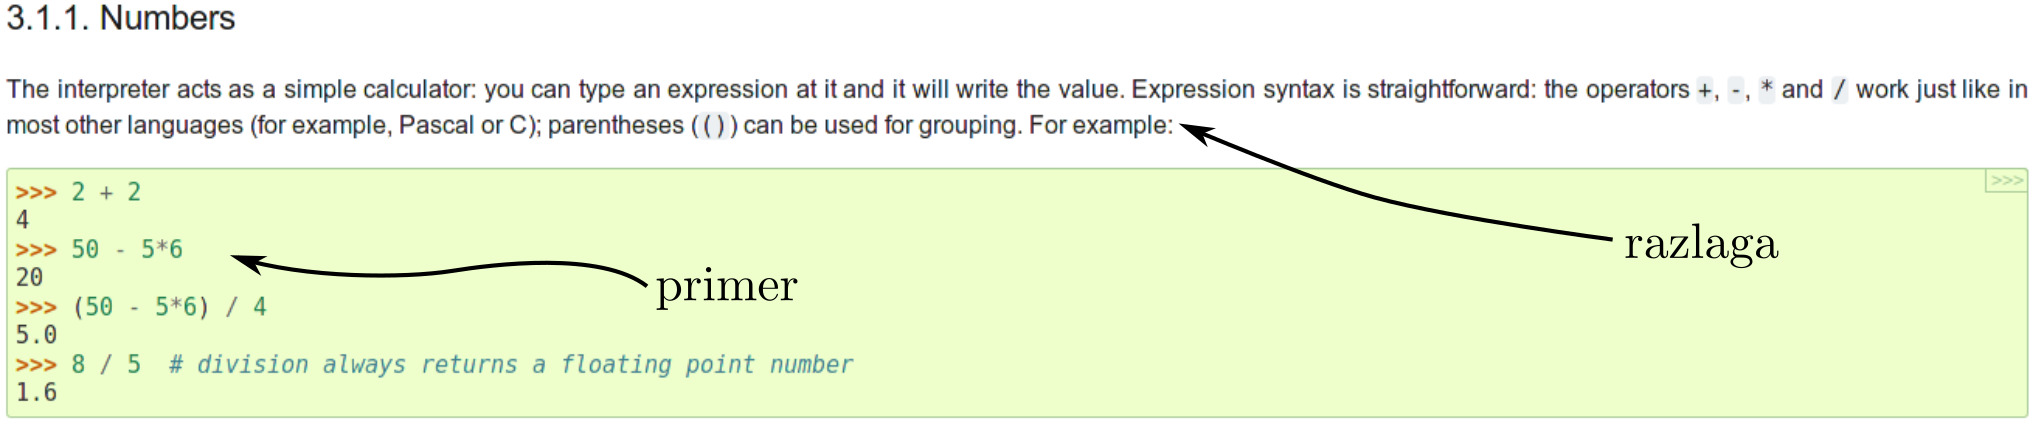
\includegraphics [width=1\linewidth, keepaspectratio =
  1] {./images/sc_web/tPyTut_01.jpg}
    %\def\svgwidth{\columnwidth}
    %\input{./pdf_tex/tPyTut_01.pdf_tex}
      \caption{Zaslonski posnetek poglavja z vodiča
      \emph{\href{https://docs.python.org/3/tutorial/index.html}{The
          Python Tutorial}} s primerom \cite{web:TPythonTut}.}
    \label{fig:scr:web:tPyTut}
\end{figure}

Spletne vodiče pri pouku uporabljamo na podoben način, kot bi vodiča,
napisanega na učnem listu z \textbf{metodo dela s tekstom}. Sicer je
pomembno, da učenci usvojijo uporabo spletnih vodičev, vendar so
spletni vodiči marsikdaj prezahtevni za uporabo, sploh na osnovnošolskem nivoju, z vso tehnično dokumentacijo. Negativna stran spletnih
vodičev je še ta, da ne moramo neposredno s spletne strani preizkušati
primerov programske kode, kar je slabo tudi z motivacijskega vidika.

\subsubsection{Video vodiči}
\label{sec:video_vodici}

Z razmahom video vsebin na spletu so marsikateri spletni vodič
dopolnili oz. jih zamenjali video vodiči. Popularno je postalo
zajemanje oz. \textbf{snemanje lastnega namizja}. Video vodiče najdemo
za številna področja, od uporabe določene programske opreme in vse do
programiranja. Ena izmed prednosti video vodičev je
ta, da ti omogočajo nazornejši prikaz nekega postopka po
korakih. Preden sami opravimo nek postopek, lahko v video posnetku
opazujemo vsak korak, potek miške in poleg tega poslušamo razlago, če
je ta vključena. Številne študije kažejo, da je učenje z multimedijo,
torej kombinacijo zvoka in slike,  učinkovitejše kot samo poslušanje ali
branje teksta \cite{web:multimediaL}. V razredu je uporaba video
vodičev lahko koristna pri samostojnem in domačem delu. Uporaba
video vodičev ima tudi slabe strani, v njih lahko predstavimo dosti
manj vsebine in iskanje po vsebini v video ni preprosto, kot je to pri
tekstu.

Eden izmed spletnih portalov, ki je specializiran za podajanje znanja
z video vodiči, je \emph{\href{https://www.udemy.com}{Udemy}}
\cite{web:udemy}. Na njem lahko vsakdo  postane učitelj in pripravi
učne ure z različnih področij, ne samo z računalniške
znanosti. Nekateri sklopi učnih ur so v celoti brezplačni, kljub temu
je večina plačljivih.

\begin{figure}[h!]
    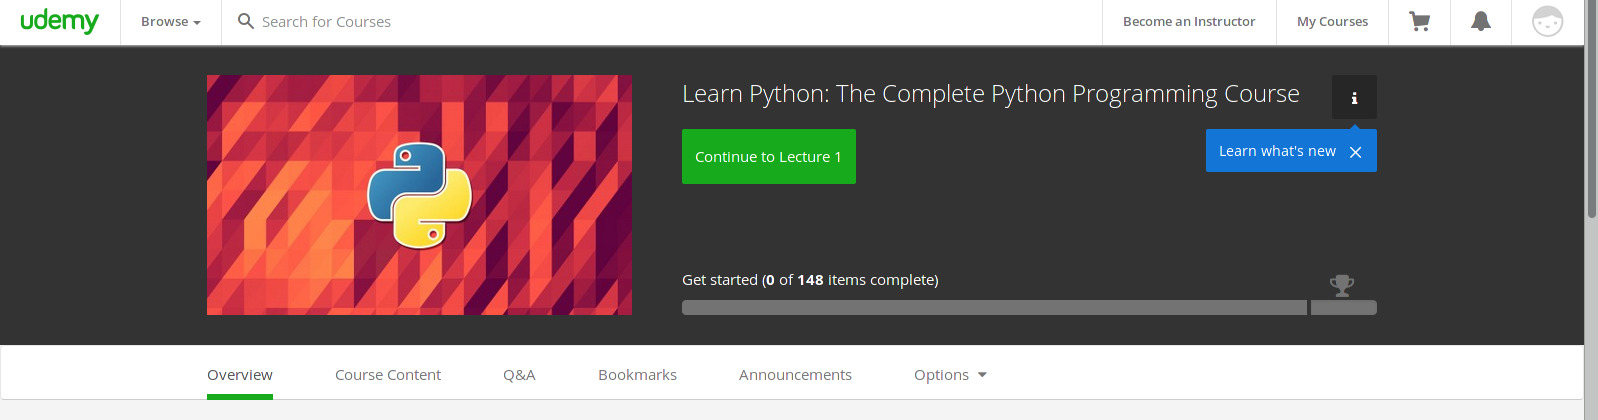
\includegraphics [width=1\linewidth, keepaspectratio =
    1] {./images/sc_web/udemy_01.jpg}
    \caption{Uvodna stran enega izmed video vodičev za učenje Pythona
      \cite{web:udemy}.}
    \label{fig:scr:web:udemy}
\end{figure}

\subsubsection{Spletna aplikacija za programiranje}
\label{sec:spletna_app_programiranje}

Nekatere spletne strani ponujajo le spletno aplikacijo za
programiranje, kot smo jo povzeli v poglavju
\ref{sec:značilnosti_spup}. Taki spletni portali ne ponujajo vsebine,
ponujajo le aplikacijo, ki jo uporabimo kot \textbf{orodje}. Ali pa
ponujajo le toliko vsebine, kot je potrebno, da se uporabnik nauči
uporabljati spletno aplikacijo. Kljub temu da nas zanimajo celoviti
spletni portali, ki ponujajo tudi vsebino, nas bodo podrobneje
zanimala tudi orodja, saj so ta ključna za nekatere prednosti, ki jih
ponujajo spletni portali za učenje programiranja. Predstavnik takega
orodja je \emph{\href{http://pythonfiddle.com/}{Python Fiddle}}
\cite{web:pythonfiddle}. Omogoča osnovni urejevalnik besedila (slika)
z barvanjem programske kode, s predlogami za samodokončanja izpisa
vgrajenih funkcij. Uvozimo lahko datoteke in jih delimo. Zaganjamo
napisane programe, izhodni podatki se izpišejo v konzoli.

\begin{figure}[h!]
    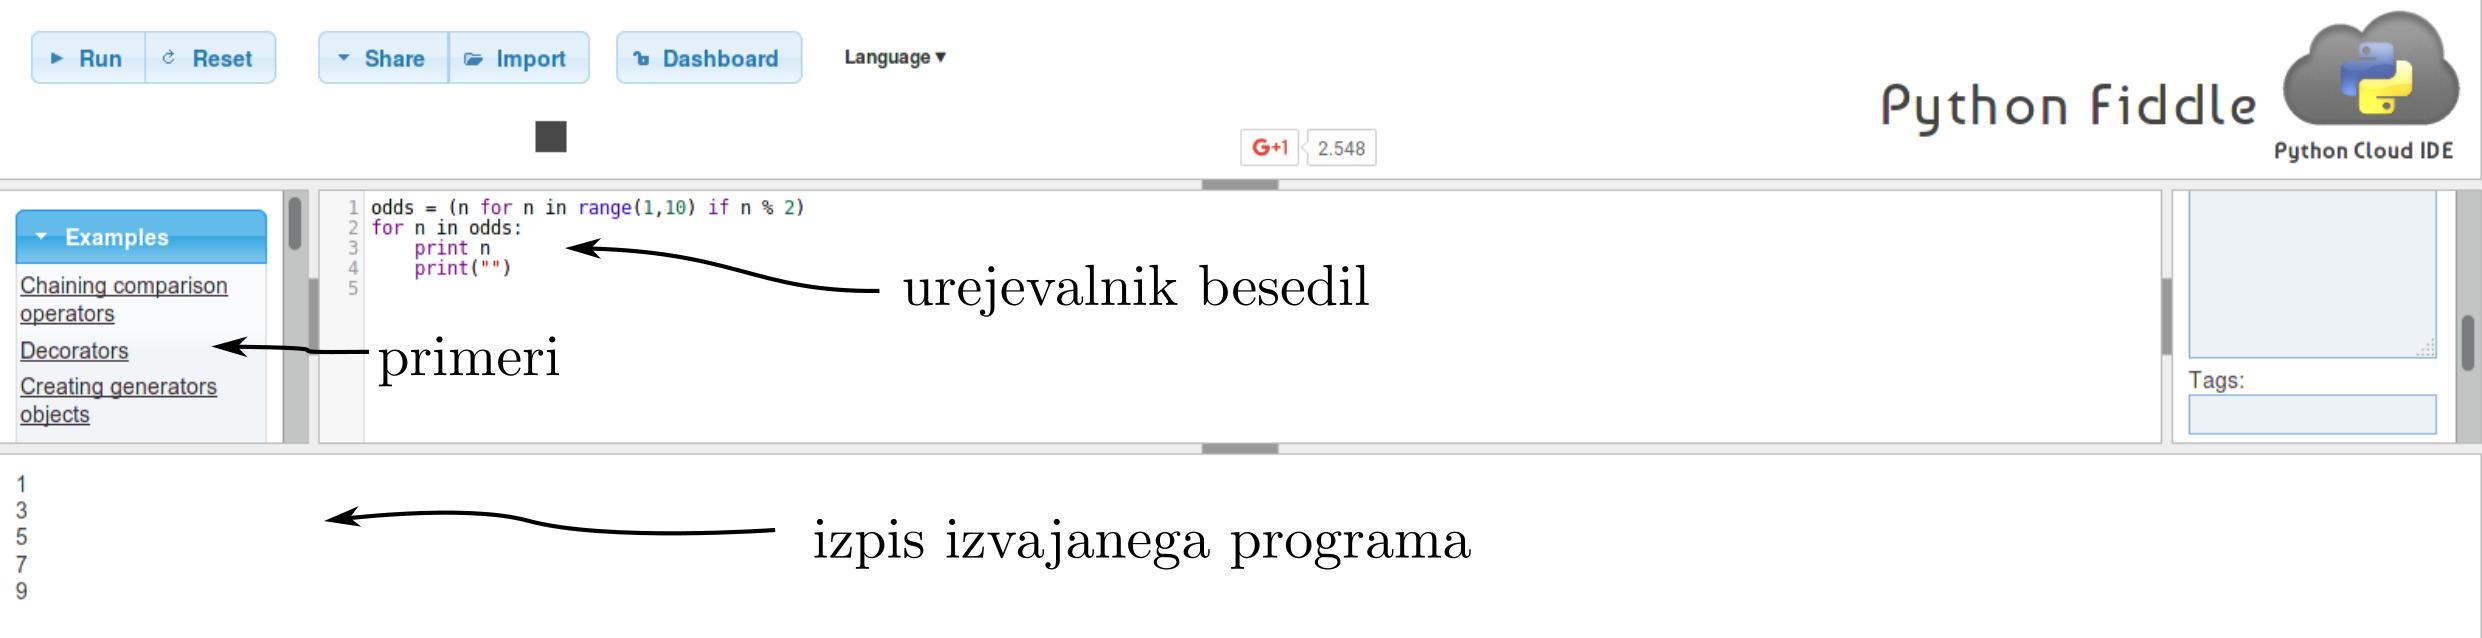
\includegraphics [width=1\linewidth, keepaspectratio =
    1] {./images/sc_web/PythonFiddle_01.jpg}
    \caption{Zaslonska slika spletne aplikacije za programiranje
      \emph{\href{http://pythonfiddle.com/}{Python Foddle}}
      \cite{web:pythonfiddle}.}
    \label{fig:scr:web:PyFiddle}
\end{figure}

Spletne tehnologije so danes zelo napredovale in že nekaj let se
aplikacije in podatki selijo v \textbf{oblak}. Te aplikacije in
podatki so dostopni kjerkoli. V \textbf{oblaku} se razvijajo
številna profesionalna okolja \textbf{IRO}, ki omogočajo delo na
večjih projektih in ponujajo napredne funkcije IRO, ki smo jih drugače
lahko imeli le z namiznimi aplikacijami. Navedimo dva primera:
\emph{\href{https://codenvy.com/}{Codenvy}} \cite{web:codeenvy} in
\emph{\href{https://c9.io/}{Cloud9}}\cite{web:cloud9}. Oba ponujata
profesionalni IRO v oblaku. Za uporabo v šoli sta ti dve okolji preveč
zahtevni in jih ni smiselno uporabljati pri poučevanju novincev. S
tem jim otežimo učenje programiranja, saj potrebujejo čas, da
spoznajo in se naučijo uporabljati IRO.

\subsubsection{Spletne igre}
\label{sec:spletne_igre}

Na spletu obstajajo številni spletni portali, ki učijo in spodbujajo k
učenju programiranja z igram podobnimi vsebinami. Vsebina je
razdeljena na stopnje. Igralci napredujejo iz stopnje v stopnjo in pri
tem nabirajo izkušnje, nove veščine in dosežke. Za igranje igre ne
upravljamo gibanja lika v igri s tipkovnico in miško, temveč pišemo
programsko kodo, ki upravlja njihovo početje. Takšni spletni portali
dajejo zelo dobro motivacijsko osnovo, saj se novinci spoznajo na
osnovne principe igranja iger. Primer spletnega portala je
\emph{\href{http://fightcodegame.com/}{Fightcode}}
\cite{web:fightcode} (slika \ref{fig:fightcode}). Igralci programirajo robota v programskem jeziku
JavaScript. Vsak izmed igralcev lahko izzove drugega igralca v boj med
roboti. Za vsako zmago se igralec pomika navzgor po lestvici
najboljših robotov.

\begin{figure}[h!]
    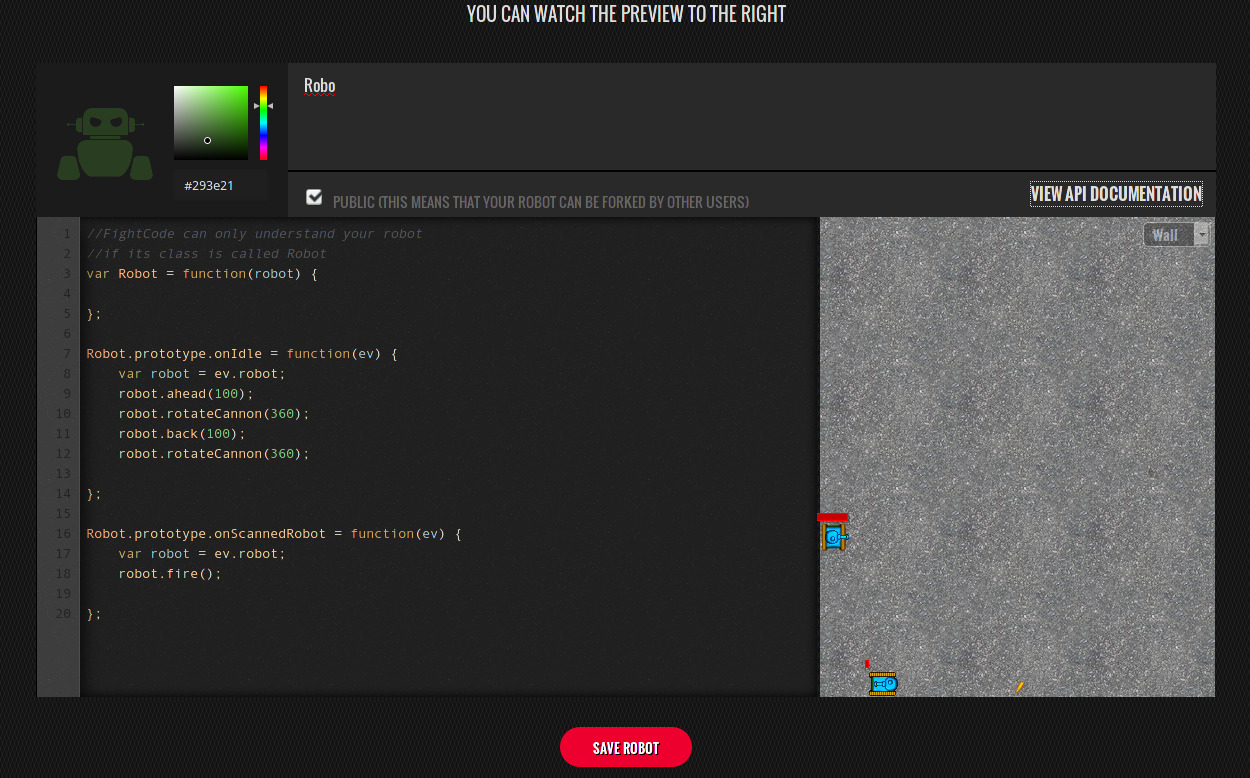
\includegraphics [width=1\linewidth, keepaspectratio =
    1] {./images/sc_web/fightRobot_01.jpg}
    \caption{Zaslonska slika spletne strani
      {\href{http://fightcodegame.com/}{Fightcode}}
      \cite{web:fightcode}.}
    \label{fig:fightcode}
\end{figure}

V nadaljevanju si bomo še podrobneje ogledali značilnosti nekaterih drugih
spletnih iger, ki učijo programirati.

\subsubsection{Kombinirane vrste vsebin}
\label{sec:kombinirane_vrste_vsebin}

V prejšnjih poglavjih smo opisali \textbf{osnovne vrste} spletnih
portalov. Zanimale nas bodo predvsem \textbf{kombinirane vrste}, ki so
sestavljene iz osnovnih. Na spletu najdemo številne kombinacije
spletnih portalov. \textbf{Osnovno kombinirano vsebino} predstavljajo
spletni portali, kot je
\emph{\href{http://www.w3schools.com/}{w3School}} (slika
\ref{fig:scr:web:w3school}) \cite{web:w3school}. Sestavljeni so iz
\textbf{tekstovnih vodičev} in \textbf{najosnovnejšega preizkusa
  programske kode}. Vsak primer v vodiču je opremljen s primerom,
ki ga lahko zaženemo in preizkusimo. Za izvajanje primera
pritisnemo na gumb \textbf{Preizkusi!  (\emph{ang. Try it!})}
Programsko kodo primera lahko tudi spreminjamo in jo ponovno izvajamo.

\begin{figure}[h!]
    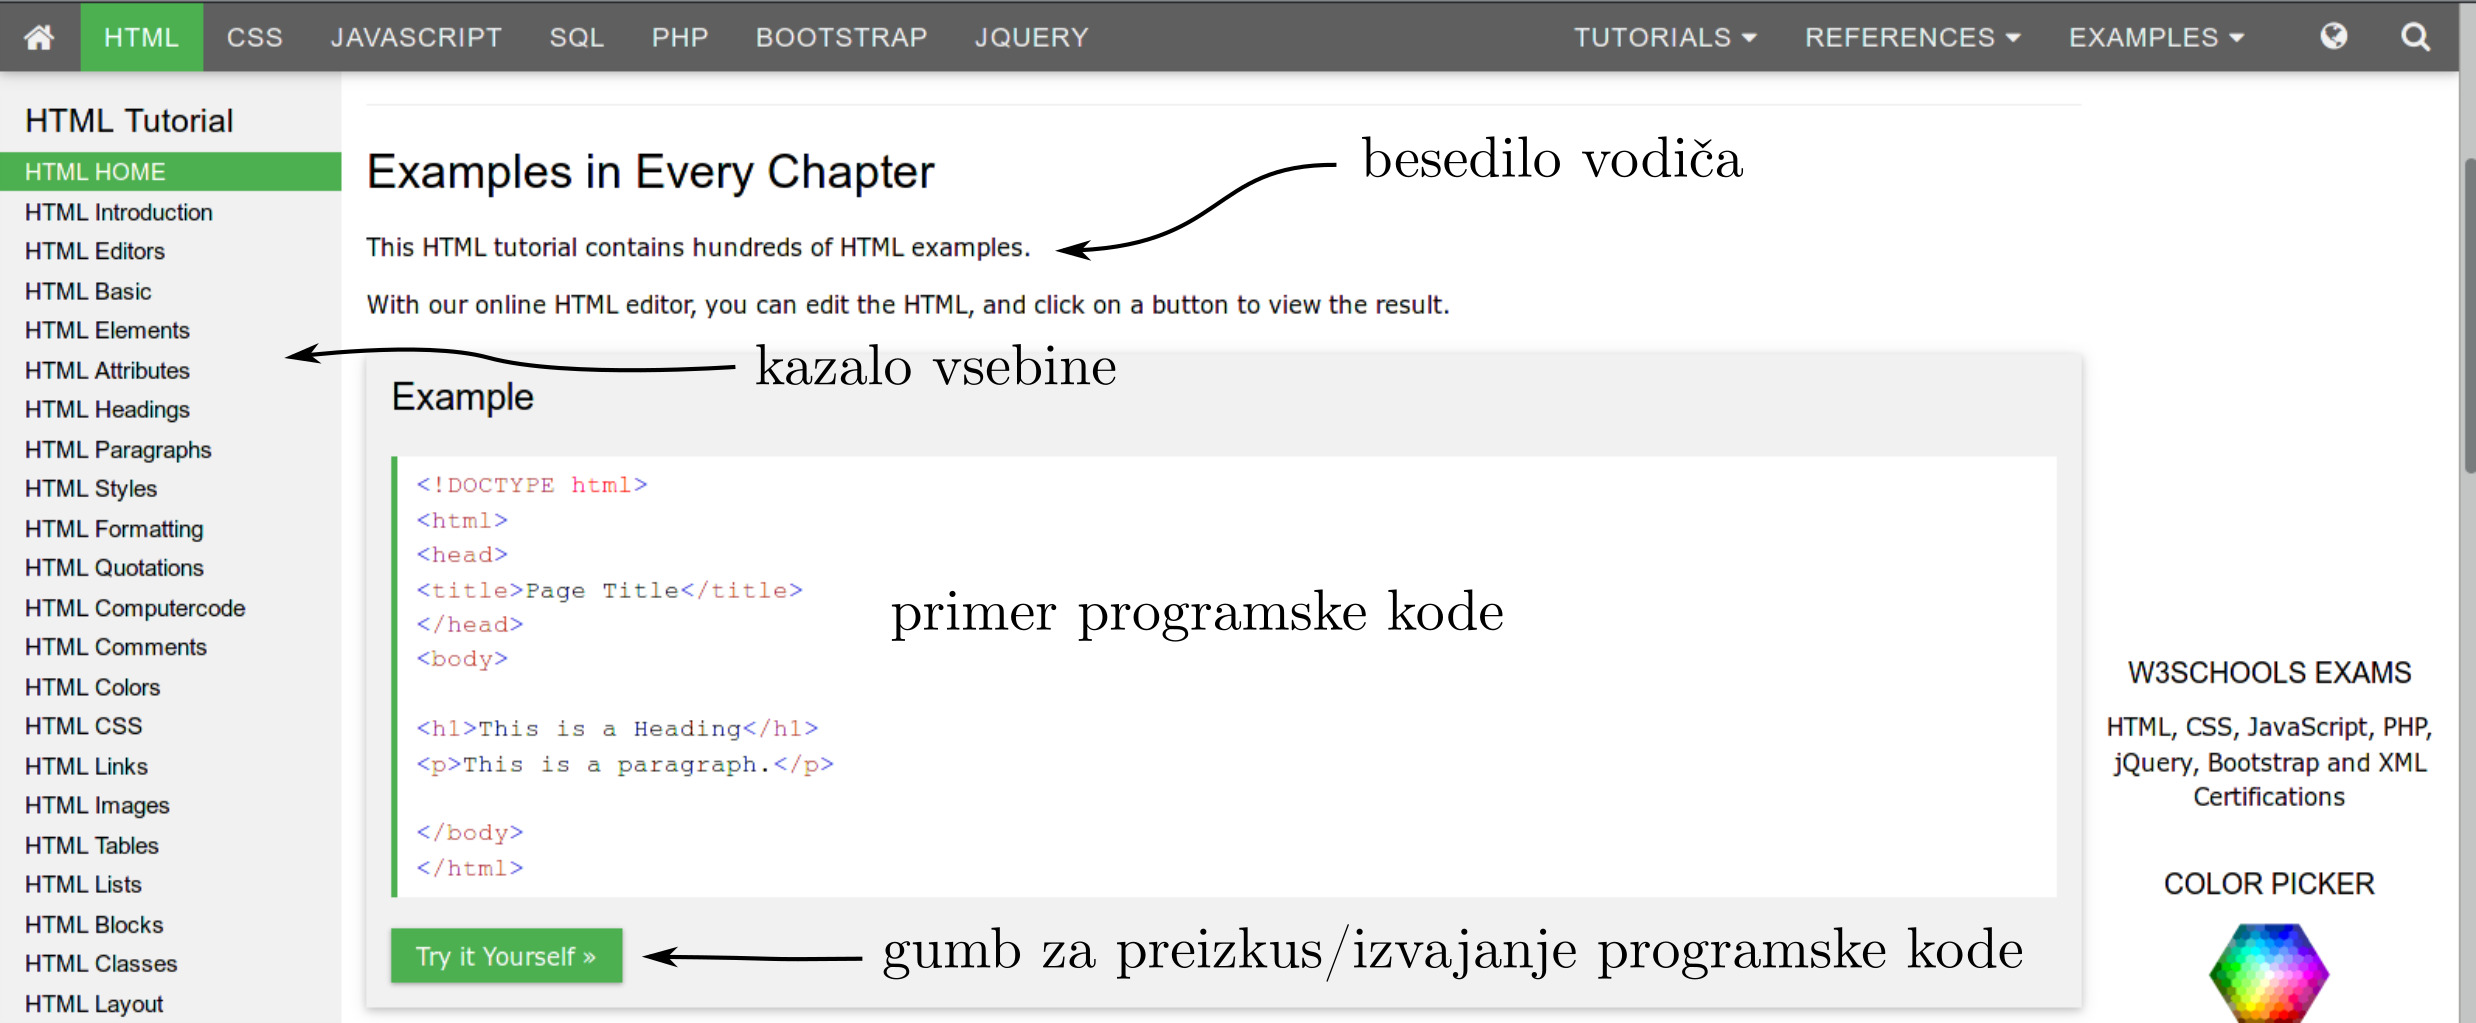
\includegraphics [width=1\linewidth, keepaspectratio =
    1] {./images/sc_web/w3school.jpg}
    \caption{Zaslonska slika spletne strai
      \emph{\href{http://www.w3schools.com/}{w3School}}
      \cite{web:w3school} v poglavju HTML.}
    \label{fig:scr:web:w3school}
\end{figure}

\textbf{Napredno kombinirano vsebino} predstavljajo spletni portali,
ki so sestavljeni iz \textbf{tekstovnega vodiča in/ali video vodičev ter
  spletne aplikacije za programiranje}. Omenimo naslednjega
predstavnika \emph{\href{https://www.codeschool.com/}{Codeschool}}
\cite{web:codeschool}. Taki napredni kombinirani vsebini pravimo \textbf{vadnica}. V njej je navadno podana razlaga, zastavljen
problem oz. naloga, ki ga rešujemo v urejevalniku besedil. V vadnici
imamo navadno še  preverjanje rešitev, torej sintaktično preverjanje
pravilnosti napisane programske kode, ter pravilnost rešitve naloge.

\begin{figure}[h!]
    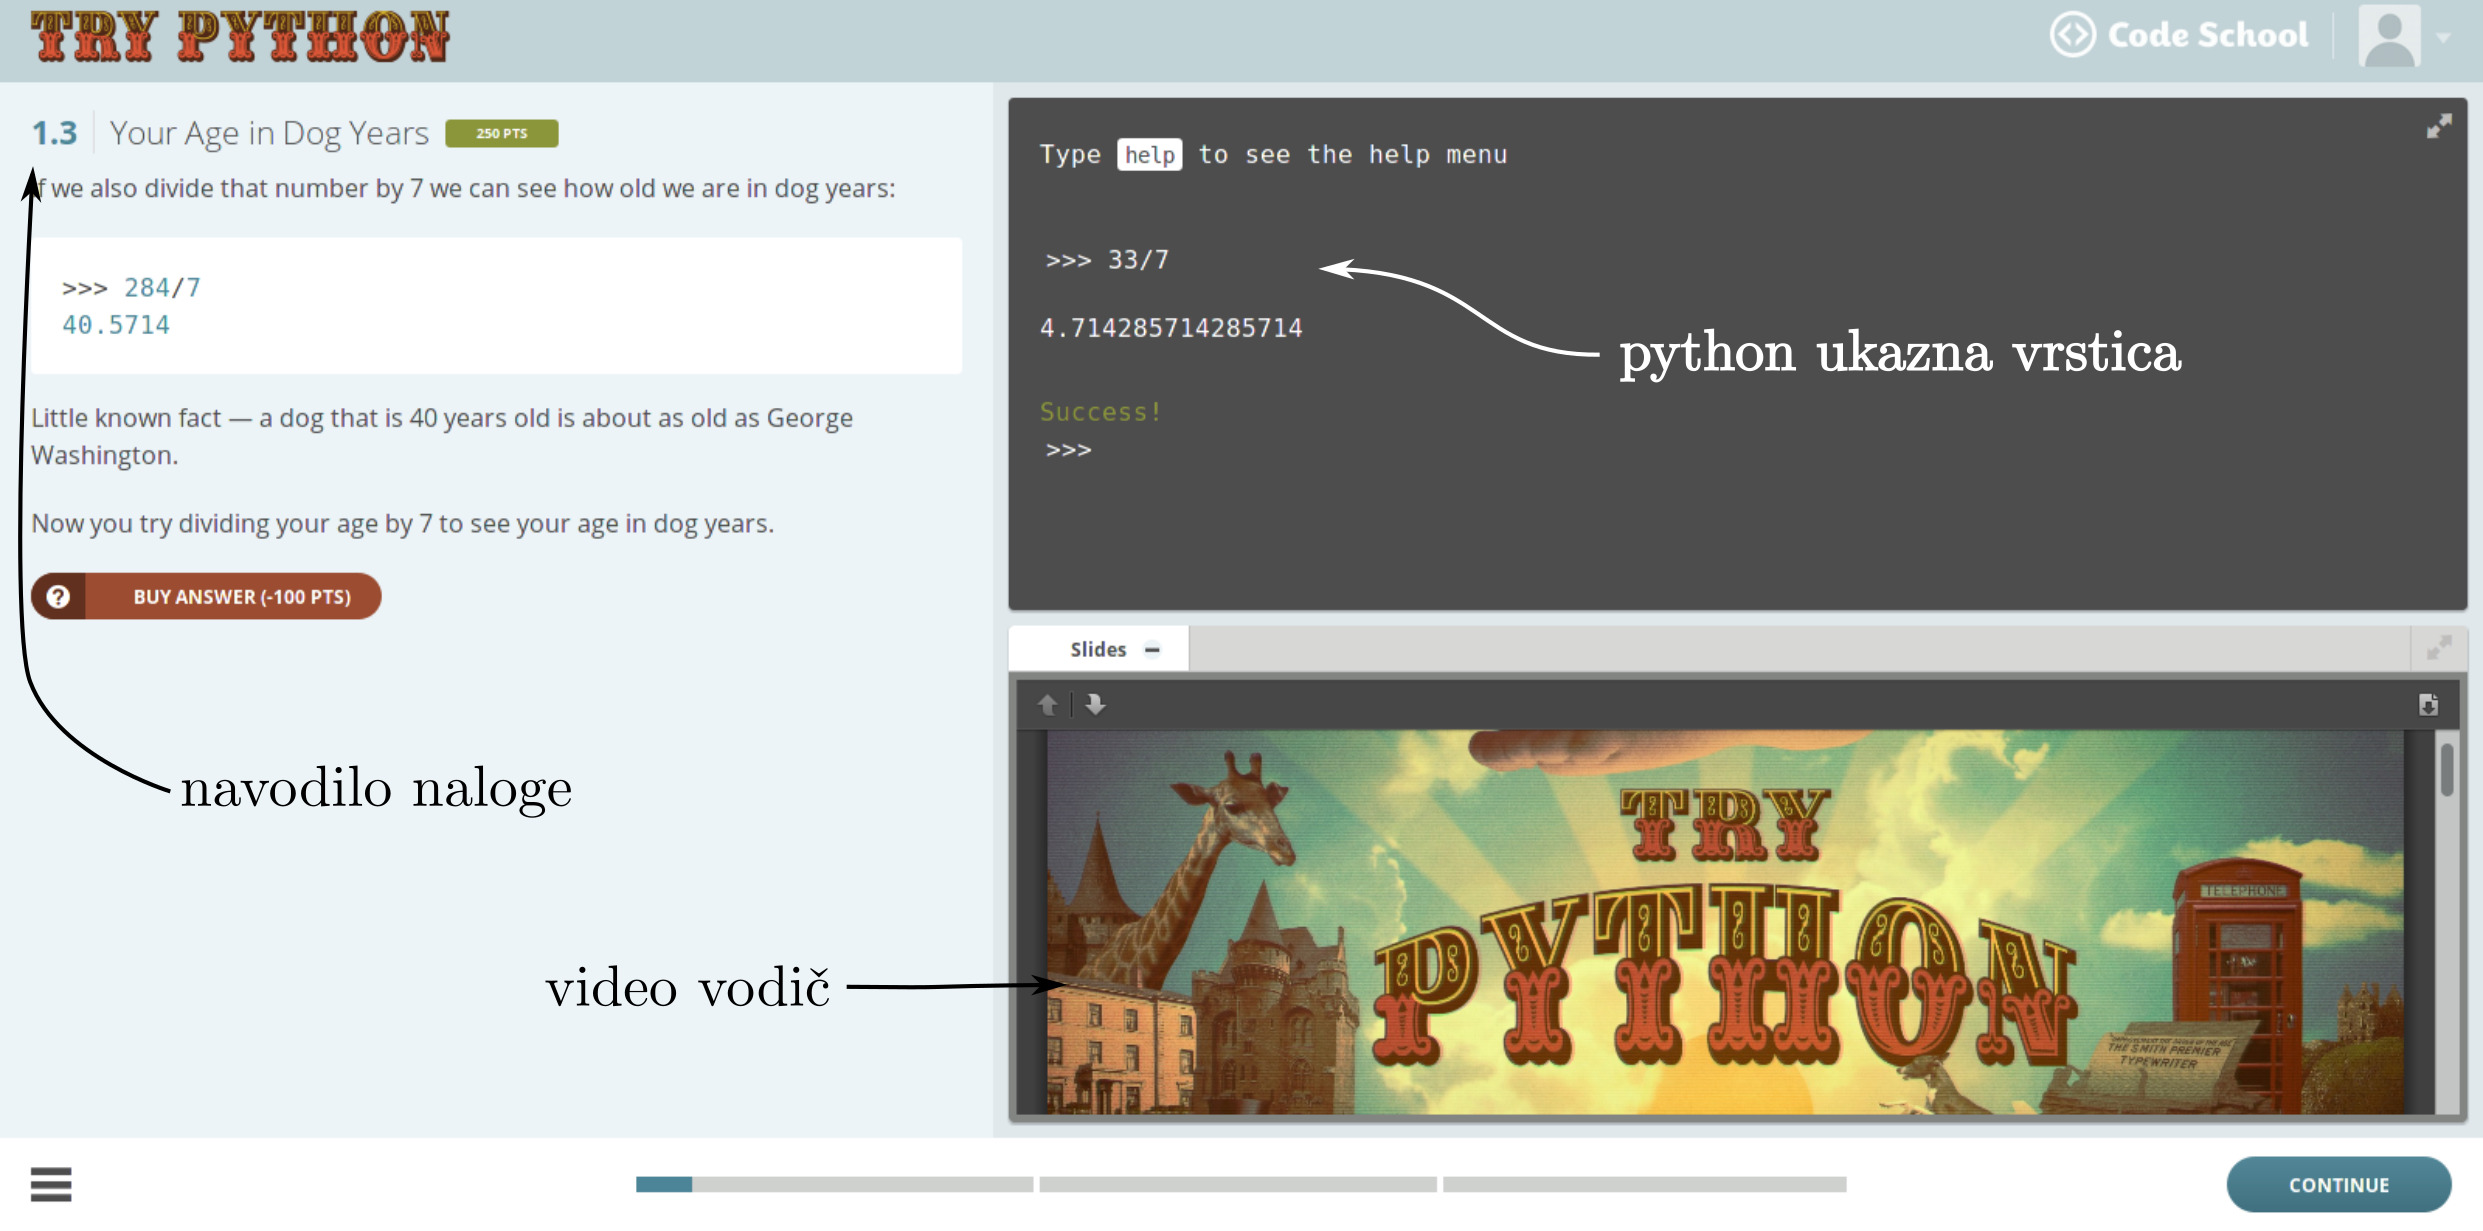
\includegraphics [width=1\linewidth, keepaspectratio =
    1] {./images/sc_web/codeschool_01.jpg}
    \caption{Zaslonska slika spletne strani
      \emph{\href{https://www.codeschool.com/}{Codeschool}}
      \cite{web:codeschool}.}
    \label{fig:scr:web:codeschool}
\end{figure}

Različne kombinirane vsebine imajo različne zmožnosti, ki jih bomo
spoznali na konkretnem primeru v podrobnem pregledu.

\subsection{Jezik spletnega portala}
\label{sec:jezik_spletnega_portala}

Ugotovimo lahko, da večina spletnih portalov uporablja
\textbf{angleščino} kot primarni jezik. Nekateri ponujajo tudi druge
jezike, vendar je \textbf{slovenščina} zaradi majhnosti le malokrat
zajeta, razen v redkih primerih. Angleščina je glavni jezik spleta in
računalniške znanosti, zato je pomembno, da učenci oz. dijaki spoznajo
tudi angleške izraze in jih povežejo s pravilnimi
slovenskimi. Kljub temu da je učenje v slovenskem jeziku predpisano,
lahko vsako učno uro z uporabo spletnih portalov za učenje
programiranja medpredmetno povežemo z angleščino. Zanimalo nas bo,
kateri jezik uporabljajo spletni portali: \textbf{angleščina (da/ne),
  slovenščina (da/ne), drugi (da/ne)}.

\subsection{Ponujena znanja}
\label{sec:vsebina_problemsk_pristop}

Spletne strani za učenje programiranja navadno ponujajo znanja oz.
veščine programiranja z določenim programskim jezikom. Nekatera svojo
ponudbo širijo tako, da ponujajo številne druge projekte, ki
združujejo prej naučeno znanje. Na primer izdelava
\textbf{interaktivne spletne strani}. Za posamezen spletni portal nas
bo zanimalo, ali ponuja samo:

\begin{itemize}
  \tightlist
\item \textbf{znanja/veščine programiranja} oz. učenje določenega
  programskega jezika,
\item \textbf{znanje algoritmov} ali tudi
\item \textbf{druga projektna znanja/veščine} (npr. izdelava spletne
  strani).
\end{itemize}

% Zanimajo nas osnovna načela. -> Razdelaj na načela

\subsection{Programski jeziki}
\label{sec:_zanaja_programski_jeziki}

Zanimalo nas bo, katere programske jezike ponuja nek spletni
portal. Najpogostejše programske jezike smo opisali v poglavju
\ref{sec:programski_jeziki}, v prvi vrsti nas bodo zanimali spletni
portali, ki ponujajo najpopularnejše programske jezike in tiste, ki
se v izobraževanju uporabljajo pri nas. Prednost bodo imeli tisti,
ki ponujajo Python. Večina takšnih spletnih portalov ponuja več
programskih jezikov.

\subsection{Težavnostna stopnja}
\label{sec:težavnostna_stopnja}

Vsak spletni portal je namenjen svojemu občinstvu, zato se razlikujejo tudi po
težavnostni stopnji, čeprav govorimo o novincih. Glavna težavnostna razdelitev
bo na \textbf{osnovo} in \textbf{srednjo šolo}. Po potrebi bomo podrobneje
razdelili že osnovno šolo, ki je razdeljena na triletja. Večina spletnih
portalov izhaja iz Združenih držav Amerike, zato smo povzeli njihove stopnje
šolanja (\ref{tab:primerjava_šolski}), saj nekatere strani uporabljajo
\textbf{K-12} formulacijo za definicijo težavnosti oz. prilagoditev učnemu
načrtu. V podrobnem pregledu bomo ocenili, kateri težavnostni stopnji ustreza
spletni portal.

\begin{table}[!h]
\caption{Primerjava starosti in stopnje šolanja šolskega sistema v ZDA
  in Sloveniji \cite{wiki:k12}.}
\label{tab:primerjava_šolski}
\begin{tabular}{
  | p{0.33\linewidth-2\tabcolsep} |
  p{0.33\linewidth-2\tabcolsep} |
  p{0.33\linewidth-2\tabcolsep} |  }
\hline
  \rowcolor{sbase01!100}
  \textbf{Leta} & \textbf{ZDA K-12 naziv} & \textbf{SI Primerjava} \\
        \hline
      6-10    & \emph{Elementary school} & \textbf{1. in 2. triletje
                                             OŠ}\\
        \hline
      10-14    & \emph{Middle school} & \textbf{3. triletje OŠ} \\
        \hline
  10-14    & \emph{High school} & \textbf{Srednja šola} \\
  \hline
\end{tabular}
\end{table}

%Razdelaj načele problemski pristop. postopnosti in sistematičnosti.
\subsection{Upoštevanje učnih načel}
\label{sec:upoštevanje_načel}

Za uspešno delo in uporabo SPUP v razredu je dobro, da vsebine, ki jih
najdemo na spletu, sledijo že v samem jedru nekaterim \textbf{načelom}, ki jih
upoštevamo tudi drugače pri pouku.

\begin{description}
\item[Problemski pristop (Da/Ne)], zanima nas ali spletni portali, ki
  ponujajo vsebino, uporabljajo problemsko zasnovane naloge, torej imajo
  v začetku obravnavanja snovi podano oz. predstavljeno, kateri problem
  bomo znali na koncu neke vadnice rešiti. Čeprav je vsebina
  računalniške znanosti in programiranja že po naravi problemsko
  zasnovana, marsikdaj ni najbolje predstavljeno, za kaj je neka stvar
  dobra.
\item[Načelo sistematičnosti (Da/Ne)], lahko potrdimo za tiste
  spletne portale, kjer so posamezni vsebinski sklopi povezani v nekem
  logičnem zaporedju. Kot smo že ugotovili pri pregledu spletnih
  portalov na univerzah, je pomembno, da novinci spoznajo nekatere
  koncepte prej kot druge. Tiste spletne portale, ki bodo imeli neko
  rdečo nit v povezavi vsebine, bomo potrdili kot take.
\item[Načelo postopnosti (Da/Ne)], pripišemo lahko spletnemu portalu,
  ki podaja snov v posameznem vsebinskem sklopu tako, da bo razlago
  in program nadgrajeval postopoma in se težavnost stopnjuje.
\end{description}

\subsection{Uporaba ocenjevanja dosežkov, značilnih za igre}
\label{sec:uporaba_dosežkov}

%ToDo: Slovenski izraz za Gamification.
V izobraževanju se uveljavlja trend ocenjevanja napredka in dosežkov,
ki je tipičen za video igre. To metodo ocenjevanje so poimenovali
\emph{ang. Gamification}. Vsako snov ali nalogo, ki je v osnovi toga,
popestrimo z načinom ocenjevanja tako, da vsako nalogo predstavimo z
različnimi izzivi. Vsaki nalogi oz. izzivu sledijo različne nagrade,
ki jih učenci zbirajo in jim pravimo dosežki \cite{web:edublogger}.

Dosežki v video igrah so prisotni že vrsto let. Dosežki se razlikujejo
po kompleksnosti, vse od zmagoslavne glasbe ob končani stopnji ali
igri pa vse do kompleksnega sistema dosežkov z zbiranjem
značk. Značko igralec dobi, ko na primer zbere dovolj predmetov ali
razišče določen odstotek ozemlja. Poznamo več načinov nagrajevanja
dosežkov. Kot smo že omenili, lahko dosežke predstavimo kot
\textbf{značke} ali za posamezne izzive pripravimo sistem točkovanja. Z zbranih točk se lahko sestavijo \textbf{lestvice
  ali uvrstitve}. V razredu  morajo biti slednje skrbno načrtovane, da
ne pride do prevelikih razlik med učenci, kjer bi se eni lahko
počutili nadrejeni in drugi podrejeni.

Zanimalo nas bo, ali spletne portali, ki učijo programiranja,
uporabljajo kakršen koli sistem ocenjevanja dosežkov, saj za tiste, ki
ga uporabljajo, lahko rečemo, da imajo dodaten motivacijski
faktor. Zapisali bomo \textbf{uporabo dosežkov (da/ne)} in tipe
\textbf{značke, lestvice, zbiranje točk za izkušnje, napredovanja  \dots}

\subsection{Dodajanje lastnih vsebin}
\label{sec:dodajanje_vsebin}

Nekateri spletni portali omogočajo, da pripravimo lastne vsebine, ki
jih potem delimo. Navadno je \textbf{spletna aplikacija za
  programiranje} ali \textbf{vadnica} razširjena tako, da omogoča
sestavljanje programskih nalog. Večina teh je taka, da pripravimo
\textbf{spremno besedilo, začetni program ali ogrodje programa, končno
  različico in pomoč ali namig}. Lahko so dodani tudi \textbf{testni
  vhodni in izhodni podatki}. S podatki, ki smo jih vnesli, imamo
avtomatizirano nalogo, ki jo lahko posredujemo oz. delimo z
novincem. Zanimalo nas bo, ali kateri spletni portal omogoča to
zmožnost, torej \textbf{dodajanje lastnih vsebin (da/ne)}.

\subsection{Upravljanje razreda}
\label{sec:upravljanje_razreda}

Zmožnost upravljanja razreda je velika prednost in olajša administrativno delo
 razreda za mentorja. Osnovni način delovanja je
naslednji. Mentor ustvari razred ali predmet podobno, kot je to možno
pri sistemih spletnih učilnic, kot je
\emph{\href{https://moodle.org/}{moodle}} \cite{web:moodle_site}, in v
učilnico povabi učence. Učitelj s spletne učilnice \textbf{spremlja
  napredek} in \textbf{dosežke posameznega učenca}. Pri nekaterih
portalih je \textbf{omogočena komunikacija} med mentorjem in
novincem. Spletni portali spremljanje učencev navadno ponujajo kot
plačljivo storitve za šole, kar navadno ni najbolj poceni. Zanimalo
nas bo, ali spletni portal ponuja \textbf{upravljanje razreda (da/ne)}
in ali je ta storitev \textbf{plačljiva ali brezplačna}.

\subsection{Dostop do gradiv}
\label{sec:dostop_do_gradiv}

Veliko vsebin na spletu je brezplačnih in jih pri pouku lahko
uporabimo. Mnogo vsebin je tudi plačljivih. Spletni portali, ki imajo
plačljive vsebine, uporabljajo navadno model \textbf{plačevanja
  naročnine} za dostop do vsebin. Uporabnik mora na \textbf{letni ali
  mesečni} ravni odšteti različne zneske. Nekateri izmed portalov, kot
je \emph{Codeacademy}, imajo plačljive le nekatere zahtevnejše vsebine
in storitve. Drugi portali imajo vso vsebino
plačljivo. Obstaja tudi vrsta portalov, kot je \emph{Udemy}, kjer je
potrebno plačati za posamezen učni sklop ali temo.  Plačljivost
dostopa do gradiv lahko razvrstimo na naslednji način, tako da je
dostop:

\begin{itemize}
  \tightlist
\item brezplačen,
\item polplačljiv \emph{(nekatere so brezplačne, druge plačljive)},
\item popolnoma plačljive vsebine.
\end{itemize}

%%Dodaj nekaj (3) spletnih portalov, ki so popolnoma plačljivi!

%%% Local Variables:
%%% mode: latex
%%% TeX-master: "../diploma"
%%% End:

\newpage
\section{Pregled spletnih portalov}
\label{sec:pregled_spletnih_port}

V prejšnjem poglavju smo nastavili kriterije, po katerih bomo lažje
vrednotili spletne portale. Preden se lotimo tega opravila, določimo
še omejitve, katere spletne portale bomo dali v ožji izbor in jih
pregledali. Te določitve bodo nastavili v mislih uporabe pri pouku v
srednji in osnovni šoli. Omejitve za izbor spletnega portala so
naslednje:

\begin{itemize}
  \tightlist
\item spletni portal vsebuje \textbf{spletno aplikacijo za
    programiranje}, katero lahko nastopa tudi samostojno brez vsebine
  in jo uporabljamo kot \textbf{orodje},
\item \textbf{vrsta vsebine} naj bo sestavljena z osnovnih vrst
  oz. naj bo \textbf{kombinirana} vrsta vsebine, ki je lahko
  \textbf{osnovna ali napredna} kombiniranih vsebin oz. vsebuje
  \textbf{vadnice},
\item spletni portal ima dosegljivo vsebino \textbf{brezplačno ali pol
  plačljivo}. 
\end{itemize}

\subsection{Code.org}
\label{sec:Code.org}

V predstavitvi spletne strani je predstavljena statistika, ki je
povzeta iz raziskave v ZDA. Z nje je razvidno, da bo v prihodnje
primanjkovalo kadra za računalniško in informacijsko tehnologijo ter
da premalo šol poučuje računalniško znanost
\cite{web:code.org:promote}. Na
\emph{\href{https://code.org}{code.org}} \cite{web:code.org} pravijo,
da so neprofitna organizacija, ki se je posvetila širjenju dostopa do
poučevanja računalniške znanosti, s poudarkom, ki temelji na ne rasni
diskriminaciji in povečanju ženskega spola pri učenju računalništva
\cite{web:code.org:about}.

Spletni portal je v osnovni sestavljen iz štirih glavnih pod vsebina
(slika \ref{fig:scr:web:code:main}), ena je namenjen
\textbf{študentom}, druga \textbf{učiteljem} in tretja \textbf{Uri
  kode}. Četrti vsebinski sklop je namenjen \textbf{promociji drugih
  spletnih portalov, aplikacijam in strojni opremi}, ki pripomorejo k
učenju računalniške znanosti in programiranja ter so del projekta
\textbf{Ura kode}. Najprej si bomo ogledali slednjega.

\begin{figure}[h!]
    
\includegraphics [width=1\linewidth, keepaspectratio =
    1] {./images/sc_web/code_main_part-v01.jpg}
    \caption{Zaslonska slika dela začetne spletne strani
      \emph{\href{https://www.code.org}{code.org}}
      \cite{web:code.org}, iz katerega je razvidna razdeljenost
      vsebin.}
    \label{fig:scr:web:code:main}
\end{figure}

\subsubsection{Ura kode (\emph{ang. Hour of code})}
\label{sec:ura-kode-ang}

\textbf{Ura kode} so krajši projekti, ki jih lahko organizacije kot so
šole izvedejo v času ene do dveh ur. Celoten projekt je namenjen
promociji računalniške znanosti in programiranju. Vsebine, ki so v
okviru tega projekta so navadno uvodne vsebine.

Povezava na portalu \textbf{Ura kode}
\emph{\href{https://code.org}{code.org}} nas vodi do zbirke vadnic, ki
so del spletnega portala \textbf{code}, prav tako najdemo povezave do
številnih drugih spletnih portalov in vsebin, ki so vključile v
projekt, nekatere smo opisali tudi v nadaljevanju.  Vadnice, ki so
del portala, ponujajo številne začetne vsebine, ki so grajene na neki
znani temi iz sveta računalniških iger ali animiranih filmov.

Primer vadnice, ki smo si jo izbrali je tematsko povzeta s znane video
igre \textbf{Minecraft}. V uvodu vsake vadnice najprej sledi video
uvod znane osebe, v tem primeru je to glavni razvijalec omenjene
igre. V tem uvodnem delu zvemo, zakaj je on postal programer in kaj
bomo počeli v tej uri ter kaj se bomo naučili. V predstavitvi je
predstavljen tudi uporabniški vmesnik vadnice. Uvodni del predstavitve
lahko gledamo kot video ali izberemo zapisan povzetek
predstavitve. Snov, ki je razložena v vadnici je \textbf{uporaba
  ukazov, zank in vejitev}. Vadnica je sestavljena iz več enot. Med
uvedbo nove snovi sledi spet video predstavitev ali različica v
besedilu.

Vadnice so sestavljene z aplikacijo za programiranje \textbf{Code
  studio} (slika \ref{fig:scr:web:codestudio}). Pisanje programske
kode v njej je omogočeno z \textbf{zlaganje gradnikov} ali načinom
\emph{ang. Blockly}, kjer z metodo \textbf{vleči in spusti}
sestavljamo oz zlepljamo, programsko kodo. Podoben programski jezik je
tudi \textbf{Scratch}, ki smo ga opisali v poglavju
\ref{sec:scratch}.

\begin{figure}[h!]
  \centering
    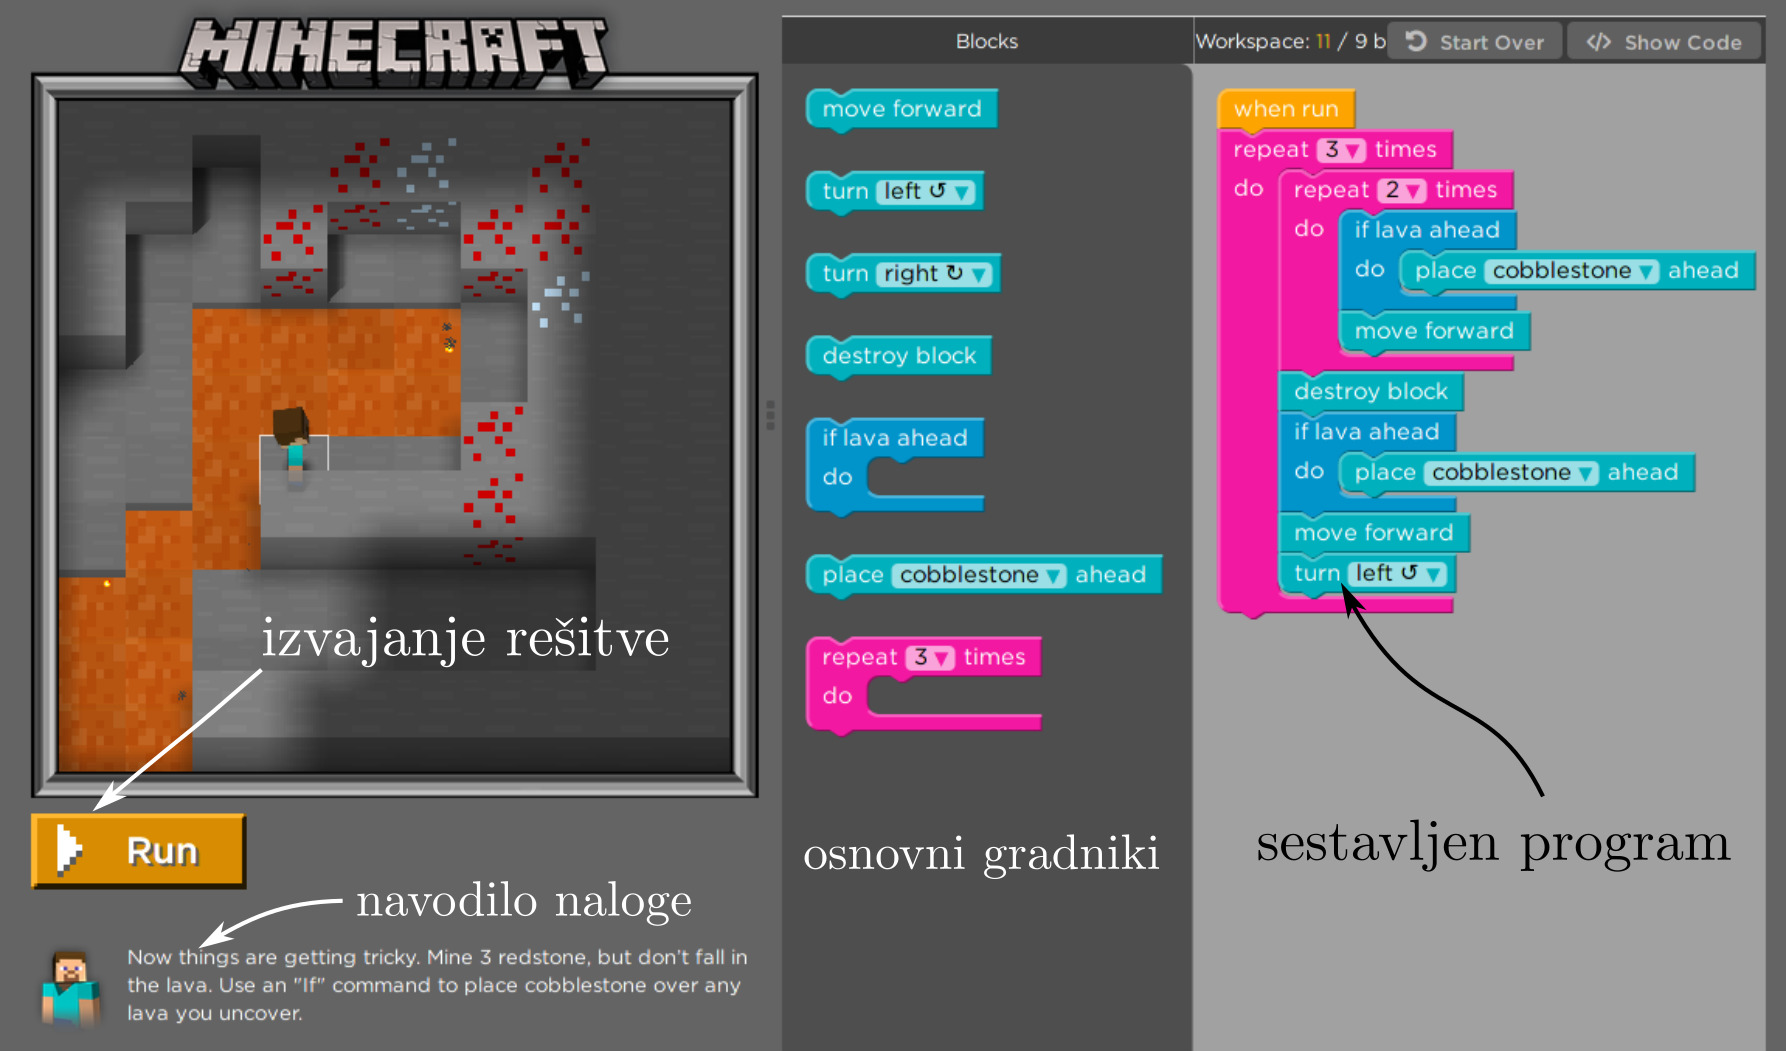
\includegraphics [width=0.65\linewidth, keepaspectratio =
    1] {./images/sc_web/code_cstudiov01.jpg}
    \caption{Spletna aplikacija Code studio v kateri so zgrajene
      vadnice \cite{web:code.org}.}
    \label{fig:scr:web:codestudio}
\end{figure}

Pod temi zlepljenimi gradniki, se ustvarja programska koda v jeziku
\textbf{JavaScript}. Posamezne enote gradijo na znanju sistematično in
postopoma z večanjem težavnostne stopnje. V Vadnicah so omogočeni samo
tisi gradniki, ki jih potrebujemo za rešitev naloge. Večino vsebinskih
sklopov je narejeno tako, da v zadnji vadnici vsebinskega sklopa lahko
prosto uporabljamo vse gradniki, ki smo se jih naučili uporabljati ter
nam ni več potrebno izpolniti konkretnega cilja naloge, da jo
opravimo.

\subsubsection{Code studio}
\label{sec:code-studio}

\textbf{Code studio} ni samo spletna aplikacija, ki omogoča vadnice in
pisanje programske kode temveč je pod stran na kateri novinci najdejo
zbrane vsebine sklope (slika \ref{fig:scr:web:codestudio:main}), ki so
razdeljeni po težavnosti, kateri se spreminja spodnja meja starosti,
zgornja ostaja ista pri 18 letih. Posebna značilnost spletne strani je
tudi ta, da ponuja računalniške vsebine, pri katerih ne potrebujemo
računalnika, tako imenovano \textbf{računalništvo brez računalnika}
ali \textbf{izključene vsebine} (\emph{ang. Unplugged lessons}). Te
vsebine so navadno predstavljene s predstavitvenimi videi in gradivi,
ki jih lahko natisnemo. 

\begin{figure}[h!]
  \centering
  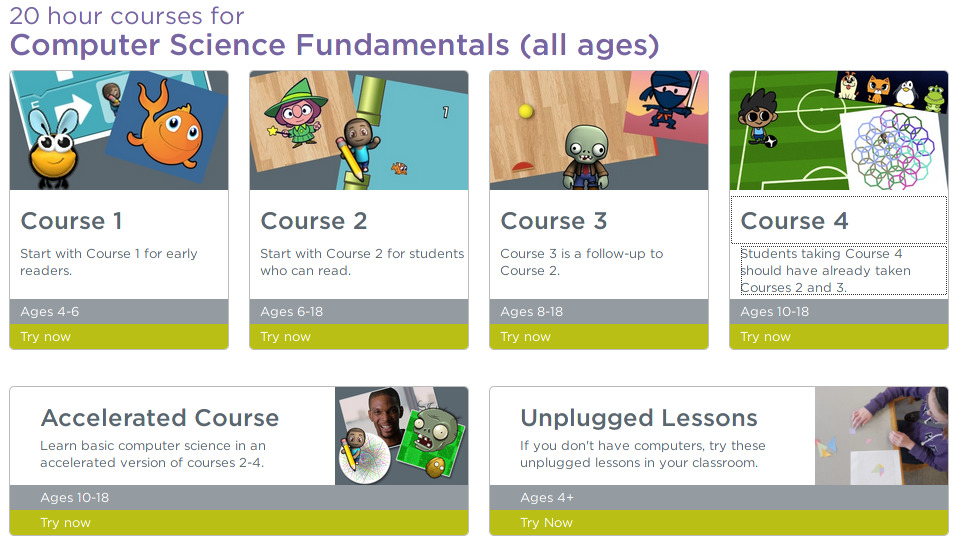
\includegraphics [width=0.65\linewidth, keepaspectratio =
  1] {./images/sc_web/code_cs_main_v01.jpg}
  \caption{Pod stran Code studio za katere lahko nadaljujemo na
    različne vsebinske sklope \cite{web:code.org:studio}.}
  \label{fig:scr:web:codestudio:main}
\end{figure}

Z klikom na posamezni vsebinski sklop, preidemo na stran s
povzetkom. Na tej strani sledimo tudi lastnemu napredku. Vsebine so
razdeljene na manjše tematske sklope, ki so spet sestavljeni iz
posameznih enot oz. vadnic (slika
\ref{fig:scr:web:codestudio:course}). Med posameznimi tematskimi
sklopi najdemo tudi \textbf{izključene vaje}, ki jih predelujemo brez
računalnika.

\begin{figure}[h!]
  \centering
  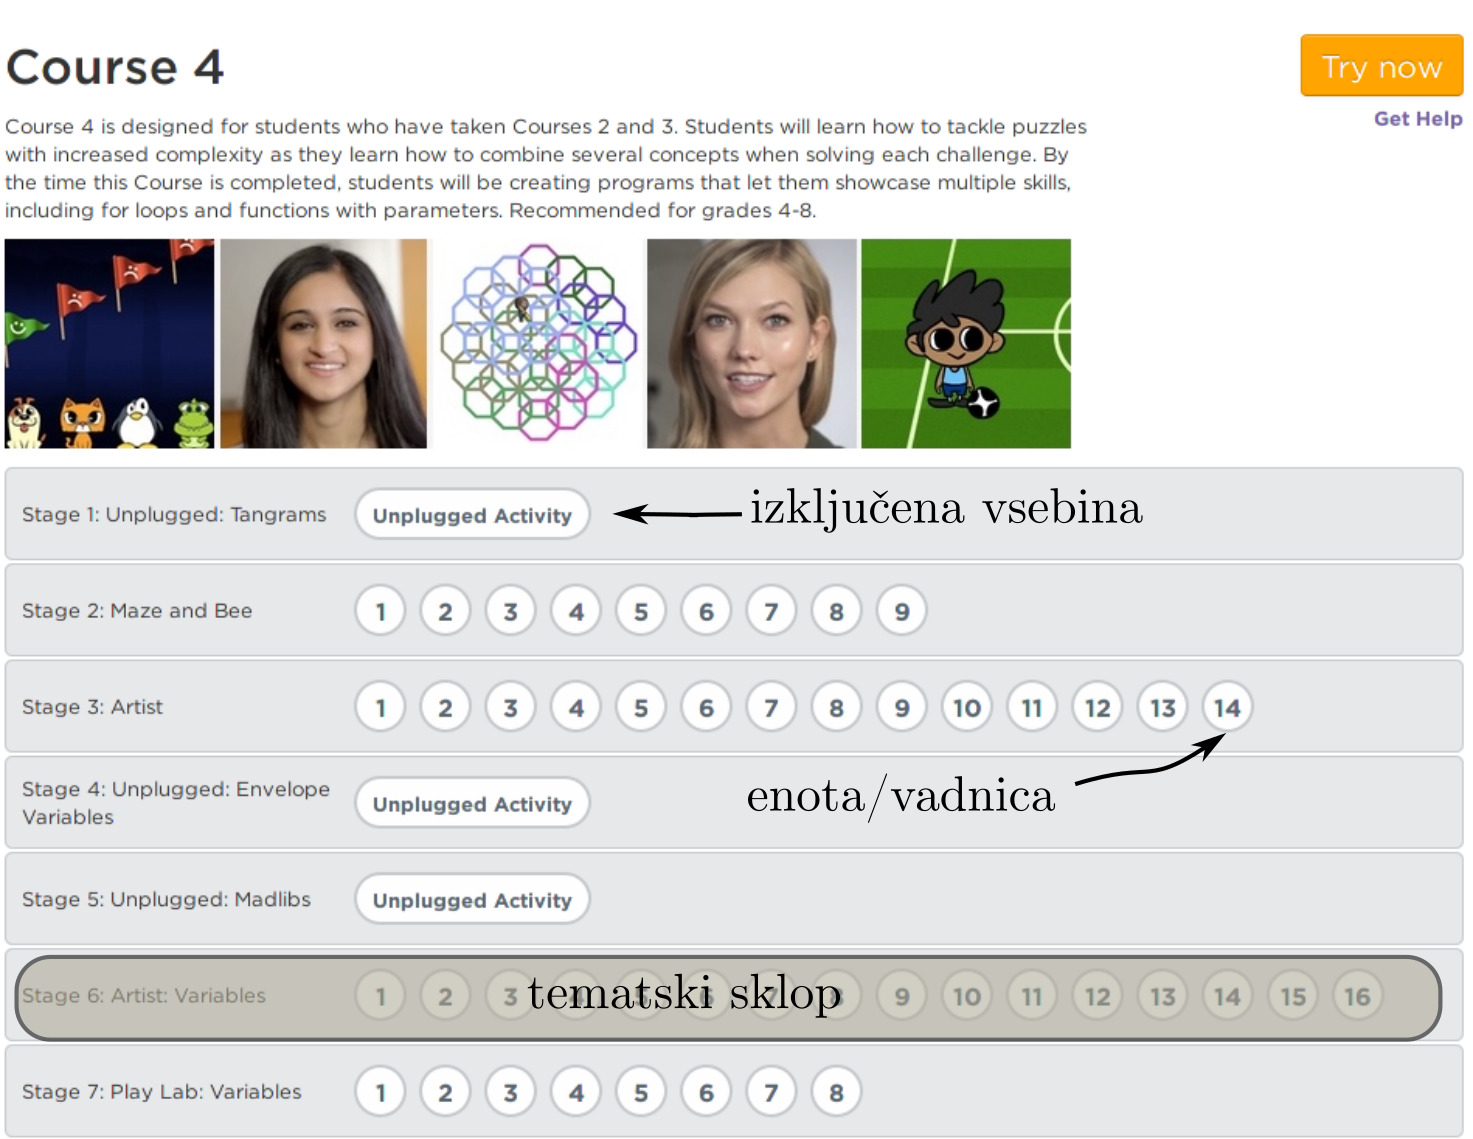
\includegraphics [width=0.65\linewidth, keepaspectratio =
  1] {./images/sc_web/code_course.jpg}
  \caption{Pod stran vsebinskega sklopa \cite{web:code.org:studio}.}
  \label{fig:scr:web:codestudio:course}
\end{figure}
  
Reševanje naloge oz. pisanje programa poteka na podoben način kot smo
ga že predstavili pri enotah \textbf{Ure kode}, vendar je teh enot več
in na vsaki naslednji enoti ponujajo več gradnikov.

\subsubsection{Samostojni projekti}
\label{sec:gradnja-projektov}

Čeprav nekoliko skrito na dnu pod strani \textbf{Code studio} najdemo
gumb na katerem piše \emph{\textbf{Moji projekti} (ang. My
  projects}). S pritiskom na gumb preidemo na stran na kateri lahko
ustvarimo nove projekte, samodejno shranjene projekte ponovno odpremo
ali jih izbrišemo. Ustvarimo lahko naslednje nove projekte,
\textbf{nariši, ustvari igro in ustvari aplikacije}. Ti projekti, so
novi in niso omejeni z nobeno vsebino, zato imajo na voljo vse
gradnike.

\textbf{Nariši} (slika \ref{fig:code:mp:draw}) deluje na podobnem
principu kot programski jezik \textbf{Logo}. Imamo pisalo, ki pušča
sled, mi mu s programsko kodo določamo potek, barvo itd. Lahko
ustvarjamo lastne funkcije in uporabljamo že obstoječe, ki jih lahko
spreminjamo. Takšna je npr. \texttt{funkcija nariši hišo}, katere
sprejme argument \texttt{velikost}. Vsi gradniki, ki jih lahko
uporabimo so omejeni izključno na uporabo pisala. 

Podobno kot nariši uporabljamo \textbf{ustvari igro} (slika
\ref{fig:code:mp:game}). Vendar tu ne uporabljamo pisala, temveč lahko
gradimo igre in zgodbe. Na del kjer teče aplikacija lahko vstavljamo
številne pred nastavljene figure, ki se odzivajo na dogodke. Sklopi
ukazov pri obeh oblikah projektov, risanja in iger so naslednji
\textbf{akcija, dogodki, zanke, matematike, logika, funkcije in
  spremenljivke}. Kljub številnim možnostim programske logike so
omejitve še vedno prisotne, kot je na primer izbira figur, ki je
omejena, saj lastnih figur ne moremo vstavljati. Uporaba teh dveh
možnosti je namenjena predvsem osnovni šoli.

\begin{figure}[h!]
  \centering
  \begin{subfigure}[]{0.45\textwidth}
    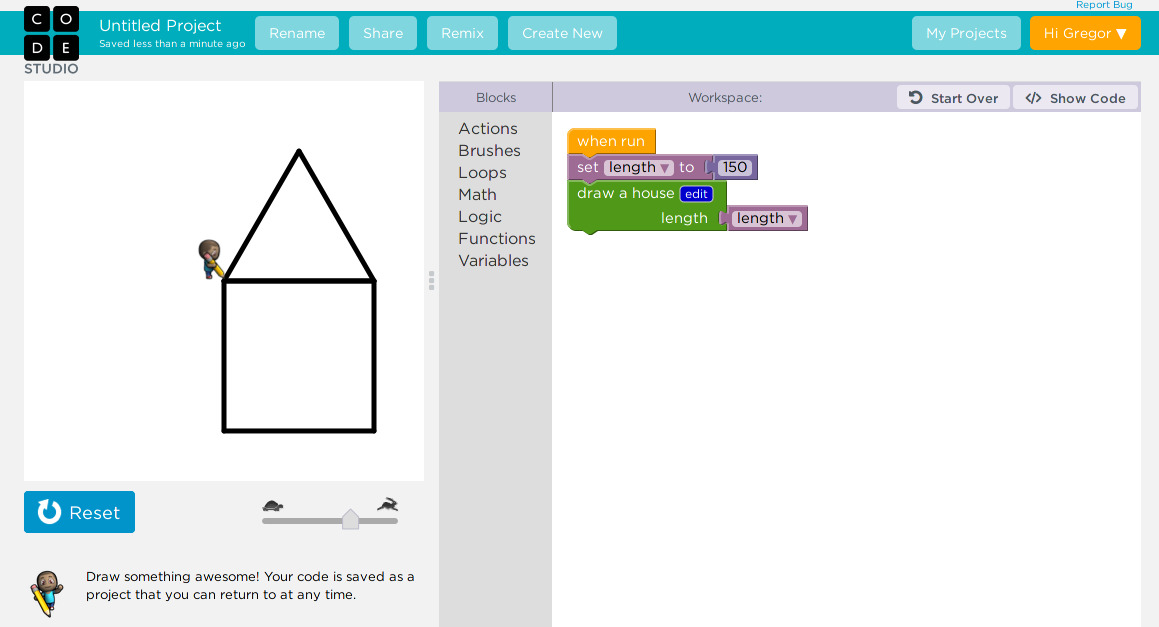
\includegraphics[width=\textwidth]{./images/sc_web/code_cs_draw.jpg}
    \caption{Aplikacija za risanje.}
  \label{fig:code:mp:draw}
\end{subfigure}
\qquad
\begin{subfigure}[]{0.45\textwidth}
  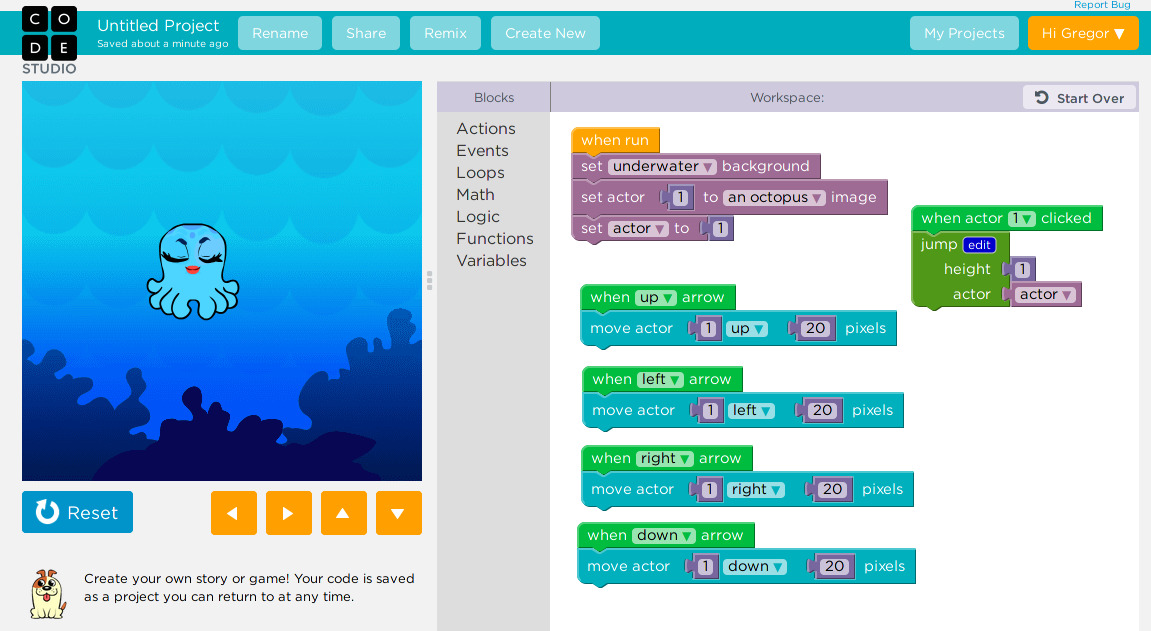
\includegraphics[width=\textwidth]{./images/sc_web/code_cs_game.jpg}
  \caption{Aplikacija za ustvarjanje iger.}
\label{fig:code:mp:game}
\end{subfigure}
\caption{Samostojni aplikaciji za programiranje primerni za
  osnovno šolo \cite{web:code.org:studio}.}
\label{fig:web:code:mp:dg}
\end{figure}

Naprednejše možnosti za programiranje smo našli v primeru
\textbf{ustvarjanja aplikacij} (slika
\ref{fig:scr:web:code:mp:app}). V tej spletni aplikaciji za
programiranje se lahko odločamo ali programsko kodo sestavljamo z
gradniki ali jo pišemo tekstovno. Glavna značilnost je ta, da poleg
pisanja programske kode moramo ustvariti še \textbf{uporabniški
  vmesnik}, ki je omejene velikosti. Sestavljanje uporabniškega
vmesnika je podobno sestavljanju mobilni aplikaciji. Z programskim
jezikom nismo več tako omejeni in lahko uporabljamo vse vgrajene
funkcije JavaScripta. Vgrajena je tudi dodatna možnost ukaznega izpisa
in osnovni pripomočki za razhroščevanje, \textbf{prekini, preskoči,
  vstopi in izstopi}.

\begin{figure}[h!]
  \centering
    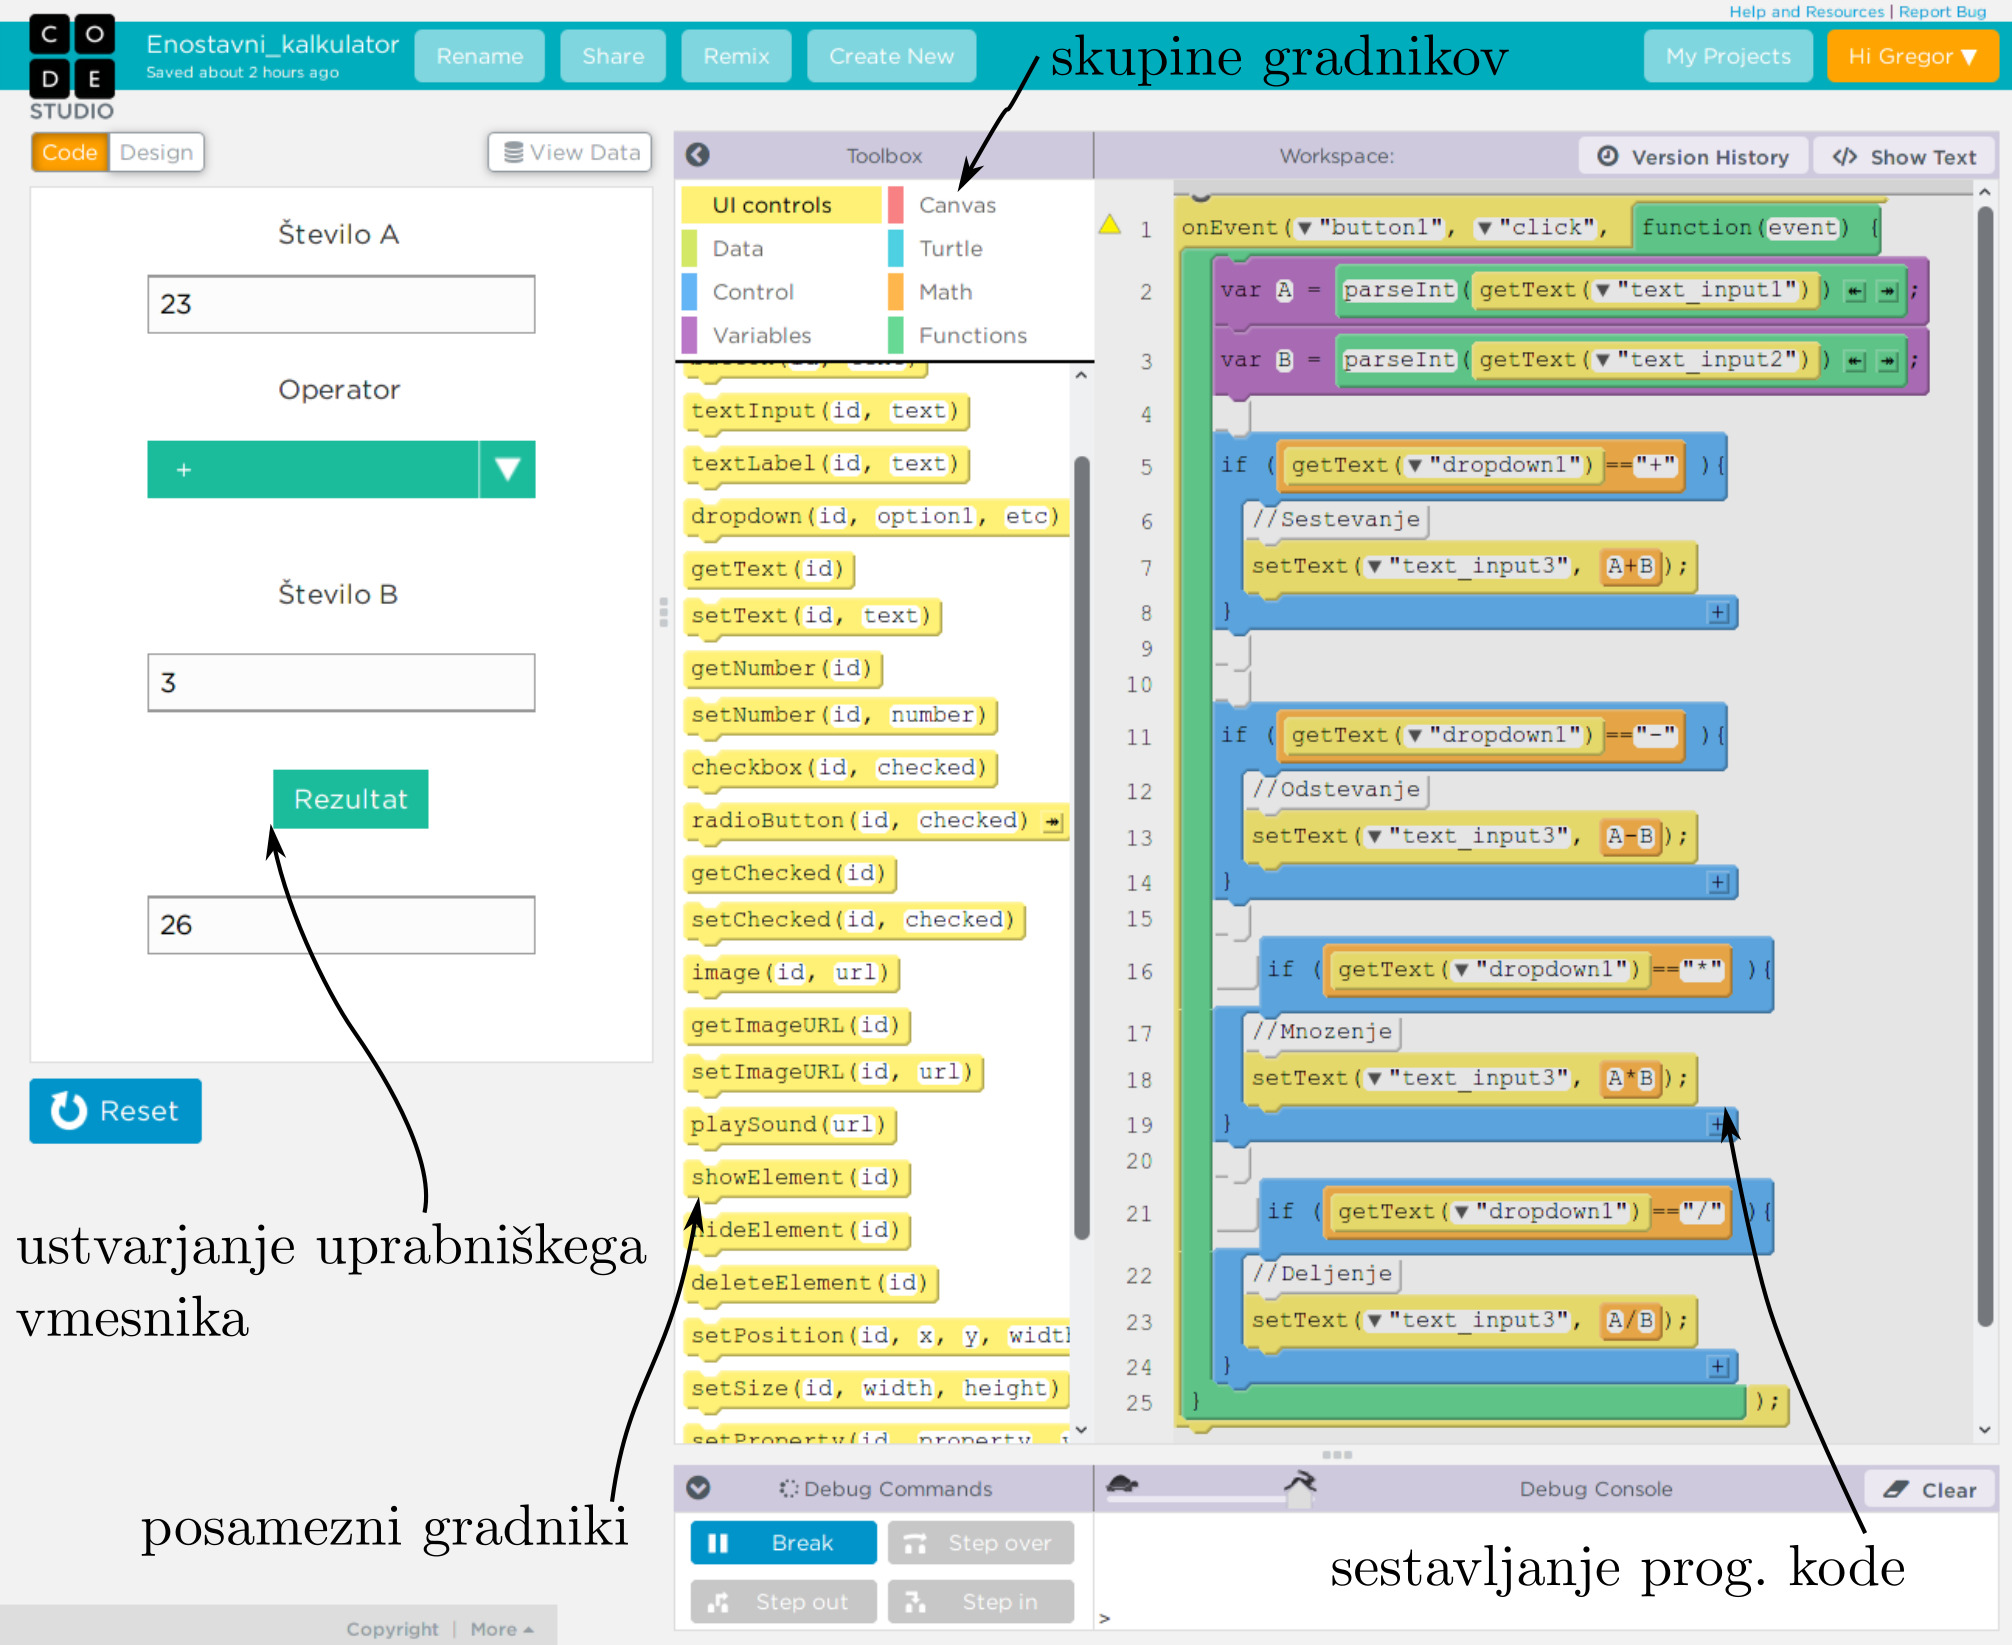
\includegraphics [width=0.90\linewidth, keepaspectratio =
    1] {./images/sc_web/code_cs_mobile.jpg}
    \caption{Spletna aplikacija za programiranje - Ustvarjanje
      aplikacij. Primer, enostavno računalo \cite{web:code.org:studio}.}
    \label{fig:scr:web:code:mp:app}
  \end{figure}

\subsubsection{Uporaba za učitelje}
\label{sec:uporaba-za-uitelje}

Celotna vsebina spletnega portala je zasnovana na ameriškem učnem
načrtu. Učitelji na strani najdejo podrobne učne načrte z cilji in
idejami za njihovo realizacijo. 

\subsubsection{Povzetek}
\label{sec:povzetek-code}

Spletni portal velja za glavnega začetnika pobude \textbf{Ure kode} in
s tem popularizaciji učenja računalniške znanosti in programiranja. Na
portalu najdemo ogromno pripravljenih in razdelanih vsebin. Primerna
je predvsem za čiste začetnike \textbf{OŠ} in jo lahko uporabljamo pri
najmlajših učencih. Za \textbf{SŠ} so pripravljene vsebine morda
prelahke in nekoliko otročje, zato jih v ta namen nebi priporočali,
čeprav zgornje omejitve vadnic ni. Vsebinski sklopi so dobro razdelani
na podrobne enote in ti postopoma stopnjujejo težavnost. Postopnost je
včasih celo pretirana in bi kakšna naloga lahko zajela dve enoti, saj
so posamezni koraki ne zahtevni oz. prelahki. Problemska zasnova je
taka, da naloge, ki je potrebno rešiti, izvajajo in rešujejo junaki z
filmskega oz. sveta video iger. To je pomembno predvsem za motivacijo
najmlajših. Nekatere vadnice so prevedene v slovenski jezik, vendar je
delež prevedenih zanemarljiv. V splošnem lahko rečemo, da večina
spletnega portala ni prevedena. Jezik uporabe spletnega portala pri
pouku nebi smel ovirati, saj so naloge razdelane na majhne dele in so
navodila enostavna, tako jih lahko učitelj podaja sproti ustno ali jih
ima pripravljene na učnih listih po posameznih korakih. Celotna
razporeditev na spletnem portalu včasih deluje ne strukturirana in
neurejena. 

Kot samostojne aplikacije v primeru \textbf{risanja in ustvarjanja
  iger} so uporabne, vendar so po zmožnostih dokaj omejene, zato lahko
v ta name z večjo svobodo in izbiro uporabljamo
Scratch. \textbf{Ustvarjanje aplikacij} je primerna predvsem za
srednje šole, omogoča pisanje programske kode, prav tako lahko
posamezne dele kode nazorno predstavimo grafično z gradniki. Uporabna
je predvsem v uvod gradnje aplikacij, saj ustvarjamo uporabniški
vmesnik in programsko kodo sami od začetka.

\begin{osebnabox}[label={osebna:codeacademy}]{Codeacademy | \url{www.codeacademy.com}}
    \begin{tabular}{
  p{0.30\linewidth-2\tabcolsep} |
  p{0.70\linewidth-2\tabcolsep}  }
  \textbf{Vrsta vsebine} & Napredna kombinirana vsebina: Vadnica
                           (video vodič + navodila(naloga) + spletna
                           aplikacija za programiranje). \\
      \hline 
  \textbf{Jezik spletne strani} &  Angleščina: da, slovenščina: da
                                  (nekatere vadnice),
                                  drugi: ne. \\
      \hline
  \textbf{Ponujena znanja} & Osnove rač. znanosti in programiranja. \\
      \hline
  \textbf{Programski jeziki} & Blocky (podobno kot Scratch),
                               JavaScript \\
      \hline
  \textbf{Težavnostna stopnja} & Osnovna šola (Vadnice, Risanje,
                                 Ustvarjanje iger), Srednja šola
                                 (Ustvarjanje aplikacij) \\
      \hline
  \textbf{Upoštevanje načel} & Upošteva načelo sistematičnosti: da,
      postopnosti: da, problemski pristop: da. \\
      \hline
  \textbf{Dosežki/Gamification} & Ne. \\
      \hline
  \textbf{Dodajanje lastnih vsebin} & Ne. \\
      \hline
  \textbf{Upravljanje razreda} & Ne. \\
      \hline
  \textbf{Dostop vsebin} & Brezplačno. \\
\end{tabular}
\end{osebnabox}

\subsection{Codeacademy}

Spletni portal je tipični predstavnik novo nastalih portalov za učenje
programiranja. Sami o sebi pravijo, da so ameriško podjetje, ki se
ukvarja z izobraževanjem. Njihov tim se z ustvarjanjem spletne strani
\emph{\href{https://www.codecademy.com/}{Codeacademy}} ter se uči in
poučuje, saj želijo ustvariti najboljšo spletno izobraževalno izkušnjo
za prihodnost, ki domuje na spletu \cite{web:codeacademy}. Po
registraciji in prijavi nas čaka naslednja spletna stran (slika
\ref{fig:scr:web:codeacademy}). Z začetne, nadzorne strani lahko
izbiramo nov vsebinski sklop ali nadaljujemo z že začetimi.

\begin{figure}[h!]
  \centering
    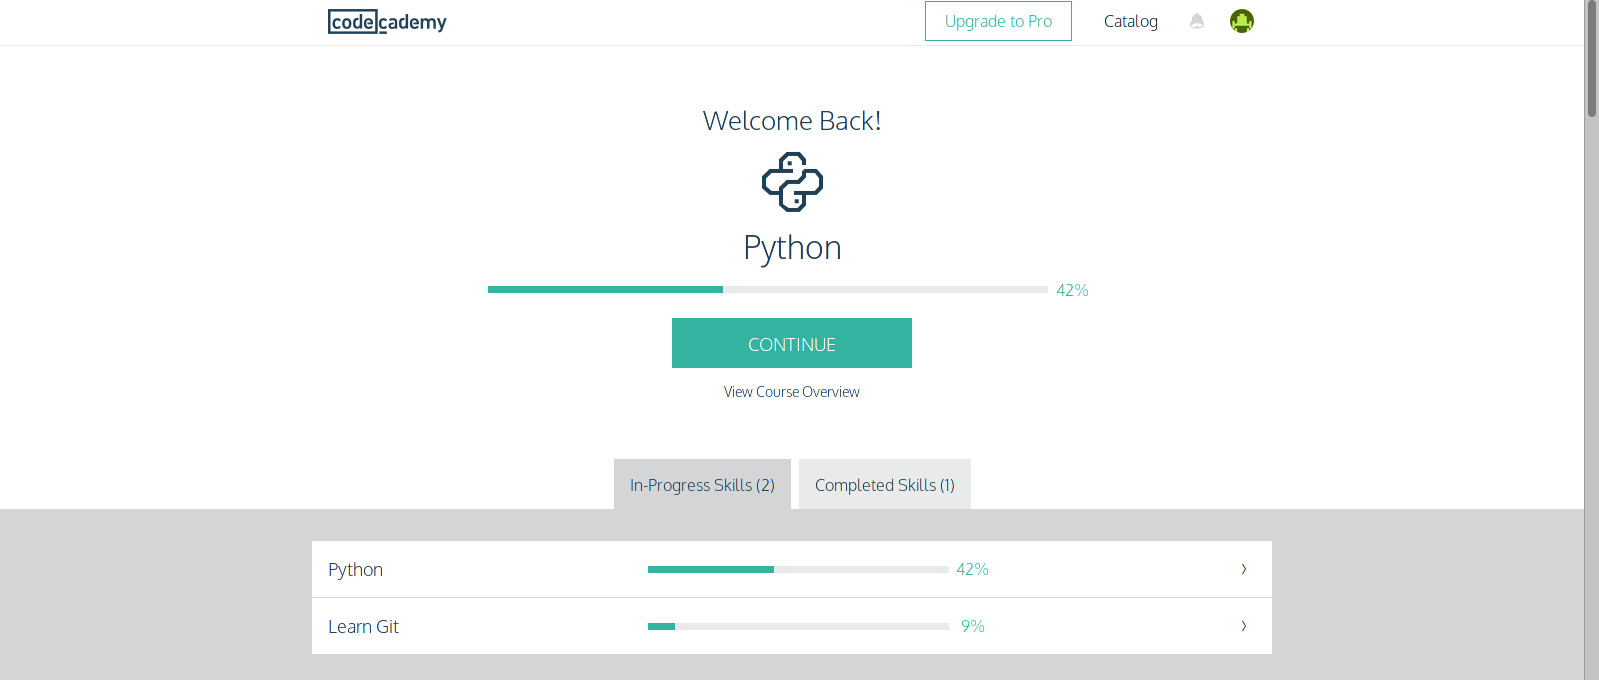
\includegraphics [width=0.65\linewidth, keepaspectratio =
    1] {./images/sc_web/codeacademy_login_01.jpg}
    \caption{Zaslonska slika spletne strani
      \emph{\href{https://www.codecademy.com/}{Codeacademy}}
      \cite{web:codeacademy}. Začetna, nadzorna stran po prijavi, od
      tu nadaljujemo na vsebinske sklope, ki smo jih že začeli.}
    \label{fig:scr:web:codeacademy}
\end{figure}

\textbf{Jezik} spletne strani je \textbf{angleščina}, drugih jezikov ni
mogoče izbrati. Če še podrsamo po spletni strani navzdol, najdemo
vsebinske sklope, ki učijo programske jezike in so naslednji: \textbf{HTML +
  CSS, JavaScript, JQuery, PHP, Python, Ruby} in že v prejšnjem odseku
so bile na voljo osnove \textbf{Jave}.

\begin{figure}[h!]
  \centering
    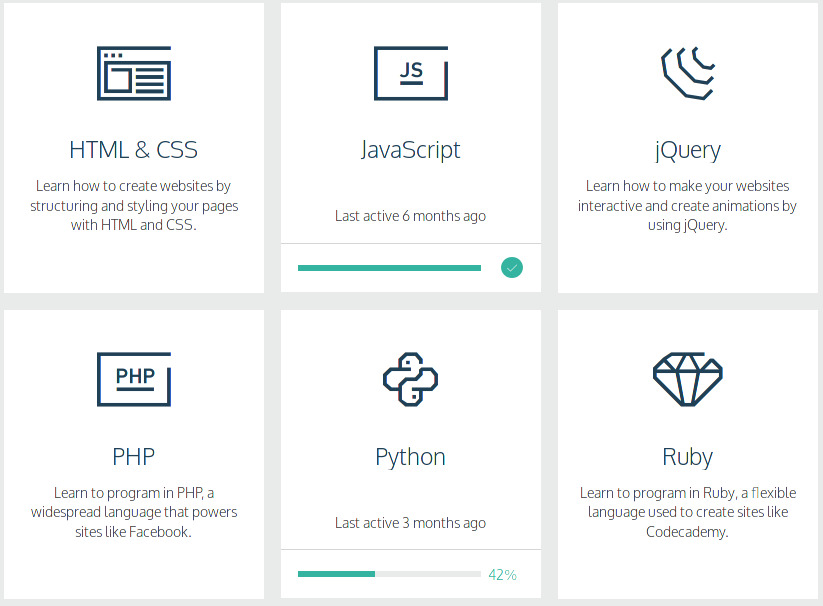
\includegraphics [width=0.65\linewidth, keepaspectratio =
    1] {./images/sc_web/codeacademy_vescine_02.jpg}
    \caption{Zaslonska slika spletne strani
      \emph{\href{https://www.codecademy.com/}{Codeacademy}}
      \cite{web:codeacademy}. Seznam znanj/veščin programskih jezikov,
      ki jih ponuja spletni portal.}
    \label{fig:scr:web:codeacademy:vescine-prog}
\end{figure}

Nad zbirko osnovnih programskih jezikov najdemo druga
\textbf{ponujenih znanj}. V tem delu najdemo nekatere vsebine kot je
na primer, učenje \textbf{SQL}, uporaba \textbf{ukazne vrstice} ali
uporabo spletnega orodja za kontrolo verzije \textbf{GIT}. Nekatere
vsebine so sestavljene kot projekti, taki sta na primer \textbf{Naredi
  spletno stran} ali \textbf{Naredi spletno stran interaktivno}. 
Strnemo lahko, da spletni portal ne ponujajo le znanja in veščine
\textbf{programiranja in programskih jezikov}, temveč tudi druga
znanja. S klikom na želeno vsebino pridemo na stran (slika
\ref{fig:scr:web:codeacademy:tema}), s katere lahko nadaljujemo tam
kjer smo ostali ali pregledujemo posamezne teme, ki smo jih že
opravili ali tiste, ki nas še čakajo.


% \begin{figure}[h!]
%   \centering
%     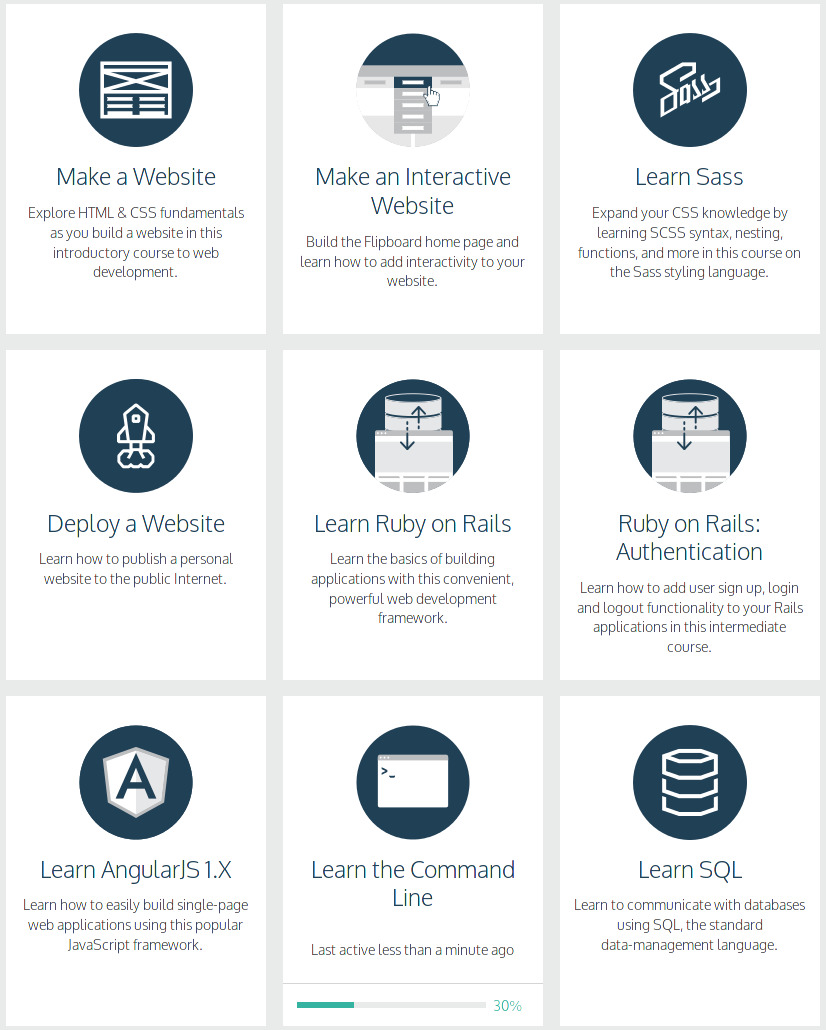
\includegraphics [width=0.65\linewidth, keepaspectratio =
%     1] {./images/sc_web/codeacademy_vescine_01.jpg}
%     \caption{Zaslonska slika spletne strani
%       \emph{\href{https://www.codecademy.com/}{Codeacademy}}
%       \cite{web:codeacademy}. Seznam znanj/veščin, ki jih ponuja
%       spletni portal.}
%     \label{fig:scr:web:codeacademy:vescine-web}
% \end{figure}

\begin{figure}[h!]
  \centering
    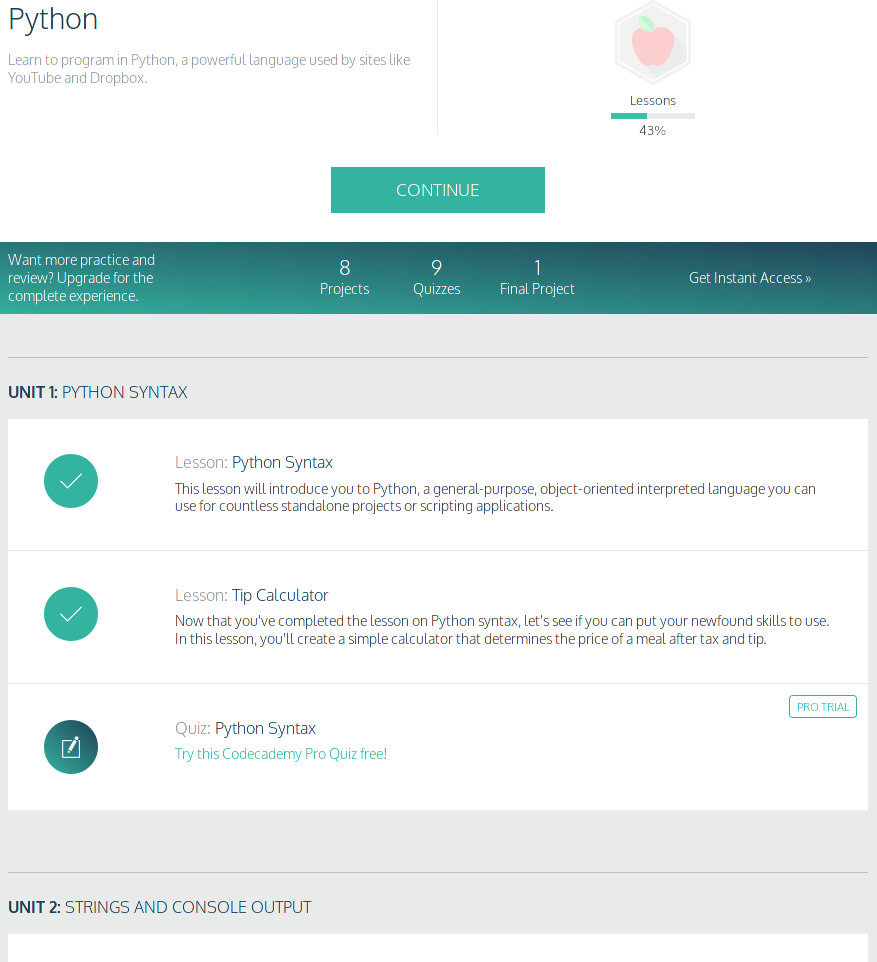
\includegraphics [width=0.65\linewidth, keepaspectratio =
    1] {./images/sc_web/codeacademy_tema_01.jpg}
%  \def\svgwidth{\columnwidth}
%  \input{./pdf_tex/codeacademy_tema_01.pdf_tex}
  \caption{Zaslonska slika pod strani spletne strani
      \emph{\href{https://www.codecademy.com/}{Codeacademy}}
      \cite{web:codeacademy} na kateri lahko pregledujemo posamezne
      teme in nadaljujemo tam, kjer smo ostali.}
    \label{fig:scr:web:codeacademy:tema}
\end{figure}

Razvidno je, da so teme sistematično razporejene, zato lahko ugotovimo
da je \textbf{načelo sistematičnosti upoštevano}. Z pritiskom na gumb
za nadavaljevanje (\emph{ang. Continue}) odpremo urejevalnik (slika
\ref{fig:scr:web:codeacademy:ide}) na temi in pod enoti na kateri smo
ostali.

\begin{figure}[h!]
  \centering
    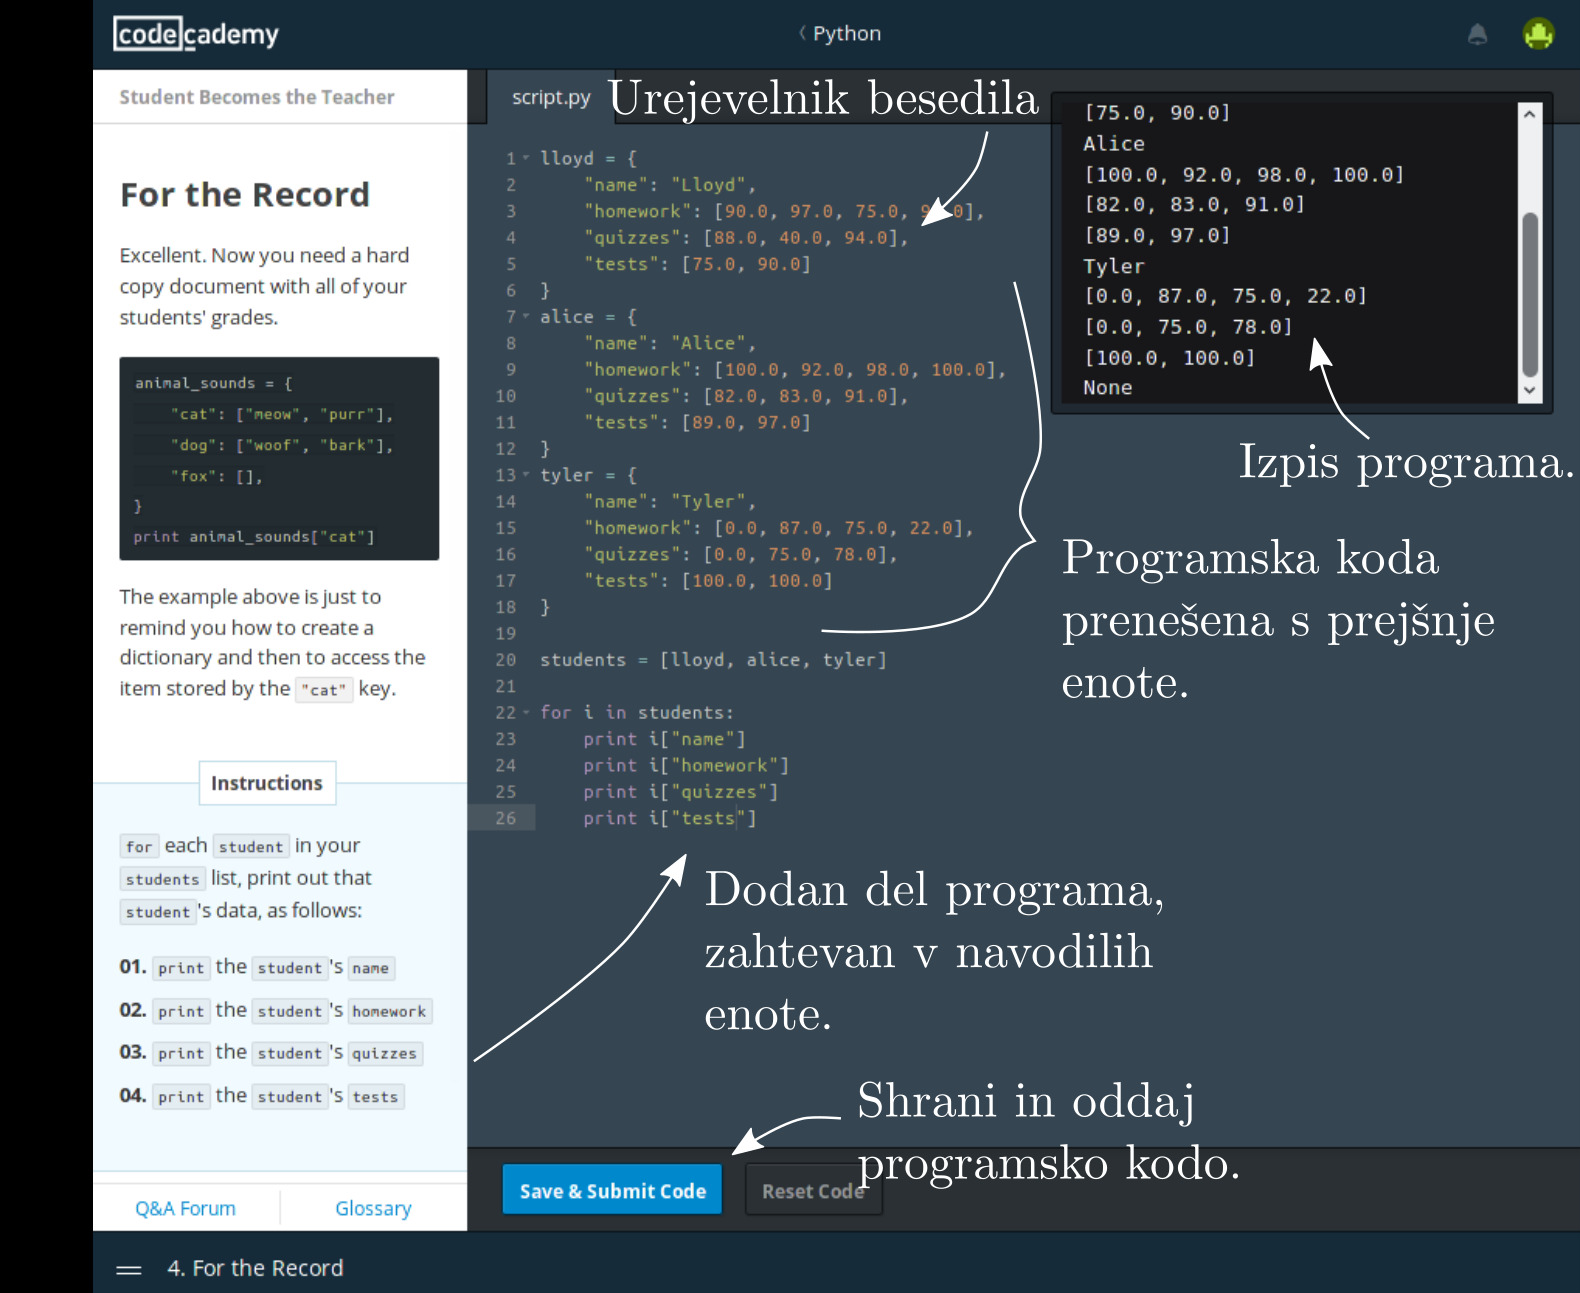
\includegraphics [width=0.65\linewidth, keepaspectratio =
   1] {./images/sc_web/codeacademy_IDE_02.jpg}
   \caption{Zaslonska slika
     \emph{\href{https://www.codecademy.com/}{Codeacademy}}
     \cite{web:codeacademy} vadnice, ki jo sestavlja urejevalnika z
     navodili in oknom za izpis v programu.}
    \label{fig:scr:web:codeacademy:ide}
\end{figure}

Vsaka tema vsebinskega sklopa je razdeljena na več enot oz. vadnic, ki
so sestavljene tako, da postopoma dograjujejo program. Delo, ki smo ga
opravili v predhodni vadnici se samodejno prenese naprej, ko je to
potrebno. Lahko povemo, da je \textbf{načelo postopnosti
  upoštevano}. Pri nekaterih tematskih sklopih sledi najprej ponovitev
že naučenega. Na primer pri Temi \emph{Seznami in funkcije} najprej
sledi pregled osnovnega upravljanja z seznami in pisanjem funkcij.
Uporabniški vmesnik (slika \ref{fig:scr:web:codeacademy:ide}) je
urejen tako, da na desni strani imamo podano snov, ki je sestavljena s
\textbf{primerom določene programske strukture in navodili}, kaj
moramo dograditi v programu. Na levi strani imamo \textbf{urejevalnik
  besedil} v katerega pišemo programsko kodo. Urejevalnik zna barvati
programsko kodo in samodejno predviditi zamike besedila. V zgornjem
desnem kotu je \textbf{okno za izpis} v katerem se izpisujejo
\textbf{izhodni podatki} s programa in napake sintakse \textbf{Pyton
  tolmača}. Spodaj je gumb za \textbf{Shrani in oddaj programsko kode}
(\emph{ang. Save and Submit Code}).

Vsaka v uvodnem delu predstavi novo problematiko, ki jo potem čez
posamezne enote rešujemo. Vsebina je predstavljena
\textbf{problemsko}. Samo delo z \textbf{vadnico} poteka tako, da
napišemo program v \textbf{spletno aplikacijo za programiranje}, ki je
zahtevan v navodilih. Ko menimo, da imamo pravilno rešitev pritisnemo
na gumb \textbf{Shrani in oddaj programsko kodo.} Program najprej
preverja \textbf{sintaktično} pravilnost. Napako program vrne nad
gumbom za oddajo programske kode, podrobna napaka \textbf{Python-ovega
  tolmač} se izpiše v \textbf{oknu za izpis}. Zatem sledi
\textbf{semantično} preverjanje pravilnosti rešitve naloge. V
posamezni enoti program samodejno vrši osnovno preverjanje programa, z
točno določenim rezultatom. Dokler test napisanega programa ne da
pravega rezultata me moremo nadaljevati na naslednjo enoto. Ko se nam
zatakne, spletna stran ponuja \textbf{forum} na katerem najdemo
odgovor ali lahko postavimo vprašanje. Forum je razdeljen na posamezne
teme in enote, tako da lahko hitro najdemo zahtevano vprašanje.

%Zbiranje dosežkov
Za uspešno premagovanje enot je uporabnik nagrajen z
\textbf{značkami}, ki so vidne na strani njegovega profila. Na tej
strani se beležijo tudi predelane vsebine. Spletni portal torej
uporablja nagrajevanje z \textbf{dosežki}.

Spletni portal ponuja tudi plačljive vsebine, čeprav je osnova
vsebinskih sklopov brezplačna. Za dostop do plačljivih storitev, za
ponujajo model zakupa z naročnino za ceno \textbf{19\$/mesec}. Za
naročnino uporabnik pridobi dostop do\textbf{ naslednjih dodatnih
  storitev}:

\begin{itemize}
\item personaliziran učni načrt;
\item dostop do kvizov;
\item dostop do realnih projektov;
\item dostop pomoči v živo preko sporočil.
\end{itemize}

Ugotovimo, da je spletni portal \textbf{pol plačljivi} in da dodatne
storitve, ki jih ponuja spletni portal niso potrebne za uporabo pri
pouku, saj vse omenjene dodatne storitve lahko zagotovi učitelj.

\subsubsection{Uporaba za učitelje}
\label{sec:uporaba_učitelji}

Spletni portal nudi vsebine, ki so prilagojene za šole in uporabo v
šolah. V pregledu lahko ugotovimo, da za srednješolske profesorje
ponujajo naslednje:

\begin{itemize}
\item \textbf{trening za učitelje}, ki je možen le v ZDA;
\item \textbf{gradiva};
\item \textbf{sledenje napredku učencem};
\item \textbf{ura kode} (ang. \emph{Hour of code}).
\end{itemize}

Pod stran z \textbf{ gradivi} %(slika \ref{fig:scr:web:codeacademy:tr})
profesorju ponuja razdelane posamezne teme na enote podobno kot so
razdelane na glavni strani. Pod vsako enoto profesor lahko preizkusi,
rešuje vaje. Večina enot ima pripravljene kvize, ki jih profesor lahko
prav tako preizkusi in se pripravi na učno uro.

% \begin{figure}[h!]
%   \centering
%     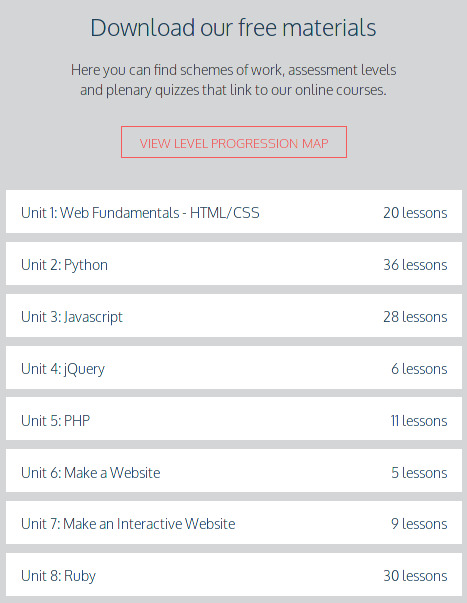
\includegraphics [width=0.40\linewidth, keepaspectratio =
%    1] {./images/sc_web/codeacademy_tr_01.jpg}
%    \caption{Zaslonska slika
%      \emph{\href{https://www.codecademy.com/}{Codeacademy}}
%      \cite{web:codeacademy} pod strani z gradivi in tematskimi
%      sklopi.} %%NI ukazna vrstica temveč ...
%     \label{fig:scr:web:codeacademy:tr}
% \end{figure}

Kot so si zamislili avtorji spletnega portala so tematski sklopi in
posamezne enote med seboj prepletene in vodijo do posameznega
cilja. Zemljevid (slika \ref{fig:codeacademy:poster}) prikazuje
povezavo enot na posamezni stopnji in različne cilje. Za vsak tematski
sklop učitelj lahko prenese \textbf{pregled posamezne teme}, v kateri
so podrobneje zapisani učni cilji in so označene stopnje ki sovpadajo
z zemljevidom.

\begin{figure}[h!]
  \centering
    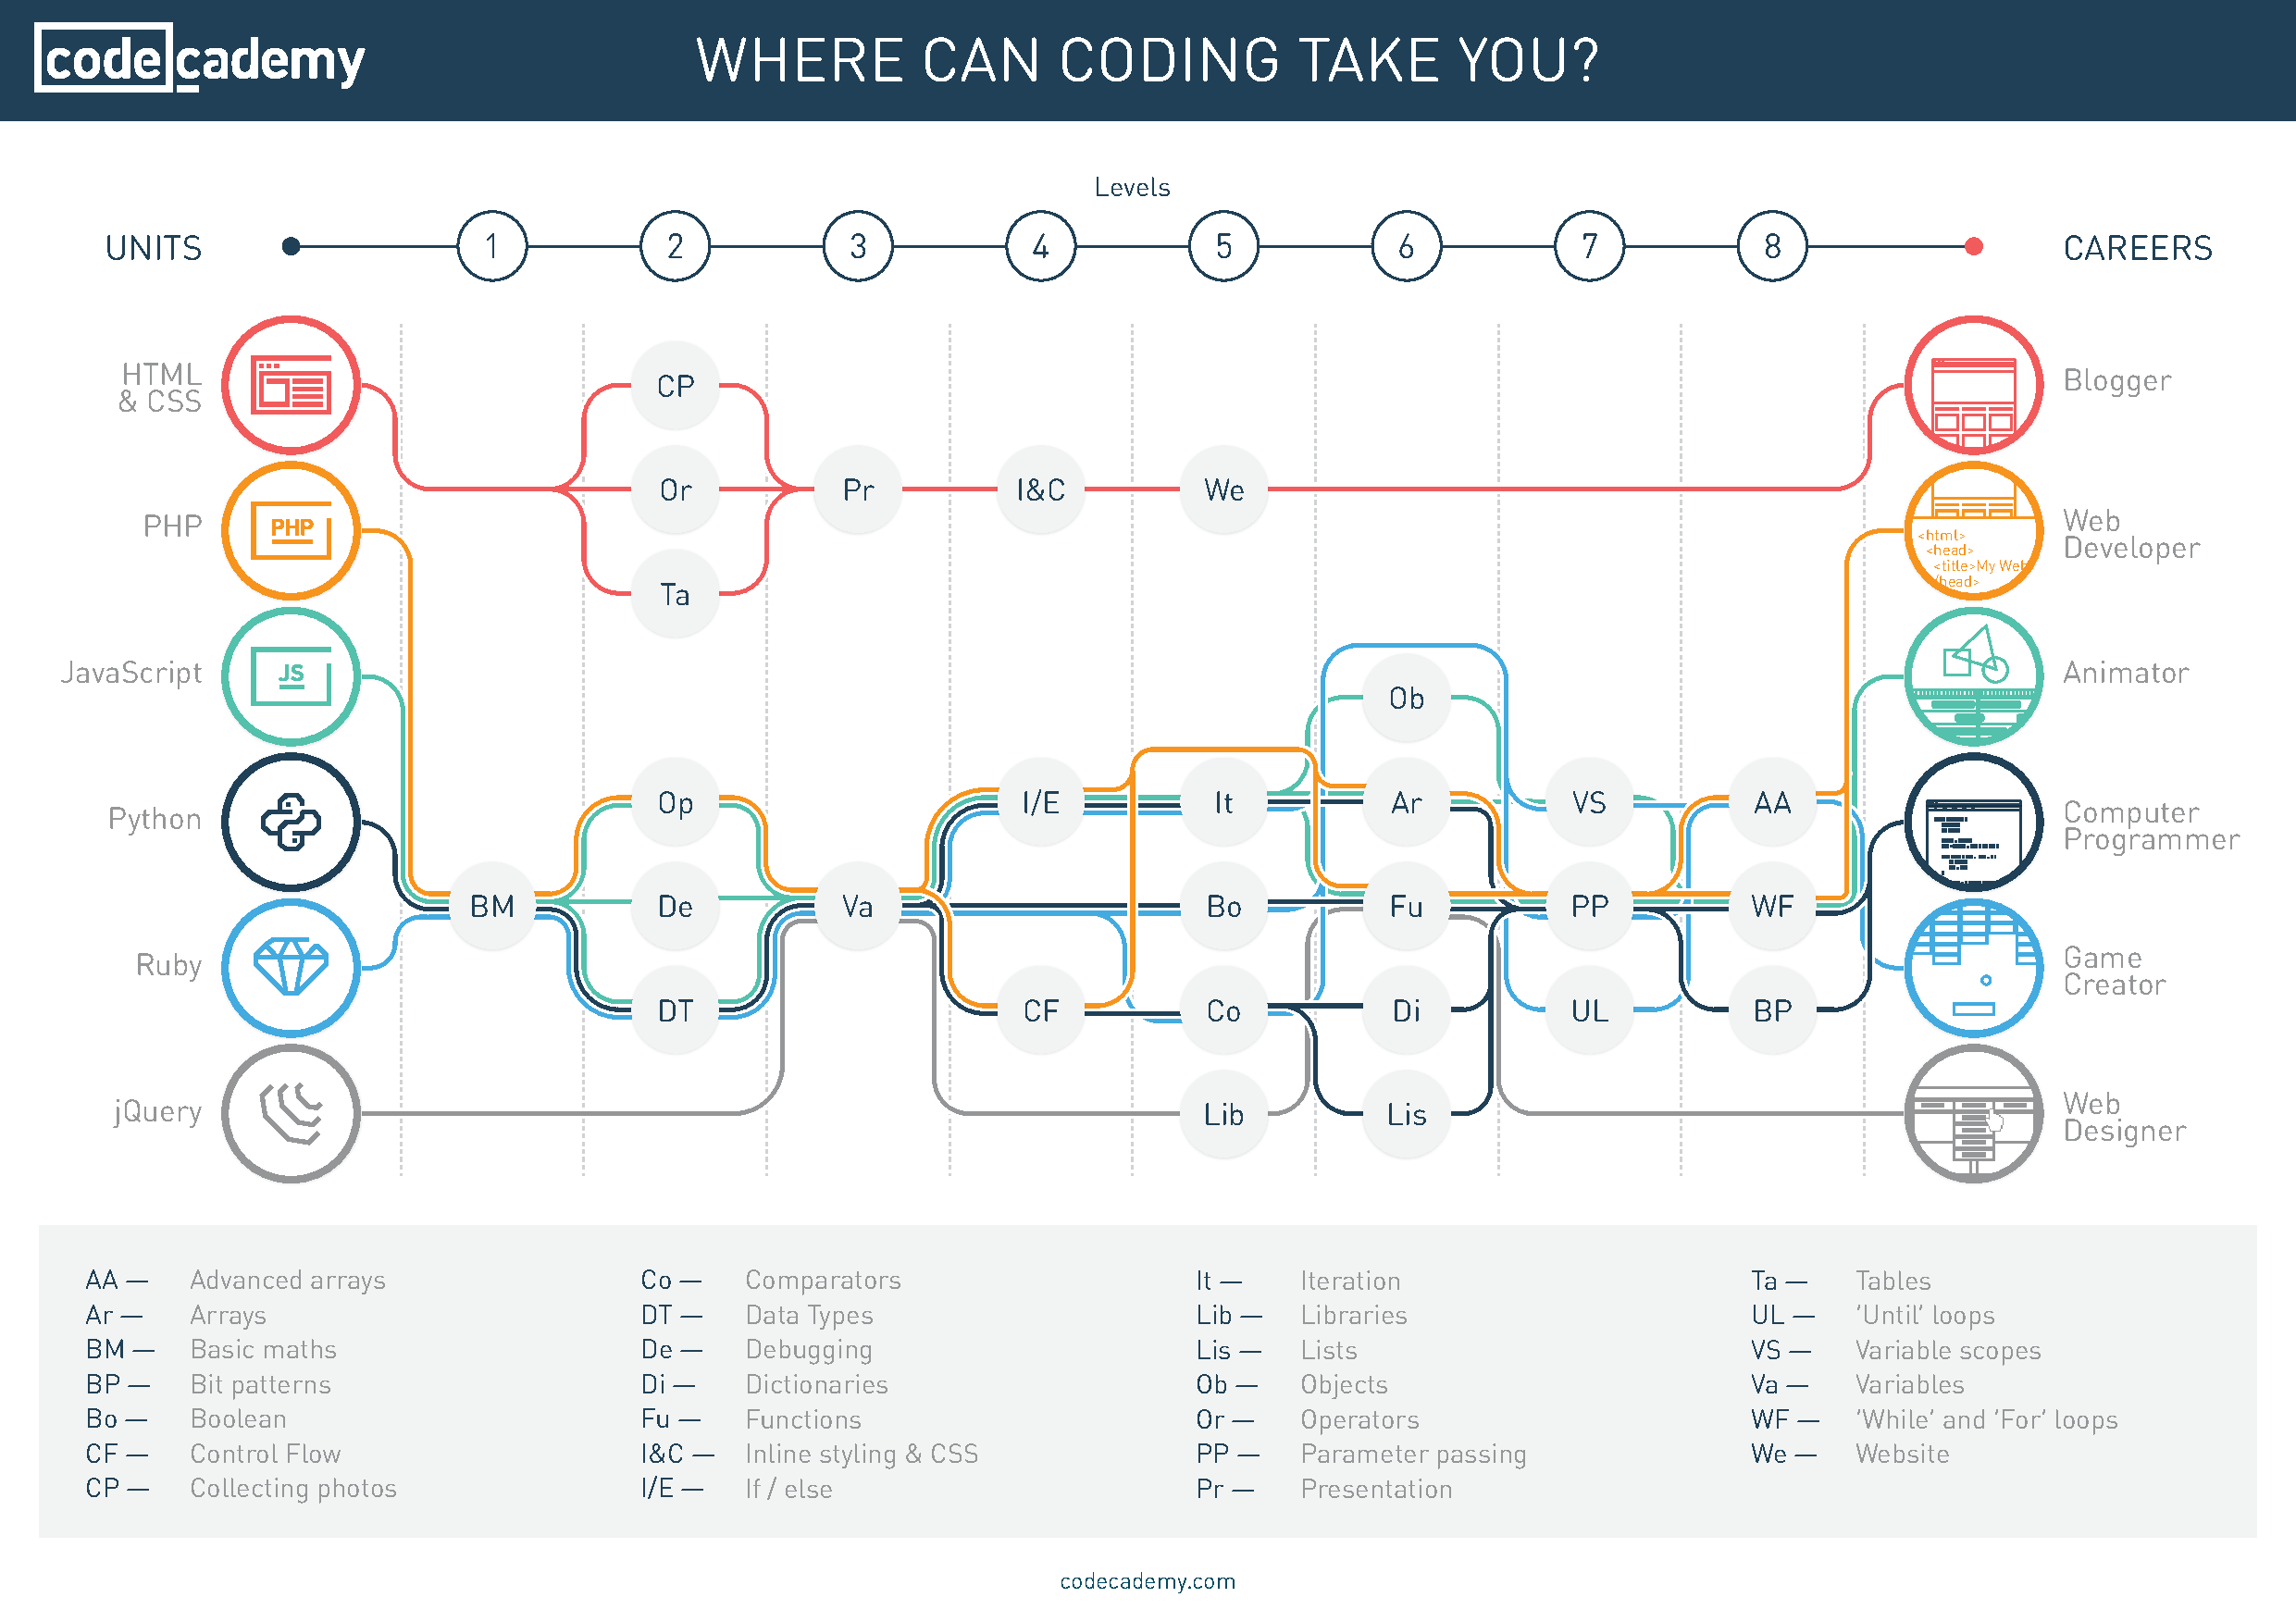
\includegraphics [width=1\linewidth, keepaspectratio =
   1] {./images/CAdemy-poster.pdf}
   \caption{Plakat z povezavami enot različnih tematskih sklopov po
     stopnjah, ki vodijo  do posameznih ciljev (\emph{ang. Level
       prograsion mapa}) \cite{web:codeacademy}.}
    \label{fig:codeacademy:poster}
\end{figure}

Ena izmed naprednih zmožnosti spletnega portala je \textbf{sledenje
  napredku učencem} (\emph{ang. Students tracking}). Ta omogoča, da
profesor dijakom ustvari račune in jih povabi na spletnem portalu v
razred. Določi tematske sklope katerim bo sledil. V pregledu (slika
\ref{fig:scr:web:codeacademy:tracking}) profesor lahko opazuje
napredek posameznega dijaka po enotah ali v povzetku za celotni
napredek. Napredek je prikazan z pikami različnih barv, ki
predstavljajo procente napredka pri posameznem tematskem sklopu. V tem
primeru \textbf{ne moremo} govoriti o \textbf{upravljanju razreda},
saj omogočeno le sledenje napredku in ne tudi komunikacija med
profesorjem in dijakom, prav tako ni mogoče dodajati lasnih enot
oz. nalog. Pri samem ustvarjanju razreda, je profesorju delo zelo
olajšano, saj portal omogoča, da informacije o dijakih ustvarjalec
razreda kopira direktno s programa podobnega kot je \textbf{Excel}. V
tabeli so podani podatki \textbf{ime, priimek, skupina, uporabniško
  ime}. Dijaki za dostop do spletnega portala uporabijo uporabniško
ime, ki si ga izmisli učitelj ali oni sami, geslo je skupno za celotno
učilnico. Z prejetim uporabniškim imenom in geslom se dijaki na
spletni strani registrirajo z svojim email naslovom. Če so na portalu
že registrirani profesorju posredujejo uporabniško ime in jih ta doda
v ustvarjen razred. Dijak mora povabilo potrditi.

\begin{figure}[h!]
  \centering
    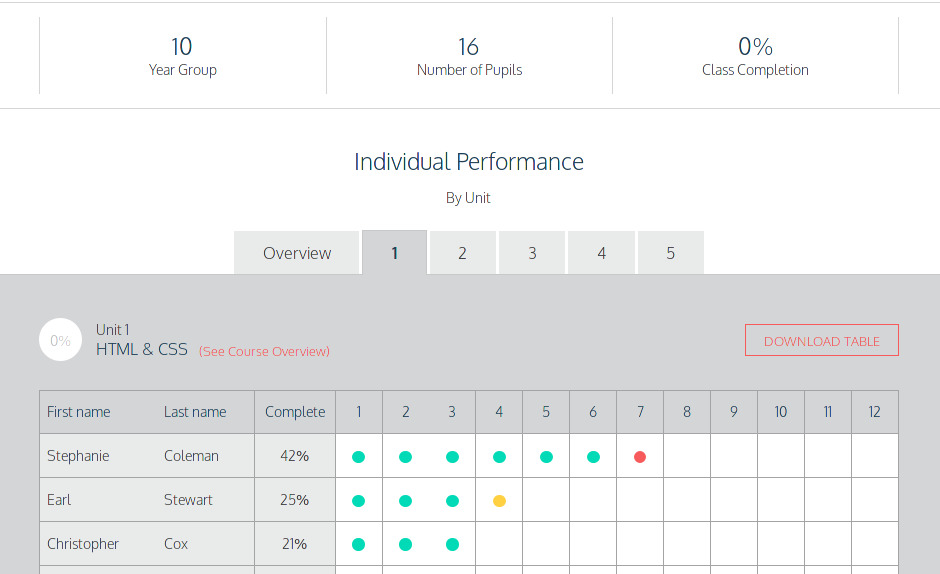
\includegraphics [width=0.65\linewidth, keepaspectratio =
   1] {./images/sc_web/codeacademy_tracking_01.jpg}
   \caption{Zaslonska slika
     \emph{\href{https://www.codecademy.com/}{Codeacademy}}
     \cite{web:codeacademy}. Prikazuje tabelo za sledneje napredku
     učencem.}
    \label{fig:scr:web:codeacademy:tracking}
\end{figure}

\subsubsection{Povzetek}

\emph{\href{https://www.codecademy.com/}{Codeacademy}}
\cite{web:codeacademy} ima dobro razdelano vsebino, ki je na nekaterih
delih dokaj poglobljena. Sistematičnost, postopnost in problemski
pristop sta prav tako dobro zastavljeni. Portal ponuja številne
projektne vsebine in učenje programskih jezikov. Izbor teh je tak, da
ustreza današnjim spletnim tehnologijam in zahtevam. Znanje se omejuje
predvsem na učenje programiranja ter da se to znanje zna uporabiti v
praktične namene. Spletni portal ima nekatere vsebine in zmožnosti
plačljive, ampak ima zadostno število brezplačnih vsebin, ki omogočajo
normalno učenje. 

Zanemarjeno je znanje \textbf{Računalniške znanosti}, saj se med
spoznavanjem programskih jezikov in podatkovnih struktur ne uči
različnih algoritmov. Uči se bolj uporabo posameznih funkcij, ki so
vgrajene v programski jezik. Slaba stran spletnega portala je ta, da
je ves v \emph{angleškem jeziku}. Poleg tujega jezika so nekatera
navodila napisana dokaj kompleksno in zahteva že dobro poznavanje
razumevanja sporočil tolmača in semantičnih napak, ki se zgodijo v
programu.

Spletni portal je v primeru učenja spletnih tehnologij, kot je
\textbf{HTML/CSS} je primeren za učence zadnje triade osnovne šole,
saj se ti omenjeno snov učijo pri izbirnem predmetu
\textbf{Računalniška omrežja}. V primeru učenja programskega jezika
\textbf{Python} spletni portal ponuja zahtevna znanja in je primeren
predvsem za srednje in višje šole.

Da bi mentor lahko spletni portal uporabljal pri pouku bi moral imeti
prevode navodil za posamezno temo in enoto. Vsekakor je možno izvesti
kot \emph{praktično vodeno delo}. Spletni portal se lahko uporablja za
domače delo in smo uporabo kot takega opisali v poglavju
\ref{sec:prim-uresn-cil-ss}. Mentor lahko, spletni portal priporoča v
uporabo, kot za neobvezno dopolnilno dejavnost tistim, dijakom, ki
želijo razširiti znanje programiranja. Opozorimo, da jim lahko
priporoča le brezplačne vsebine. Čeprav je možno, pa vseeno morda ni
primerno uporabljati spletni portal tako, da bi z njim predelali
celoten vsebinski sklop in bi ga pri pouku uporabljali kot edino
orodje, saj je poučevanj računalniške znanosti na njem omejeno. Lahko
ga pa s pridom uporabimo kot dodatek pri učenju programskega jezika,
kot je na primer \textbf{Python}, ki v nadaljevanju služi kot orodje
za poučevanje računalniške znanosti.  Pri pouku smo omejeni tudi s
spreminjanjem vsebine, ki je ni mogoče prilagoditi k učnemu načrtu
tako kot bi to želeli, zato moramo učno pripravo prilagoditi uporabi
spletnega portala. Poleg prednosti in slabosti lahko zaključimo, da
ima spletni portal še dodatno motivacijsko vrednost, saj njegova
sistematičnost in postopnost ter nagrajevanje z dosežki motivira
uporabnike, da imajo željo po dokončanju vsebinskega sklopa, ki ga
obravnavajo. 

\begin{osebnabox}[label={osebna:codeacademy}]{Codeacademy | \url{www.codeacademy.com}}
    \begin{tabular}{
  p{0.30\linewidth-2\tabcolsep} |
  p{0.70\linewidth-2\tabcolsep}  }
  \textbf{Vrsta vsebine} & Napredna kombinirana vsebina: Vadnica
                           (primer +  navodilo(vodič) + spletna
                           aplikacija za programiranje).  \\
      \hline
  \textbf{Jezik spletne strani} &  Angleščina: da, slovenščina: ne,
                                  drugi: ne. \\
      \hline
  \textbf{Ponujena znanja} & Znanje prog. jezikov, druge vsebine. \\
      \hline
 \textbf{Programski jeziki} & \textbf{HTML+ CSS}, Java JavaScript, Jquery, PHP,
                              \textbf{Python}, Ruby \\
      \hline
  \textbf{Težavnostna stopnja} & 3/3 Osnovna šola, Srednja šola. \\
      \hline
   \textbf{Upoštevanje načel} & Upošteva načelo sistematičnosti: da,
      postopnosti: da, problemski pristop: da. \\
      \hline
  \textbf{Dosežki/Gamification} & Da (značke). \\
      \hline
  \textbf{Dodajanje lastnih vsebin} & Ne. \\
      \hline
  \textbf{Upravljanje razreda} &Da, ustvarjanje razreda in sledenje
                                 napredku učencem. \\
      \hline
  \textbf{Dostop vsebin} & Pol plačljiv (plačljivi so projekti, kvizi,
                           podpora v živo). \\
\end{tabular}
\end{osebnabox}

\subsection{Scratch}
\label{sec:scratch}

Spletni portal \emph{\href{https://scratch.mit.edu/}{Scratch}}
\cite{web:scratch} je spletna različica zelo popularnega programskega
jezika \textbf{Scratch}. Scratch je pri nas popularen predvsem v
\textbf{osnovnih šolah} in je zamenjal dolgo uporabljen \textbf{Logo}.

Razvoj samostojne namizne različice Scratcha se je končala pri verzi
1.4, od tu naprej je razvoj Scratcha potekal za spletno
različico. Spletna različica je narejena na osnovi zaprtega
\textbf{Adobe Flash}. Za poganjanje Scratch v spletnem brskalniku
potrebujemo vtičnik \textbf{Flash}. Ko prvič naložimo spletni portal
\emph{\href{https://scratch.mit.edu/}{Scratch}} (slika
\ref{fig:web:scratch:main}) lahko ugotovimo, da ponuja naslednje
funkcionalnosti:

\begin{itemize}
\item ustvarjanje programov (Orodje Scratch);
\item deljenje ustvarjenih programov;
\item raziskovanje narejenih programov, drugih uporabnikov;
\item forum za diskusije;
\item pomoč pri uporabi
\end{itemize}

\begin{figure}[h!]
  \centering
    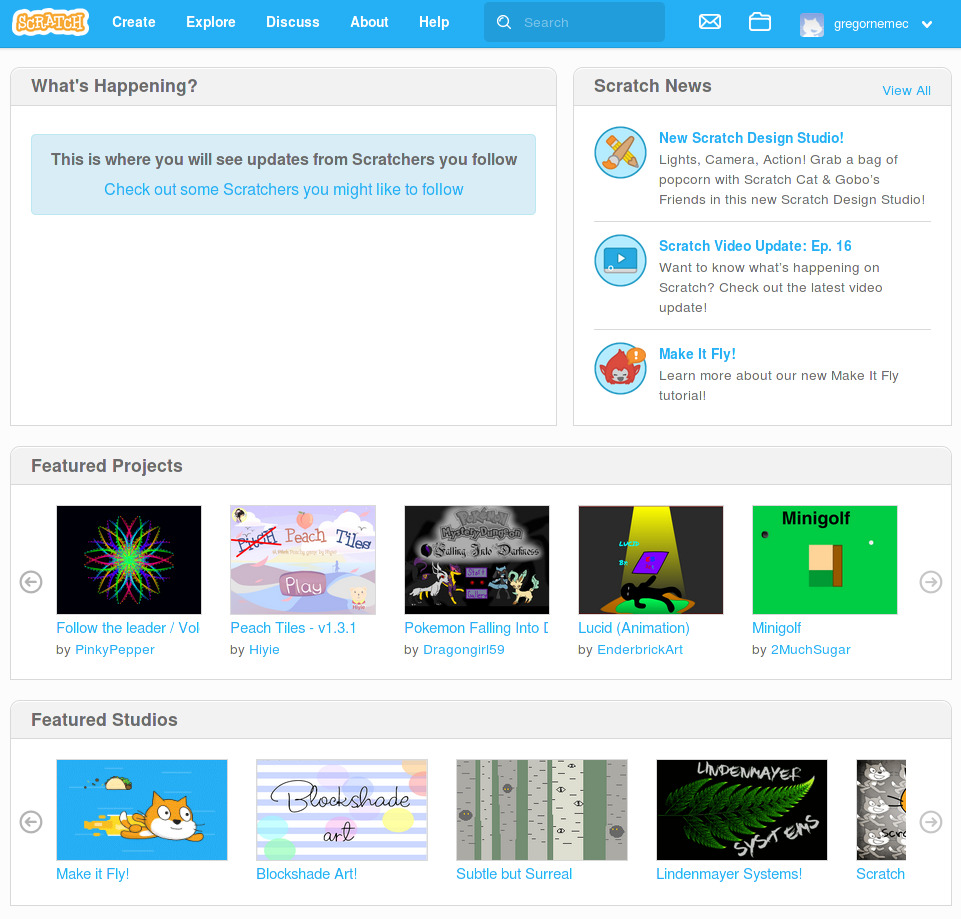
\includegraphics [width=0.65\linewidth, keepaspectratio =
   1] {./images/sc_web/scratch_mainP-v01.jpg}
   \caption{Zaslonski posnetek glavne strani
     \emph{\href{https://scratch.mit.edu/}{Scratch}}
     \cite{web:scratch}.}
    \label{fig:web:scratch:main}
\end{figure}

Scratch smo po vrsti vsebine umestili med \textbf{spletne aplikacije
  za programiranje} oz. smo ga predstavili kot samostojno
\textbf{orodje}. Lastne vsebine, ki bi v širšem smislu poučevala
računalniško znanje ne najdemo. Vse vsebin, ki so na strani, so
namenjene učenju uporabe orodje in spoznavanjem zmožnosti programskega
jezika. Govorimo lahko vseeno o spletnem portalu, saj ta ima vse za
uspešno uporabo orodja in omogoča vso funkcionalnost, ki jo potrebuje
neka spletna skupnost.

\subsubsection{Uporaba Scratcha}
\label{sec:uporaba_scratcha}

Scratch omogoča ustvarjanje animacij, predstavitev in iger. Namenjen je
8 do 16 let starim, vendar ne predstavlja nobene omejitve na zgornji
meji starosti. Preveden je v številne jezike med njimi je tudi
\textbf{slovenščino} \cite{web:scratch:about}.

Če smo v preteklosti že uporabljali namizno različico Scratcha, nam
uporaba spletne različice (slika \ref{fig:web:scratch:orodje}) nebo
predstavljala nobenih težav, saj je postavitev uporabniškega vmesnika
zelo podobna kot je bilo to v namizni verziji. Osnovni princip
delovanja je tak, da na \emph{oder} (slika
\ref{fig:web:scratch:orodje}) postavljamo različne \emph{like}. Vsak
lik, ki ga dodamo z knjižnice ali ga naložimo sami, je predstavljen
kot svoj objekt in vsakemu posebej dodajamo programsko kodo, ki jo
sestavljamo iz različnih \emph{gradnikov}. V samem orodju lahko
dorisujemo k že obstoječim likom, rišemo nove, ali jih naložimo
neposredno iz računalnika . Dodajamo lahko tudi zvok, ki ga posnemamo
sami ali ga izberemo iz knjižnice zvokov. Programsko kodo lepimo
skupaj oz. sestavljamo podobno kot bi sestavljali kocke. Kot smo že
spoznali takemu načinu sestavljanja programske kode pravimo tudi
\emph{``Blocky''}. Gradniki so oblikovani tako, da se sklopijo samo
tisti, ki se med sabo lahko povežejo.

\begin{figure}[h!]
  \centering
    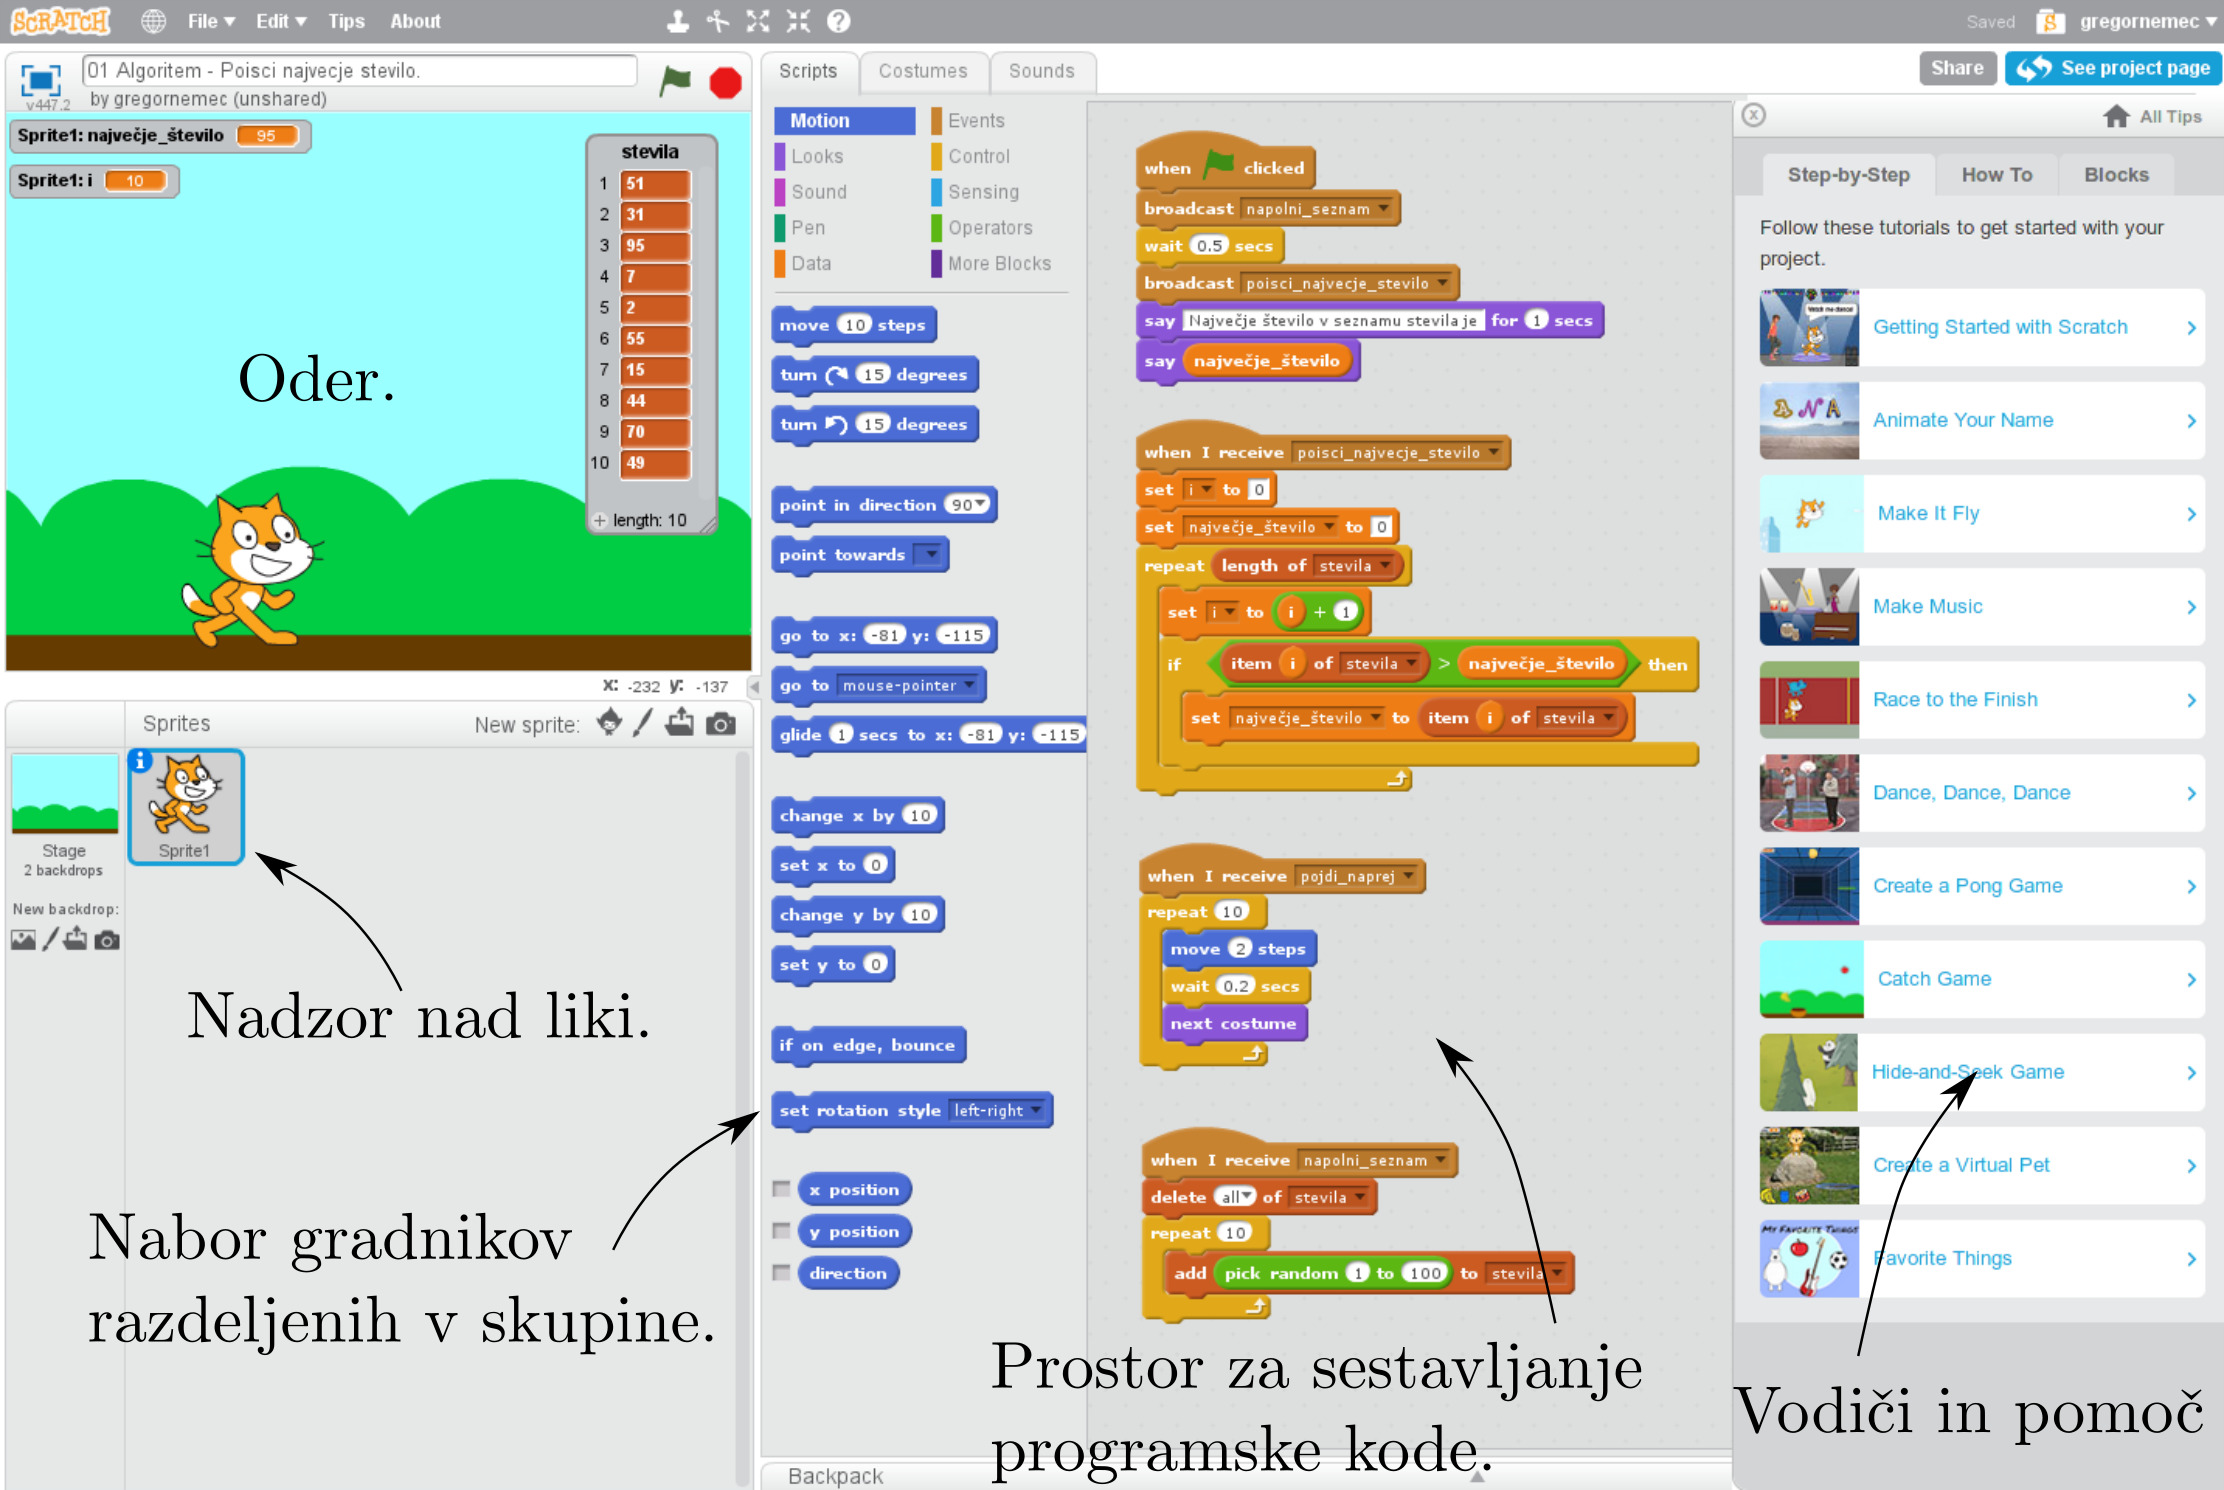
\includegraphics [width=0.90\linewidth, keepaspectratio =
   1] {./images/sc_web/scratch_orodje-v021.jpg}
   \caption{Zaslonska slika
     \emph{\href{https://scratch.mit.edu/}{Scratch}}
     \cite{web:scratch}.}
    \label{fig:web:scratch:orodje}
\end{figure}

\textbf{Vodiče} v Scratchu najdemo na desnem robu (slika+
\ref{fig:web:scratch:orodje}). Vodiči so sestavljeni tako, da
uporabnika postopoma vodijo skozi gradnjo programa. S tem je
zagotovljena \textbf{postopnost}. Posamezen korak v vodiču je
sestavljen iz besedila in animiranega poteka dela.

\subsubsection{Deljenje in raziskovanje projektov}
\label{sec:deljenje_vsebin}

Vsak uporabnik, ki se registrira na spletnem portalu ima dostop do
svojega profila. Na svoji strani se samodejno shranjujejo projekti, ki
smo jih izdelovali in jih od tu lahko ponovno naložimo za
urejanje. Vse projekte lahko delimo z drugimi. Vsak projekt ima svojo
pod stran na kateri določamo nastavitve za \emph{deljenje} (slika
\ref{fig:web:scratch:deljenje}). Na strani lahko dodamo \emph{navodila
  za program} in \emph{zapiske in zasluge}, prav tako določamo, če
želimo projekt deliti ali ne.

\begin{figure}[h!]
  \centering
    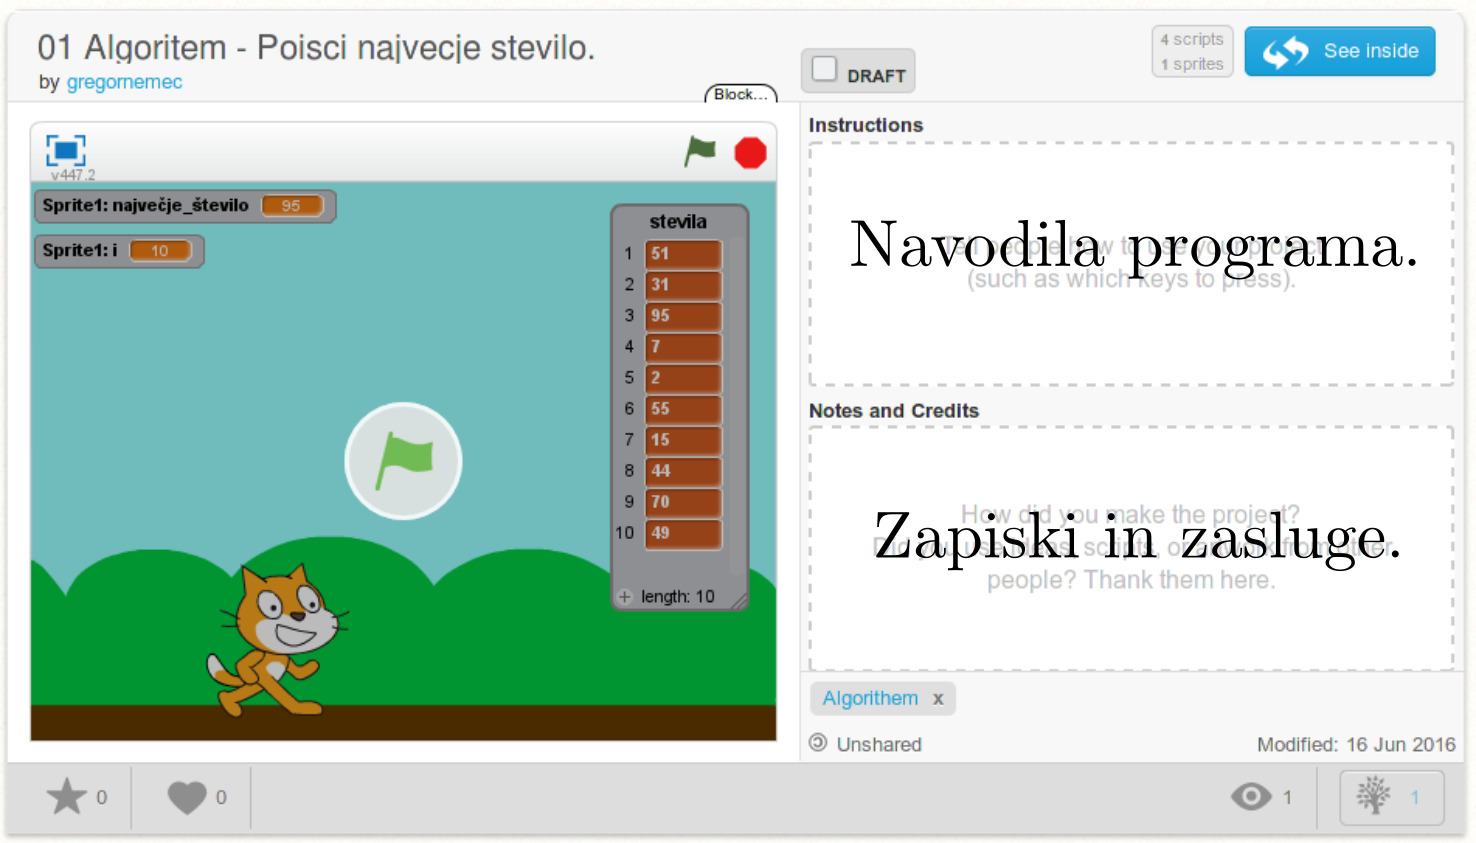
\includegraphics [width=0.50\linewidth, keepaspectratio =
   1] {./images/sc_web/scratch_deljenje-v01o.jpg}
   \caption{Pod stran za deljenje projekta na
     \emph{\href{https://scratch.mit.edu/}{Scratch}}
     \cite{web:scratch}.}
    \label{fig:web:scratch:deljenje}
\end{figure}

Če je omogočeno da lahko delimo vsebine je na spletnem portalu tudi
dobro poskrbljeno za \textbf{raziskovanje projektov} drugih
uporabnikov. Pod zavihkom \emph{razišči (ang. Explor)} najdemo
številne projekte, ki so razporejeni v kategorije. Tu lahko črpamo
številne ideje in si najljubše projekte shranimo tudi na svojem
profilu.

\subsubsection{Povzetek}
\label{sec:scratch_povzetek}

\textbf{Učni načrt} v slovenski osnovni šoli ne obveznega izbirnega
predmeta \textbf{Računalništvo} je prilagojen prav za uporabo
Scratcha, kot je razvidno iz ciljev. Čeprav z dobro pripravljenimi
vodiči spoznavamo tudi na primer vejitve, si učitelj mora pripraviti
in prilagoditi vsebino za uresničevanja učnega načrta sam. Kot smo že
lahko ugotovili, na spletu in na sploh ne zmanjka literature in idej,
ki učitelju pomagajo pri uresničevanju učnega načrta s Scratchem. Tudi
na spletni strani Scratcha lahko črpamo številne ideje iz projektov
drugih uporabnikov.

Za slabost spletne različice štejemo, da je narejen z zaprto
tehnologijo \textbf{Adobe Flash}, kar pomeni, da si uporabnik mora
naložiti vtičnik Flash za spletni brskalnik. Vtičnik Flash uradno
podpira le nekatere komercialne operacijske sisteme in njegovo vlogo
zamenjuje vedno boljše zmožnosti samih spletnih brskalnikov z
tehnologijo \textbf{HTML5 + CSS + JS}.

\begin{osebnabox}[label={osebna:scratch}]{Scratch | \url{https://scratch.mit.edu}}
    \begin{tabular}{
  p{0.30\linewidth-2\tabcolsep} |
  p{0.70\linewidth-2\tabcolsep}  }
  \textbf{Vrsta vsebine} & Spletna aplikacija za prog. \\
      \hline
  \textbf{Jezik spletne strani} & Scratch: angleščina: da, slovenščina: da,
                                  drugi: da. Spletni portal:
                                  angleščina: da, drugi: ne\\
      \hline
  \textbf{Ponujena znanja} & Vodiči za spoznavanje uporabe Scratch in pomoč \\
      \hline
 \textbf{Programski jeziki} & Scratch \\
      \hline
  \textbf{Težavnostna stopnja} & Osnovna šola \\
      \hline
   \textbf{Upoštevanje načel} & Problemski pristop: ne,
                                sistematičnost: ne, postopnost: da (Vodič). \\
      \hline
  \textbf{Dosežki/Gamification} & Ne. \\
      \hline
  \textbf{Dodajanje lastnih vsebin} & Da, vendar v smislu ustvarjanja
                                      lastnih projektov in ne
                                      celovitih vadnic. \\
      \hline
  \textbf{Upravljanje razreda} & Ne. \\
      \hline
  \textbf{Dostop vsebin} & Brezplačen. \\
\end{tabular}
\end{osebnabox}

\subsection{Repl.it}
\label{sec:repl.it}

\textbf{\emph{\href{https://repl.it/}{Repl.it}}} \cite{web:replIT} je še ena
\textbf{spletna aplikacija za programiranje}. Podjetje, ki spletno
stran ustvarja je tržno osredotočeno na ponujanje \textbf{aplikacijski
  programski vmesnik - APV} ali (\emph{ang. application programming
  interface - \textbf{API}}). Njihov APV uporabljajo številni spletni
portali kot je na primer
\emph{\href{freecodecamp}{https://www.freecodecamp.com}}
\cite{web:freecodecamp} in nekateri drugi plačljivi spletni
portali. Na svoji strani ponujajo prost dostop do spletne aplikacije
za programiranje (slika \ref{fig:web:replIT}).

\begin{figure}[h!]
  \centering
    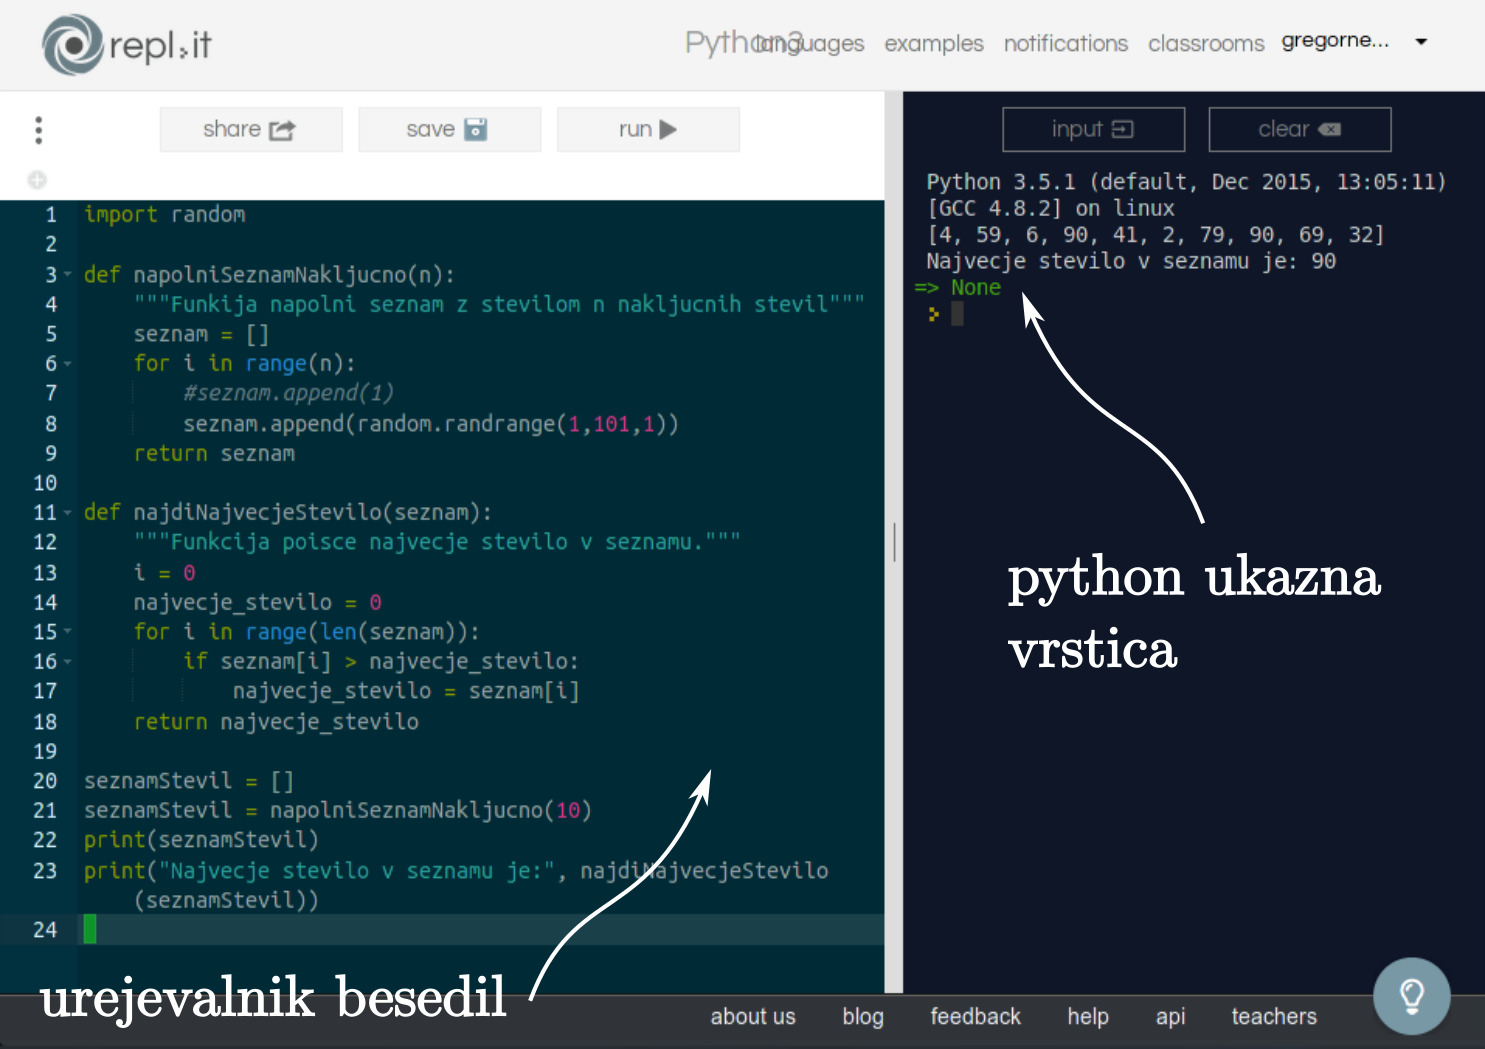
\includegraphics [width=0.65\linewidth, keepaspectratio =
   1] {./images/sc_web/replIT_main-v01.jpg}
   \caption{Zaslonska slika spletne aplikacije za programiranje
     \emph{\href{https://repl.it/}{repl.it}} \cite{web:replIT}.}
    \label{fig:web:replIT}
\end{figure}

Aplikacija ponuja številne programske jezike kot je \textbf{Python3,
  Ruby, JavaScript, HTML, CSS, C\#, JAVA} in še mnoge druge. Vsako nova
pojava spletne aplikacije predstavlja novo sejo. Po registraciji na
spletnem portalu lahko shranjujemo posamezne seje. Posamezno sejo
lahko \textbf{tudi delimo} preko spletne povezave. \textbf{Urejevalnik
  besedil} omogoča barvanje rezerviranih besed programske kode in ima napredno
\textbf{možnost ponujanja predlogov} za samo dokončevanje izpisa
rezerviranih besed in funkcij programskega jezika.

\subsubsection{Ustvarjanje razredov in nalog}
\label{sec:ustvarjanje_raz_nalog}

Spletni portal skorja, da ni vreden omembe z \textbf{vsebinskega
  vidika} tudi kot spletna aplikacija me predstavlja nekih posebnih
funkcij, ki jih nebi imele tudi nekatere druge spletne aplikacije. Ima
pa spletni portal veliko zmožnost, saj omogoča \textbf{ustvarjanje
  razredov}. Mentor lahko ustvarja razred in v njega povabi dijake ter
samodejno dodaja oz. \textbf{ustvarja lastne naloge}
oz. \textbf{vadnice} (slika \ref{fig:web:replIT:assigment}). Dijake v
razred povabi z dodajanjem email-ov v seznam. Dijakom ni potrebna
registracija. S povezavo, ki so jo dobili na email se prijavijo v
razred. Mentor v načinu ustvarjanja naloge, doda lastna navodila in
začetno programsko kodo. V naslednjem koraku se mentor lahko odloči
ali bo pravilnost naloge preverjal sam ali po dodal avtomatski
preizkus programske kode. V avtomatskem načinu mora podati primer
vhodnih podatkov in rezultat izhoda.

V razredu imajo dijaki vpogled v seznam nalog. Naloge se dijakom
prikazane z navodili. Dijaki rešujejo nalogo in ko so zadovoljni s
svojo rešitvijo, nalogo oddajo. Mentorju se status naloge pri dijaku
spremeni na \emph{oddano} in sedaj mentor nalogo lahko pregleda, poda
komentar in jo označi kot \emph{opravljeno} ali jih s sporočilom tudi
\emph{zavrne}.

\begin{figure}[h!]
  \centering
    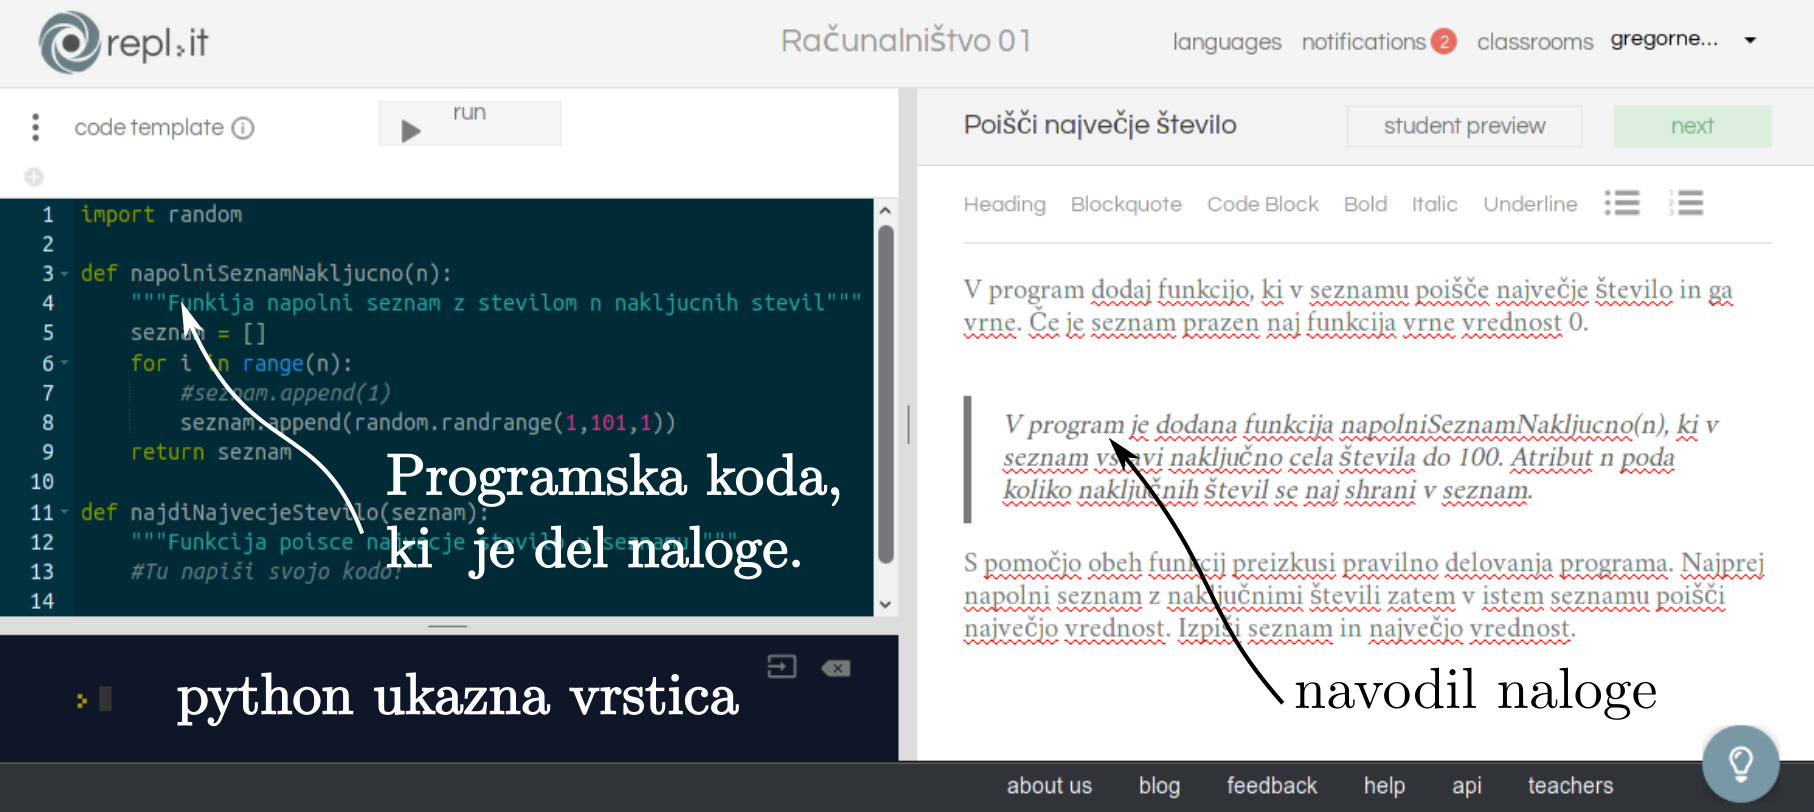
\includegraphics [width=0.65\linewidth, keepaspectratio =
   1] {./images/sc_web/replIT_assigment-v01.jpg}
   \caption{Zaslonska slika pogleda mentorja v načinu priprave naloge
     \cite{web:replIT}.}
    \label{fig:web:replIT:assigment}
\end{figure}

\subsubsection{Povzetek}
\label{sec:povzetek:replIT}

Spletna aplikacij za programiranje, ponuja mentorjem računalniških
vsebin osnovno orodje za ustvarjanje razredov in nalog ter
komunikacijo z dijaki. Pri tem uporablja osnovne zmožnosti brez
pretirane kompleksnosti. Sam spletni portal ne ponuja nobene vsebine,
kar je sovje vrstna prednost, saj lahko mentor prilagodi naloge učnemu
načrtu in to v svojem jeziku.

\begin{osebnabox}[label={osebna:replIT}]{Repl.it | \url{https://repl.it/}}
    \begin{tabular}{
  p{0.30\linewidth-2\tabcolsep} |
  p{0.70\linewidth-2\tabcolsep}  }
  \textbf{Vrsta vsebine} & Spletna aplikacija za prog. \\
      \hline
  \textbf{Jezik spletne strani} & angleščina: da, slovenščina: ne,
                                  drugi: ne. \\
      \hline
  \textbf{Ponujena znanja} & Ne ponuja nobene vsebine\\
      \hline
 \textbf{Programski jeziki} & Python3,
  Ruby, JavaScript, HTML, CSS, C\#, JAVA in drugi\\
      \hline
  \textbf{Težavnostna stopnja} & Srednja šola.\\
      \hline
   \textbf{Upoštevanje načel} & Problemski pristop: ne,
                                sistematičnost: ne, postopnost: ne (Vodič). \\
      \hline
  \textbf{Dosežki/Gamification} & Ne. \\
      \hline
  \textbf{Dodajanje lastnih vsebin} & Da. Ustvarjanje razreda in nalog
                                      ter komunikacija z dijaki. \\
      \hline
  \textbf{Upravljanje razreda} & Da. \\
      \hline
  \textbf{Dostop vsebin} & Brezplačen. \\

\end{tabular}
\end{osebnabox}

\subsection{Tutorialspoint}
\label{sec:tutorials_point}

\emph{\href{http://www.tutorialspoint.com/}{Tutorials point}}
\cite{web:tutorialspoint} je eden izmed velikih portalov, ki ponujajo
obsežne in zahtevne vodiče tehničnih in ne tehničnih vsebin. Na
spletu je vodičev veliko, tega smo izpostavili iz razloga, ker ponuja
ogromno \textbf{vsebin programiranja in računalniške znanosti}, vsi
primeri v vodičih imajo \textbf{možnost preizkusa} in razvito imajo
lastno \textbf{spletno aplikacijo za programiranje}, ki ima veliko
zmožnosti, nekatere značilne za namizne \textbf{IDE}.

Spletni portal ponuja knjižnico vodičev (\ref{fig:web:tutpoint:lib})
različnih vsebinskih sklopov. Z slike je razvidno, da je zares
obsežna.

\begin{figure}[h!]
  \centering
    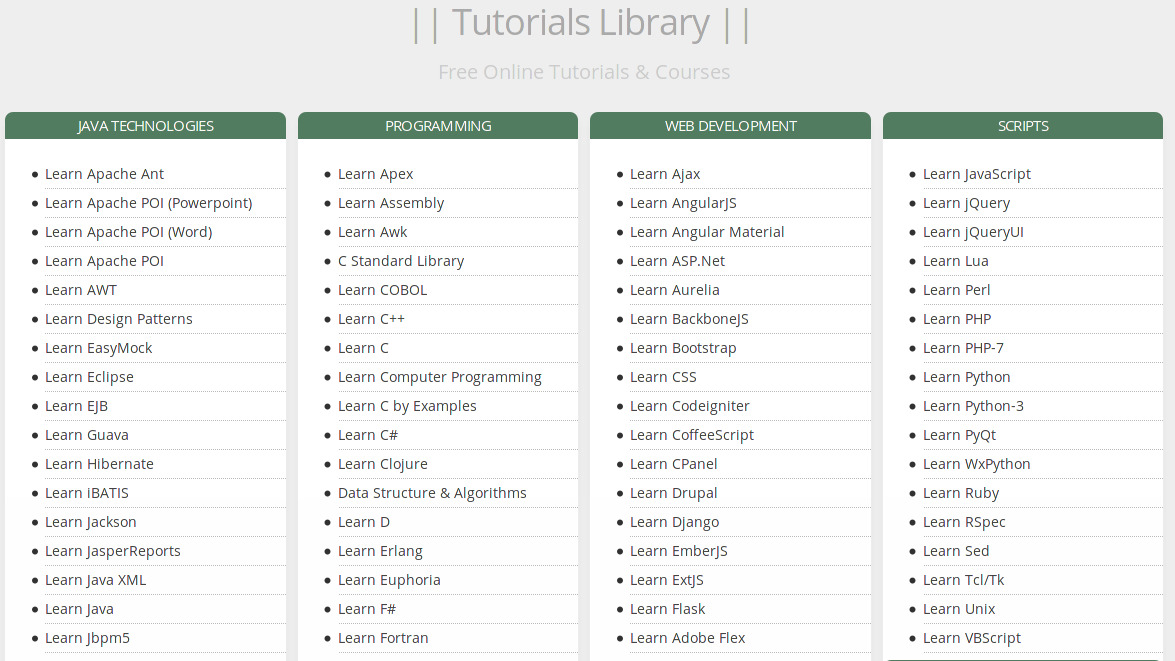
\includegraphics [width=0.65\linewidth, keepaspectratio =
   1] {./images/sc_web/tutpoint_lib-v01.jpg}
   \caption{Del seznama oz knjižnica vodičev, ki ga ponuja spletna
     stran \emph{\href{http://www.tutorialspoint.com/}{Tutorials
         point}} \cite{web:tutorialspoint}.}
    \label{fig:web:tutpoint:lib}
\end{figure}

Vsebinsko si smo pregledali vodič za \textbf{Python3} (slika
\ref{fig:web:tutpoint:tut01}). Vodiči so oblikovani tako, da na desni
strani najdemo kazalo vsebine, v sredinskem delu je razložena snov z
primeri.

%Dodaj besedilo v sliko.
\begin{figure}[h!]
  \centering
    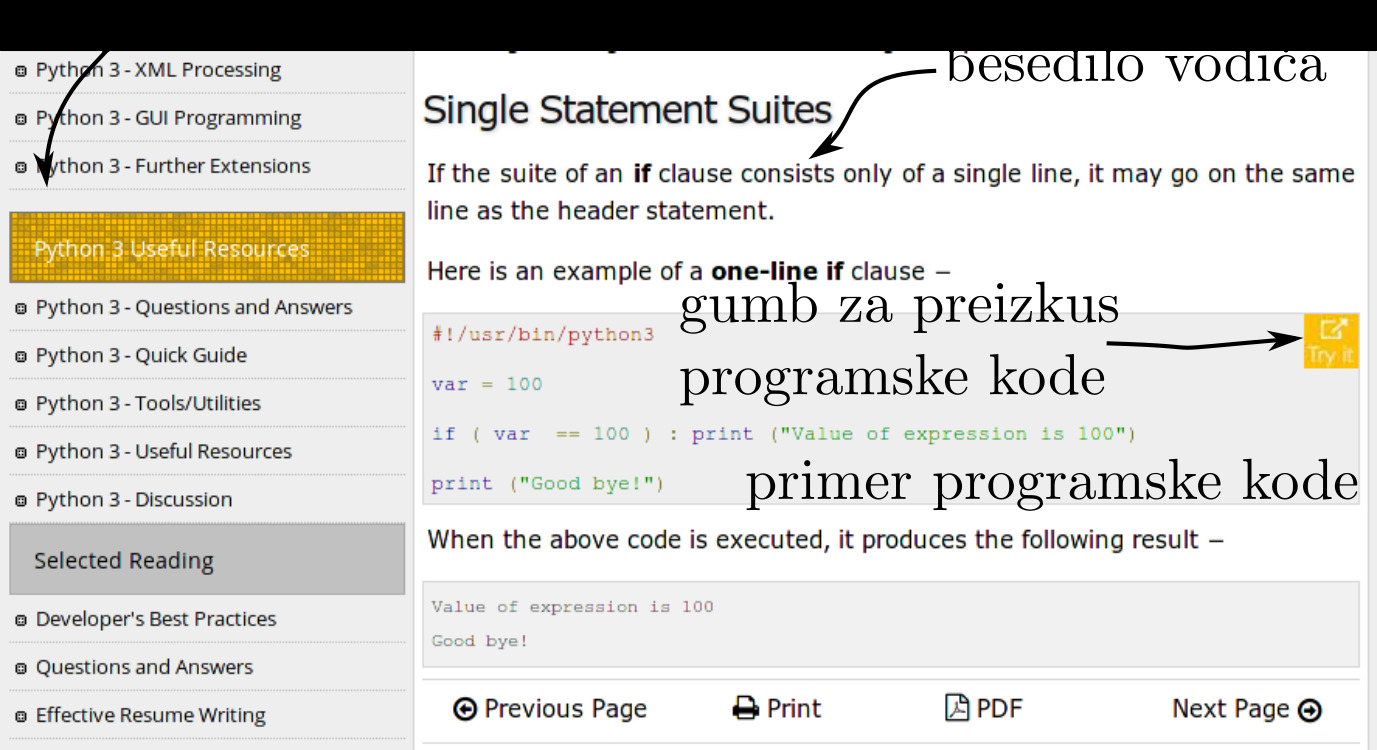
\includegraphics [width=0.65\linewidth, keepaspectratio =
   1] {./images/sc_web/tutpoint_tutP3-v01.jpg}
   \caption{Zaslonski izrez vodiča za Python3. S like je razvidno
     kazalo in gumb za \textbf{Preizkus!} \cite{web:tutorialspoint}.}
    \label{fig:web:tutpoint:tut01}
\end{figure}

Nekatere od primerov lahko tudi preizkusimo, z klikom na gumb
\textbf{Preizkusi (\emph{ang. Try it})}, se nam na isti strani odpre
podokno (slika \ref{fig:web:tutpoint:tut02}). Kodo v urejevalniku
lahko spreminjamo in ponovno zaženemo.

%Dodaj besedilo v sliko.
\begin{figure}[h!]
  \centering
    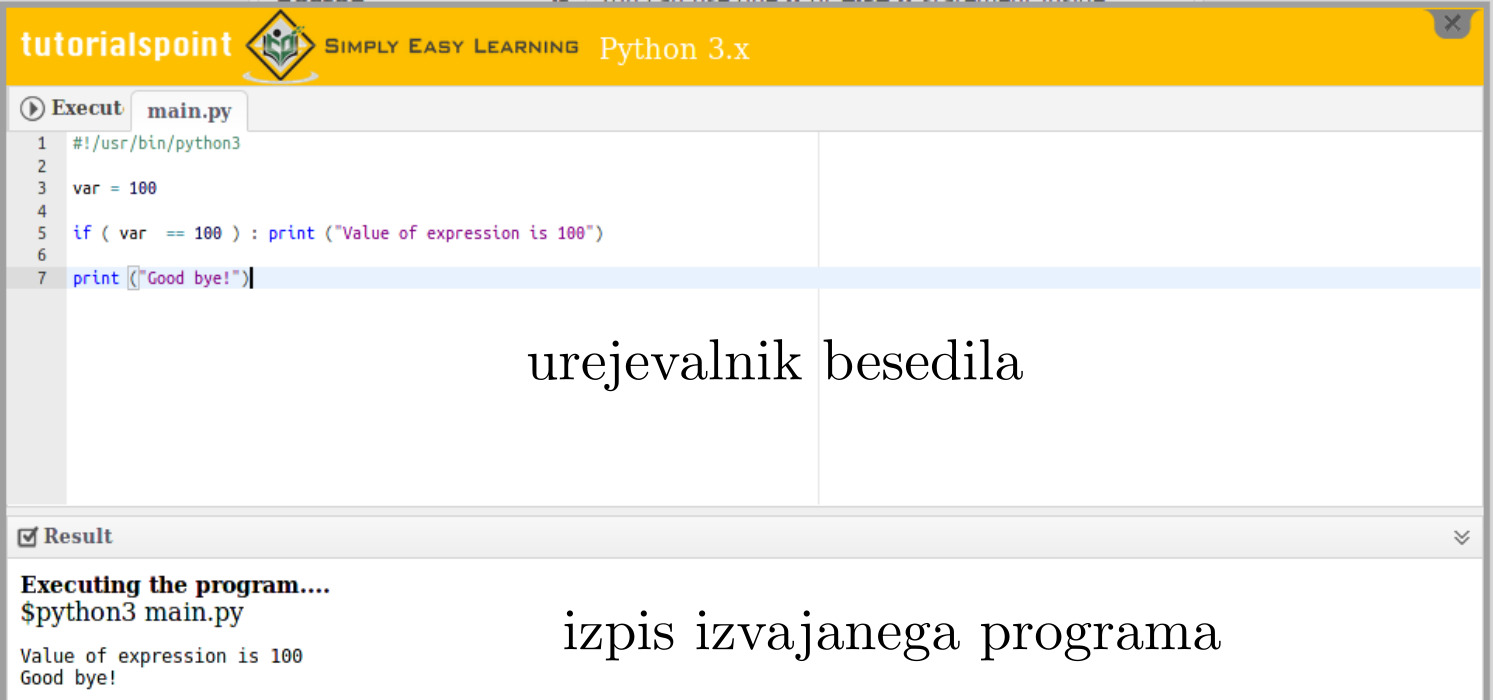
\includegraphics [width=0.65\linewidth, keepaspectratio =
   1] {./images/sc_web/tutpoint_tutP3-v02.jpg}
   \caption{Pod okno za preizkus primera programske kode
     \cite{web:tutorialspoint}.}
    \label{fig:web:tutpoint:tut02}
\end{figure}

\subsubsection{Coding ground}
\label{sec:coding_ground}

Kot smo že omenili spletni portal kot orodje ponuja lastno spletno
aplikacijo za programiranje. Spletna aplikacija se imenuje
\emph{\href{http://www.tutorialspoint.com/codingground.htm}{Codingground}}
\cite{web:tutorialspoint:codingground}. Na uvodni strani orodja (slika
\ref{fig:web:tutpoint:cg-pl}) smo odkrili, številnost ponujenih
\textbf{programskih jezikov}, ki sovpadajo s številnimi vodiči, ki jih
ponuja spletni portal.

\begin{figure}[h!]
  \centering
    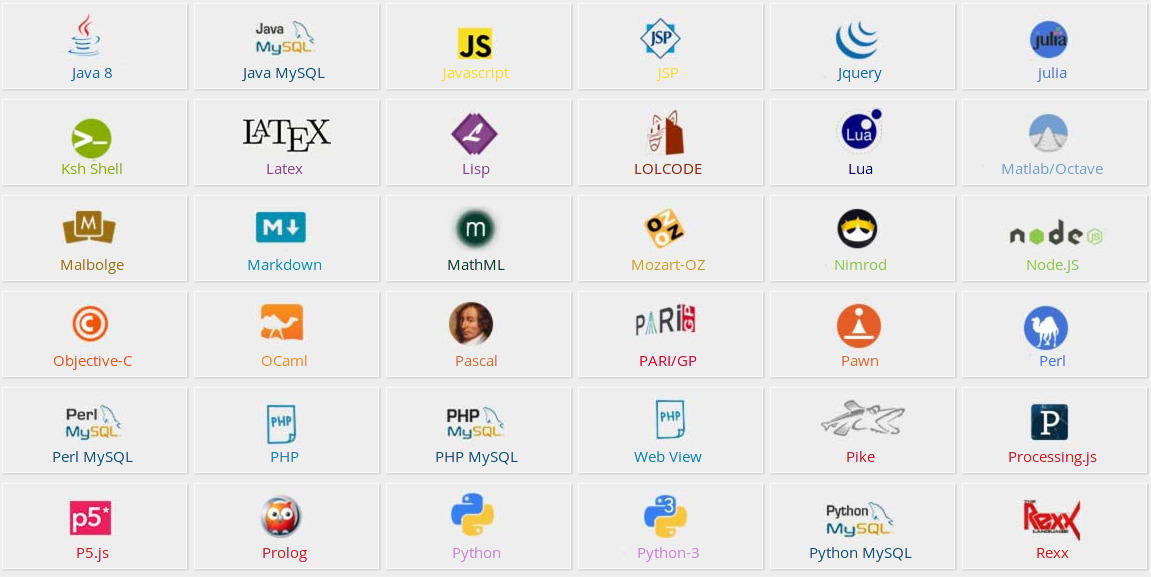
\includegraphics [width=0.65\linewidth, keepaspectratio =
   1] {./images/sc_web/tutpoint_cg-pl-v01.jpg}
   \caption{Del seznama različnih programskih jezikov katere lahko
     uporabljamo z spletno aplikacijo za programiranje
     \emph{\href{http://www.tutorialspoint.com/codingground.htm}{Codingground}}
     \cite{web:tutorialspoint:codingground}.}
    \label{fig:web:tutpoint:cg-pl}
\end{figure}

Razporeditev spletne aplikacije (slika \ref{fig:web:tutpoint:cg}) je
taka, da na levem robu imamo seznam datotek v korenskem imeniku, v
sredinskem delu je urejevalnik besedil, nad urejevalnikom najdemo
menijsko vrstico in na dnu strani je \textbf{ukazna vrstica}, v kateri
lahko zaganjamo napisano programsko kodo. V njej se izpisujejo tudi
povratne informacije tolmača in izhod programske
kode. \textbf{Urejevalnik besedil} besedil omogoča barvanje kode
rezerviranih besed in nastavljanje barvne sheme
urejevalnika. Urejevalnik omogoča še samodejno zamikanje programske
kode, ko je to potrebno. \textbf{Shranjevanje in uvažanje projektov v
  oblak}, lahko smatramo kot eno izmed večjih zmožnosti te spletne
aplikacije. \emph{\href{http://www.tutorialspoint.com/codingground.htm}{Codingground}}
lahko nastavimo, da se poveže s oblačnimi shrambami kot so
\textbf{Dropbox, Google Drive, Onedrive} in s sistemom za objavljanje,
upravljanje verzij in kolaboracijo \textbf{Git}. Seveda lahko projekt
naložimo neposredno z računalnika in ga seveda tja tudi
shranimo. Prednost oblačnega shranjevanja je ta, da na programiramo
lahko od koder koli in z katerim orodjem želimo. če je to spletna
aplikacija ali namizna. Spletna aplikacija omogoča tudi upravljanje z
datotekami. Lahko ustvarimo, preimenujemo in brišemo datoteke ali
imenike. To lahko počnemo z \textbf{menija (\emph{file}) ali ukazne
  vrstice}. Vsak projekt lahko delimo preko neposredne kratke
\textbf{url povezave}, kot smo to že videli pri drugih spletnih
portalih.

\begin{figure}[h!]
  \centering
    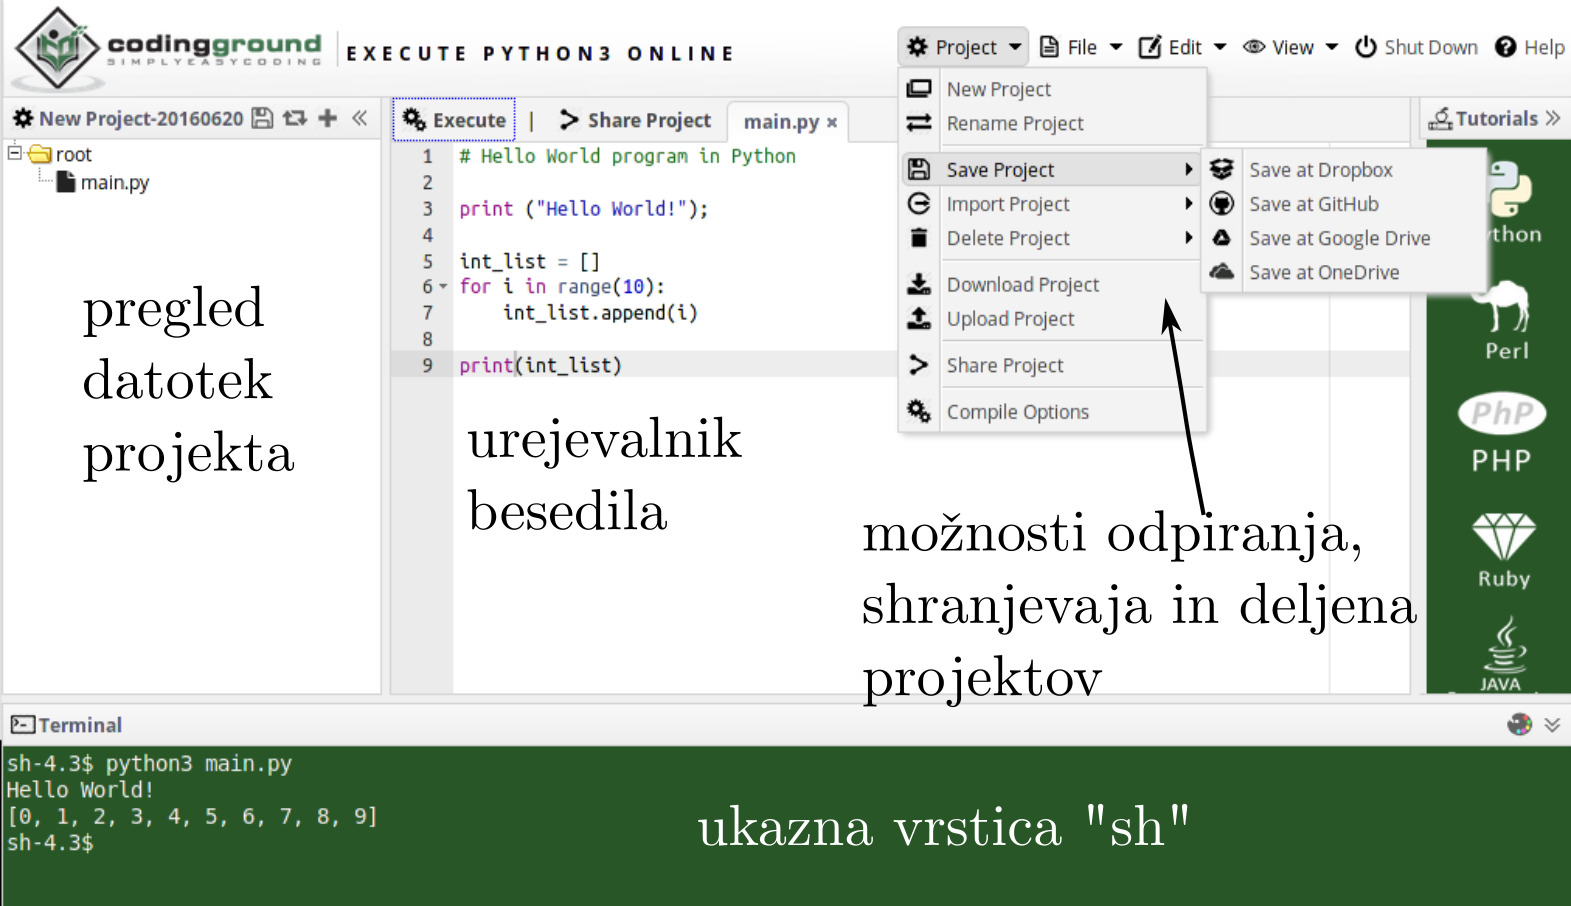
\includegraphics [width=0.65\linewidth, keepaspectratio =
   1] {./images/sc_web/tutpoint_cg-v01.jpg}
   \caption{Spletna aplikacija za programiranje -
     \emph{\href{http://www.tutorialspoint.com/codingground.htm}{Codingground}}
     \cite{web:tutorialspoint:codingground}.}
    \label{fig:web:tutpoint:cg}
\end{figure}

\subsubsection{Povzetek}
\label{sec:povzetek_tutpoint}

Vsebina vodičev je zelo tehnična in deluje kot okrnjen povzetek uradne
reference za določen programski jezik. Kot taka je predvsem primerna
za programerje začetnike, ki se želijo poučiti o določenem programskem
jeziku, vendar že poznajo osnovne koncepte programiranja. Velik plus
je vsekakor preizkus programske kode. Vodiče lahko priporočimo kot
skrajšano verzijo reference programskemu jeziku.

S pravo nastavitvijo, spletna aplikacija omogoča, da dijaki imajo
programsko kodo in snov, ki jo v nekem trenutku predelujejo povsod na
voljo. S pomočjo shranjevanja in deljenja projektov lahko mentor
uporabi spletno aplikacijo kot glavno orodje za učenje računalništva
in programskega jezika. Mentor mora pripraviti sistem za izmenjavo
navodil, programske kode, in rešitev dijakov. To lahko stori uporabo
kratkih url povezav. Urejevalnik besedil bi lahko ponujal kakšno
zmožnost več kot jo, vendar zadosti osnovnim potrebam pisanja
programske kode.


\begin{osebnabox}[label={osebna:tutorails point}]{Tutorialspoint |
    \url{http://www.tutorialspoint.com/}}
    \begin{tabular}{
  p{0.30\linewidth-2\tabcolsep} |
  p{0.70\linewidth-2\tabcolsep}  }
  \textbf{Vrsta vsebine} & Osnova kombinirana vsebina: vodič in
                           preizkus programske kode. Posebej spletna
                           aplikacija za učenje programiranja:
                           Codingground \\
      \hline
  \textbf{Jezik spletne strani} & angleščina: da, slovenščina: ne,
                                  drugi: ne. \\
      \hline
  \textbf{Ponujena znanja} & Znanja prog. Jezikov + druge
                             vsebine. Vodiči s številnih področij. \\
      \hline
 \textbf{Programski jeziki} & Velika knjižnica prog. Jezikov \\
      \hline
  \textbf{Težavnostna stopnja} & Srednja šola.\\
      \hline
   \textbf{Upoštevanje načel} & Problemski pristop: ne,
                                sistematičnost: ne, postopnost: da (Vodič). \\
      \hline
  \textbf{Dosežki/Gamification} & Ne. \\
      \hline
  \textbf{Dodajanje lastnih vsebin} & Da. Ustvarjanje podporne
                                      programske kode v spletni
                                      aplikaciji za prog., vendar brez
                                      navodil in deljenje vsebine.  \\
      \hline
  \textbf{Upravljanje razreda} & Na. \\
      \hline
  \textbf{Dostop vsebin} & Brezplačen. \\

\end{tabular}
\end{osebnabox}

\subsection{Thimble}
\label{sec:thimble}

%Vodič je lahko vodnik, spremeni!?

\emph{\href{https://thimble.mozilla.org/sl/}{Thimble}}
\cite{web:thimble} je spletni portal, ki ga gosti podjetje
\textbf{mozilla}, katero izdaja spletni brskalnik
\textbf{Firefox}. Spletni portal je namenjen učenju spletnih
tehnologij \textbf{HTML, CSS} in \textbf{Java Script}. Pripravljenih
je šest spletnih vsebin, ki jih lahko odpremo v projektu in jih
preurejamo. Največja prednost spletnega portala je spletna aplikacija
oz. orodje v katerem urejamo projekte (slika
\ref{fig:web:thimble:webapp}).

\begin{figure}[h!]
  \centering
    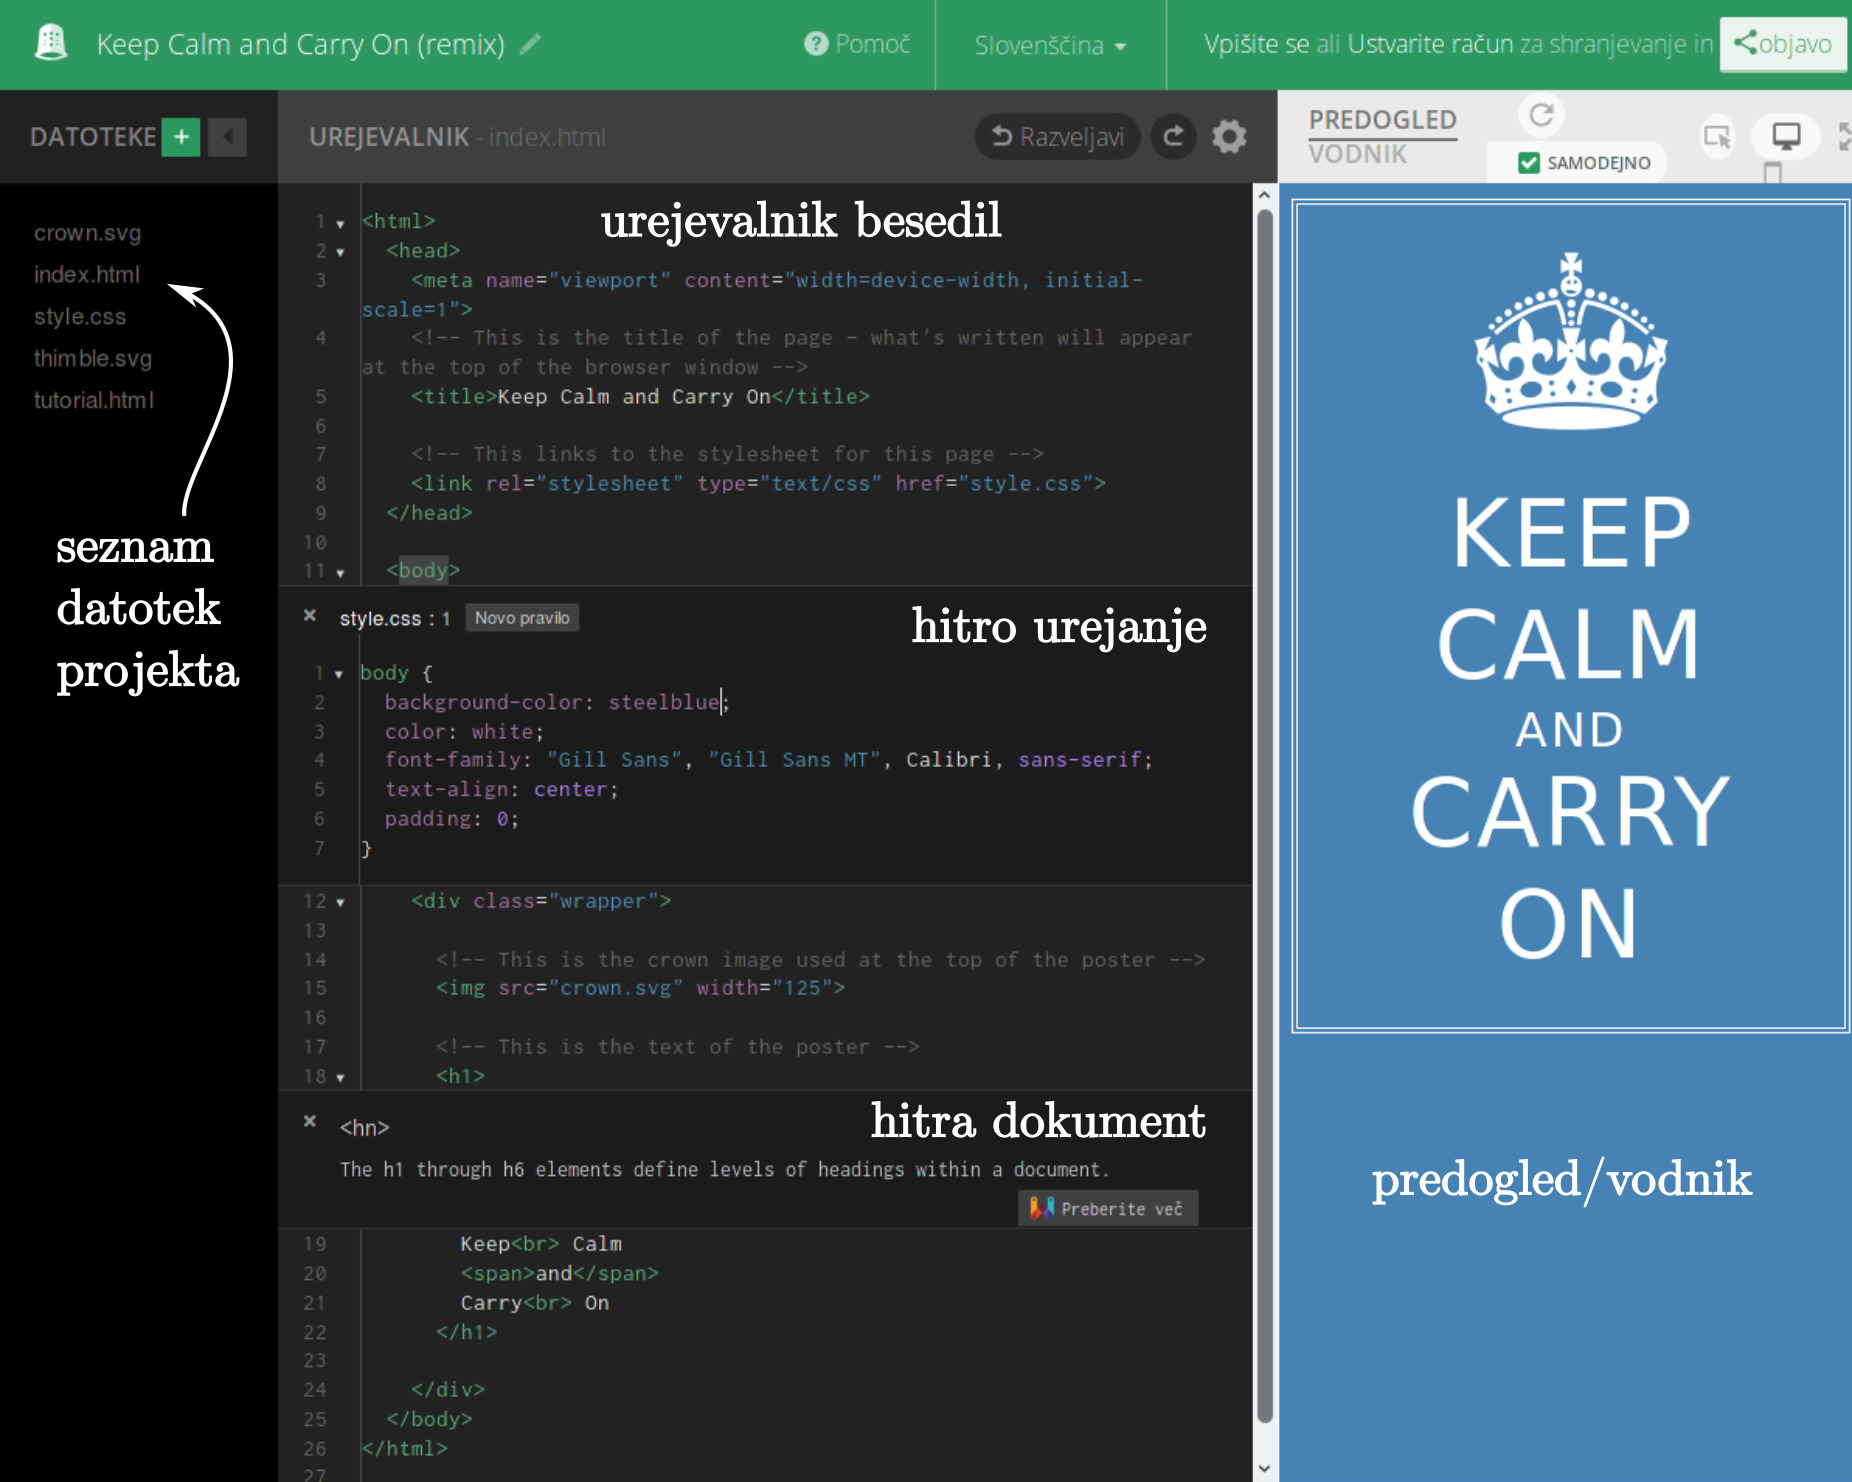
\includegraphics [width=1\linewidth, keepaspectratio =
   1] {./images/sc_web/thimble_saup-v02.jpg}
   \caption{Urejanje projekta na strani
     \emph{\href{https://thimble.mozilla.org/sl/}{Thimble}}
     \cite{web:thimble}.}
   \label{fig:web:thimble:webapp}
 \end{figure}

 Na desni strani spletne aplikacije imamo \textbf{seznam dokumentov},
 ki sestavljajo projekt. V projekt lahko dodajamo lastne dokumente.
 \textbf{Urejevalnik besedil} barva značke html in css jezika, prav
 tako upošteva barvanje besedila v primeru programskega jezika
 JavaScript. Urejevalnik ima dve priročni zmožnosti, kot je
 \emph{hitri dokument} in \emph{hitro urejanje}. Hitri dokument je
 takojšnja pomoč, ki se sproži ob pritisku kombinacije \texttt{Alt +
   K} na mestu kjer je značka za katero želimo dodatno razlago. Hitro
 ureja na mestu, kjer smo postavljeni v besedilu z pritiskom
 kombinacije tipk \texttt{Alt+E} odpre pod urejevalnik z \emph{css}
 razredom, ki oblikuje značko dela html dokumenta. Funkcija hitro
 urejanje v \emph{css} dokumentu, ko smo postavljeni na barvo, pomeni
 barve s barvne palete.

 Vse spremembe, ki jih naredimo v urejevalniku se v živo in samodejno
 posodobijo v \textbf{oknu predogleda}, ki se nahaja na levem delu. Na
 tem mestu najdemo tudi vodnika.  Uvodna spletna stran in uporabniški
 vmesnik sta preveden v \textbf{slovenščino}. Žal pa vodniki, ki so
 del pripravljeni na spletni strani niso prevedeni v slovenščino.

 Če na spletni strani opravimo registracijo in se prijavimo, se nam
 spremembe na projektu shranjujejo samodejno. Projekt lahko
 preimenujemo in ga delimo z drugimi preko spletne povezave. Tisti, ki
 naš projekt odpre ga spreminja kot lastnega in se sprememba v našem
 ne pozna. Ustvarjamo lahko tudi nove projekte, katerim dodajamo
 \texttt{html, css, js} datoteke. Dodamo lahko tudi, datoteko vodiča,
 ki jo lahko poljubno spreminjamo.
 
\subsubsection{Povzetek}
\label{sec:povzetek_thimble}

Spletni portal lahko uporabljamo na vseh stopnjah. Primeren je še
posebej za uporabo v osnovni šoli pri izbirnem predmetu
\textbf{Računalniška omrežja}, saj omogoča enostaven in učinkovit
urejevalnik besedil. Učitelj se registrira in pripravi oz prilagodi
obstoječi projekt za pouk. Učencem deli povezavo. Učencem se ni
potrebno registrirati in kljub temu lahko urejajo dokument. Učenci,
svoje dokončane projekte delijo kot končen izdelek s povezavo nazaj
učitelju. Na podoben način se lahko spletni portal uporablja tudi v
srednji šoli.

\begin{osebnabox}[label={osebna:thimble}]{Thimble |
    \url{https://thimble.mozilla.org}}
    \begin{tabular}{
  p{0.30\linewidth-2\tabcolsep} |
  p{0.70\linewidth-2\tabcolsep}  }
  \textbf{Vrsta vsebine} & Napredna kombinirana vsebina: Vadnica
                           (Vodnik + spletna aplikacija za
                           programiranje).   \\
      \hline
  \textbf{Jezik spletne strani} & angleščina: da, slovenščina:
                                  aplikacij, da; vodnik, ne. 
                                  drugi: da. \\
      \hline
  \textbf{Ponujena znanja} & Znanje programskih jezikov, uporaba
                             spletna in spletnih vsebin. \\
      \hline
 \textbf{Programski jeziki} & HTML, CSS, JavaScript. \\
      \hline
  \textbf{Težavnostna stopnja} & Osnovno šolo (3. triado) in srednjo
                                 šolo. \\
      \hline
   \textbf{Upoštevanje načel} & Problemski pristop: da,
                                sistematičnost: ne, postopnost: ne \\
      \hline
  \textbf{Dosežki/Gamification} & Ne. \\
      \hline
  \textbf{Dodajanje lastnih vsebin} & Da. Možno je ustvarjanje lastnih
                                      vadnic, ki jih lahko delimo
                                      naprej.  \\
      \hline
  \textbf{Upravljanje razreda} & Na. \\
      \hline
  \textbf{Dostop vsebin} & Brezplačen. \\

\end{tabular}
\end{osebnabox}


\subsection{Code combat}
\label{sec:code_battle}

Spletni portal \emph{\href{https://codecombat.com/}{Code combat}}
\cite{web:codecombat} je mešanica med igranjem igre in pisanjem
programske kode. V predstavitvi spletne strani pravijo naslednje,
\emph{``Če se želiš naučiti programirati, moraš napisati veliko
  programske kode''} in poudarjajo, da oni poskrbijo da pri tem
početju ostane zabava v ospredju \cite{web:codecombat:about}. Spletna
stran ponuja tri načine registracije, ustvarite lahko
\textbf{navaden}, \textbf{učiteljski} ali \textbf{učencev}, račun. V
pregledu strani smo uporabili prijavo z navadnim računom, v
nadaljevanju smo prav tako povzeli posebnosti ostalih dveh računov.

Po registracij in prijavi v račun si izberemo \textbf{lik in
  programski jezik} s katerim bomo igrali (slika
\ref{fig:web:cc:hero}). Spletna igra ponuja štiri programske jezike
\textbf{Python, JavaScript, CoffeScript, LUA}. 

\begin{figure}[h!]
  \centering
    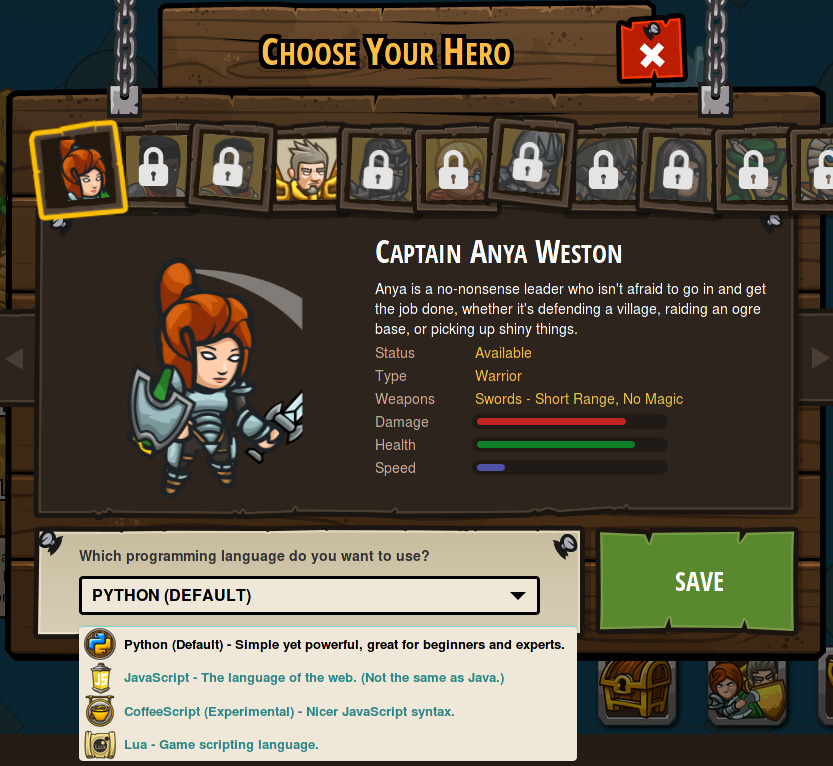
\includegraphics [width=0.45\linewidth, keepaspectratio =
   1] {./images/sc_web/cc_hero-lang-v01.jpg}
   \caption{Izbira junaka in programskega jezika \cite{web:codecombat}.}
   \label{fig:web:cc:hero}
 \end{figure}


 Po izbiri junaka preidemo na izbor \textbf{zemljevidov} (slika
 \ref{fig:web:cc:zemljevid}). Izberemo lahko samo zemljevid, ki je
 odklenjen. Druge zemljevide odklenemo tako, da rešimo vse naloge v
 njem. Posamezen zemljevid predstavlja cilje posameznih programskih
 konceptov, ki se jih uporabnik nauči, ko predela vse naloge.

\begin{figure}[h!]
  \centering
    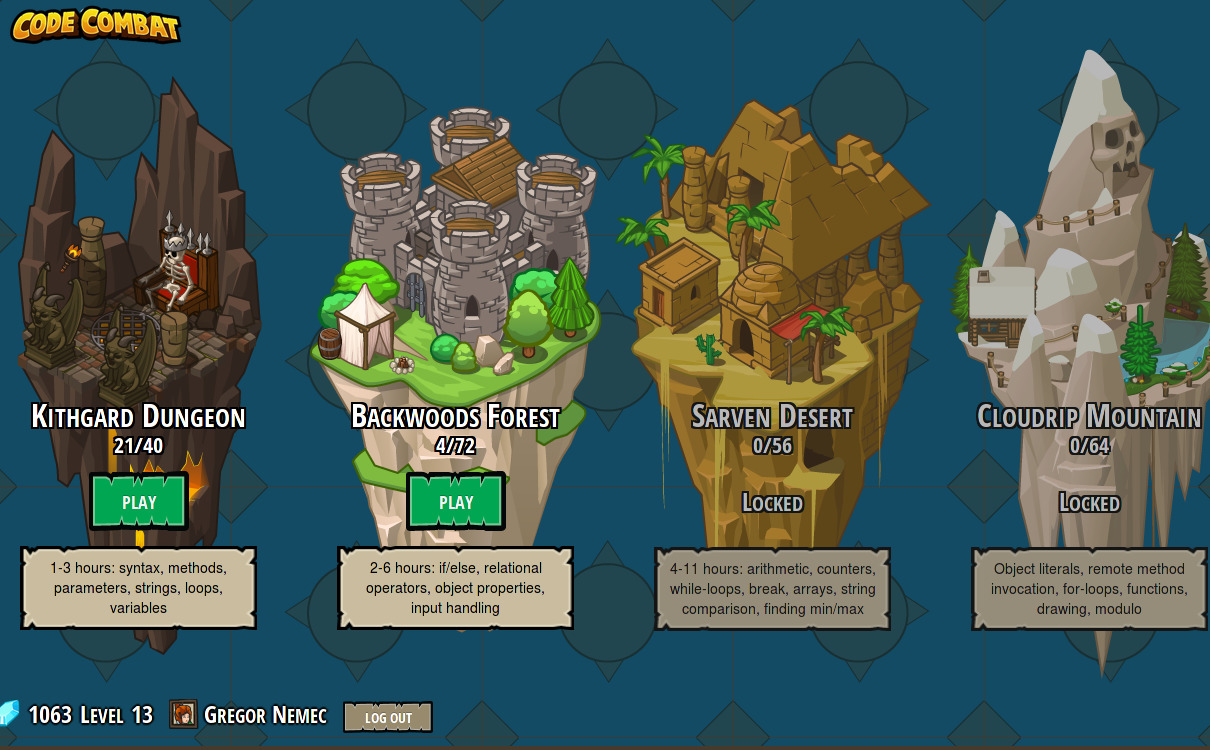
\includegraphics [width=0.65\linewidth, keepaspectratio =
   1] {./images/sc_web/cc_izbor-zem-v01.jpg}
   \caption{Izbor zemljevida na katerem bomo reševali naloge
     \cite{web:codecombat}.}
   \label{fig:web:cc:zemljevid}
 \end{figure}

 Igra se zgleduje po tipu iger igranja vloge (\emph{ang. Role play
   game - \textbf{RPG}}). Z junakom napredujemo po zemljevidu z vsako
 opravljeno nalogo, ob koncu vsake naloge prejmemo \textbf{točke -
   izkušnje} in napredujemo v lastnih \textbf{stopnjah}. Junak nabira
 številne predmete, ki mu omogočajo nadgradnjo veščin in tako lažje
 napredovanje skozi misije. Za začetek naloge pritisnemo na rdeče
 obarvan krog na zemljevidu (slika \ref{fig:web:cc:zemljevid:BG}),
 prikaže se povzetek naloge in katere koncepte bomo uporabili pri
 reševanju naloge. 

\begin{figure}[h!]
  \centering
    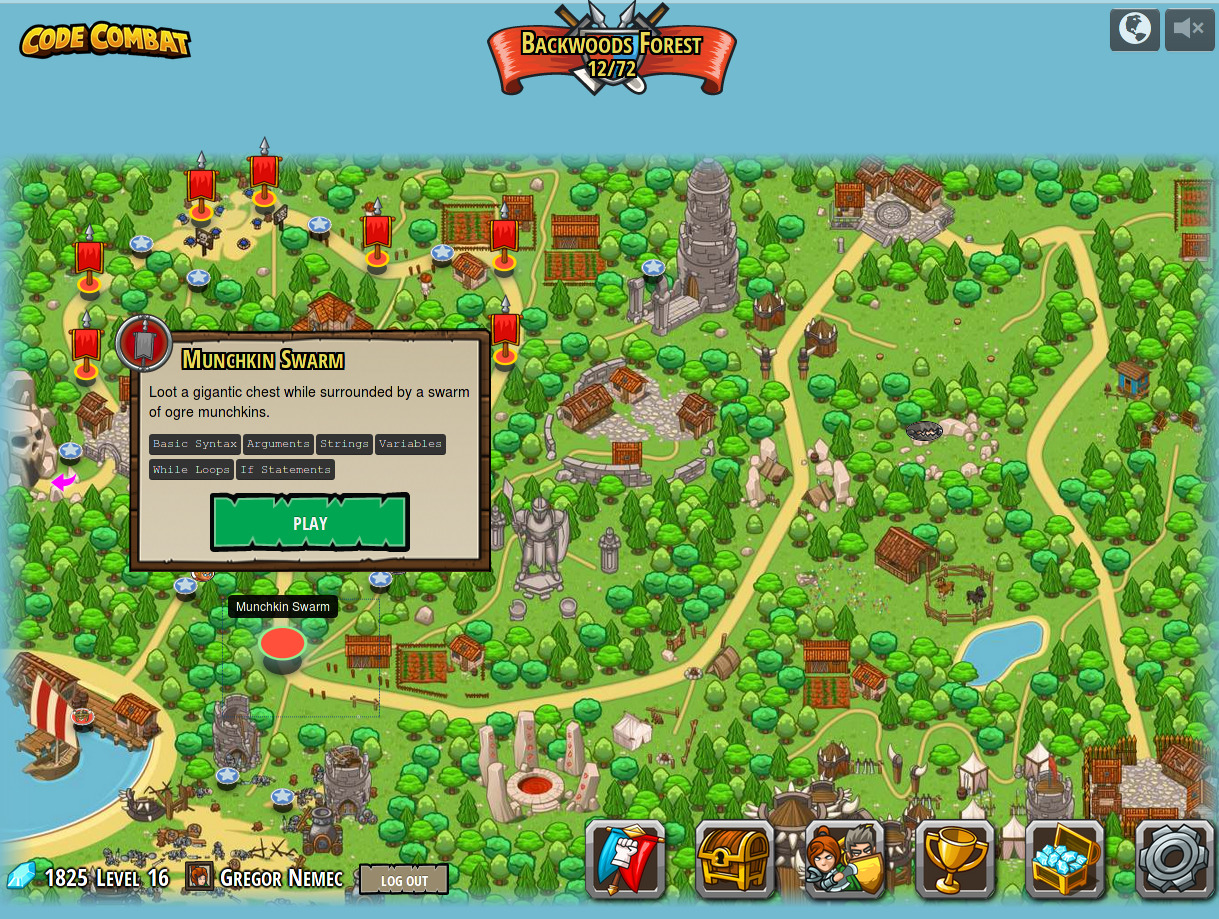
\includegraphics [width=0.65\linewidth, keepaspectratio =
   1] {./images/sc_web/cc_izbor-zem-BG-v01.jpg}
   \caption{Podroben zemljevid za izbiro nalog \cite{web:codecombat}.}
   \label{fig:web:cc:zemljevid:BG}
 \end{figure}

 Sledi opremljanje junaka (slika \ref{fig:web:cc:zemljevid:EQ}). Igra
 tu pomaga v tolikšni meri, da omeji nekatere predmete, ki niso
 uporabni za trenutno nalogo. Seveda sledimo logiki igre in izbiramo
 veno najboljšo opremo, ki je na voljo.
 
\begin{figure}[h!]
  \centering
    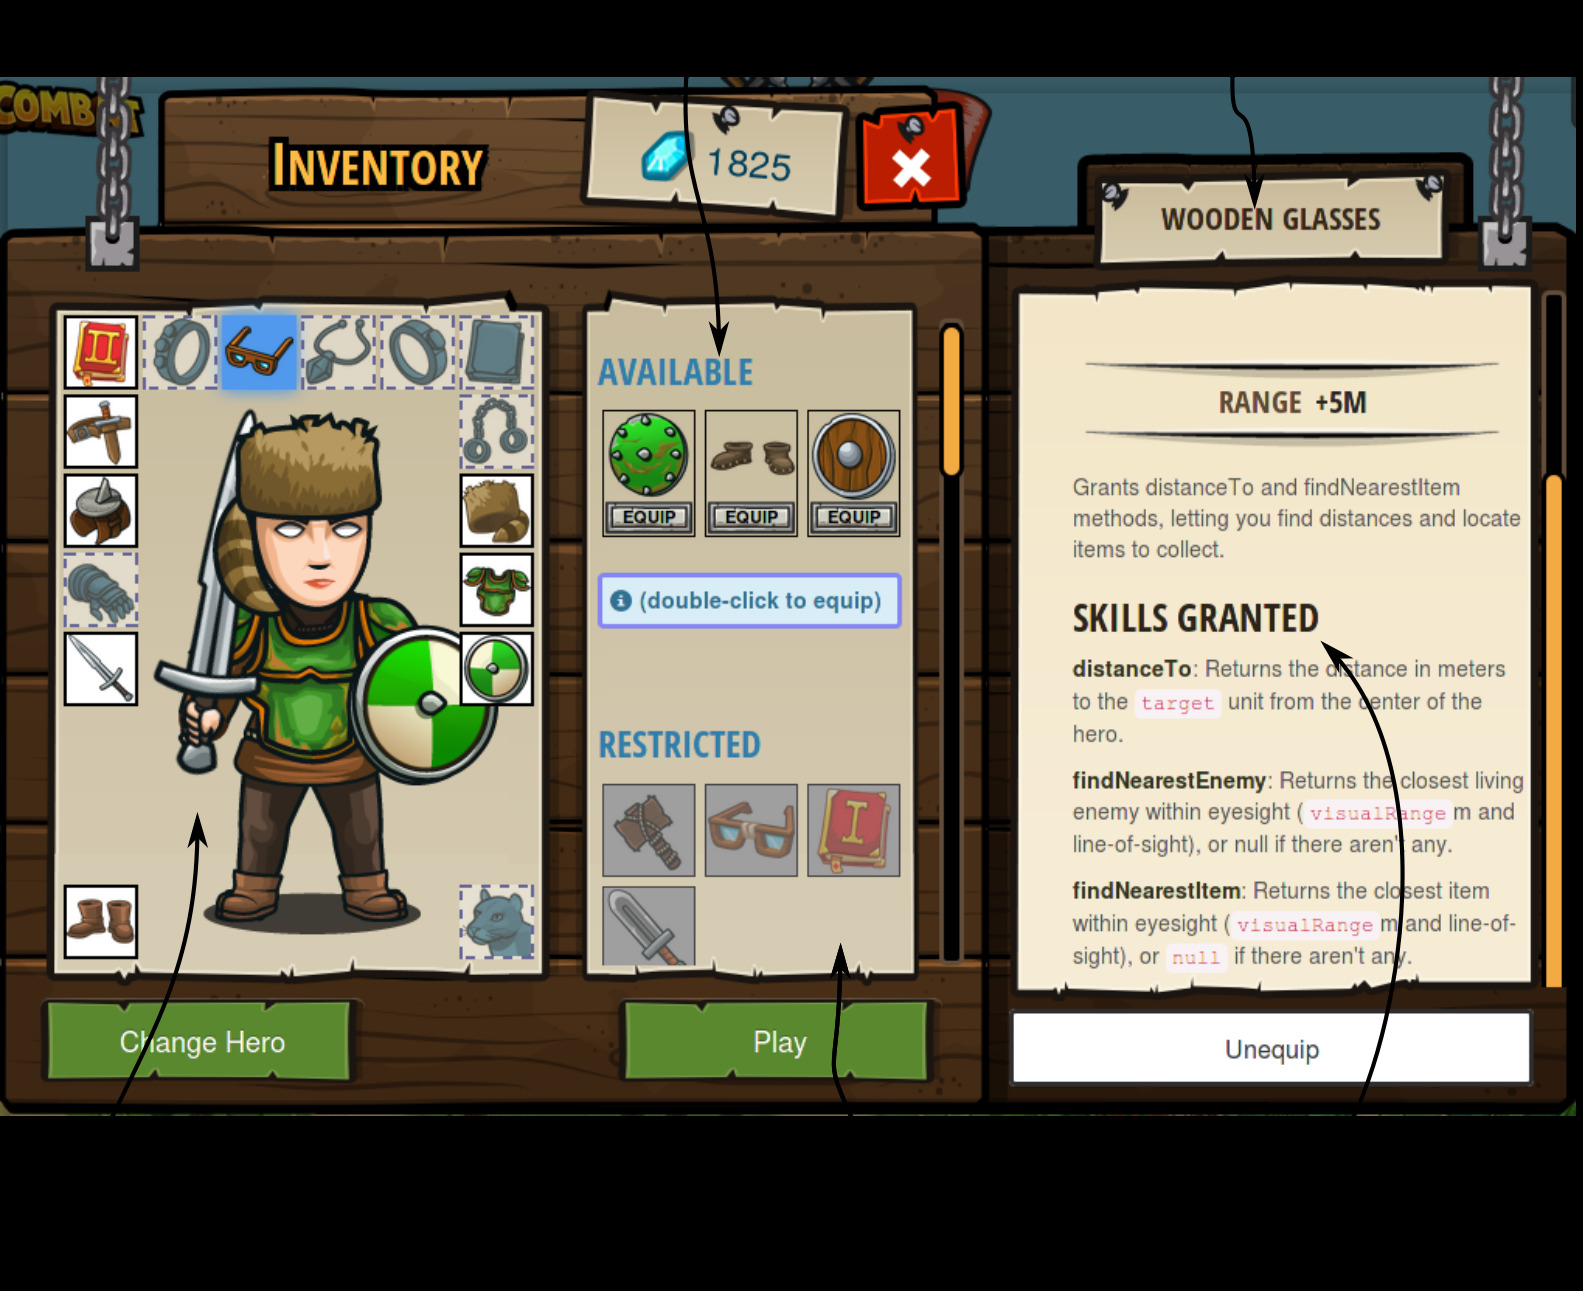
\includegraphics [width=0.55\linewidth, keepaspectratio =
   1] {./images/sc_web/cc_izbor-zem-EQ-v01.jpg}
   \caption{Oprema junaka in njen opis \cite{web:codecombat}.}
   \label{fig:web:cc:zemljevid:EQ}
 \end{figure}
 
 Ko kažemo ta primer igre smo z napredkom rešenih nalog skoraj na
 polovici drugega zemljevida in so oprema in veščine, ki jih uporablja
 naš junak že napredne, zato naredimo primerjavo med prejšnjo in
 nadgrajeno opremo. Z primerjave škornjev (slika \ref{fig:cc:eq:sb} in
 \ref{fig:cc:eq:lb}) lahko lahko povzamemo katere metode je junak
 pridobil, Če je pri \emph{enostavnih škornjih} imel možnost gibanja
 le v smeri \textbf{levo, desno, gor in dol} se lahko pri
 \emph{usnjenih škornjih} giblje po najkrajši poti na koordinate, ki
 jih podamo kot argument metode \texttt{hero.moveXY(x,z)}. S
 primerjavo \emph{knjige za programiranje} med verzijo \emph{I in II}
 (slika \ref{fig:cc:eq:p1} in \ref{fig:cc:eq:p2}), ki smo jo pridobili
 kasneje je razlika med veščinami očitna. Če smo pri \emph{knjigi za
   programiranje I} lahko uporabljali samo zanke
 \texttt{\textbf{loop:}} oz. \texttt{\textbf{while True}:}, pri
 \emph{knjigi za programirane II} lahko zraven še uporabljamo
 \texttt{\textbf{if/else stavek}}. Primerjali smo samo dva predmeta,
 junaku so na voljo, številni predmeti z različnimi metodami za
 različne dele telesa, vse od \textbf{mečev, ščitov, kap, ur, pasa,
   obleke, očal} in tako dalje. Z napredovanjem veščin in naborom
 predmetov junak pridobiva na zmožnostih, prav tako se s tem postopno
 izboljšujejo veščine in se širi znanje uporabniku spletne igre.

 \begin{figure}[h!]
    \centering
    \begin{subfigure}[]{0.25\textwidth}
      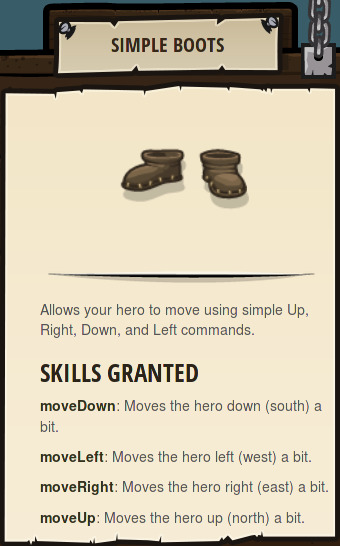
\includegraphics[width=\textwidth]{./images/sc_web/cc_EQ-SB-v01.jpg}
        \caption{Enostavni škornji (\emph{ang. Simple boots})}
        \label{fig:cc:eq:sb}
      \end{subfigure}
      \qquad
    \begin{subfigure}[]{0.25\textwidth}
        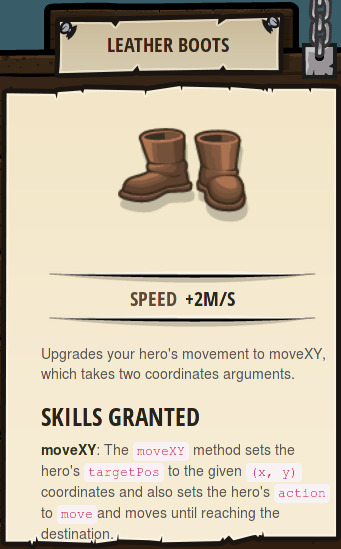
\includegraphics[width=\textwidth]{./images/sc_web/cc_EQ-LB-v01.jpg}
        \caption{Usnjeni škornji (\emph{ang. Lether boots})}
        \label{fig:cc:eq:lb}
    \end{subfigure}
    \\
    \begin{subfigure}[]{0.25\textwidth}
      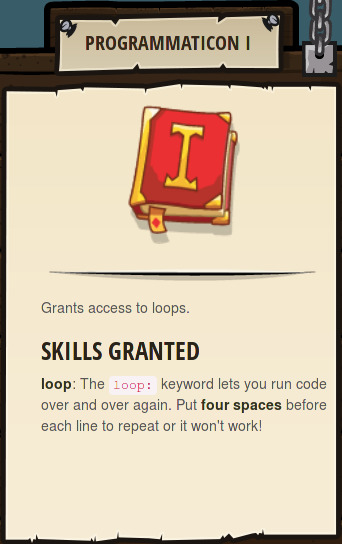
\includegraphics[width=\textwidth]{./images/sc_web/cc_EQ-P1-v01.jpg}
        \caption{Knjiga programiranja I}
        \label{fig:cc:eq:p1}
      \end{subfigure}
      \qquad
    \begin{subfigure}[]{0.25\textwidth}
        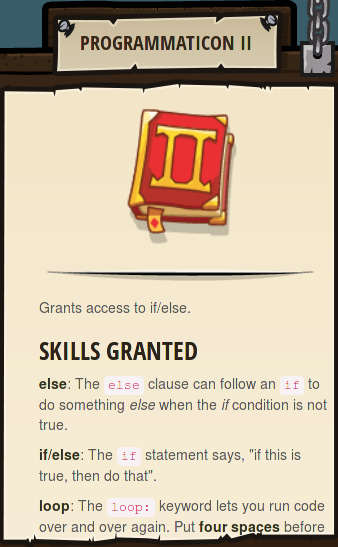
\includegraphics[width=\textwidth]{./images/sc_web/cc_EQ-P2-v01.jpg}
        \caption{Knjiga programiranja II}
        \label{fig:cc:eq:p2}
    \end{subfigure}
    \caption{Primerjava med prejšnjo različico opreme in njeno
      nadgradnjo, ki jo lahko zamenjamo junaku \cite{web:codecombat}.}
   \label{fig:web:cc:EQ:Primerjava}
\end{figure} 

%(slika \ref{fig:web:cc:ingame:cilji})
% \begin{figure}[h!]
%   \centering
%     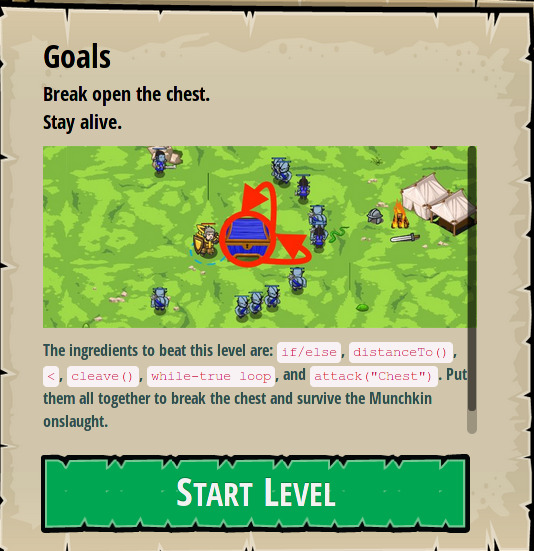
\includegraphics [width=0.35\linewidth, keepaspectratio =
%    1] {./images/sc_web/cc_ingame-goals-v01.jpg}
%    \caption{Prikaz ciljev v začetku igre \cite{web:codecombat}.}
%    \label{fig:web:cc:ingame:cilji}
%  \end{figure}

Po vsakem zagonu igre sledi najprej prikaz cilja , ki ga moramo
uresničiti. Postavitev igre (slika \ref{fig:web:cc:ingame:game}) je
taka, da nalogo rešujemo v \textbf{urejevalniku besedil}, ki je na
desni strani zaslona. Programska koda, ki jo izvajamo se odvija v oknu
na levi strani. Urejevalnik besedil omogoča nekatere napredne
funkcije, kot je \textbf{barvanje kode, samodejno zamikanje vrstic,
  prikaz zamika vrstic, sprotno opozarjanje na napačno sintakso} ter
\textbf{predlogi za samodejno dokončevanje} programske kode. Pri samem
pisanju programske kode lahko zapišemo na primer samo del metode, kot
je \texttt{find} in se nam ob potrditvi samodejnega predloga izpiše
celotna programska koda \texttt{enemy = hero.findNearestEnemy()}.

\begin{figure}[h!]
  \centering
    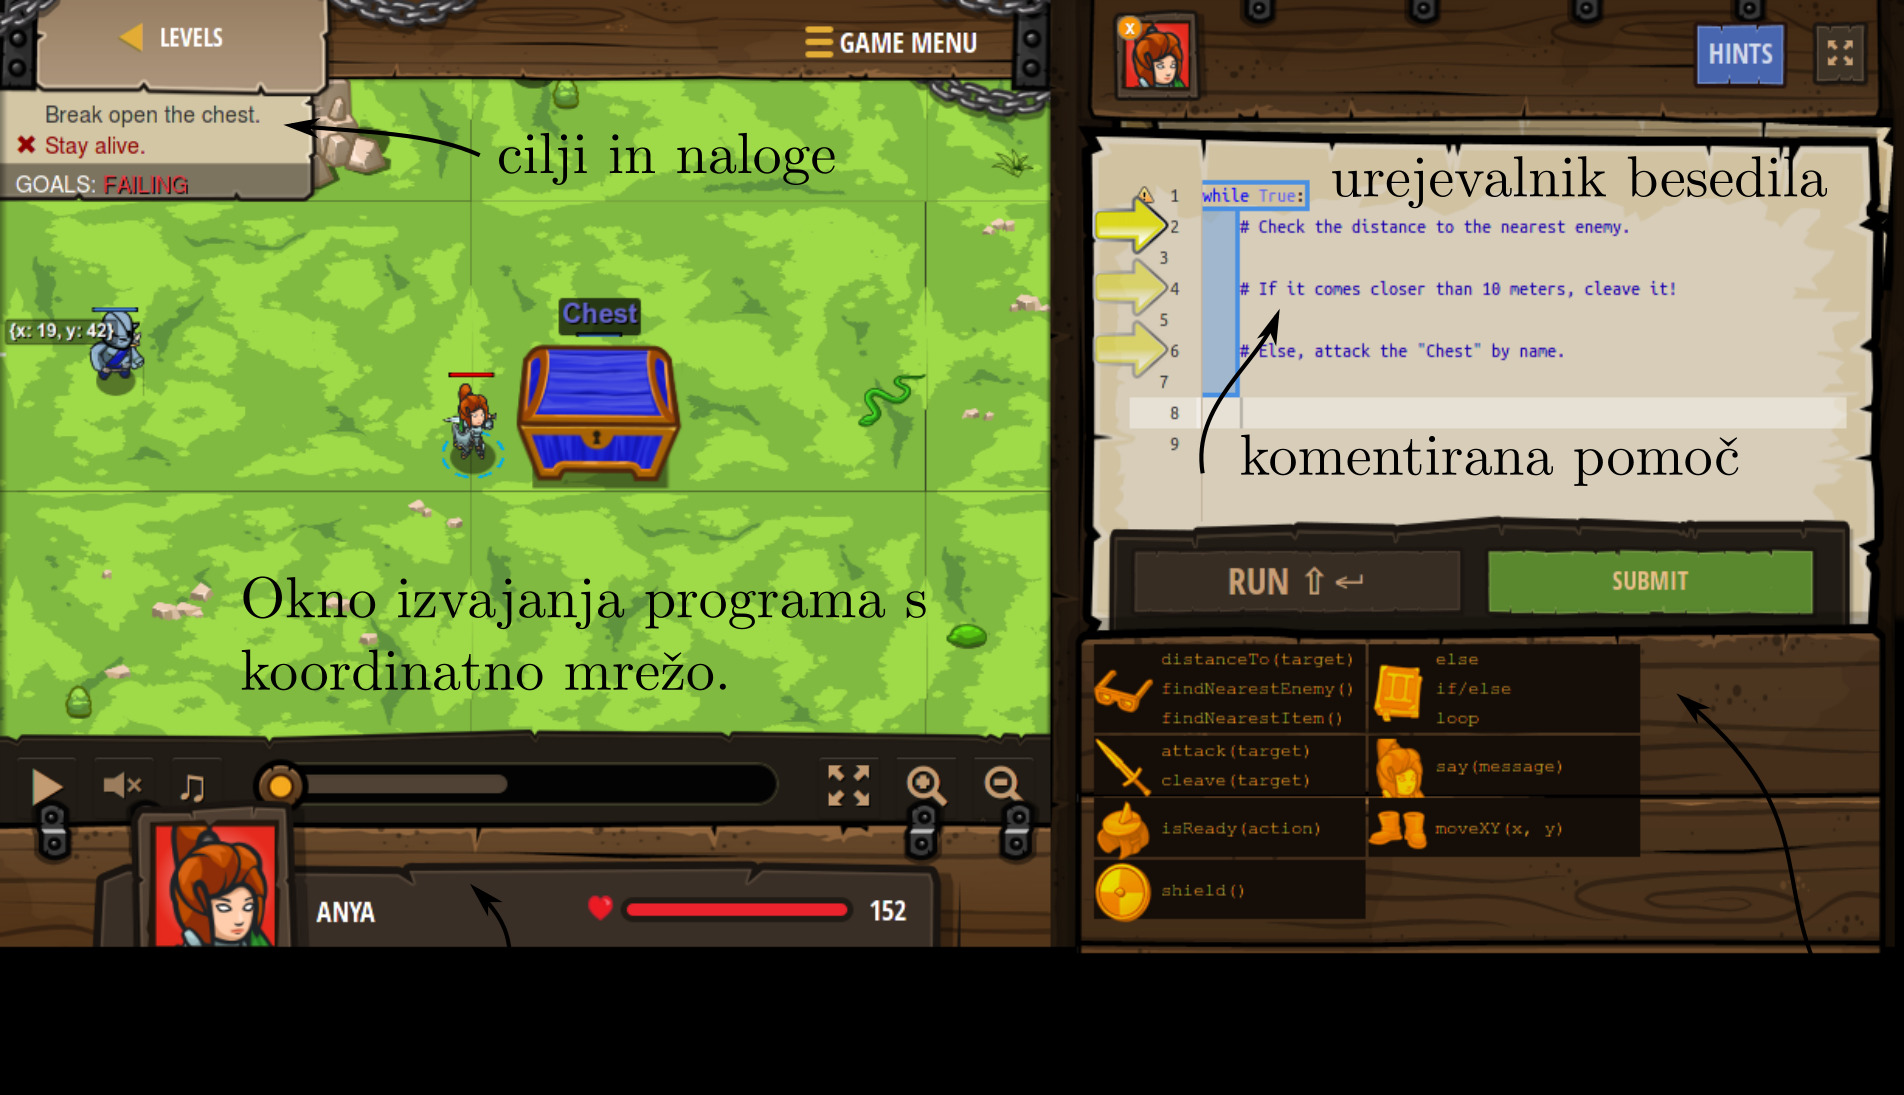
\includegraphics [width=0.55\linewidth, keepaspectratio =
   1] {./images/sc_web/cc_ingame-game-v01.jpg}
   \caption{Postavitev igre \cite{web:codecombat}.}
   \label{fig:web:cc:ingame:game}
 \end{figure}

 V trenutni nalogi je cilj tak, da moramo napadati sovražnike, ko je
 ta bližje skrinji kot \emph{10m} in ga moramo napasti z metodo
 \texttt{cleve}, če ga sovražnika ni v bližini napadamo skrinjo. Ko
 smo zadovoljni s svojo rešitvijo poženemo program in čakamo na končan
 izid (slika \ref{fig:web:cc:ingame:game2}). Če je iztek programa
 uspešen in smo rešili nalogo, jo \emph{posredujemo}.

\begin{figure}[h!]
  \centering
    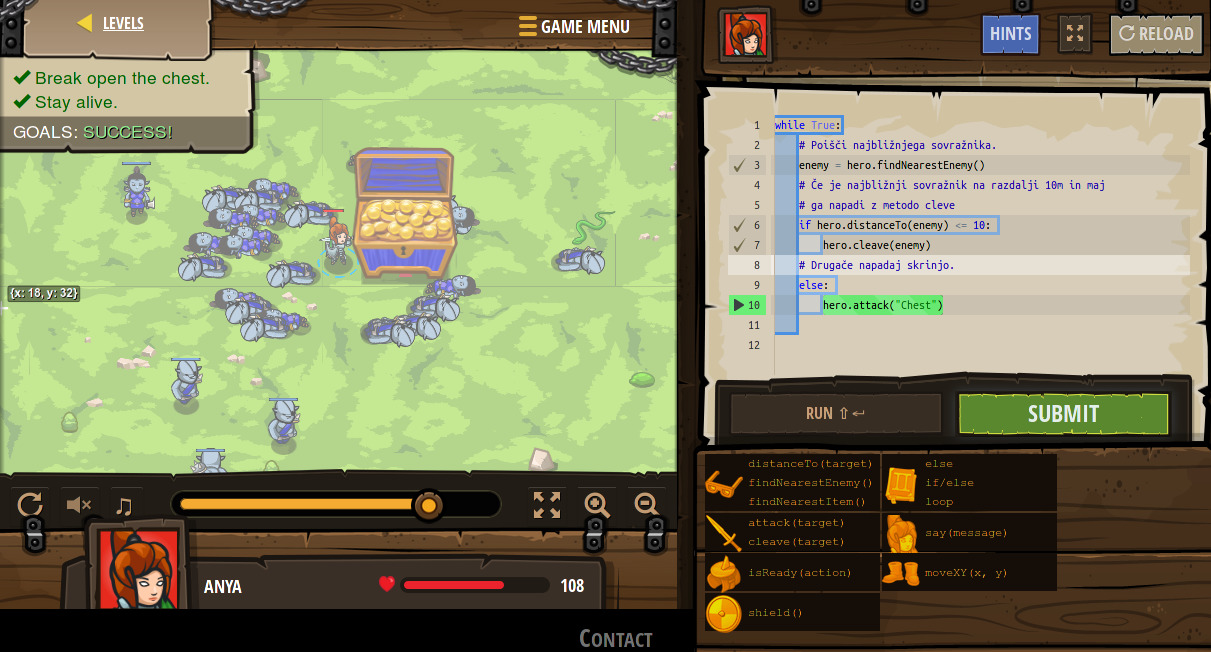
\includegraphics [width=0.55\linewidth, keepaspectratio =
   1] {./images/sc_web/cc_ingame-game-v02.jpg}
   \caption{Uspešno končan izid igre s napisano programsko
     kodo \cite{web:codecombat}.}
   \label{fig:web:cc:ingame:game2}
 \end{figure}
 
 Ob koncu igre poberemo še \textbf{dosežke}, to so \textbf{točke
   izkušenj}, \textbf{diamante} in \textbf{značke} (slika
 \ref{fig:web:cc:ingame:ach}) . 

\begin{figure}[h!]
  \centering
    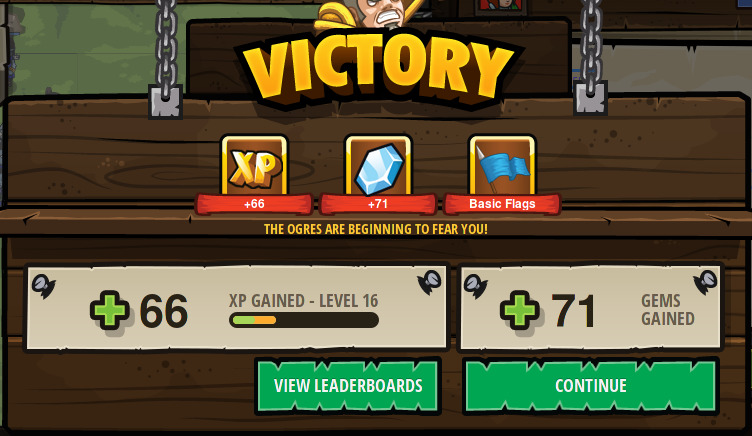
\includegraphics [width=0.35\linewidth, keepaspectratio =
   1] {./images/sc_web/cc_ingame-ach-v02.jpg}
   \caption{Končni rezultat in pregled nad dobljenimi dostžki ob koncu
     igre\cite{web:codecombat}.}
   \label{fig:web:cc:ingame:ach}
 \end{figure}

 Dostop do spletnega portala pa ni povsem brezplačen. Z
 \textbf{brezplačnim dostopom} lahko raziščemo 145 nalog v petih
 zemljevidih. Spletni portal ponuja \textbf{naročnino} 10\$\/mesec, s
 katero lahko pridobimo dodate \textbf{naloge, junake, diamante} in
 tako dalje.
 
\subsubsection{Upravljanje razreda}
\label{sec:upravljanje_razreda}

Spletni portal omogoča \textbf{upravljanje razredov}. Razrede upravlja
\textbf{učitelj}.  Portal ima prilagojeno učno snov za tri stopnje po
ameriškem \textbf{K-12} sistemu. Kot smo že primerjali šolske sisteme
lahko povemo, da so stopnje po starosti v slovenski šoli prilagojene
na naslednje stopnje \textbf{osnovno šolo (2.triado in 3. triado) in
  srednjo šolo}. Upravljanje razredov (slika \ref{fig:web:cc:teach})
je podobno kot smo to videli pri \textbf{Code academy} v poglavju
\ref{sec:uporaba_v_soli}. Učitelj ima nadzor nad dodajanjem učencev in
ima pregled o napredku učencev. Z njimi preko portala ne more
komunicirati.

\begin{figure}[h!]
  \centering
    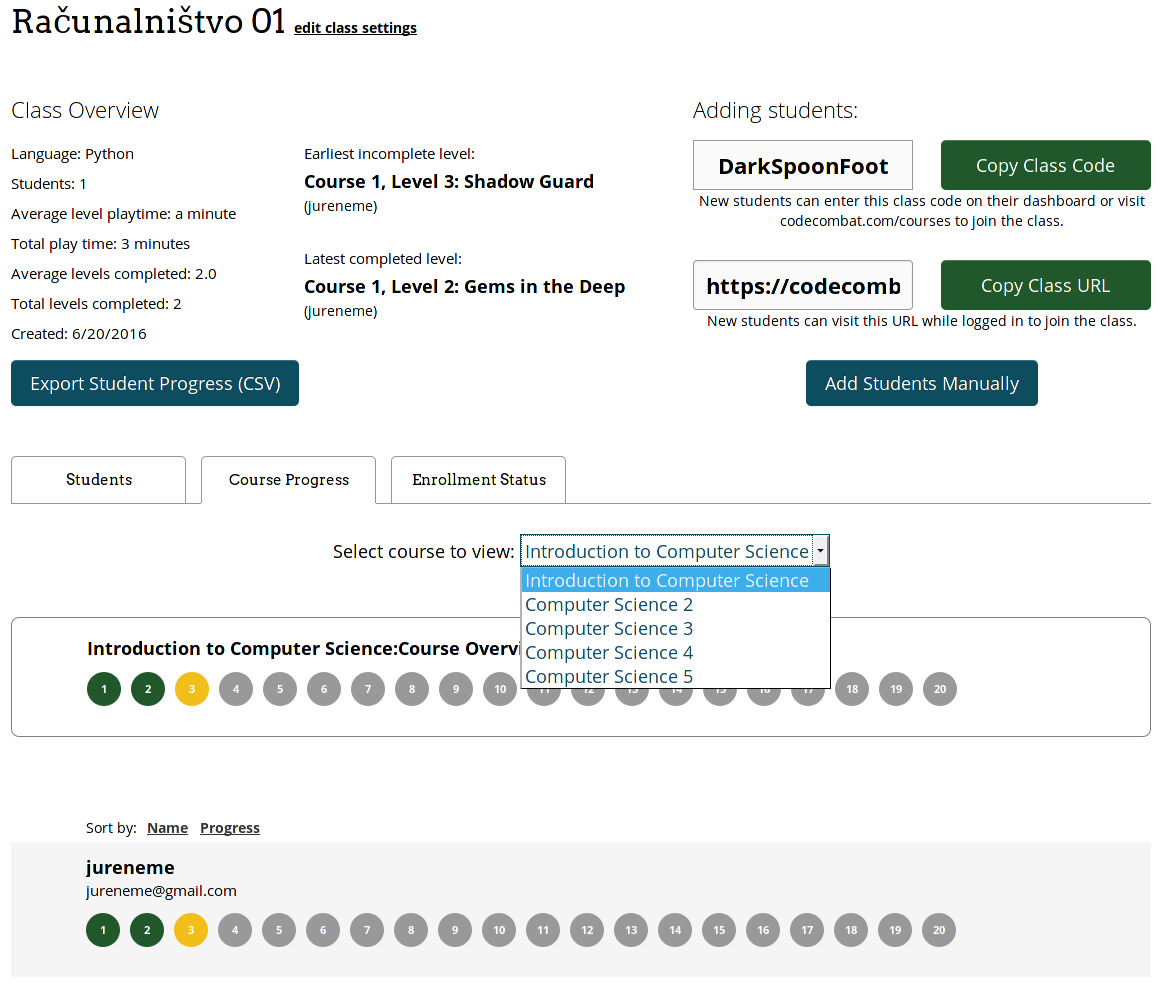
\includegraphics [width=0.75\linewidth, keepaspectratio =
   1] {./images/sc_web/cc_teach-clsv-v01.jpg}
   \caption{Učiteljev pogled na upravljanje razreda \cite{web:codecombat}.}
   \label{fig:web:cc:teach}
\end{figure}

Dostop \textbf{za šole ni brezplačen}. Učitelj lahko zahteva
demonstracijsko različico in v njo povabi neomejeno število učencev. V
tej demo različici je na voljo samo prvi tečaj \textbf{Uvod v
  računalniško znanost}, vsi ostali so zaklenjeni. Za uporabo
nadaljevalnih tečajev mora učitelj zaprositi za poizvedbo cene za nakup
licence za posameznega učenca.

Učenec rešuje naloge podobno kot smo to lahko videli pri navadnem
računu, vendar ne more stopenj izbirati iz mape. Naloge oz. stopnje,
ki jih rešuje so prilagojene tečaju v katerega ga je vpisal
učitelj. Po opravljeni nalogi, učenec takoj nadaljuje na naslednjo
stopnjo kot je ta predvidena v tečaju. Učenec ima vpogled na naloge,
ki ga čakajo v tečaju. V seznamu lahko izbere tiste naloge, ki jih je
že opravil oz. tisto zadnjo v kateri je ostal. Za nadaljevanje mora
učenec rešiti prejšnjo nalogo. Če v navadnem računu lahko menjujemo
različne dele oblačil in opreme, je to v načinu učenčevega načina
onemogočeno. Učenčev lik ima navojo stvari, ki jih potrebuje pri
rešitvi naloge. S to omejitvijo je olajšano delo učitelja saj se tako
lahko razred osredotoči le na reševanje naloge.

 %(slika \ref{fig:web:cc:stud})
% \begin{figure}[h!]
%   \centering
%     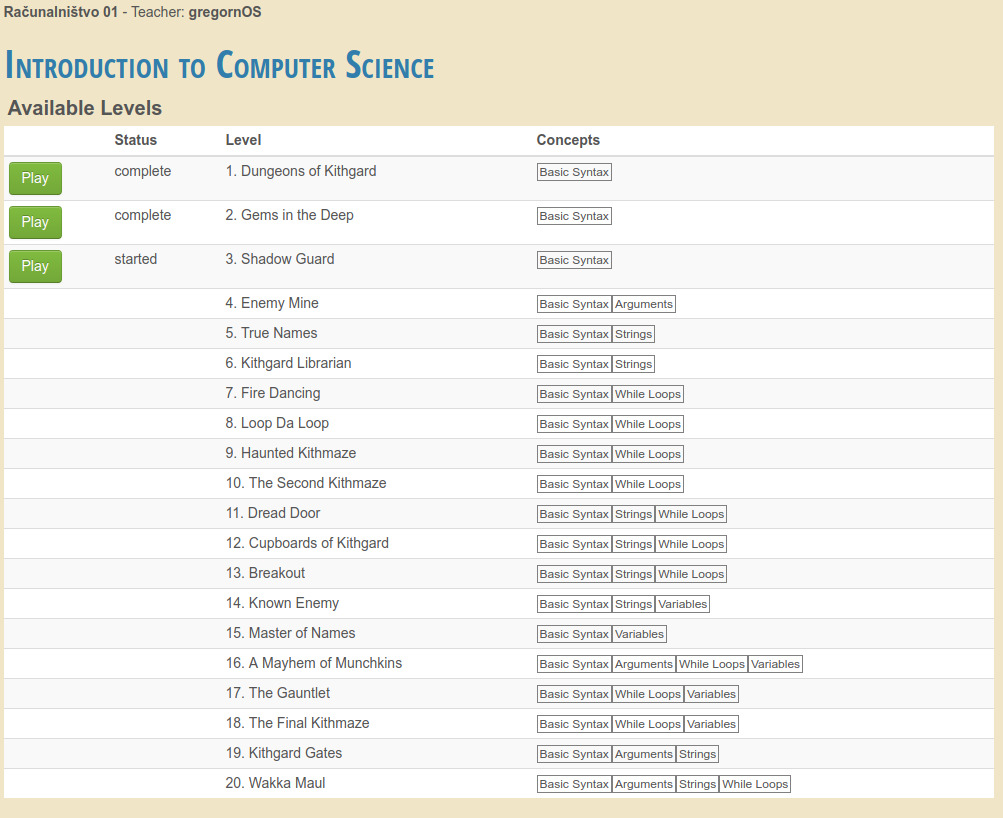
\includegraphics [width=0.65\linewidth, keepaspectratio =
%    1] {./images/sc_web/cc_stud-al-v01.jpg}
%    \caption{Učencev pogled na seznam nalog v tečaju \cite{web:codecombat}.}
%    \label{fig:web:cc:stud}
% \end{figure}

 Spletni portal ima prevode v več večjih svetovnih jezikov, žal
 trenutno slovenščina ni med njimi. V padajočem meniju, kjer učenci
 lahko spreminjajo jezike se najde tudi slovenščino, vendar se ob
 njenem izboru prikaže pojavno okno z pozivom za prevod v izbran
 jezik. Uporabniku se ponudi spremenjen račun, ki omogoča prevajanje v
 druge jezike. Torej obstaja neko upanje, da se bo mogoče nekoč nekdo
 lotil tega projekta in začel prevajati spletni portal in naloge v
 slovenski jezik. 

\subsubsection{Povzetek}
\label{sec:povzetek:codincombat}

Spletni portal oz. spletna igra ima vsekakor veliki motivacijski
faktor. Naloge so narejene sistematično in postopno. Če prav se v
naših osnovnih šolah ne priporoča učenje programskih jezikov, kjer
pišemo programsko kodo razen morda \textbf{Logo}. Naj bi se
uporabljali vizualni programski jeziki kot je \textbf{Scratch}. Za ta
spletni portal verjamem, da bi ga lahko uporabili pri osnovno šolcih,
kater bi lahko poučevali \textbf{Python}. Težava je edino, kot vedno
\textbf{slovenščina}, saj na strani še ni prevoda nalog in
\textbf{plačljivost} za uporabo razredov. To učitelj sicer lahko
zaobide z uporabo \textbf{navadnih računov} in uporabo brezplačnih
vsebin, vendar mu to uteži delo. 

\begin{osebnabox}[label={osebna:replIT}]{Repl.it | \url{https://repl.it/}}
    \begin{tabular}{
  p{0.30\linewidth-2\tabcolsep} |
  p{0.70\linewidth-2\tabcolsep}  }
  \textbf{Vrsta vsebine} & Spletna igra za programiranje. Kombinacija
                           igre RPG + pisanje programske kode. \\
      \hline
  \textbf{Jezik spletne strani} & angleščina: da, slovenščina: ne,
                                  drugi: da. \\
      \hline
  \textbf{Ponujena znanja} & Znanja programskih jezikov in  algoritmov. \\
      \hline
 \textbf{Programski jeziki} & Python, JavaScript, CoffeScript, LUA \\  
      \hline
  \textbf{Težavnostna stopnja} & Osnovno šolo (2/3 in 3/3) in srednjo
                                 šolo. \\ 
      \hline
   \textbf{Upoštevanje načel} & Problemski pristop: da,
                                sistematičnost: da, postopnost: da. \\
      \hline
  \textbf{Dosežki/Gamification} & Da (Značke, izkušnje, diamanti) \\
      \hline
  \textbf{Dodajanje lastnih vsebin} & Ne. \\
      \hline
  \textbf{Upravljanje razreda} & Da (Za osnovni tečaj brezplačno za
                                 ostale tečaje plačljiva licenca) \\ 
      \hline
  \textbf{Dostop vsebin} & Pol plačljiv: brezplačnih je 145 nalog,
                           plačljive so dodatne naloge 95, dodatni
                           diamanti, … za (9,99\$/mesec).   \\  

\end{tabular}
\end{osebnabox}

\subsection{Codingame}
\label{sec:codingame}

Spletni portal \emph{\href{https://www.codingame.com}{Codingame}}
\cite{web:codingame} je spletna igra, katere bistvo je da uporabnik
rešuje probleme, ki so zahtevni in so predstavljeni kot izzivi v
obliki igre. Uporabnik z podajanjem rešitev izboljšuje veščine
programiranja in znanje algoritmov.

Za vsakega uporabnika se igranje oz. reševanje problemov začne pri
\textbf{sestavljankah} (\emph{ang. puzzles}) (slika
\ref{fig:web:ca:puzz}). V eno igralskem načinu so igre razdeljene na
več težavnosti vse od \textbf{lahkih} do \textbf{zelo težkih}. Na tej
strani lahko izbiramo med sestavljankami, kjer imamo nalogo, da
programsko kodo čim bolj \textbf{optimiramo}
(\emph{ang. optimisation}) , torej poiščemo rešitev, ki potrebuje
najmanjšo časovno in prostorsko zahtevnost. Druga vrsta iger je taka
da z čim manj kode, torej znanjem trikov programskega jezika rešimo
problem, na strani \emph{ang. Code golf}. Imamo še možnost, da
rešujemo naloge, ki jih je pripravila skupnost, na strani
\emph{ang. Community puzzles}. Na tej strani se lahko posredujejo
lastne naloge, ki pa morajo biti odobrene s strani razvijalcev spleten
strani preden se lahko objavijo.  

\begin{figure}[h!]
  \centering
    \includegraphics [width=0.75\linewidth, keepaspectratio =
   1] {./images/sc_web/codingame_puzz-v01.jpg}
   \caption{Podstran \emph{\href{https://www.codingame.com}{Codingame}}
\cite{web:codingame} - sestavljanke.}
   \label{fig:web:ca:puzz}
 \end{figure}

 Poglejmo kako rešujemo problem. V ta name smo izbrali sestavljanko
 \textbf{Most - Episoda I} (\emph{ang. The bridge - Episode I}) (slika
 \ref{fig:web:ca:solve}). Za reševanje naloge lahko izbiramo med
 številnimi programskimi jeziki, kot so \textbf{C\#, C++, Java,
   JavaScript, Python3, Bash, C, Clojure, Dart, F\#}. V našem primeru
 bomo uporabili programski jezik \textbf{Python3}.
 
 Primer izbrane naloge pravi, da moramo napisati program, ki upravlja
 hitrost motorja, kateri se vozi po mostu in mora preskočiti prepad
 ter se na koncu pravočasno ustaviti. Celoten program teče v neskončni
 \texttt{while True} zanki. Na vsakem koraku moramo izpisati kaj je
 naslednja akcija motorja ali ta naj \texttt{POSPEŠI, ČAKA, ZAVIRA}
 ali \texttt{SKOČI}. Na vsakem koraku se hitrost poveča oz zmanjša za
 1. \texttt{Hitrost} se na vsakem koraku odraža za razdaljo, ki je
 enaka hitrosti. Vhodni podatki programa so naslednji, \texttt{cesta},
 ki je razdalja pred \texttt{prepadom}, naslednji podatek je velikost
 \texttt{prepada} in razdalja \texttt{zaviralne poti}.

 Na levi strani zgoraj \textbf{opazujemo potek rešitve}. Levo v
 sredini so napisana \textbf{navodila}, ki natančno opišejo problem,
 \emph{vhodne podatke, omejitve } in pričakovan \emph{izpis programa}
 na vsakem koraku. Levo spodaj je \emph{ukazna vrstica}, na kateri
 spremljamo izpis programa in ki nam je v pomoč pri razhroščevanju.

 Na desni strani je \textbf{urejevalnik besedil}, v katerega pišemo
 rešitev oz program. Urejevalnik zna barvati programsko kodo,
 samodejno upošteva zamik programske kode in podaja samodejne predloge
 za metode, ki so vgrajene ko napišemo ``.''. V nastavitvah
 urejevalnika lahko izbiramo način, ki prilagodi vedenje in ga lahko
 nastavimo na \emph{klasičen, emacs} in \emph{vim} način. Izbiramo
 lahko med temno in svetlo barvno shemo. Nastavimo lahko samodejno
 zaključevanje oklepajev.

 Spodaj desno poganjamo program s \textbf{testnimi primeri}, ki
 rešitev testirajo v skrajnih mejah. Testi, ki so podani kot
 vhodni podatki, so narejeni tako, da onemogočajo, da bi napisali
 program, ki bi imel statično vgrajene rešitve. Ko rešitev prestane
 vse teste jo lahko posredujemo. 

\begin{figure}[h!]
  \centering
    \includegraphics [width=1\linewidth, keepaspectratio =
   1] {./images/sc_web/codingame_solving-v01.jpg}
   \caption{Reševanje sestavljanke \emph{The Bridge}
     \cite{web:codingame}}
   \label{fig:web:ca:solve}
 \end{figure}

 Pri reševanju problemov se uči tudi življenjski krog razvijanja
 programske opreme in strategije reševanja problemov, kot smo jih
 opisali v poglavju \ref{sec:strategije_reševanja_problemov}, saj
 \textbf{problem najprej analiziramo, izberemo pristop, problem
   razgradimo, razvijemo algoritem in testiramo njegovo
   pravilnost}. Ta postopek lahko ponavljamo v krajših korakih dokler
 ne pridemo do prave rešitve in ponovimo faze razvoja in testiranja
 algoritma več krat. Ko algoritem reši problem, se lahko ukvarjamo z
 njegovo \textbf{učinkovitostjo}, ki jo pridobimo z upoštevanjem
 lastnosti implementacije algoritmov torej časovne in prostorske
 zahtevnosti ter z značilnosti programskega jezika in njegovih
 zmožnosti. Na tak posreden način nas spletni portal uči programski
 jezik, saj rešitev od nas zahteva optimalno rešitev, ki jo lahko
 dosežemo s dobrim poznavanjem programskega jezika in njegovih
 knjižnic.

 Med reševanjem si lahko pomagamo z \emph{namigi} in \emph{pseudo
   kodo}. Ko je rešitev oddamo, sledi izračun točk in nagrad v obliki
 \textbf{točk izkušenj} in \textbf{značkami}. Uporabnik lahko brska
 med rešitvami drugih uporabnikov in tako nabira dodatno znanje.

 Na spletni strani obstajajo še drugi načini igranja. Lahko se
 včlanimo v različne igre, kjer programiramo \textbf{bot-a}, ki
 tekmuje z \textbf{umetno inteligenco} na pod strani
 \emph{ang. AI}. \textbf{Spopad kode} ali \emph{ang. Clash of code} je
 način v katerem do 8 igralcev tekmujejo eden proti drugemu v bojih po
 5 ali 10 minut. Vsak zase rešuje problem, na koncu zmaga najbolj
 točkovana rešitev. Spletni portal prireja tudi uradna
 \textbf{tekmovanja} na katerih se brezplačno registriramo. Izbiramo
 lahko med dvema sistemoma nagrajevanja, ali so nagrade v fizični
 obliki, kot je npr. 3D tiskalini, majice in podobno ali se odločimo
 za način, kjer se potegujemo za razgovor na določenem delovnem mestu,
 ki je takrat razpisano. Dober koncept prepoznavanja talentov in
 iskanja službe.
 
\subsubsection{Povzetek}
\label{sec:povzetek_codingame}

Spletni portal je namenjen predvsem k treniranju veščin programiranja
in učenju algoritmov. Uporabnik zato mora poznati več kot so le osnove
programiranja, zato je spletni portal namenjen predvsem za srednje
šole, višje in univerzitetne programe študija. Spletna igra ni
primerna za pouk, je pa lahko zelo dobro dopolnilo za dodatno vajo ter
izpopolnjevanje lastnih izkušenj programiranja. Priporočamo ga lahko
vsakemu, ki ga zanima programiranje. Sistem nalog in reševanja teh je
dobro zasnovan. Problemsko je zasnovano tudi ozadje vsake
naloge. Naloge si po težavnosti sledijo postopoma, sistematično so
naloge razmetane po vseh težavnostih stopnjah, zato ne moremo potrditi
načela sistematičnosti. 

\begin{osebnabox}[label={osebna:codingame}]{Codingame |
    \url{https://www.codingame.com}}
    \begin{tabular}{
  p{0.30\linewidth-2\tabcolsep} |
  p{0.70\linewidth-2\tabcolsep}  }
  \textbf{Vrsta vsebine} & Vadnica: spletna aplikacija za
                           programiranje + reševanje problemov +
                           testiranje) \\
      \hline
  \textbf{Jezik spletne strani} & angleščina: da, slovenščina: ne,
                                  drugi: da. \\
      \hline
  \textbf{Ponujena znanja} & Znanje algoritmov in veščine programiranja. \\
      \hline
 \textbf{Programski jeziki} & C\#, C++; Java, JavaScript, Python3,
                              Bash, C, Clojure, Dart, F\# \\  
      \hline
  \textbf{Težavnostna stopnja} & Srednja šola, visoki, višji in
                                 univerzitetni. \\ 
      \hline
   \textbf{Upoštevanje načel} & Problemski pristop: da,
                                sistematičnost: na, postopnost: da. \\
      \hline
  \textbf{Dosežki/Gamification} & Da, značke, izkušnje, rangiranje \\
      \hline
  \textbf{Dodajanje lastnih vsebin} & Da. Dodajanje lastnih
                                      nalog/problemov, ki jih rešuje
                                      skupnost. \\
      \hline
  \textbf{Upravljanje razreda} & Ne. \\ 
      \hline
  \textbf{Dostop vsebin} & Brezplačno   \\  

\end{tabular}
\end{osebnabox}


%%% Local Variables:
%%% mode: latex
%%% TeX-master: "../diploma"
%%% End:

\newpage
\section{Možni načini uporabe spletnih portalov pri pouku}
\label{sec:načini_uporabe_sp}

V spodnjem sestavku izpostavimo nekatere skupne prednosti, ki jih
lahko prinese uporaba spletnih portalov za učenje programiranja pri
pouku. S pregledom spletnih portalov, ki so nastali na univerzah
(poglavje \ref{sec:SPUP}), in tistih, ki smo jih podrobno pregledali
(poglavje \ref{sec:pregled_spletnih_port}), lahko ugotovimo naslednje
prednosti.

\begin{description}
\tightlist
\item[Namestitev programske opreme ni potrebna], kar je zagotovo velika
  prednost. Mentorju praktično ni treba nameščati nobenega
  urejevalnika besedil, IDE, niti prevajalnika ali tolmača. Prav tako
  ni potrebe po nastavljanju sistemskih poti, ki jih mnogi
  prevajalniki zahtevajo. Uporaba SPUP je neodvisna od uporabe
  operacijskega sistema. Vsaka naprava, na kateri lahko poganjamo
  novodobni spletni brskalnik, omogoča uporabo SPUP. Učencem na domačih
  računalnikih ni treba namestiti nobene programske opreme. Na
  tem mestu bi poudarili, da mora biti učitelj previden pri dajanju
  domače naloge z uporabo računalnika. Zares se mora prepričati, da imajo to
  zmožnost vsi učenci. Najbolje je, da lahko vse dodatno delo, ki ga
  učitelj predvidi, učenci opravijo v šolski računalniški
  učilnici.
\item[Seznanjanje s programsko opremo] pri pouku ni potrebno. Znebimo
  se potrebe, da bi z novinci morali spoznavati urejevalnik besedil
  ali kompleksno IRO. Spoznavanje programskega jezika in reševanja
  problemov se lahko lotijo nemudoma.
\item[Pisanje progama od začetka do konca] ni potrebno. Večina
  spletnih portalov, ki ponujajo vsebine v obliki vadnice, imajo
  programske naloge pripravljene tako, da mora uporabnik vnesti le del
  programske kode. Za novinca to pomeni, da se osredotoči le na
  nalogo in del sintakse, ki jo v danem trenutku potrebuje, da reši
  zadano nalogo. To prednost smo že spoznali na SPUP avstralske
  univerze, kjer so uporabili tip naloge zapolni prazna mesta
  \cite{thesisAWebP}.
\item
\end{description}

Pripravili smo tudi konkretna primera za OŠ in SŠ, kako bi s spletnim
portalom lahko uresničili učne cilje, ki jih najdemo v učnem načrtu.

\subsection{Primer uresničevanja ciljev učnega načrta v osnovni šoli}
\label{sec:uresn-cilj-unega-os}

Učni načrt za računalništvo - neobvezni izbirni predmet
\cite{ucni_nacrt-neobvezni-izbirni-os} vsebuje vsebinski sklop
\textbf{Algoritmi}, ki smo ga povzeli v poglavju
\ref{sec:neobvezno_izbirni_predmet_rac}. Spletni portal
\emph{\href{https://codecombat.com/}{Code combat}}
\cite{web:codecombat} lahko učitelj uporabi pri\textbf{ ponovitvi
  sklopa}, ko je snov že predelal na primer s programskim jezikom in
spletnim orodjem \emph{\href{https://scratch.mit.edu/}{Scratch}}
\cite{web:scratch}. K obstoječim ciljem, ki so podani v učnem načrtu,
lahko dodamo še naslednje: \emph{učenci spoznajo osnove programskega
  jezika \textbf{Python}.}  Ker se učenci s pisanim programskim
jezikom srečujejo prvič, bi bilo dobro, da učitelj pripravi učne liste
s primerjavo med \emph{Scratchom} in sintakso \textbf{Pythona}
oz. metodami, ki se uporabljajo na portalu (slika
\ref{fig:primerjava:cc01}). V tem primeru niti ni pomembna podrobna
obravnava programskega jezika Python. Pomembno je, da učenci razumejo,
kaj posamezna vrstica programske kode izvrši, kateri del kode
predstavlja junaka in kateri akcijo junaka. To lahko pokažemo nazorno
z delom programske kode v \textbf{Scratchu} (slika
\ref{fig:primerjava:scr01}), ki ponazarja metode, ki jih uporabljamo
za vodenje junaka na spletni strani \emph{Codecombat} (slika
\ref{fig:primerjava:cc01}).

 \begin{figure}[h!]
    \centering
    \begin{subfigure}[]{0.35\textwidth}
      \includegraphics[width=\textwidth]{./images/sc_web/primerjava_scr-premiki-v01.jpg}
      \caption{Programska koda, napisana v
        \emph{\href{https://scratch.mit.edu/}{Scratchu}}
        \cite{web:scratch} za premikanje \emph{gor, levo, desno, dol}.}
        \label{fig:primerjava:scr01}
      \end{subfigure}
      \qquad
    \begin{subfigure}[]{0.35\textwidth}
        \includegraphics[width=\textwidth]{./images/sc_web/primerjava_cc-premiki-v01.jpg}
        \caption{Programska koda v \textbf{Pythonu} klica
          predpripravljene metode, ki premikajo junaka \emph{gor,
            levo, desno, dol}.}
          \cite{web:codecombat}
        \label{fig:primerjava:cc01}
    \end{subfigure}
    %Dodaj še za zanko
    % \\
    % \begin{subfigure}[]{0.25\textwidth}
    %   \includegraphics[width=\textwidth]{./images/sc_web/cc_EQ-P1-v01.png}
    %     \caption{Knjiga programiranja I}
    %     \label{fig:cc:eq:p1}
    %   \end{subfigure}
    %   \qquad
    % \begin{subfigure}[]{0.25\textwidth}
    %     \includegraphics[width=\textwidth]{./images/sc_web/cc_EQ-P2-v01.png}
    %     \caption{Knjiga programiranja II}
    %     \label{fig:cc:eq:p2}
    % \end{subfigure}
    \caption{Primerjava programskih blokov, napisanih v
      \textbf{Scratchu}, in enačic klica metod, napisanih v
      \textbf{Pythonu} na spletni strani \emph{Codecombat}.}
   \label{fig:primerjava:scrVScc}
\end{figure}

Kot smo že omenili v predstavitvi spletnega portala \emph{Codecombat},
ima učitelj dve možnosti:

\begin{itemize}
\tightlist
\item učenci uporabljajo svoje ustvarjene račune,
\item učitelj ustvari \textbf{demo} razred in v njega vključi učence.
\end{itemize}

Glavna slabost v prvem primeru je ta, da tako lastno ustvarjeni računi
učencev omogočajo izbiro junakov, predmetov, ki jih uporabljajo pri
reševanju nalog, in se zato lahko pri učni uri zaplete pri nadzoru
napredka pri posameznem učencu in je s tem delo učitelja oteženo. Zaradi
teh razlogov se bolj nagibamo k drugi možnosti.

Učitelj lahko s prošnjo zaprosi za \textbf{demonstracijski} račun, v
katerem ima možnost ustvariti razred s prvim vsebinskim sklopom
\textbf{Uvoda v računalniško znanost} (\emph{ang. Introduction to
  Computer Science }). To je edini sklop v tem načinu, ki je
brezplačen in ga lahko uporabimo v šoli pri nas brez dodatnih
stroškov. Učitelj učence povabi v razred z edinstveno ustvarjenim
\textbf{URL} naslovom. Registracija po kliku na povezavo je potrebna.
Učenci se od naloge do naloge premikajo brez povzetka prejema dosežkov, izbire predmetov in izbire opreme za svojega junaka. Za tako delo
je primeren tip učen ure \textbf{praktično vodeno delo}, kjer učitelj
delo vodi z vnaprej pripravljenimi učnimi listi primerjave programskih
blokov (slika \ref{fig:primerjava:scrVScc}) in povzetki navodil v
slovenščini. Ko učenci v začetnih nalogah osvojijo osnovne metode
junaka, lahko učitelj stopnjuje samostojnost dela učencev. Delo na
spletnem portalu je primerno za dvojno učno uro
oz. \textbf{90 min}. Tiste naloge, ki jih učenci ne uspejo dokončati,
jih lahko učitelj dodeli za domače delo.

Sklop vsebinsko predstavlja naslednje koncepte programiranja:
\textbf{osnove sintakse, argumente, spremenljivke, tip
  spremenljivke, \texttt{string}, \texttt{while} zanka}. Pri
preverjanju sklopa nekaterih operativnih ciljev ne moremo preveriti,
zapisali smo tiste, ki jih ni moč preveriti, in zakaj:

\begin{itemize}
\tightlist
\item \textbf{algoritem predstavijo simbolno (z diagramom poteka) ali s
  pomočjo navodil v preprostem jeziku}. Na spletni strani algoritmi
niso predstavljeni z diagrami, lahko jih sicer pripravi učitelj,
vendar v tej fazi to ni nujno potrebno;
\item \textbf{znajo v algoritem vključiti vejitev}. Uporaba vejitev v
  tem prvem sklopu \textbf{CS1} na spletnem portalu ni omogočena;
\item \emph{znajo uporabiti nekatere ključne algoritme za sortiranje in
  iskanje};
\item \emph{poznajo osnovne algoritme za iskanje podatkov}.
\end{itemize}

Menimo, da ostale cilje lahko uspešno povzamemo in preverimo v učni
uri ponovitve vsebinskega sklopa. Čeprav uporaba spletne igre
predstavlja kar nekaj priprave učitelja, ima izjemno motivacijsko
vrednost, ki lahko učence navduši za nadaljnje delo.

\subsection{Primer uresničevanja ciljev učnega načrta v srednji šoli}
\label{sec:prim-uresn-cil-ss}

Učni načrt \textbf{informatike} na programu splošne gimnazije
predvideva učenje algoritmov in programiranja pa ravni
\textbf{posebnih znanj} v tematskem sklopu obdelave
podatkov. Predpostavimo, da mentor oz. profesor informatike
uresničuje znanje algoritmov in programiranja, ta lahko uporabi
spletni portal \emph{\href{https://www.codecademy.com/}{Codeacademy}}
\cite{web:codeacademy} v namene domačega dela. Profesor mora
upoštevati medpredmetno povezovanje s predmetom angleščina in za dani
sklop pripraviti prevode navodil, ki so lahko dijakom v
pomoč. Prednost portala je še ta, da lahko vsebinske sklope in posamezne
teme, ki so na voljo, poljubno izbiramo ne glede na vrstni red
oz. na to, kaj smo že predelali. Kako lahko profesor izkoristi uporabo
sledenju napredka dijakov, smo že podrobno opisali v poglavju
\ref{sec:uporaba_učitelji}.

Spletni portal lahko uporabi pred obravnavo neke snovi in se tako
dijaki že seznanijo z določeno funkcionalnostjo in sintakso
programskega jezika. Ker dijaki že del znanja in sintakse usvojijo, so
naloge pri pouku lahko zahtevnejše in je lahko večji poudarek na
strategiji reševanja (težjih) problemov. Konkretno, za domače delo
lahko dijaki rešujejo nalogo \emph{``Strings \& Console Output''}, kjer
usvojijo osnovno znanje ravnanja s \textbf{pisanjem izhodnih podatkov}
in \textbf{podatkovnega tipa \texttt{string} oz. \texttt{niza}}. Naučijo se
uporabljati metode, ki jih ponuja podatkovni tip \texttt{string},
lepijo dve besedi skupaj in tako dalje. Kot že rečeno, z osvojenim
znanjem lahko pozneje pri pouku rešujejo zahtevnejše naloge.

V drugem primeru lahko ta portal uporabi po obravnavi določenega
vsebinskega sklopa in vadnico na portalu
\emph{\href{https://www.codecademy.com/}{Codeacademy}}
\cite{web:codeacademy} izkoristi, dijaki z domačim delom utrdijo svoje
znanje. Poglejmo konkreten primer. Dijaki na primer imajo  po
\textbf{obravnavi sklopa vhodni podatki, podatkovni tip,
  \texttt{string}} in \textbf{\texttt{if else} vejitve} 
zadostno znanje, da rešijo nalogo \emph{``PygLatin''}. Napisati morajo
program, ki sprejme besedo in jo pretvori po določenem pravilu
slovarja ter jo izpiše na zaslon. Naloga je razdeljena na več vadnic,
dijaki nalogo rešujejo korak po koraku. Napredek
reševanja naloge lahko spremlja profesor preko portala.

  %%% Local Variables:
  %%% mode: latex
  %%% TeX-master: "../diploma"
  %%% End:

\newpage
\section{Zaključek}
\label{sec:zakljuek}

V diplomskem delu smo najprej spoznali, da učenje računalniške
znanosti in programiranja spada v \textbf{primarno področje uporabe
  računalnika v izobraževanju}. Pri nas se je na splošnem
izobraževalnem področju uveljavila usmeritev, ki zagovarja
\textbf{splošno usposobljenost} za delo z računalnikom, kljub temu se
z računalniško znanostjo in programiranjem večina učencev prvič
srečaja pri izbirnih predmetih \emph{Urejanje besedil, Multimedija in
  Računalniška omrežja} in pri neobveznem izbirnem predmetu
\emph{Računalništva} v \textbf{OŠ}. Dijaki se srečajo s programiranjem
v 1. letniku pri predmetu \emph{Informatika}. Posebnost so strokovni
programi, katerim je osnova računalništvo in je poudarek na
programiranju dosti večji, kar smo spoznali pri pregledu učnega načrta
predmeta \emph{Računalništva} Tehniške gimnazije. Ugotovimo lahko da
je programiranje pri splošnih predmetih zastopano do te mere, da se
učenci oz. dijaki dotaknejo teh znanj, pri čemer je v bolj strokovnih
predmetih kot je pri \emph{Računalništvo} v OŠ in na programu Tehnični
gimnazije zastopano v vse podrobnosti.

Pri pregledu osnovnih pojmov smo spoznali kaj predstavljajo programske
paradigme in ugotovili, da danes prevladuje paradigma \textbf{objektno
  orientiranega} programiranja. Podrobneje smo predstavili značilnosti
programskih jezikov, ki so trenutno najbolj popularni in ti so
\textbf{Java, C++, JavaScript} in \textbf{Python}. Čeprav so v
slovenskem izobraževalnem prostoru na srednje šolskem nivoju prisotni
vsi omenjeni, se za začetnike priporoča uporaba \textbf{Python-a}. V
osnovni šoli bi se naj uporabljal programski jezik \textbf{Scratch},
ki uporablja grafičen način sestavljanja gradnikov. Pri spoznavanju
osnovnih konceptov programiranja smo pripravili nekaj primerov
programov, ki jih skušajo čim bolj nazorno predstaviti.

Pri proučevanju \textbf{aktivnega pristopa} smo spoznali, da pouk
računalništva mora biti pozitivno naravna in je naj znanje grajeno z
\textbf{aktivnim učenje}, torej učenci z lastnim delom odkrivajo in
gradijo miselni model. Pri tem so naj uporabljene
\textbf{konstruktivne metode} poučevanja. Za aktivno učenje je ravno
tako značilen problemsko naravnan pouk. Reševanje nalog
oz. raznovrstnih problemov je naravno prisoten pri poučevanju
računalniške znanosti, zato smo izpostavili \textbf{strategije
  reševanja problemov} in smo osnove korake podrobno
razdelali. Strategije reševanja problemov niso pomembne le za področje
računalništva temveč za mnoga področja tehničnih in znanstvenih
disciplin ter na sploh pri vsakdanjem življenju. Zanimalo nas ali so
vse te značilnosti pouka računalništva zajete tudi z uporaba spletnih
portalov.

Prvi spletni portali za učenje programiranja so nastali v akademskem
okolju na različnih univerzah po svet. Spoznali smo, da se študenti
novinci srečujejo vsepovsod s podobnimi težavami, kot je instalacija
in nastavitev programske opreme, uporaba IRO, uporaba sintakse
programskega jezika, razumevanje prevajalnika in tako
naprej. Pri vseh treh spletnih portalih, ki smo jih pregledali, smo
lahko strnili naslednje značilnosti, glavni del vsakega spletnega
portala je \textbf{spletna aplikacija za učenje programiranja
  (SAZP)}. Njene značilnosti so, da vsebuje \textbf{urejevalnik
  besedil, omogoča zagon napisanega programa, vrača povratne
  informacije o napakah ter izpis vhodno-izhodnih podatkov}. Drugi
elementi spletnega portala poleg SPZP so še \textbf{razdelane vsebine
  z nalogami, omogočena je komunikacija med mentorjem in novincem,
  omogočen je pregled nad napredkom novinca}.

Najzahtevnejši del tega diplomskega dela, je bilo iskanje kriterijev s
katerimi smo lahko spletne portale klasificirali in jih
ovrednotili. Najprej smo jih razdelili po vrsti vsebine in
ugotovili, da so najzanimivejše tiste vsebine, ki so
\textbf{kombinirane}. Kombinirane vrste vsebin smo razdelili na
\textbf{osnovne} in \textbf{napredne}, v slednjih se prepleta
\textbf{SPZP}, tekstovni ali/in video \textbf{vodiči} ter
\textbf{navodila}. Vsi ti elementi napredne kombinirane vsebine
tvorijo \textbf{vadnico}, ki je navadno osnovna enota neke učne teme.
Za posamezni spletni portal želimo določiti v katerem \textbf{jeziku}
je predstavljen, katera \textbf{znanja ponuja}, ali so to veščine
programiranja, znanja algoritmov, ali morda druga projektna znanja,
kot je izdelava spletne strani. Za vsak spletni portal smo zapisali,
učenje katerih \textbf{programskih jezikov} omogoča, kakšni
\textbf{težavnostni stopnji} je namenjen. Podrobneje so nas zanimala
ali spletni portali, tisti z vsebino znajo upoštevati nekatera
\textbf{učna načela}, kot je \textbf{problemski pristop, načelo
  sistematičnosti} in \textbf{načelo postopnosti}. Pri posameznem
spletnem portalu smo izpostavili ali ta uporablja \textbf{ocenjevanje,
dosežkov}, ki je značilno za video igre. Zanimalo nas je še ali
omogočajo spletni portali, da \textbf{dodajamo lastne vsebine} ter ali je
omogočeno \textbf{upravljanje razreda}. Nazadnje nas je zanimalo ali
so gradiva na spletnih portalih \textbf{brezplačna}, \textbf{pol
  plačljiva}, torej so nekatera gradiva ali storitve brezplačne druga
plačljiva in \textbf{popolnoma plačljive}.

Spletnih portalov, ki želijo poučevati računalniške znanosti in
programiranja je na spletu zarez veliko, zato smo morali določiti
omejitve s katerimi smo izbrali tiste, za katere smatramo, da nam bodo
pri pouku najbolj v pomoč. Te omejitve so naslednje, spletni portal
mora vsebovati \textbf{SAZP}, ki pa lahko nastopa tudi samostojno brez
vsebine, vrsta vsebin naj bo \textbf{kombinirana} ter naj bodo vsebine
na spletnih portalih dosegljive \textbf{brezplačno} ali \textbf{pol
  plačljivo}. Veliko spletnih portalov, ki na prvi pogled vabijo s
kvalitetno pripravljeno vsebino in vadnico, zaradi popolne
plačljivosti nismo mogli uvrstiti na seznam podrobne obravnave, saj
zaradi tega razloga niso uporabne za pouk.

V diagramu (slika \ref{fig:spup_povzetek}) smo zbrali povzetek
pregleda spletnih portalov. Portale smo razvrstili po vrsti
vsebine. Vsaki smo dodali predstavnike, ki smo jih pregledali, povzeli
smo skupne značilnosti vsake vrste in za posamezni portal pripisali
izstopajoče lastnosti.
%Spremeni miselni vzorec -> kratice v polna imena!
\begin{figure}[h!]
  \centering
    \includegraphics [width=1\linewidth, keepaspectratio =
   1] {./images/SPUP_povzetek-xmind.png}
   \caption{Miselni vzorec z povzetkom pregledanih spletnih portalov s
   predstavniki in značilnostmi za posamezno vrsto vsebine.}
 \label{fig:spup_povzetek}
\end{figure}

Najprej povzemimo spletne portale \textbf{Kombiniranih vsebin}, ti se
ponašajo s kvalitetno pripravljenimi \textbf{vadnicami}. Posamezni
vsebinski sklopi so razdeljeni na manjše enote, ki so med seboj
sistematično povezane. Taki spletni portali nudijo tudi ideje in
pripravljena gradiva za mentorje. Pregledali smo portal \emph{Code},
ki je uporaben predvsem za uvodne učne ure računalništva v OŠ tudi v
razredih prve triade. Spletni portal \emph{Codeacademy} je primeren
predvsem v SŠ kot dopolnilno gradivo učenja programskih jezikov kot je
\textbf{Python} in osnovnih konceptov programiranja. Glavna težava teh
portalov je ta, da so gradiva napisana v \textbf{angleškem
  jeziku}. Mentor mora v ta namen imeti pripravljene prevode navodil
nalog. Učne ure z uporabo teh spletnih portalov lahko uporablja z med
predmetno povezavo s predmetom Angleščina.

V posebno kategorijo smo uvrstili spletne portale, ki ponujajo
samostojno \textbf{spletno aplikacijo za programiranje}, ki jo
uporabimo kot orodje. Ti portali navadno ne vsebujejo lastnih
vsebin. Kot prvo smo pregledali spletni aplikacijo \textbf{Scrach}, ki
je v OŠ že dobro poznana. Scratch ima številne zmožnosti in bi ga
lahko uporabili takoj po uvodu, ki ga naredimo s spletnim portalom
\emph{Code}. Naslednja SAZP, \emph{Repl.it} omogoča ustvarjanje
razredov in lastnih vadnic. V vadnicah lahko vključimo teoretični
uvod, navodila, ter ogrodje programa. \emph{Codingground}, ki je del
spletnega portala \emph{Tutorials point} omogoča dober urejevalnik
besedil z ukazno vrstico ter dobro povezljivost z oblačnimi shrambami
kot je \textbf{Dropbox, GoogleDrive, OneDrive} in kontrolo verzije
\textbf{Git}. \emph{Thimble} omogoča ustvarjanje projektov, z večimi
ločenimi datotekami, projekt delimo naprej, tako da jih uporabniki ali
učenci lahko spreminjajo. Izkaže se za odlično orodje učenja spletnih
tehnologij. Bistvena prednost uporabe SAZP je ta, da ima mentor,
svobodno izbiro, katero vsebino bo podajal, vendar mora v priprava
vsebine vložiti več truda in časa. Vsebino prilagaja in jo prireja po
potrebi učnega načrta ter lastni presoji zmožnosti učencev.

Posebna kategorija spletnih portalov za učenje programiranja so
\textbf{spletne igre}. Izpostavili smo dve, prva \emph{Codecomba}, je
namenjena višjim razredom OŠ ter SŠ. Čeprav smo govorili o tem, da
pisani programski jeziki niso primerni za uporabo v OŠ ta spletni
portal predstavlja izjemo, kar smo povzeli s primerom možnih načinov
uporabe spletnih portalov. Spletna igra temelji na \textbf{igranju
  igre vloge}, igralec prevzame vlogo junaka, ki ga vodi in se z njim
bojuje s pisanjem programske kode. Junak ima omogočene veščine torej
metode programskega jezika, ki jih uporablja in so vgrajene v različne
predmete ali opremo. Drug primer spletne igre je \emph{Codingame}, ki
sodi v višjo zahtevnost in je namenjen predvsem tistim, ki želijo
svoje znanje in veščino programiranja, poznavanje programskega jezika
ter algoritmov izpopolniti z dokaj zahtevnimi problemsko zastavljenimi
nalogami. Z reševanjem nalog se uporabnik ne le v strategijah
reševanja problemov in pisanja algoritmov temveč tudi optimizaciji
napisanega algoritma. Spletna aplikacija prav tako uči življenjski
krog pisanja programa. Skupna značilnost spletnim igram je ta, da
imajo močan motivacijski faktor, ki je včasih zelo potreben, da
novinci ostanejo pri pisanju programske kode in reševanju
problemov.

V splošnem lahko trdimo, da je uporaba spletnih portalov za učenje
programiranja problemsko naravnana in v sami osnovi vzpodbuja
aktivnost učencev. Uporaba prinaša prednosti za mentorja in novince ko
je ta, da ni potrebe po instalaciji programske oprem, kar omogoča
kompatibilnost na številnih platformah, saj lahko spletno aplikacijo
naložimo v vsakem novodobnem brskalniku. Novince ni potrebno priučiti
uporabe zahtevnih uporabniških vmesnikov IRO. Navadno je vsebina
spletnih portalov nastavljena tako, da jim ni potrebno pisati celotne
programske kode, saj je ogrodje že podano in morajo napisati samo
zahtevno rešitev. Tako se lahko bolje osredotočimo na reševanje
problemov. Kot smo v diplomskem delu spoznali so spletni portali za
učenje programiranja uporabni, vsak od njih ima svojo prednost. Na
mentorju je naloga, da čim bolj skuša izkoristiti te prednosti in s
tem poskuša navdušiti čim več novincev, da bodo postali dobri
programerji.

% V prihodnje bi morda bilo zanimivo raziskati koliko se spletni portali
% za učenje programiranja uporabljajo pri nas in kakšen portal bi si
% želeli učitelji, da bi lažje poučevali računalništvo

 %%% Local Variables:
 %%% mode: latex
 %%% TeX-master: "../diploma"
 %%% End:


% \newpage
% %%Recept za vstavljanje poljubnega naslova za Viri in literatura
\cleardoublepage
\renewcommand*{\refname}{Literatura in viri}
% %\renewcommand*{\refname}{\vspace*{-12mm}}
% %\section*{Viri in Literatura}
%\phantomsection
%\addcontentsline{toc}{section}{Literatura in viri}
% %\addcontentsline{toc}{section}{Literatura}
\begin{thebibliography}{9}

% NOTE: Citiranje sem povzel po ieee z dokumenta ieeecitationref.pdf.
% NOTE: Spodaj dodajam
%
%nekaj uporabljenih primerov člankov, ki jih
% NOTE: bom potrebovalmm

% TODO: Prosi za pomoč pri oblikovanju in uporabi literature.

\bibitem{model_uporabe_rac_izo-web}
  Martina Fefer,
  \emph{Uporaba informacijske-komunikacijske  tehnologije v osnovnih
    šolah s prilagojenim programom},
  Univerza v Mariboru - Fakulteta za naravoslovje in matematiko, Maribor,
  1999. Pridobljeno 4.4. 2016, iz \url{http://student.pfmb.uni-mb.si/~dgunze/diplomske/d2/s6.html}.

\bibitem{LTProg01}
  Anthony Robins, Janet Rountree, and Nathan Rountree,
  ''Learning and Teaching Programming: A Review and
  Discussion'' v \emph{Comuper Science education}, vol 13, No. 2,
  2003, pp. 137 - 172.
  % Univerza: Computer Science, University of Otago, Dunedin, New Zealand.

\bibitem{ITaLCP_DistanceEdu}
  S.C. Ng, S.O Choy, R. Kwan, S.F. Chan,
  ''A Web-Based Environment to Improve Teaching and Learning of
  Computer Programming in Distance Education'', \emph{ICWL'05
    Proceedings of the 4th international conference on Advances in
    Web-Based Learning}, 2005

\bibitem{mentalModels}
  - L. Ma, J. D. Ferguson, M. Roper, I.Ross, M. Wood,
  ''A web-based learning model for improving programming students' mental
  models'', v \emph{Proceedings of the 9th annual conference of the subject
  centre for information and computer sciences}, HE Academy, 2008
  pp. 88-94.

\bibitem{guideTCS}
  O. Hazzan, T. Lapidot, N. Ragonis,
  \emph{Guide to Teaching Computer Science}, Springer, 2011.

\bibitem{thesisAWebP}
  Nghi Truong,
  \emph{A web-based programming environment for novice programmers},
  Queensland University of Technology, Australia, 2007.



% \bibitem{bilten01}
%   \emph{Tematska številka Biltena E-šolstvo}, \\
%   Bilten E-šolstva, Številka: 2010/1\\
%  elektronski vir: \url{http://projekt.sio.si/wp-content/uploads/sites/8/2015/01/E-solstvo_BILTEN_2010-1_screen.pd}\\
% (E-središče v okviru projekta E-šolstvo, 2010)

% \bibitem{test}
%  CPI, \emph{O CPI}, \\
%   \url{http://www.cpi.si/o-cpi.aspx},\\
%   Obiskano: \emph{\datum}

%  \bibitem{esolska_torba}
%   SIO, \emph{E-šolska torba}, \\
%    \url{http://projekt.sio.si/e-solska-torba/},\\
%    Obiskano: \emph{\datum}

%  \bibitem{sio_arhiv}
%   SIO, \emph{Repozitorij gradiv}, \\
%    \url{http://portal.sio.si/no_cache/sio/gradiva/repozitorij_gradiv_trubar/},\\
%    Obiskano: \emph{\datum}

%  \bibitem{stran_execute}
%   \emph{Spletna stran execute}, \\
%    \url{http://execute.fnm.uni-mb.si},\\
%    Obiskano: \emph{\datum}


% \bibitem{iUčbeniki}
%   Andreja Čuk ... [et al.], \\
%   \emph{SLOVENSKI i-učbeniki} [elektronski vir], \\
%   način dostopa: \url{http://www.zrss.si/pdf/slovenski-i-ucbeniki.pdf}\\
%   (Zavod republike slovenije za šolstvo, 2014)


% \bibitem{dipl_simulacije1}
%   Vera Kožuh \\
%   \emph{Diplomska seminarska naloga - Simulacije z računalnikom pri
%     pouku fizike v osnovni šoli}, \\
%  elektronski vir: \url{http://splet-stari.fnm.uni-mb.si/pefmb_old/didgradiva/diplome/kozuh/}\\
% (Pedagoška fakulteta - Oddelek za fiziko, Maribor 1999)


% \bibitem{informatika_2010}
%   Avtor, \\
%   \emph{Naslov} \\
% (Založba, Mesto 2006)



\end{thebibliography}


  %%% Local Variables:
  %%% mode: latex
  %%% TeX-master: "diploma"
  %%% End:



%%% End document
\end{document}


%%% Local Variables:
%%% mode: latex
%%% TeX-master: t
%%% End:
